\documentclass[etd,oneside,phd]{BYUPhys}

\usepackage{amsmath}
\usepackage{dcolumn}
\usepackage{bm}
\usepackage{float}
\usepackage{hyperref}
\usepackage{xcolor}
\usepackage[caption=false]{subfig}
\usepackage{pifont}
\usepackage{newtxtext}
\usepackage{newtxmath}
\usepackage{mathtools}
\usepackage{microtype}
\usepackage{tikz}
\usepackage{caption}
\usepackage{booktabs}
% Better page breaking / avoid widows and orphans
\usepackage[all]{nowidow}
\clubpenalty=10000
\widowpenalty=10000
\displaywidowpenalty=10000

% Control figure placement
\usepackage{placeins}
\everymath{\displaystyle}

\newcommand{\cmark}{{\color{green!60!black}\ding{51}}}
\newcommand{\xmark}{{\color{red!70!black}\ding{55}}}
% If you'd like to print your thesis using double sided printing,
% remove the etd option and change the oneside argument to twoside, like this:
%
%\documentclass[twoside,masters]{BYUPhys}
\newcommand{\fignote}[1]{%
  \caption*{\textit{Note.} #1}%
}

\newcommand{\tabnote}[1]{%
  \caption*{\textit{Note.} #1}%
}
% Your name
  \Author{Andrew James Carroll}

% Enter the year your thesis is approved (for senior thesis or capstone)
  \Year{[2026]}

\Title{Black Hole Dynamics in Einstein Maxwell Dilaton Axion Theory and Compact Finite Difference Methods}
% Your research advisor
\AdvisorTitle{Advisors}
  \Advisor{Eric Hirschmann}

% The text of your abstract
\Abstract{This dissertation studies two complementary aspects of numerical relativity. First, we investigate extensions of general relativity by numerically simulating binary black hole mergers in alternative theories of gravity. In particular, we generalize our numerical relativity code to evolve black holes in Einstein Maxwell Dilaton Axion (EMDA) theory. Black holes in this theory can support additional scalar and pseudoscalar fields, or hair, that are absent in vacuum general relativity. We present a new method for generating approximate binary black hole initial data in EMDA theory and use head on collisions to demonstrate the stability of charged black holes in this setting. We then develop a modest catalog of inspiraling charged black hole waveforms and compare these waveforms with general relativistic reference waveforms. These comparisons show that the additional fields can modify the gravitational waveform, with differences that generally increase with charge. We also explore the broader EMDA theory space by varying the coupling parameters that control the interaction between the dilaton, axion, and electromagnetic fields.

Second, we study compact finite difference derivative operators for use in adaptive numerical simulations. These operators are of interest because they have the potential to improve the accuracy and efficiency of numerical relativity calculations. We construct several novel compact finite difference operators and test their performance on a variety of systems, including the Maxwell equations, the nonlinear sigma model, and the BSSN equations. These tests allow us to compare convergence, stability, and robustness across both linear and nonlinear problems. We show that compact finite difference operators can improve performance compared to their explicit finite difference counterparts.}

\Keywords{Numerical relativity, alternative theories of gravity, black holes, gravitational waves, compact finite difference methods, adaptive mesh refinement}

% Acknowledge those who helped and supported you
  \Acknowledgments{
  }

%% The members of your committee (masters only need A and B, PhD need all 4)
 \MemberA{David Neilsen}
 \MemberB{Gus Hart}
 \MemberC{Chris Verharen}
 \MemberD{Ben Frandsen}


\begin{document}

 % Start page counting in roman numerals
 \frontmatter

 % This command makes the formal preliminary pages.
 % You can comment it out during the drafting process if you want to save paper.
 \makepreliminarypages

 % Make the table of contents.
 \tableofcontents
\cleardoublepage
\listoffigures

\cleardoublepage
\listoftables
 % Start regular page counting at page 1
 \mainmatter

% OK. Everything is set up. Type your thesis here.
\chapter{Introduction}
\section{Introduction}
Since Einstein introduced the theory of general relativity in 1915 \cite{Einstein1915}, 
it has matched well with all experimental tests to date\cite{Will2014,Yunes2025GWTests}. 
General relativity has fundamentally transformed our understanding of space and time, 
explaining phenomena ranging from the anomalous precession of Mercury to the operation 
of atomic clocks in GPS satellites\cite{Ashby2003}, and predicting the existence of compact objects 
such as neutron stars and black holes, as well as gravitational waves \cite{Carroll2004,MisnerThorneWheeler1973,Einstein1916GW}.

Gravitational waves were first directly detected by LIGO in 2015 \cite{Abbott2016b}. 
These signals originate from some of the most energetic events in the universe, such as mergers of neutron stars and black holes. 
However, the signals detected by LIGO are extremely weak; the detectors are sensitive enough to measure relative length changes 
on the order of $10^{ 21}$, corresponding to displacements smaller than a proton diameter \cite{LIGO_Facts}. 
Despite this extraordinary sensitivity, gravitational wave signals remain weak relative to background noise. 
The highest signal to noise ratio (SNR) gravitational wave event reported to date is GW250114,
with a network matched filter SNR of approximately $80$ \cite{Abac2025GW250114}.

Interpreting gravitational wave detections requires accurate theoretical models of the expected signals. In practice, this is achieved by comparing observational data against waveform templates constructed from a combination of analytical approximations, phenomenological models, and numerical simulations. This template based comparison allows the physical properties of the source, including the component masses and spins, to be inferred statistically \cite{Veitch2015,Khan2016_IMRPhenomD}. Figure~\ref{fig:ligo_detector} shows an example of a gravitational wave detection matched to a numerical relativity waveform.

\begin{figure}[t]
    \centering
    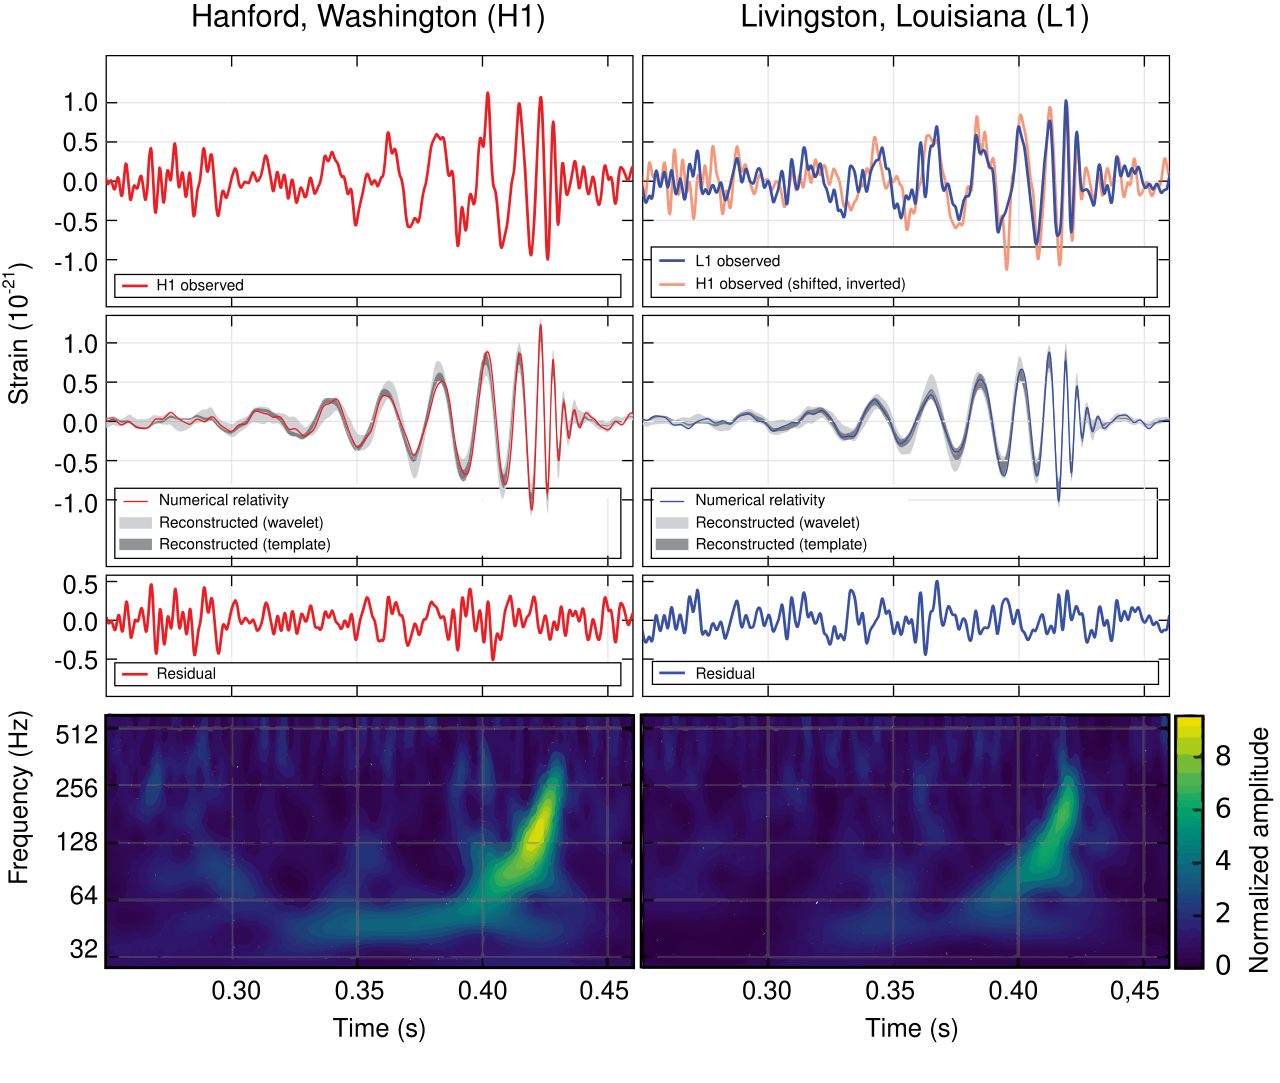
\includegraphics[width=0.8\textwidth]{Figures/LIGO_measurement_of_gravitational_waves.svg.png}
    \caption{Example of a gravitational wave signal detected by LIGO. The observed signal is compared with numerical relativity waveforms to identify the source as a binary black hole merger.}
    \label{fig:ligo_detector}
\end{figure}

Constructing theoretical models of binary black hole mergers is challenging because the relevant dynamics are strongly nonlinear and only partially accessible through analytic methods. In general relativity, exact analytic solutions are typically restricted to highly symmetric systems and cannot describe the full inspiral, merger, and ringdown of a generic binary black hole system. Numerical relativity therefore plays an essential role in modeling the late inspiral, merger, and ringdown, where fully nonlinear effects are important. A number of numerical relativity codes have been developed for this purpose, including the Einstein Toolkit, SpEC, GRChombo, BAM, GR Athena++, and Dendro GR \cite{Loffler2012,Boyle2019,Brugmann2008,Clough2015,Daszuta2021_GRAthena,Fernando2023}.

Simulating binary black hole mergers is computationally demanding. These simulations require solving a coupled system of nonlinear partial differential equations in three spatial and one time dimension, across multiple length scales, including the scale of the individual black holes, the orbital scale of the binary, and the radiation zone where gravitational waves are extracted \cite{BaumgarteShapiro2010,BaumgarteShapiro2021}. In this work, we make use of the Dendro numerical relativity framework, which combines adaptive mesh refinement with scalable parallel algorithms for binary black hole simulations \cite{Fernando2019,Fernando2019b,Fernando2023}.

For standard general relativity (GR), substantial progress has been made in modeling binary black hole mergers, and extensive
waveform catalogs now cover much of the binary black hole parameter space. In GR, the parameter space for binary black holes covers spin and mass ratio. Current catalogs have
good coverage for near equal mass systems. Here we define the mass ratio as
$q=M_{\mathrm{larger}}/M_{\mathrm{smaller}}\ge 1$. The LIGO  Virgo  KAGRA
(LVK) collaboration has reported hundreds of compact binary candidates using waveform
models informed by numerical relativity
\cite{Abbott2019,GWTC3,GWTC4,Boyle2019}.Future gravitational wave detectors, such as the Einstein Telescope and Cosmic Explorer, are expected to achieve significantly greater sensitivity than current ground based detectors \cite{Maggiore2020_ET,Reitze2019_CosmicExplorer,Evans2021_CEHorizon}. This increased sensitivity is expected to improve the signal to noise ratios of observed compact binary signals and to expand the range over which such systems can be detected. Meeting this challenge will require higher fidelity numerical simulations and more accurate waveform models \cite{Purrer2020_AccuracyRequirements,Black2025_ORBIT}.


In general, higher fidelity simulations, particularly those with larger mass ratios, require
finer grid resolution and therefore substantially greater computational cost. This trend is
illustrated in Fig.~\ref{fig:walltime}. Current simulations with mass ratios $q<8$ can
require weeks of runtime on modern supercomputers, and further increases in resolution
would significantly amplify this cost \cite{Boyle2019,Black2025_ORBIT}.

\begin{figure}[t]
    \centering
    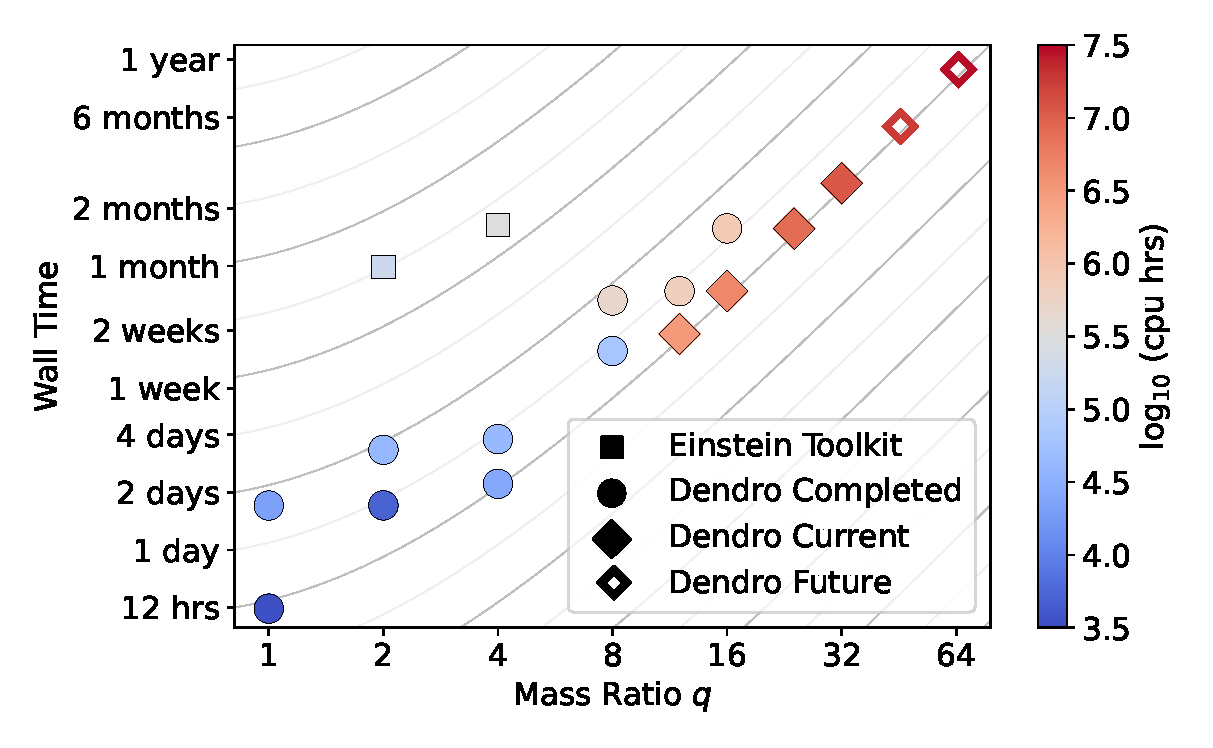
\includegraphics[width=0.8\textwidth]{Figures/walltime.pdf}
    \caption{Wall time of numerical relativity simulations as a function of mass ratio. As the mass ratio increases, the computational cost increases dramatically because the smaller black hole must be resolved with sufficient grid points. With current codes, performing a large number of high mass ratio simulations would therefore be prohibitively expensive.}
    \label{fig:walltime}
\end{figure}

To obtain more accurate waveforms, new techniques are needed: running existing codes at higher resolution will be insufficent. A drawback of the brute force approach simply increasing resolution is that the timesteps must also have a corresponding reduction. This, in turn, requires more timesteps, significantly increasing the total runtime and computational expense of the simulation.

One potential avenue for improving efficiency in numerical relativity codes lies in the computation of spatial derivatives. Most current implementations rely on explicit finite difference methods, while spectral methods although highly accurate are often difficult to implement. In this work, we explore compact finite difference (CFD) operators as an alternative. Compact schemes are implicit methods that can achieve higher spectral resolution than comparable explicit schemes \cite{Lele1992}. Across a variety of test problems, including the nonlinear sigma model, Maxwell's equations, and Einstein's equations, the compact finite difference schemes generally outperform the corresponding explicit methods.In some cases, the compact schemes achieve comparable accuracy to explicit schemes at approximately half the resolution. Despite their success in computational fluid dynamics and related fields, their use in numerical relativity remains limited \cite{Daszuta2023}.

In addition to the need for improved waveform modeling in GR, there is also a need for waveform models in alternative theories of gravity. Gravitational wave observations provide a powerful probe of gravity in the strongly nonlinear, dynamical regime, where deviations from general relativity (GR) may become apparent~\cite{Abbott2016,Abbott2025GWTC3GR,Yunes2025GWTests}. To search for such deviations, waveform templates from alternative theories of gravity are required~\cite{Yunes2009,Nair2019,Berti2015}. While studies have been carried out in theories such as Chern  Simons gravity~\cite{Alexander2009,Okounkova2019}, scalar  tensor theories~\cite{Barausse2013,Shibata2013,Berti2013,Palenzuela2014}, Einstein  Gauss  Bonnet gravity~\cite{Witek2019,Ripley2020b,East2021,Okounkova:2020rqw,Elley2022,Doneva2023sGB}, and Einstein  Maxwell  dilaton theory~\cite{Hirschmann2018,Julie2017}, waveform catalogs in these frameworks remain limited~\cite{Cardoso2012NRHEP,Corman2024NonlinearModificationsGR,Held2025}.


In this dissertation, we focus on Einstein  Maxwell  dilaton  axion (EMDA) theory. EMDA is of particular interest because it admits a well posed initial value formulation and arises as a low energy limit of string theory. In contrast to the no hair theorem in standard GR, which states that black holes can be completely defined by their mass spin and charge,  EMDA black holes possess additional degrees of freedom associated with the dilaton and axion fields.

We present a numerical relativity framework for simulating binary black hole mergers in EMDA theory. We analyze the resulting waveforms and investigate whether deviations from GR may be observable in gravitational wave signals.

\section{Background}
We focus on the study of black hole dynamics. As such, we begin with Einstein’s field equations:
\begin{equation}
    G_{ab} = 8 \pi T_{ab} + \Lambda g_{ab}.
\end{equation}
The left hand side describes the geometry of spacetime, while the right hand side encodes the matter and energy content.\cite{Wald1984,DInverno1992} We briefly examine each term in turn.

The tensor $G_{ab}$ is the Einstein tensor, which is constructed from quantities that encode the curvature of spacetime. The stress energy tensor $T_{ab}$ describes the distribution of matter and energy. The metric tensor $g_{ab}$ defines distances and the causal structure of spacetime. The constant $\Lambda$ is the cosmological constant, which is generally assumed to be very small. On the scales considered in this work, it is negligible, and we therefore set $\Lambda = 0$.

In standard general relativity simulations of binary black hole mergers, we consider vacuum spacetimes, for which
\begin{equation}
G_{ab} = 0.
\end{equation}
Although this equation appears innocuous, it represents a complex system of partial differential equations. In vacuum GR, these equations determine the spacetime geometry.

The Einstein tensor $G_{ab}$ is constructed from the Ricci tensor $R_{ab}$, the metric tensor $g_{ab}$, and the Ricci scalar $R$ according to
\begin{equation}
G_{ab} = R_{ab} - \frac{1}{2} g_{ab} R.
\end{equation}
The Ricci tensor and Ricci scalar are themselves contractions (contractions can be thought of as generalizations of dot products.) of the Riemann curvature tensor $R^{a}{} _{bcd}$. The Ricci tensor is obtained by contracting the first and third indices,
\begin{equation}
R _{ab} = R^{c}{} _{acb},
\end{equation}
and the Ricci scalar is obtained by a further contraction,
\begin{equation}
R = R ^{a}{}_{a}.
\end{equation}

The Riemann tensor is built from the Christoffel symbols and their derivatives. With our sign convention, it may be written as
\begin{equation}
R^{a}{}_{bcd}
=
\partial_c \Gamma^{a}{}_{bd}
- \partial_d \Gamma^{a}{}_{bc}
+ \Gamma^{a}{}_{ec}\Gamma^{e}{}_{bd}
- \Gamma^{a}{}_{ed}\Gamma^{e}{}_{bc},
\end{equation}
where $\Gamma^{a}{}_{bc}$ are the Christoffel symbols. These are determined by the metric and its first derivatives:
\begin{equation}
\Gamma^{a}{}_{bc}
=
\frac{1}{2} g^{ad}
\left(
\partial_b g_{dc}
+ \partial_c g_{bd}
- \partial_d g_{bc}
\right).
\end{equation}
Together, these relations show how the compact equation $G_{ab}=0$ encodes a system of nonlinear partial differential equations for the metric.

Although these geometric definitions expose the underlying structure of the Einstein equations, they still do not immediately resemble the second order system of partial differential equations used in numerical evolution. The equations can be reformulated into a strongly hyperbolic system suitable for time evolution, together with a set of equations that constrain the solution. We defer a complete discussion and expanation of how these evolution equations are formulated into a set of coupled partial differential equations to the Appendix~\ref{app:math_overview}. A key point though is that these constraint equations, such as the Hamiltonian and momentum constraints, must be satisfied by the initial data. In numerical simulations the constraints are not satisfied exactly because of finite resolution and truncation error. However, for a consistent numerical method, the constraint violations should decrease with increasing resolution and vanish in the continuum limit.

The preceding discussion is somewhat dense and we have skipped a few steps, so it is useful to consider a simpler example from Maxwell's equations. In vector notation, Maxwell's equations are
\begin{align}
\nabla \cdot \mathbf{E} &= 4\pi \rho, \\
\nabla \cdot \mathbf{B} &= 0, \\
\frac{\partial \mathbf{E}}{\partial t} &= \nabla \times \mathbf{B} - 4\pi \mathbf{J}, \\
\frac{\partial \mathbf{B}}{\partial t} &= - \nabla \times \mathbf{E}.
\end{align}

We present the full $3+1$ decomposition of Maxwell's equations in the Appendix~\ref{app:math_overview}. However, an important feature is already visible in this simpler form. There are eight scalar equations, but only six dynamical variables: $E_x$, $E_y$, $E_z$, $B_x$, $B_y$, and $B_z$. The remaining two equations constrain the allowed solutions.

Maxwell's equations can therefore be separated into evolution equations,
\begin{align}
\frac{\partial \mathbf{E}}{\partial t} &= \nabla \times \mathbf{B} - 4\pi \mathbf{J}, \\
\frac{\partial \mathbf{B}}{\partial t} &= -\nabla \times \mathbf{E},
\end{align}
and constraint equations,
\begin{align}
\nabla \cdot \mathbf{E} &= 4\pi \rho, \\
\nabla \cdot \mathbf{B} &= 0.
\end{align}

The constraint equations may also be written as
\begin{equation}
\mathcal{C}_E \equiv \nabla \cdot \mathbf{E} - 4\pi \rho = 0,
\end{equation}
\begin{equation}
\mathcal{C}_B \equiv \nabla \cdot \mathbf{B} = 0.
\end{equation}

These equations illustrate an important feature of many systems of partial differential equations. The electric and magnetic fields cannot be chosen arbitrarily. Instead, the initial data must satisfy the constraint equations before the evolution equations can be used to advance the solution in time. If the constraints are satisfied initially, they are preserved by the continuum evolution. In numerical simulations, finite resolution introduces small constraint violations, which should converge to zero as the resolution is increased.

General relativity has the same mathematical structure. Einstein's equations can be separated into evolution equations and constraint equations, and only initial data that satisfy the constraints represent physically valid solutions. Constructing such initial data is known as solving the Cauchy problem. More generally, the Cauchy problem is the initial value formulation of a system of partial differential equations, in which one specifies data on an initial spatial hypersurface that satisfy the constraint equations and then uses the evolution equations to determine the future development of the system.

Solving the Cauchy problem for Einstein's equations is nontrivial. In GR, the analogs of Gauss's law and the no monopole constraint are the Hamiltonian and momentum constraints. These constraints can be interpreted loosely as conditions related to energy and momentum conservation, and they must be satisfied by the initial data before the system can be evolved. Established techniques exist for constructing such data. In this work, we use the Bowen York equations to ensure that the initial data satisfy the momentum constraints. The Hamiltonian constraint then reduces to an elliptic equation that must be solved numerically. Further details on this procedure are given in the later chapters on initial data.

In EMDA theory, the Cauchy problem is further complicated by the presence of additional source terms. The stress energy tensor $T_{ab}$ encodes contributions from matter and nongravitational fields. In vacuum GR, this tensor vanishes, but in EMDA it includes contributions from the electromagnetic field, the dilaton, and the axion. Analytic single black hole solutions are known for special choices of the coupling parameters, such as $\alpha_0=\alpha_1=1$. However, numerical simulations allow us to vary these couplings and study how the resulting evolutions change. This dissertation addresses the challenges associated with constructing consistent initial data and evolving these systems numerically. For a more detailed discussion of the evolution equations and the mathematical machinery used to formulate them, see Appendix~\ref{app:math_overview}.

Once suitable initial data have been constructed and the system has been evolved, we extract the gravitational waveform. In this work, we compute the waveform using the Newman  Penrose formalism, in which outgoing gravitational radiation is represented by the Weyl scalar $\Psi_4$ \cite{Newman1962}. Details of how $\Psi_4$ is calculated are provided in Appendix~\ref{sec:appx:wave_extraction}.

The scalar $\Psi_4$ is related to the gravitational wave strain $h=h_+ i h_\times$ by
\begin{equation}
\Psi_4 = \frac{\partial^2 h}{\partial t^2},
\end{equation}
up to the sign conventions used for the null tetrad. From $\Psi_4$, we reconstruct the strain and compare simulated waveforms with one another and, in principle, with observed gravitational wave signals. To quantify the difference between two waveforms, we compute the mismatch:
we define the overlap and mismatch as:
\begin{equation}
    \mathcal{O}
    =
    \frac{
        \left|
        \langle h_1,h_2\rangle
        \right|
    }{
        \sqrt{
            \langle h_1,h_1\rangle
            \langle h_2,h_2\rangle
        }
    },
    \label{eq:app-waveex-time-overlap}
\end{equation}
The mismatch is then
\begin{equation}
    \mathcal{M}
    =
    1-\mathcal{O}.
    \label{eq:app-waveex-mismatch-basic}
\end{equation}
\begin{equation}
\mathrm{mismatch}(h_1,h_2) =    \max \mathcal{O}(h_1,h_2),
\end{equation}

where $\mathcal{O}$ is the normalized waveform overlap, and the maximum is taken over time shifts and polarization angles. The time shifts account for differences in the time of peak gravitational radiation, while the polarization angles account for rotations of the waveform polarization, equivalently phase rotations of the complex waveform.

The mismatch can be used to estimate the signal to noise ratio required to distinguish two waveforms. In the small mismatch limit, this distinguishability threshold is approximately
\begin{equation}
\rho \sim \frac{1}{\sqrt{2 \mathrm{mismatch}(h_1,h_2)}}.
\end{equation}
This estimate provides a useful way to interpret waveform differences, although it should not be regarded as an absolute detection criterion. In practice, interpreting differences between waveforms remains challenging because the parameter space is often degenerate. For example, it may not be immediately clear whether observed differences arise from spin, charge, or other physical effects.
Improving the accuracy of waveform comparisons requires improving the numerical simulations that produce the waveforms. We therefore also present our work incorporating compact finite difference operators into our numerical relativity code. To begin, we review the finite difference methods currently used in the code.

On a discrete grid, derivatives can be approximated using finite differences. For example, a second order accurate centered approximation to the first derivative is
\begin{equation}
\left.\frac{df}{dx}\right| _{i}
=
\frac{f _{i+1} - f_{i-1}}{2\Delta x}
+ \mathcal{O}(\Delta x^2).
\end{equation}

Higher order accurate formulas can be constructed by matching Taylor series expansions. For instance, a fourth order accurate centered stencil is
\begin{equation}
\left.\frac{df}{dx}\right| _{i}
=
\frac{-f _{i+2} + 8 f_{i+1} - 8 f_{i-1} + f_{i-2}}{12\Delta x}
+ \mathcal{O}(\Delta x^4).
\end{equation}
These finite difference approximations are standard tools for numerical solutions of partial differential equations \cite{BaumgarteShapiro2010}.

The above examples are explicit finite difference schemes, since the derivative at grid point $i$ is computed directly from nearby function values. Alternatively, one can approximate the first derivative using a compact, or implicit, finite difference scheme of the form
\begin{equation}
\beta f'_{i-2} + \alpha f'_{i-1} + f'_i
+ \alpha f'_{i+1} + \beta f'_{i+2}
=
c,\frac{f_{i+3} - f_{i-3}}{6\Delta x}
+ b,\frac{f_{i+2} - f_{i-2}}{4\Delta x}
+ a,\frac{f_{i+1} - f_{i-1}}{2\Delta x}.
\end{equation}
Here $f'_i$ denotes the numerical approximation to $df/dx$ at grid point $i$. Compact finite difference schemes of this type were developed to obtain higher spectral resolution than comparable explicit schemes \cite{Lele1992}.

The coefficients are determined by matching Taylor series expansions to the desired order of accuracy. For the above stencil, the consistency conditions include
\begin{align}
a + b + c &= 1 + 2\alpha + 2\beta,
&& \text{second order}, \\
a + 2^2 b + 3^2 c &= 2\frac{3!}{2!}\left(\alpha + 2^2\beta \right),
&& \text{fourth order}, \\
a + 2^4 b + 3^4 c &= 2\frac{5!}{4!}\left(\alpha + 2^4\beta \right),
&& \text{sixth order}.
\end{align}
This approach is more complex than an explicit finite difference stencil because the derivatives are obtained by solving an implicit system. The tradeoff is that compact schemes can provide improved accuracy and enhanced spectral resolution compared to explicit methods \cite{Lele1992}. This improvement in spectral resolution is illustrated in Fig.~\ref{fig:spectral_resolution}. There are many possible compact finite difference operators that can be constructed. In this work, we describe our methodology for identifying accurate and stable compact derivative operators and evaluate their performance relative to their explicit counterparts.

\begin{figure}[t]
\centering
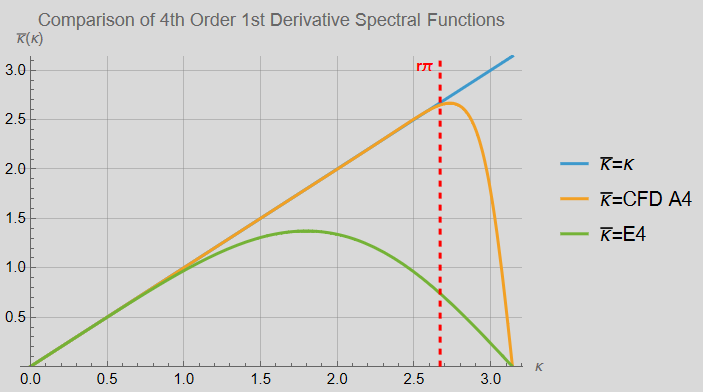
\includegraphics[width=0.8\textwidth]{Figures/1stDerivativeSpectralIntTest.png}
\caption{Spectral resolution of explicit and compact fourth order first derivative operators. The solid reference curve represents perfect resolution, and the dashed vertical line marks the cutoff frequency used in the optimization. The compact finite difference operator maintains better agreement with the ideal resolution curve over a wider range of wavenumbers.}
\label{fig:spectral_resolution}
\end{figure}

\section{Summary of Dissertation}

This dissertation primarily presents results from binary black hole simulations in Einstein  Maxwell  dilaton  axion (EMDA) theory, along with a study of compact finite difference methods for numerical relativity. The dissertation is organized as follows. Chapter~2 discusses the formulation of the initial data and presents results from head on collision simulations. Chapter~3 presents inspiral and merger results in EMDA theory. Chapter~4 explores interpolated EMDA models in which the coupling strengths are varied. Chapter~5 investigates the implementation of compact finite difference operators in numerical relativity codes.

Several of the results presented in this dissertation are currently in preparation for publication.

Each of these projects involved multiple collaborators. The EMDA work builds on earlier contributions by Hyun Lim at Los Alamos National Laboratory and was carried out collaboratively with Eric Hirschmann at Brigham Young University, David Van Komen at the University of Utah, Sebastian Vander Ploeg Fallon at Cornell University, and David Neilsen at Brigham Young University. The compact finite difference (CFD) project was conducted in collaboration with Eric Hirschmann, David Van Komen, David Neilsen, Nathaniel Garey, and Luke Papenfuss.

\section{Conventions}

In this work, we use geometrized units with $c=G=1$. Unless otherwise stated, lengths and masses are expressed in units of a characteristic mass scale $M$. In physical units, a length scale $d=M$ corresponds to $d=GM/c^2$, while a time scale $t=M$ corresponds to $t=GM/c^3$.

We use the metric signature $( ,+,+,+)$ and assume the Einstein summation convention unless otherwise stated. Spacetime indices $a,b,c,\ldots$ run over $0,1,2,3$, while spatial indices $i,j,k,\ldots$ run over $1,2,3$. The symmetric and antisymmetric parts of a tensor are defined as
\begin{equation}
T_{(ab)} \equiv \frac{1}{2}\left(T_{ab}+T_{ba}\right),
\qquad
T_{[ab]} \equiv \frac{1}{2}\left(T_{ab} T_{ba}\right).
\end{equation}

Partial derivatives are denoted by $\partial_i g$ or equivalently $g_{,i}$. Covariant derivatives are written as $\nabla_a f_b$ or equivalently $f_{b;a}$. The Lie derivative of a tensor $X^a$ along a vector field $\beta^a$ is denoted by $\mathcal{L}_{\beta}X^a$.

%In general, we use the following notation for geometric quantities. Objects associated with the spacetime manifold $\mathcal{M}$ are denoted by $g_{ab}$, ${}^{(4)}\Gamma^{a}{} _{bc}$, $\nabla_a$, ${}^{(4)}R _{ab}$, and related quantities. Objects associated with a spatial slice $\Sigma$ are denoted by $\gamma_{ij}$, $\Gamma^{i}{} _{jk}$, $D_i$, $R _{ij}$, and related quantities. Objects associated with a conformally related space are denoted by $\tilde{\gamma} _{ij}$, $\tilde{\Gamma}^{i}{} _{jk}$, $\tilde{D} _i$, $\tilde{R} _{ij}$, and related quantities.


\chapter{Head On Collisions and Stability Tests in EMDA Theory}
\section{Introduction}
\label{sec:intro}

While general relativity (GR) has passed all current experimental tests, there exist a large number of potentially viable extensions to it. Ongoing improvements in detector sensitivity, combined with numerical relativity will continue to enable increasingly precise tests of GR and proposed alternatives~\cite{Abbott2025GWTC3GR,Yunes2025GWTests,Abac2025GW250114,
Giri2025AdSBlackShells,Clough2024,Bambi2025Mimickers,
Yunes2013_LRR_GRTests,Yagi2016_BHTestsGR,Meidam2014,Berti2015,Yang2017}.
Indeed, advances in gravitational wave (GW) astronomy have led to a dramatic increase in the total number of detections of
signals from compact binary mergers, thereby providing access to strongly
gravitating, nonlinear domains. Since the first detection of gravitational waves, 
the Advanced LIGO and Virgo detectors have completed multiple
observing runs, producing a growing catalog of compact binary mergers
\cite{Abbott2019,GWTC2,GWTC3,GWTC4}. All observed mergers to date are consistent
with the predictions of GR within current uncertainties~\cite{Abbott2016,Abbott2016b,Abbott2019}. Nevertheless, compact binary coalescences continue to provide one of the most promising arenas for testing gravity beyond GR.

The increasing precision of gravitational wave observations has motivated effort to model compact object dynamics in theories beyond general relativity~\cite{Cardoso2012NRHEP,Corman2024NonlinearModificationsGR,Afshordi2024BlackHolesInsideOut,Bambi2025BlackHoleMimickers,Bernard2025GenericEFTGWTests}. Numerical relativity is
essential for this program because the late inspiral, merger, and ringdown
probe regimes in which the dynamics are intrinsically nonlinear and
analytic approximations are not uniformly reliable. Extending numerical
relativity to alternative theories of gravity, however, requires careful
control of the associated initial value problem. Reliable nonlinear
simulations require evolution systems with suitable hyperbolic structure,
controlled constraint propagation, and stable gauge dynamics. These
considerations have become central in beyond GR numerical relativity,
where the construction of robust evolution formulations is often a
prerequisite for extracting physical predictions.

The challenge is particularly relevant for theories motivated by effective field theory or higher curvature corrections to GR. Such theories introduce higher derivatives, additional characteristic modes, or principal parts whose hyperbolicity depends on the background solution and coupling strength. 
In some cases, higher derivatives may also be associated with Ostrogradsky type instabilities, unless the theory is interpreted within a controlled effective description or reformulated appropriately.
A significant number of previous studies have therefore been devoted to approaches that permit a more complete consideration of nonlinear aspects while maintaining control over the fundamental evolutionary problem. Examples of these include order reduction schemes in dynamical Chern Simons gravity~\cite{Alexander2009, Okounkova2019} and Einstein dilaton Gauss Bonnet theory~\cite{Okounkova:2020rqw,Okounkova2020}, modified gauge choices in Einstein scalar Gauss Bonnet~\cite{Ripley2020a,Ripley2020b}, the so called ``fixing the equations" approach~\cite{Cayuso2020}, and auxiliary field formulations for solving higher curvature systems including quadratic gravity~\cite{Held2021,Held2023,Held2025,East2023,Taillte2025} (see also~\cite{Corman2024} for a more in depth discussion and comparison of these and other approaches). These developments have expanded the range of beyond GR theories accessible to numerical relativity while emphasizing that dynamical consistency and observational phenomenology must be addressed together.

From this perspective, theories whose field equations can be written as second order evolution systems provide particularly useful laboratories for beyond GR numerical relativity. They allow one to study additional propagating degrees of freedom in fully nonlinear black hole (BH) spacetimes without relying entirely on perturbative or order reduced treatments of the gravitational field equations. 
Einstein--Maxwell--Dilaton--Axion (EMDA)~\cite{Sen1992,Sen1995}, arising as a low energy limit of heterotic string theory, is one such theory well suited to this purpose. Unlike many higher curvature modifications to GR, EMDA does not introduce higher derivatives into the metric field equations. Instead, it extends the Einstein Maxwell system by coupling the electromagnetic field to two additional propagating matter degrees of freedom: a dilaton and an axion. The resulting equations retain a structure closely related to the Einstein Maxwell system coupled to nonlinear matter fields. Consequently, EMDA can be formulated as a second order hyperbolic evolution problem using standard numerical relativity methods, together with appropriate evolution equations for the electromagnetic, dilaton, and axion fields.  In the limit of vanishing axion coupling, EMDA reduces to Einstein--Maxwell--Dilaton (EMD) theory.

Having a well posed initial value problem for EMDA is a crucial ingredient for sensible simulations, but it is also advantageous as it has analytically known black hole solutions at specific points in the theory space.  Certain of these are the stationary Kerr--Sen black holes.  They generalize the Kerr--Newman family of general relativity in that they carry 
nontrivial dilaton and axion fields in addition to mass, angular momentum,
and electromagnetic charge. As is well known, in standard GR coupled to Maxwell fields,
stationary black holes are characterized by their mass, angular momentum,
and electric charge \cite{Israel1967,Carter1971}. In contrast, extensions
of GR such as EMDA can admit black holes with additional matter fields.
Kerr--Sen solutions therefore
provide a natural setting in which to explore whether these additional degrees of
freedom behave as stable black hole hair in the nonlinear strong field
regime. Related questions have been studied in scalar Gauss--Bonnet gravity,
where scalarization and dynamical descalarization can occur during
compact binary evolutions
\cite{Elley2022,Silva2021DynamicalDescalarization}.
The nonlinear behavior of scalar and axionic hair in EMDA is connected to
several lines of previous work. Studies of EMD~\cite{Julie2017,Hirschmann2018}
provide an important foundation for extending nonlinear simulations to the
full EMDA system. Analytical investigations have examined aspects of the
perturbative stability of EMDA black holes in certain parameter regimes
\cite{PopeRohrerWhiting2025}. In addition, astrophysical studies have
explored possible observational signatures of Kerr--Sen BHs. For example,
analyses of Event Horizon Telescope (EHT) shadow data suggest that Sgr A*
may favor the Kerr--Sen solution, although similar data from M87* favor
Kerr while remaining consistent with Kerr--Sen within current observational
uncertainties~\cite{Sahoo2024PRD,Sahoo2025}.

Fully nonlinear simulations of binary BHs in EMDA remain limited. In particular, it is not yet well understood whether dilaton and axion hair persist through merger, disperse via radiation, or settle into a stable remnant configuration. Addressing these questions is important for assessing the nonlinear stability of Kerr--Sen BHs and for determining whether EMDA can provide distinct strong field signatures for future GW observations.  Although significant progress has been made in waveform modeling for selected beyond GR theories, including scalar Gauss Bonnet and Einstein dilaton Gauss Bonnet gravity, waveform coverage in alternative theories remains far less developed than in GR. Consequently, many current tests still rely on phenomenological parameterizations, post Newtonian approximations, or targeted numerical relativity simulations~\cite{Gasparotto2026MemoryHairyBBH,Agathos2014,Elley2022,Doneva2023sGB}.

In this study, we extend these investigations by simulating head on black hole mergers governed by the full EMDA equations. We analyze the resulting waveforms and examine the stability of the remnants, thereby gaining insight into the persistence of scalar hair within the theory. Specifically, we evolve several head on collisions of BHs in EMDA to determine the conditions under which the dilaton and axion fields survive merger.

The remainder of this chapter is organized as follows. In Sec.~\ref{sec:emda}, we review the EMDA action, equations of motion, and the formulation used for numerical evolution. In Sec.~\ref{sec:methods}, we describe our numerical methods, including the modified \texttt{Dendro GR} infrastructure, the construction of approximate binary BH initial data, and the extraction of gravitational, electromagnetic, dilaton, and axion radiation. In Sec.~\ref{sec:results}, we present simulations of head on Kerr--Sen BH collisions, analyze the emitted radiation, and examine the persistence of scalar hair in the remnant. We also study initially unscalarized configurations to determine whether scalar hair can be generated dynamically. We conclude in Sec.~\ref{sec:conclusion} with a summary of our results and directions for future work. Several important details such as the equations of motion, the analytic form of the Kerr--Sen solution, initial data and wave extraction techniques and issues associated with code performance are relegated to a number of appendices in order not to disrupt the continuity of the discussion.  %When discussing binary configurations, we use lowercase $m$ and $q$ to denote the mass and charge of an individual black hole, while uppercase $M$and $Q$ denote the mass and charge associated with the full spacetime of the binary system.

\section{Einstein--Maxwell--Dilaton--Axion}
\label{sec:emda}
The general theory we consider in this work is an extension of Einstein Maxwell on inclusion of two coupled scalar fields, the dilaton and the axion.  The action for the EMDA system is
\begin{equation}
\begin{aligned}
S=\int \mathrm{d}^4 x\,\sqrt{-g}\Big[
&{R\over8\pi}-2(\nabla\phi)^2-e^{-2\alpha_0\phi}F^2-\tfrac12 e^{4\alpha_1\phi}(\nabla\kappa)^2
-\kappa\,F_{ab}(*F)^{ab}
\Big],
\end{aligned}
\end{equation}
where the first term is the standard Hilbert action and \(\phi\) and \(\kappa\) are the dilaton and axion, respectively.
\(F_{ab}\) is the U(1) field strength, and \((*F)_{ab}\) is
its dual. The parameters $\alpha_0$ and $\alpha_1$ are real, positive constants
that set the coupling strengths and allow us to consider a family of EMDA
theories. Particular choices correspond to particular theories. For
instance, $\alpha_0=\alpha_1=0$ gives Einstein--Maxwell theory minimally
coupled to scalar and axion fields, while
$(\alpha_0,\alpha_1)=(\sqrt{3},0)$ corresponds to Kaluza--Klein.
In this work we take $(\alpha_0,\alpha_1)=(1,1)$, corresponding to a
low energy limit of heterotic string theory. For these coupling values, the
theory admits the Kerr--Sen family of rotating, charged black hole
solutions. These solutions reduce to Kerr when the electromagnetic charge
vanishes. In contrast to the Kerr--Newman solution of Einstein--Maxwell
theory, the Kerr--Sen geometry is accompanied by nontrivial dilaton and
axion fields whose structure is determined by the black hole charge and
spin. We now summarize the Kerr--Sen black-hole solution, which provides an exact rotating, charged black-hole solution of EMDA theory. This solution serves as a useful analytic reference for the charged rotating black holes we consider.

\subsection{Kerr--Sen Black Holes}
We present the Kerr--Sen solution in the Einstein frame, written in Boyer--Lindquist type coordinates. The metric takes the form

\begin{align}
ds^2 &= -\left(1-\frac{2mr\cosh^2\alpha}{\rho^2}\right)dt^2 + \rho^2\left(\frac{dr^2}{\Delta}+d\theta^2\right) \notag \\
&\quad+\frac{\Sigma}{\rho^2}\sin^2\theta\, d\varphi^2
-\frac{4amr\cosh^2\alpha}{\rho^2}\sin^2\theta\, dt\, d\varphi
\end{align}
where the metric functions are defined by
\begin{align}
\Delta &= r^2 - 2mr + a^2, \\
\rho^2 &= r^2 + a^2\cos^2\theta + 2mr\sinh^2\alpha, \\
\Sigma &= \left(r^2 + a^2 + 2mr\sinh^2\alpha\right)^2
         - \Delta a^2 \sin^2\theta.
\end{align}
The associated gauge, dilaton, and axion fields are given by
\begin{align}
A_a dx^a &= \frac{mr \sinh 2\alpha}{\sqrt{2}\,\rho^2}
\left(dt - a \sin^2\theta \, d\varphi \right), \\
\label{Kerr Sen_dilaton}
e^{-2\phi} &= \frac{\rho^2}{r^2 + a^2 \cos^2\theta}, \\ 
\kappa &= -2ma \sinh^2\alpha \, \frac{\cos\theta}{r^2 + a^2 \cos^2\theta}.
\end{align}

The parameters $m$, $\alpha$, and $a$ arise as integration constants. The physical mass $M$, electric charge $Q$, angular momentum $J$, and magnetic dipole moment $\mu$ are related to these parameters via
\begin{align}
M &= m \cosh^2\alpha, \\
Q &= \frac{m}{\sqrt{2}} \sinh 2\alpha, \\
J &= aM, \\
\mu &= aQ.
\end{align}

With respect to the Boyer--Lindquist radial coordinate, $r$, the event horizon is located at the familiar 
\begin{equation}
r_H = m + \sqrt{m^2 - a^2},
\end{equation}
and the condition for the existence of a nonextremal black hole %(i.e., the absence of a naked singularity) 
is
\begin{equation}
m^2 > a^2 \quad \Leftrightarrow \quad M^2 > |J| + \frac{Q^2}{2}.
\end{equation}
The inverse relations are
\begin{align}
m &= M - \frac{Q^2}{2M}, \\
\sinh 2\alpha &= \frac{2\sqrt{2}\,QM}{2M^2 - Q^2}, \\
a &= \frac{J}{M}.
\end{align}


\section{Numerical methods}
\label{sec:methods}

With the aim of studying the nonlinear dynamics of EMDA in black hole
collisions, we express EMDA as a Cauchy problem and evolve the
metric using the BSSN formulation~\cite{Shibata1995_BSSN,
Baumgarte1999_BSSN, Baumgarte2010}, supplemented by evolution equations for the electromagnetic, dilaton, and axion fields. We also employ puncture gauge conditions~\cite{Campanelli2006,Baker2006}.

For completeness, this section presents the full equations of motion and their $3+1$ decomposition.

\section{EMDA Equations of Motion}
\label{sec:eom}
The action for EMDA in the Einstein frame is given as:
\begin{equation}
S=\int \mathrm{d}^4 x\,\sqrt{-g}
\left[
\frac{R}{8\pi}
-2(\nabla\phi)^2
-e^{-2\alpha_0\phi}F^2
-\frac{1}{2}e^{4\alpha_1\phi}(\nabla\kappa)^2
-\kappa F_{ab}({}^*F)^{ab}
\right].
\end{equation}
where $\phi$ and $\kappa$ are the dilaton and axion, respectively.
The tensor $F_{ab}$ is the U(1) field strength, and $(*F)_{ab}$ is its
dual. In this work we set the coupling constants to
$\alpha_0=\alpha_1=1$, corresponding to a low energy limit of heterotic
string theory.

The Einstein equations are:
\begin{equation}
G_{ab}
=
8\pi G
\left[
2\left(\nabla_a\phi\nabla_b\phi-\frac{1}{2}g_{ab}(\nabla\phi)^2\right)
+
2e^{-2\alpha_0\phi}\left(F_{ac}F_b{}^c-\frac{1}{4}g_{ab}F^2\right)
+
\frac{1}{2}e^{4\alpha_1\phi}
\left(\nabla_a\kappa\nabla_b\kappa-\frac{1}{2}g_{ab}(\nabla\kappa)^2\right)
\right].
\label{eq:Einstein}
\end{equation}

while the matter equations can be written
\begin{align}
0
&=
\nabla^a\nabla_a\phi
+
\frac{1}{2}\alpha_0 e^{-2\alpha_0\phi}F^2
-
\frac{1}{2}\alpha_1 e^{4\alpha_1\phi}(\nabla\kappa)^2,
\label{eq:phi}
\\[1ex]
0
&=
\nabla^a\left(e^{4\alpha_1\phi}\nabla_a\kappa\right)
-
F_{ab}({}^*F)^{ab},
\label{eq:kappa}
\\[1ex]
0
&=
\nabla_a\left(e^{-2\alpha_0\phi}F^{ab}\right)
+
({}^*F)^{ab}\nabla_a\kappa.
\label{eq:Maxwell}
\end{align}

We include a form of hyperbolic constraint damping into the Maxwell equations so that violations propagate away at the speed of light. In particular, we introduce two scalar fields $\Phi$ and $\Psi$ into Eq.~\eqref{eq:Maxwell} and the identity $\nabla_a({}^*F)^{ab}=0$ as follows:
\begin{align}
\nabla_a\left(F^{ab}+g^{ab}\Psi\right)
&=
\eta_1 n^a\Psi
+
2\alpha_0\nabla_a\phi\,F^{ab}
-
e^{2\alpha_0\phi}({}^*F)^{ab}\nabla_a\kappa,
\\[1ex]
\nabla_a\left(({}^*F)^{ab}+g^{ab}\Phi\right)
&=
\eta_2 n^a\Phi.
\end{align}
where $\eta_1$ and $\eta_2$ are taken as positive constants and serve as tunable parameters to effect the damping of the electromagnetic constraints. Note that on the right hand sides, we have also included $n^a$, the usual unit timelike normal to the spatial hypersurfaces in anticipation of performing the usual $3+1$ split of spacetime. It is worth noting that these damped versions of Maxwell are now no longer strictly four covariant.
We introduce the usual $3+1$ decomposition of spacetime by defining the line element as 
\begin{align}
{\rm d}s^2 = -\alpha^2 {\rm d} t^2 + \gamma_{ij} ({\rm d}x^i + \beta^i {\rm d}t) ({\rm d}x^j + \beta^j {\rm d}t) 
\end{align}
with lapse, $\alpha$, shift, $\beta^i$, 3-metric, $\gamma_{ij}$, unit timelike normal $n_a = (-\alpha,0,0,0)$ and extrinsic curvature $K_{ab} = - \gamma_a{}^c \gamma_b{}^d\nabla_c n_d$.  

Using the BSSN formulation, we solve the standard 
BSSN evolution equations for the usual $\chi, {\tilde \gamma}_{ij}, K, {\tilde A}_{ij}$ and ${\tilde \Gamma}^i$ variables with EMDA matter terms.\footnote{Note that in this section only, $\chi$ represents the conformal factor and not the dimensionless spin parameter.}  These equations take the form 

\begin{align}
\partial_0\tilde{\gamma}_{ij} &= -2\alpha\,\tilde{A}_{ij},\\[4pt]
\partial_0 \chi &= \tfrac{2}{3}\alpha\,\chi\,K,\\[4pt]
\partial_0 K &= [\ldots] + 4\pi\alpha\,(\rho + T),\\[4pt]
\partial_0\tilde{A}_{ij} &= [\ldots] - 8\pi\chi\alpha\left( T_{ij} - \tfrac{1}{3}\,\gamma_{ij} T_k{}^k\right),\\[4pt]
\partial_0 \tilde{\Gamma}^i &= [\ldots] - 16\pi\alpha\,\chi^{-1} S^{\,i},
%\tilde{\Gamma}^i &= \tilde{\gamma}^{jk}\tilde{\Gamma}^{\,i}{}_{jk}
\end{align}
where $\partial_0 \equiv \partial_t - {\cal L}_{\beta}$ with ${\cal L}_{\beta}$ the Lie derivative along the shift and the $[\ldots]$ are a stand in for the relevant right hand sides which can be found in standard references, e.g.~\cite{Baumgarte2010} 

The quantities $S^i$, $T_{ij}$, and $\rho$ are defined as
\begin{equation}
\begin{aligned}
S^i
&\equiv -\gamma^{ia} T_{ab} n^b  \\
&=   2\Pi D^i\phi
   + 2e^{-2\alpha_0\phi}\epsilon^{ijk}E_jB_k  %\\
%&\qquad\qquad
   + \tfrac{1}{2}e^{4\alpha_1\phi}\Xi D^i\kappa ,
\label{eq:Si}
\end{aligned}
\end{equation}
\begin{equation}
\begin{aligned}
T_{ij}
&\equiv T_{ab} \gamma^a{}_i \gamma^b{}_j  \\
&= 2\Bigl[
      D_i\phi D_j\phi
      - \tfrac{1}{2}\tilde{\gamma}_{ij}\bigl((D\phi)^2-\Pi^2\bigr)
   \Bigr] 
- 2e^{-2\alpha_0\phi}\Bigl( 
       E_iE_j + B_iB_j 
      - \tfrac{1}{2}\tilde{\gamma}_{ij}
        \bigl(E_kE^k + B_kB^k\bigr)
   \Bigr)  \\
&\quad\,
+ \tfrac{1}{2}e^{4\alpha_1\phi}\Bigl[
      D_i\kappa D_j\kappa
      - \tfrac{1}{2}\tilde{\gamma}_{ij}\bigl((D\kappa)^2-\Xi^2\bigr)
   \Bigr] .
\label{eq:Tij}
\end{aligned}
\end{equation}

\begin{equation}
    \rho \equiv \Pi^2 + (D\phi)^2 
    + e^{-2 \alpha_0 \phi}\big( E_a  E^a +  B_a  B^a\big) + \tfrac{1}{4} e^{4 \alpha_1 \phi}\big(\Xi^2 + (D\kappa)^2\big).
\end{equation}

We use standard puncture gauge conditions for the lapse and the shift:
\begin{align}
\partial_t\alpha &=\beta^i \partial_i - 2\alpha K , \\[4pt]
\partial_t \beta^i &= \beta^j \partial_j \beta^i + \tfrac{3}{4} B^i , \\[4pt] 
\partial_t B^i &= \beta^j \partial_j B^i + \partial_t {\tilde\Gamma}^i - \beta^j \partial_j {\tilde \Gamma}^i - \eta B^i .
\end{align}
We also employ a slow start lapse condition~\cite{Etienne2024} to reduce transients at early times.  This amounts to adding the term 
\begin{equation}
- \chi^{1/2} \bigl(\varpi \, e^{-t^2/2\sigma^2}\bigr)\,(\alpha - \chi^{1/2})
\end{equation}
to the equation for the lapse.  Following~\cite{Etienne2024}, we take the constants $\varpi=3/5$ and $\sigma=20$.

For the matter equations we start with the dilaton and axion:
\begin{align}
    \partial_0 \phi &= - \alpha \Pi , \\
    \partial_0 \kappa &= - \Xi 
\end{align}
\begin{equation}
\begin{aligned}
\partial_0 \Pi
=& \, \alpha K \Pi
- \alpha \chi\, \tilde{\gamma}^{ij} \partial_i \partial_j \phi
- \chi\, \tilde{\gamma}^{ij} \partial_i \alpha\, \partial_j \phi 
+ \alpha \chi\, \tilde{\Gamma}^i \partial_i \phi
+ \frac{\alpha}{2}\tilde{\gamma}^{ij}
  \partial_i \chi\, \partial_j \phi \\
&+ \frac{\alpha\alpha_0}{\chi}
  e^{-2\alpha_0\phi}
  \tilde{\gamma}_{ij}
  \left(E^iE^j - B^iB^j\right) + \frac{\alpha\alpha_1}{2}
  e^{4\alpha_1\phi}
  \left(
    \chi\,\tilde{\gamma}^{ij}
    \partial_i\kappa\,\partial_j\kappa
    - \Xi^2
  \right).
\end{aligned}
\end{equation}


\begin{equation}
\begin{aligned}
\partial_0 \Xi
&= \alpha K \Xi
- \alpha \chi\, \tilde{\gamma}^{ij} \partial_i \partial_j \kappa
- \chi\, \tilde{\gamma}^{ij}\, \partial_i \alpha\, \partial_j \kappa
+ \alpha \chi\, \tilde{\Gamma}^i \partial_i \kappa
+ \frac{\alpha}{2}\, \tilde{\gamma}^{ij}\, \partial_i \kappa\, \partial_j \chi
\\[6pt]
&\quad
- 4 \alpha \alpha_1 \chi\, \tilde{\gamma}^{ij}\,
  \partial_i \kappa\, \partial_j \phi
+ 4 \alpha \alpha_1 \Pi \Xi
+ \frac{4\alpha}{\chi}\,
  e^{-4\alpha_1 \phi}\,
  \tilde{\gamma}_{ij} B^i E^j .
\end{aligned}
\end{equation}
The equations for the electromagnetic fields, including hyperbolic divergence cleaning become
\begin{equation}
\begin{aligned}
\partial_0 \Psi
&= - \alpha\, \partial_i E^i
+ \frac{3\alpha}{2\chi}\, E^i \partial_i \chi
+ 2 \alpha_0 \alpha\, E^i \partial_i \phi
+ \alpha e^{2\alpha_0 \phi}\, B^i \partial_i \kappa
- \alpha \eta_1 \Psi .
\end{aligned}
\end{equation}
\begin{equation}
\begin{aligned}
\partial_0 \Phi
&= \alpha\, \partial_i B^i
- \frac{3\alpha}{2\chi}\, B^i \partial_i \chi
- \alpha \eta_2 \Phi .
\end{aligned}
\end{equation}
\begin{equation}
\begin{aligned}
\partial_0 E^i
&= \alpha K E^i
+ 2 \alpha \alpha_0 \chi^{1/2}\,
  \epsilon^{jik}\tilde{\gamma}_{kl} B^l \partial_j \phi
- 2 \alpha \alpha_0 E^i \Pi
\\[6pt]
&\quad
+ \alpha e^{2\alpha_0 \phi} \chi^{1/2}\,
  \epsilon^{ijk}\tilde{\gamma}_{kl} E^l \partial_j \kappa
- \alpha e^{2\alpha_0 \phi} \Xi B^i
- \alpha \chi\, \tilde{\gamma}^{ij} \partial_j \Psi
- \chi^{1/2}\, \epsilon^{jik}\tilde{\gamma}_{kl} B^l \partial_j \alpha
\\[4pt]
&\quad
- \alpha \chi^{1/2}\, \epsilon^{jik} B^l \partial_j \tilde{\gamma}_{kl}
- \alpha \chi^{1/2}\, \epsilon^{jik}\tilde{\gamma}_{kl} \partial_j B^l
+ \alpha \chi^{-1/2}\, \epsilon^{jik}\tilde{\gamma}_{kl} B^l \partial_j \chi .
\end{aligned}
\end{equation}

\begin{equation}
\begin{aligned}
\partial_0 B^i
&= \alpha K B^i
+ \alpha \chi\, \tilde{\gamma}^{ij} \partial_j \Phi
\\[6pt]
&\quad
- \chi^{1/2}\, \epsilon^{ijk}\tilde{\gamma}_{kl} E^l \partial_j \alpha
+ \alpha \chi^{-1/2}\, \epsilon^{ijk}\tilde{\gamma}_{kl} E^l \partial_j \chi
- \alpha \chi^{1/2}\, \epsilon^{ijk} E^l \partial_j \tilde{\gamma}_{kl}
- \alpha \chi^{1/2}\, \epsilon^{ijk}\tilde{\gamma}_{kl} \partial_j E^l .
\end{aligned}
\end{equation}
Initial data are prepared for head on black hole collisions and are described below. 


\subsection{Code Description}
\label{sec:code_description}

We perform our black hole merger simulations using \texttt{Dendro GR}, a well developed numerical relativity framework. \texttt{Dendro GR} combines an octree based adaptive
mesh infrastructure with automatic code generation for the evolution
equations~\cite{Fernando2019,Fernando2019b,Fernando2023}. The computational domain is refined dynamically using wavelet adaptive multiresolution (WAMR) in which the evolved fields are represented on an adaptive hierarchy of octree blocks. Wavelet coefficients computed from the evolved variables provide a local estimate of the truncation error 
or unresolved field content~\cite{DeBuhr2018RelativisticHydroWavelets,Anderson2006RelativisticMHDAMR, Fernando2023}.
Regions where these wavelet coefficients exceed a prescribed tolerance are refined, while regions in which wavelet coefficients remain below a coarsening threshold are de refined. This tends to concentrate resolution near the black holes, in the wave extraction region, and in regions where the electromagnetic, dilaton, or axion fields develop large spatial gradients, while smoother regions are evolved on coarser grids.

Spatial derivatives are computed using sixth order finite difference
stencils, and time integration is performed using a fourth order
Runge--Kutta scheme. We include Kreiss--Oliger dissipation to damp
poorly resolved high frequency modes and improve numerical stability
\cite{KreissOliger1973}. Additional details of the \texttt{Dendro GR}
infrastructure, including its WAMR implementation, scalability, and previous applications to binary black hole evolutions, can be 
found in~\cite{Fernando2019,Fernando2019b,Fernando2023,Black2025_ORBIT}.

During the evolutions, we monitor the Hamiltonian and momentum constraints together with the electromagnetic divergence constraints throughout the computational domain. These quantities provide a global check on the consistency of the evolution and are used to assess the efficacy of the WAMR refinement parameters. Representative plots of the constraints and their violation are shown below:

\subsection{Constraint quantities}

We monitor the constraint violations throughout the evolution.
In particular, we compute the $L_2$ norms of the Hamiltonian and momentum
constraints, together with the electromagnetic constraints.
When evaluating these norms, we excise small neighborhoods around the punctures
to avoid unduly weighting them by these regions. Representative
constraint violations for the full simulation are shown in
Figs.~\ref{fig:constraint_ham_mom} and \ref{fig:constraint_divb}.

% ---------------------------------------------------------
% Constraint violations over the full simulation
% ---------------------------------------------------------

\begin{figure}[tbp]
  \centering
  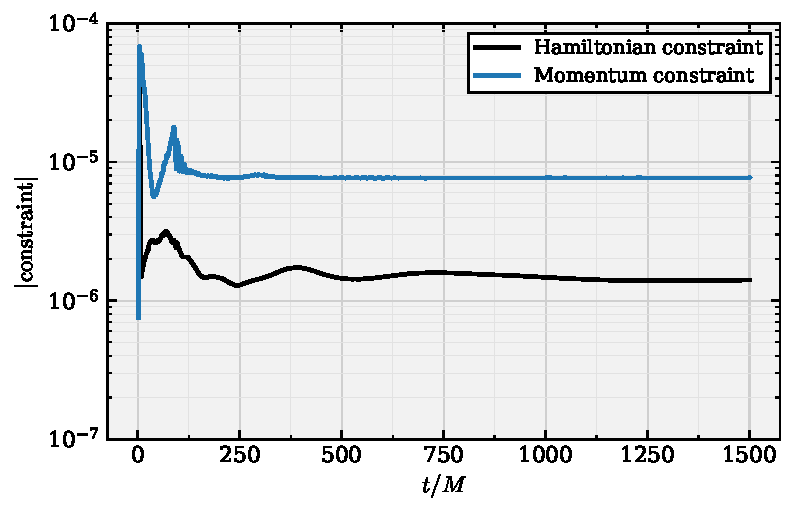
\includegraphics[width=0.92\columnwidth]{Figures/Chapter_1/emda_prof_Constraints_Hamiltonian_plus_MomentumSum.pdf}
  \caption{
  The Hamiltonian constraint $\mathcal{H}$ and summed momentum constraint
  violation measured over the full simulation. The $L_2$ norm is taken with respect to the number of points  The constraints remain
  controlled throughout the evolution, including the merger phase.
  }
  \label{fig:constraint_ham_mom}
\end{figure}

\begin{figure}[tbp]
  \centering
  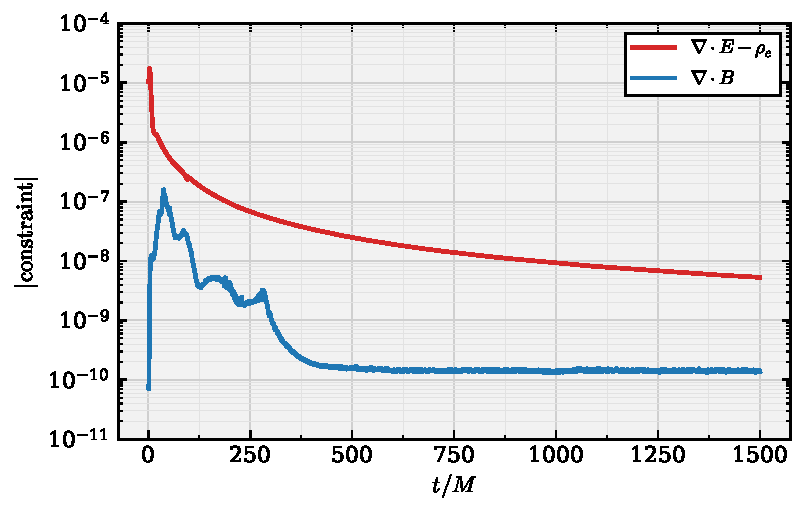
\includegraphics[width=0.92\columnwidth]{Figures/Chapter_1/emda_prof_Constraints_DivE_DivB.pdf}
  \caption{
  The volume weighted $L_2$ norms of the electromagnetic constraints, namely the no-monopole constraint that involves the divergence of the magnetic field, $\nabla\cdot B$, and the Gauss constraint that invokes the divergence of the electric field.  Both are measured over the full simulation. 
  }
  \label{fig:constraint_divb}
\end{figure}

We also compute quasilocal quantities on apparent horizons using the
\texttt{BHaHAHA} apparent horizon finder~\cite{Etienne2026BHaHAHA}, which
we have extended to evaluate the horizon mass, spin, and electric charge.
These quantities provide independent diagnostics of remnant relaxation and
of the conservation of the black hole charges during the evolution.

As a check on our overall numerical strategy, we perform a limited type of convergence study by varying both the wavelet
tolerance and maximum refinement level for a short head on binary evolution.  We confirm that with increased numbers of refinement levels and tighter refinement criteria constraint violations are reduced.  
The details of this study are presented below:

\subsection{Code performance}
A full convergence study for binary black hole evolutions is computationally expensive and is therefore not attempted here. Instead, we assess the behavior of the code by varying two parameters that directly affect the adaptive mesh refinement: the wavelet tolerance, $\varepsilon$, and the maximum refinement level, $\ell_{\rm max}$. The wavelet tolerance is the threshold value in our WAMR scheme on the  coefficients of the wavelet expansion that determines whether refinement or coarsening occurs.  The maximum refinement level sets the largest number of refinement levels that can be obtained in a simulation.  We confirm that for both, making these refinement criteria more stringent leads to a corresponding reduction in the constraint violations.

The tests done here use the first \(20M\) of a head-on evolution of two equal-mass, charged black holes. The black holes have an initial coordinate separation of $16M$, individual masses of \(m_1=m_2=0.50\), and charge-to-mass ratios \(q_1/m_1=q_2/m_2=0.1\). Both black holes have dimensionless spin \(\chi=0.4\) and are initially at rest. In computing the constraint diagnostics, we again exclude a small neighborhood of each puncture from calculation of the norms.
Throughout this section, the constraint measure shown is the sum of the volume weighted Hamiltonian constraint and the three volume weighted momentum constraints. This provides a single diagnostic for the overall constraint violation during the evolution.

Comparisons of simulations with respect to different wavelet tolerances are shown in Figure~\ref{fig:constraint_wavelet_tolerance}.  Decreasing $\varepsilon$ allows the grid to refine more aggressively in regions with larger truncation error.  For the three different wavelet tolerances of $\varepsilon \in \{3\times10^{-5}, 1\times10^{-5}, 3\times10^{-6}\}$ we can see that the constraints are indeed reduced as $\varepsilon$ decreases.  

\begin{figure}[tbp]
  \centering
  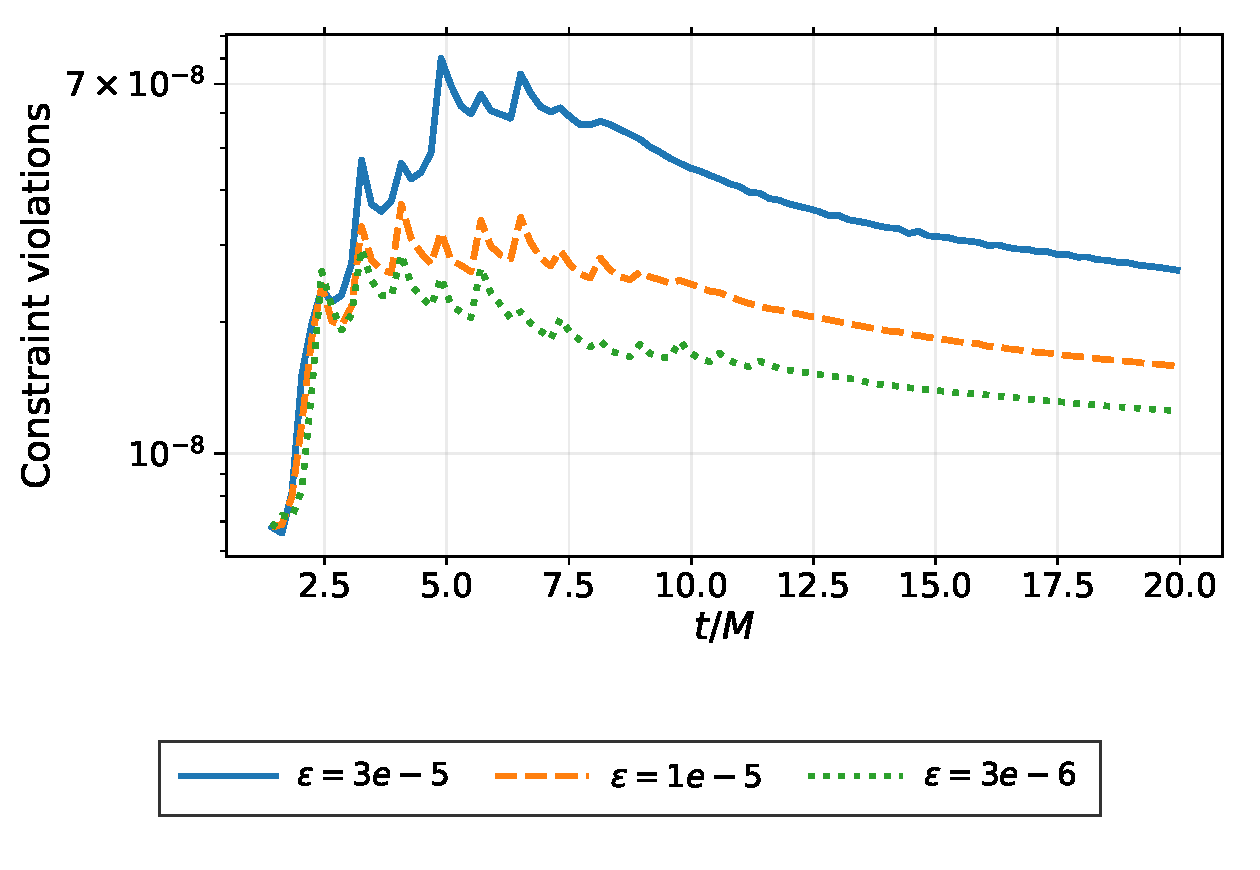
\includegraphics[width=0.92\columnwidth]{Figures/Chapter_1/Wavelet_tolerance.pdf}
  \caption{
  The sum of the volume weighted Hamiltonian and momentum constraint violations
  over the first \(20M\) of a head-on evolution of two equal-mass charged
  black holes with charge-to-mass ratio \(q/m=0.1\) and dimensionless spin
  \(\chi=0.4\). The simulations use wavelet tolerances of $\varepsilon \in \{3\times10^{-5}, 1\times10^{-5}, 3\times10^{-6} \}$. These simulations were done with a maximum refinement level of $\ell_{\rm max} = 15$.
  Lowering the wavelet tolerance improves the resolution of dynamically
  important regions and reduces the overall constraint violation.
  }
  \label{fig:constraint_wavelet_tolerance}
\end{figure}

Comparing simulations according to different maximum refinement levels is another means of changing the resolution in an AMR setting.  Figure~\ref{fig:constraint_maxdepth} compares simulations with maximum refinement levels of $\ell_{\rm max} \in \{14, 15, 16, 17\}$ corresponding to finest grid spacings of $h \in \{ 0.0325, 0.0162, 0.00813, 0.00407 \}$, respectively. Increasing the allowed maximum depth provides additional resolution near the black holes and in regions where the fields develop sharp spatial structures. The resulting decrease in the constraints provides further evidence that the simulations improve with increased resolution.

\begin{figure}[tbp]
  \centering
  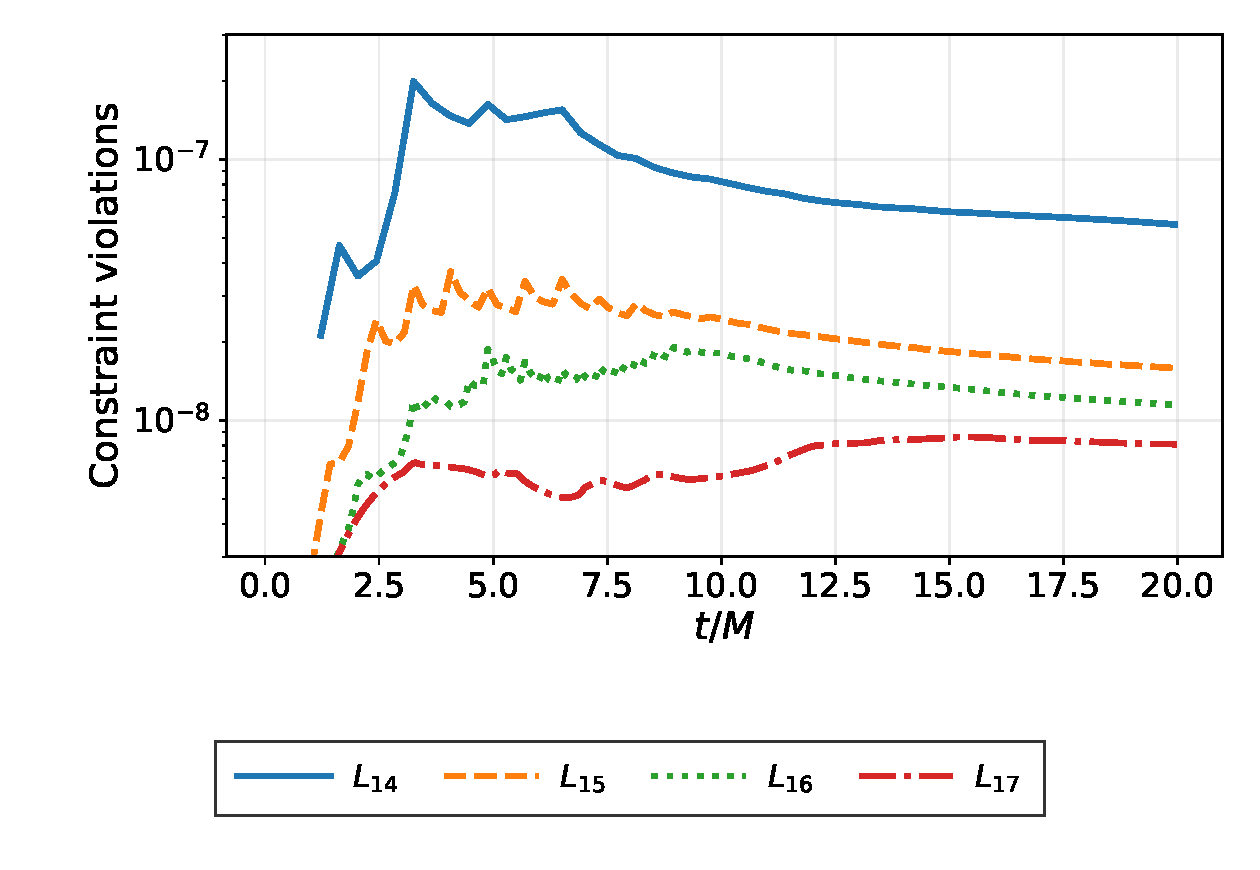
\includegraphics[width=0.92\columnwidth]{Figures/Chapter_1/total_hamiltonian_momentum_volume_weighted.pdf}
  \caption{
  The sum of the volume weighted Hamiltonian and momentum constraint violations over the first \(20M\) of a head-on evolution of two equal-mass charged black holes with charge-to-mass ratio \(q/m=0.1\) and dimensionless spin  \(\chi=0.4\) each. The simulations compare maximum refinement levels $\ell_{\rm max} \in \{14, 15, 16, 17\}$ corresponding to finest grid spacings of $h \in \{ 0.0325,0.0162,0.00813,0.00407 \}$, respectively. The wavelet tolerance is set here to $\varepsilon = 1\times 10^{-5}$.  Increasing the maximum refinement level reduces the overall constraint violation by allowing additional grid refinement in under-resolved regions.
  }
  \label{fig:constraint_maxdepth}
\end{figure}

\subsection{Initial Data}

Valid initial data must satisfy the relevant constraint equations. In particular, the Hamiltonian, momentum, and Maxwell constraints are 
\begin{align}
R + K^2 - K_{ij}K^{ij} &= 16 \pi \rho, \\
D_j\left(K^{ij} - \gamma^{ij}K\right) &= 8 \pi S^i, \\
%\end{align}
%\begin{equation}
D_i E^i &= \rho_E, \\
\qquad
D_i B^i &= 0,
\end{align}
where \(R\) is the Ricci scalar associated with the spatial metric
\(\gamma_{ij}\), \(K_{ij}\) is the extrinsic curvature, \(K\) is its trace,
and \(D_i\) is the covariant derivative compatible with \(\gamma_{ij}\).
The electric and magnetic fields are \(E^i\) and \(B^i\) with electric charge density, $\rho_E$, while quantities \(\rho\) and \(S^i\) are the matter energy and current densities,
respectively.  The latter, in EMDA, take the form
\begin{align}
%\begin{split}
\rho_E \equiv& \, 2\alpha_0 E^i D_i \phi + e^{2\alpha_0\phi} B^i D_i \kappa \\
%
\rho \equiv& \, \Pi^2 + (D\phi)^2
+ e^{-2 \alpha_0 \phi}\big( E_i E^i + B_i B^i\big),  \nonumber + \tfrac{1}{4} e^{4 \alpha_1 \phi}\big(\Xi^2 + (D\kappa)^2\big), \\
%
S^i \equiv& 2 \Pi D^i \phi
+ 2 e^{-2 \alpha_0 \phi} \epsilon^{ijk} E_j B_k
+ \tfrac{1}{2} e^{4 \alpha_1 \phi} \Xi D^i \kappa.
\end{align}
where \(\Pi\) and \(\Xi\) denote the momenta conjugate to the
dilaton \(\phi\) and axion \(\kappa\), respectively.

Binary black hole initial data in EMDA have not been extensively studied,
although several methods have been developed for constructing initial data
for charged black holes in related settings
\cite{Alcubierre2009,Mukherjee2022_ConformallyCurvedChargedSpinning,
Zilhao2014,Zilhao2012,Bozzola2019}. In this work, we adapt some of these techniques to the EMDA system by using an elliptic solver based on a modified version of the two charged punctures solver introduced 
in~\cite{Bozzola2019}.
Our implementation includes contributions from the dilaton and axion fields. A more detailed discussion of the initial data construction is provided below:
\section{Initial Data}
\label{sec:appx:id}

It is necessary to have good initial data for our EMDA BH binaries.  Of course, exact solutions are not known.  But we can generalize standard approaches for the construction of initial data in vacuum GR to these additional fields on making certain approximations.  We follow closely the approach based on the conformal transverse traceless decomposition  used with punctures.  Indeed, we extend this approach as it has been incorporated into the {\tt TwoChargedPunctures} code of Bozzola and Paschalidis~\cite{Bozzola2019,ferreira2026electromagneticdualitydegeneracydynamical}.  We mostly follow their notation below.

As usual, we decompose the metric, but using notation slightly modified from the previous appendix.  In particular we define 
%systemsAs a first step, we assume conformally flat space; that is, we decompose the metric as
\begin{equation}
    \gamma_{ij}= \psi^4 \bar{\gamma}_{ij},
\end{equation}
with $\psi$ the conformal factor and the conformal metric assumed to be the flat metric, ${\bar\gamma}_{ij} = \eta_{ij}$.  The latter assumption simplifies the following computations and is a reasonable choice for the systems we study. It is a limiting assumption preventing the construction of highly spinning black holes~\cite{ValienteKroon2004,Price2000}. 
Notwithstanding, Bowen--York black holes can reach spin values of order $\chi \sim 0.9$ \cite{Dain2002}. As our simulations remain below this limit, the approximation should be reasonable.  
While we anticipate the appearance of ``junk radiation'' partly in consequence of this assumption~\cite{Bozzola2021}, we find that it does decay  
as the fields relax to quasi equilibrium which results in decreased constraint violation over the course of the evolutions. We adopt the maximal slicing condition, $K=0$, and define a conformally rescaled tracefree extrinsic curvature, ${\bar A}_{ij}=\psi^{2}(K_{ij} - \tfrac{1}{3} \gamma_{ij} K)$.  Ignoring the latter's radiative degrees of freedom, we can express it in terms of a vector, $V^i$, as
\begin{equation}
    \bar{A}_{ij} = \partial_i V_j + \partial_j V_i - \frac{2}{3}\eta_{ij}\partial_k V^k.
\end{equation} 

The initial data problem then reduces to determining $V^i$ and $\psi$ for the gravitational pieces.  In particular, the Hamiltonian and momentum constraint equations take the form
\begin{equation}     
\partial_k\partial^k \psi + \tfrac{1}{8} \psi^{-7} \bar{A}_{ij} \bar{A}^{ij} = - 2\pi \psi^5 \rho 
\end{equation}
\label{hamiltonian_constraint} 
\begin{equation}
    \partial_k \partial^k V^i + \tfrac{1}{3}\eta^{ij}\partial_j(\partial_k V^k ) = 8 \pi S^i . 
\label{momemtum_constraint}
\end{equation}

The momentum constraint is linear and independent of $\psi$.  This permits dividing the solution between homogeneous (vacuum gravitational) and inhomogeneous (matter) contributions:
\begin{equation}
    V^i = V^i_{\text{GR}} + V^i_{\text{M}}.
\end{equation}
For $V^i_{\text{GR}}$, we use the standard Bowen--York solutions~\cite{Bowen1980} while for the matter contribution, we must solve Eq.~\ref{momemtum_constraint} with 
\begin{equation}
    S^i = 2 \, \Pi \, D^i \phi 
    + 2 e^{-2 \alpha_0 \phi} \epsilon^{ijk} E_j B_k 
    + \tfrac{1}{2}e^{4 \alpha_1 \phi} \, \Xi \, D^i \kappa.
\end{equation}
If we assume a moment of time symmetry and neglect contributions from the magnetic field this source term vanishes.  On imposing asymptotically flat boundary conditions, the solution to the matter part therefore becomes $V^i_{\text{M}}=0$.  

We must also impose the electromagnetic constraints. At this point we  depart somewhat from~\cite{Bozzola2019} because the EMDA version of these constraints are no longer linear, containing rather a nontrivial current that couples the dilaton and axion to the electromagnetic fields: 
\begin{align}
\nabla_i E^i &= 2\alpha_0 E^i \partial_i \phi + e^{2\alpha_0 \phi} B^i \partial_i \kappa \\
\nabla_i B^i &= 0 
\end{align} 
Were the source in the Gauss constraint zero, we would 
follow \cite{Alcubierre2009,Zilhao2012} and perform a conformal rescaling of the fields as
\begin{equation}
    \bar{E}^i = \psi^6 E^i, 
    \quad
    \bar{B}^i = \psi^6 B^i.  
\end{equation}
This results in the sourceless Maxwell constraints taking the form 
\begin{equation}
    \partial_i \bar{E}^i = 0, 
    \quad
    \partial_i \bar{B}^i = 0,
\end{equation}
independent of $\psi$ and therefore solvable separately from the spacetime variables. Since these equations are linear, solutions may be superposed. The advantages of this are significant so we choose to make the approximation that this source term is, in fact, negligible and we solve the EMDA electromagnetic constraints in the way just described.  Of course, this failure to self consistently solve these constraints necessarily introduces violations.  Partly for this reason, we have introduced hyperbolic divergence cleaning to drive these violations smaller over the course of the evolution.  We have measured these violations on the initial slice. For the simulations considered in this work we confirm that they are consistently small and driven smaller via the constraint damping. The expected damping behavior is demonstrated in Figure~\ref{fig:constraint_divb}. There is an initial violation of the EM constraints, which damps over time.    

The Hamiltonian constraint above, not being linear, must be treated differently.  We assume that we have two black holes charged under the U(1) gauge field as well as possessing scalar dilaton and axion fields.  Following \cite{Bozzola2019}, we approximate this with a conformal factor of the form 
\begin{equation}
    \psi^2 = (1 + u + \bar{\eta} )^2 - \bar{\xi}^2 
\end{equation}
for which we define 
\begin{align}
   \bar{\eta} &= \frac{m_1}{2R_1} + \frac{m_2}{2R_2}, \\
   \bar{\xi}  &= \frac{q_1}{2R_1} + \frac{q_2}{2R_2}, \\ 
   \bar{\kappa} &= 1+ u + {\bar\eta},
\end{align}
and where $m_i$, $q_i$ and $R_i$ here are the masses, electric charges and the coordinate distances from the origin of the BHs.  This is intended to correspond to two electrically charged BHs with the singular part of the conformal factor separated out with $u$ giving finite corrections, including the necessary corrections for the additional scalar fields. 

Rearranging the Hamiltonian constraint in terms of $u$, we find
\begin{equation}
    \partial_k \partial^k u
    =
    -\frac{1}{\bar{\kappa}}
    \left(
        \partial_a \bar{\kappa} \partial^a \bar{\kappa}
        - \partial_a \bar{\xi} \partial^a \bar{\xi}
        - \partial_a \psi \partial^a \psi
        + \frac{1}{8} \psi^{-6} \bar{A}_{ij} \bar{A}^{ij}
        + 2\pi \psi^{6} \rho
    \right).
\end{equation}
with
\begin{equation}
    \rho \equiv \bigl[ \Pi^2 + (D\phi)^2 \bigr]
    + e^{-2 \alpha_0 \phi}\big[ E_a E^a +  B_a  B^a\big]
    + \tfrac{1}{4} e^{4 \alpha_1 \phi}\big[\Xi^2 + (D\kappa)^2\big].
\end{equation}
Using simplifying assumptions similar to above, namely a moment of time symmetry and neglecting the magnetic field, $\rho$ reduces to
\begin{equation}
    \rho = (D\phi)^2 + e^{-2 \alpha_0 \phi} \, E_a E^a + \tfrac{1}{4} e^{4\alpha_1 \phi} \, (D\kappa)^2 .
\end{equation}
Again, this follows \cite{Bozzola2019} quite closely, except that we have now included dilaton and axion contributions in $\rho$. Specifically, we employ a Reissner--Nordström electric field for the electric component and add a dilaton field for a single, spinless black hole. In practice, the axion is initialized to zero and allowed to relax to a quasi equilibrium state during an evolution.  

The electric field is initially set to be:
\begin{equation}
     E^i = \psi^{-6} \Bigl[ \frac{q_1}{R_1^2} + \frac{q_2}{R_2^2} \Bigr].
\end{equation}
while the dilaton fields are initially set as:
\begin{align}
\phi &= \phi_1(r_1,\theta_1) + \phi_2(r_2, \theta_2) 
\end{align}
where Eq.~\ref{Kerr Sen_dilaton} gives the form for a dilaton field for a single Kerr--Sen black hole (albeit in Boyer--Lindquist type coordinates) for our current theory parameters of $(\alpha_0,\alpha_1) = (1,1)$. 

\section{Radiated Quantities}
To analyze the radiation emitted, we compute the Newman--Penrose scalar
\(\Psi_4\), along with the electromagnetic radiation. We extract their multipolar components at \(r \approx 100M\).  Additional details of the waveform extraction procedure are  given in the following section.  A summary of the initial data parameters used in our simulations is provided in Appendix~\ref{sec:appx:sim_tab}.

At an extraction radius $R_{\mathrm{ex}}$, each radiative quantity is decomposed into spin weighted spherical harmonics with the appropriate spin weight:
\begin{align}
    \Psi_4(t,\theta,\varphi)
    &=
    \sum_{\ell,m}
    \Psi_4^{\ell m}(t)\,
    {}_{-2}Y_{\ell m}(\theta,\varphi),
    \label{eq:app waveex psi4-decomp}
    \\
    \Phi_1(t,\theta,\varphi)
    &=
    \sum_{\ell,m}
    \Phi_1^{\ell m}(t)\,
    {}_{0}Y_{\ell m}(\theta,\varphi),
    \label{eq:app waveex phi1-decomp}
    \\
    \Phi_2(t,\theta,\varphi)
    &=
    \sum_{\ell,m}
    \Phi_2^{\ell m}(t)\,
    {}_{-1}Y_{\ell m}(\theta,\varphi),
    \label{eq:app waveex phi2-decomp}
    \\
    \mathcal{D}(t,\theta,\varphi)
    &=
    \sum_{\ell,m}
    \mathcal{D}^{\ell m}(t)\,
    {}_{0}Y_{\ell m}(\theta,\varphi),
    \label{eq:app waveex dilaton decomp}
    \\
    \mathcal{A}(t,\theta,\varphi)
    &=
    \sum_{\ell,m}
    \mathcal{A}^{\ell m}(t)\,
    {}_{0}Y_{\ell m}(\theta,\varphi).
    \label{eq:app waveex axion decomp}
\end{align}
The strain is decomposed similarly as
\begin{equation}
    h(t,\theta,\varphi)
    =
    \sum_{\ell,m}
    h_{\ell m}(t)\,
    {}_{-2}Y_{\ell m}(\theta,\varphi).
    \label{eq:app waveex strain decomp}
\end{equation}
For each gravitational wave mode, Eq.~\eqref{eq:app waveex psi4-strain} implies
\begin{equation}
    \Psi_4^{\ell m}(t)
    =
    \ddot{h}_{\ell m}(t),
\end{equation}
or equivalently
\begin{equation}
    h_{\ell m}(t)
    =
    \int^t dt'
    \int^{t'} dt''\,
    \Psi_4^{\ell m}(t'') .
\end{equation}
Waveform comparisons in this work primarily use the dominant $(\ell,m)=(2,2)$ mode.

\subsection{Radiated Energy Fluxes}

The radiated energy fluxes in the gravitational, electromagnetic, dilaton, and axion channels are computed from the multipolar amplitudes. Following Ref.~\cite{Zilhao2012}, we use
\begin{align}
    F_{\mathrm{GW}}
    &=
    \frac{dE_{\mathrm{GW}}}{dt}
    =
    \lim_{r\to\infty}
    \frac{r^2}{16\pi}
    \sum_{\ell,m}
    \left|
        \int_{-\infty}^{t}
        \Psi_4^{\ell m}(t')\,dt'
    \right|^2,
    \label{eq:app waveex gw flux}
    \\
    F_{\mathrm{EM}}
    &=
    \frac{dE_{\mathrm{EM}}}{dt}
    =
    \lim_{r\to\infty}
    \frac{r^2}{4\pi}
    \sum_{\ell,m}
    \left|
        \Phi_2^{\ell m}(t)
    \right|^2,
    \label{eq:app waveex em flux}
    \\
    F_{\mathrm{D}}
    &=
    \frac{dE_{\mathrm{D}}}{dt}
    =
    \lim_{r\to\infty}
    \frac{r^2}{4\pi}
    \sum_{\ell,m}
    \left|
        \mathcal{D}^{\ell m}(t)
    \right|^2,
    \label{eq:app waveex dilaton flux}
    \\
    F_{\mathrm{A}}
    &=
    \frac{dE_{\mathrm{A}}}{dt}
    =
    \lim_{r\to\infty}
    \frac{r^2}{4\pi}
    \sum_{\ell,m}
    \left|
        \mathcal{A}^{\ell m}(t)
    \right|^2 .
    \label{eq:app waveex axion flux}
\end{align}
In numerical simulations, these quantities are evaluated at finite extraction radii. The expressions above should therefore be interpreted as asymptotic large radius definitions, with the finite radius values serving as numerical approximations.



\section{Results}
\label{sec:results}

We now describe the simulations of two broad classes of binary black holes in EMDA.  The first consist of two Kerr--Sen black holes with at least one having nontrivial dilaton and axion fields attached.  This is a nice, even stringent test of the persistence of these scalar fields through merger and the settling down of the final object to a new and different Kerr--Sen black hole.  The second is the simulation of two Kerr--Newman black holes with perturbative dilaton and axion fields in the vicinity.  This latter case is to test whether the merging black holes can acquire these scalar fields and whether the merger then results in a final Kerr--Sen remnant.  



% ---------------------------------------------------------
% Waveforms (2x2 subfigure grid)
% ---------------------------------------------------------
\begin{figure}[!htbp]
  \centering

  \subfloat[Real part of the $(2,0)$ mode of $\Psi_4$ extracted at $R_{\mathrm{ex}} = 100M$.%
    \label{fig:gw_l2m0}%
  ]{%
    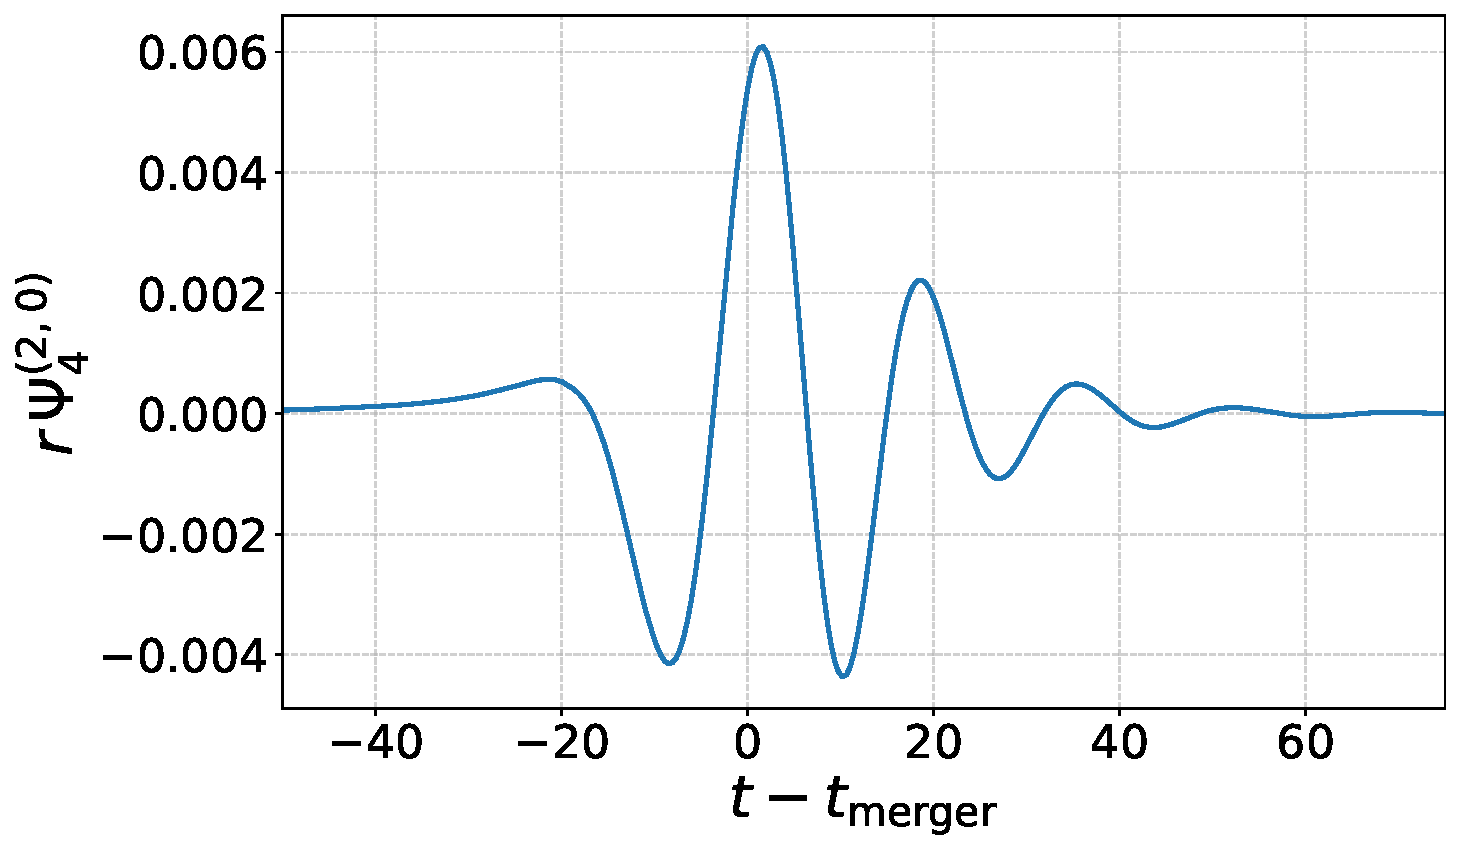
\includegraphics[width=0.48\linewidth]{Figures/Chapter_1/emda_prof_GW_l2_m0_r5.pdf}%
  }%
  \hfill
  \subfloat[Real part of the $(2,0)$ mode of $\Phi_1$ extracted at $R_{\mathrm{ex}} = 100M$.%
    \label{fig:phi1_l2m0}%
  ]{%
    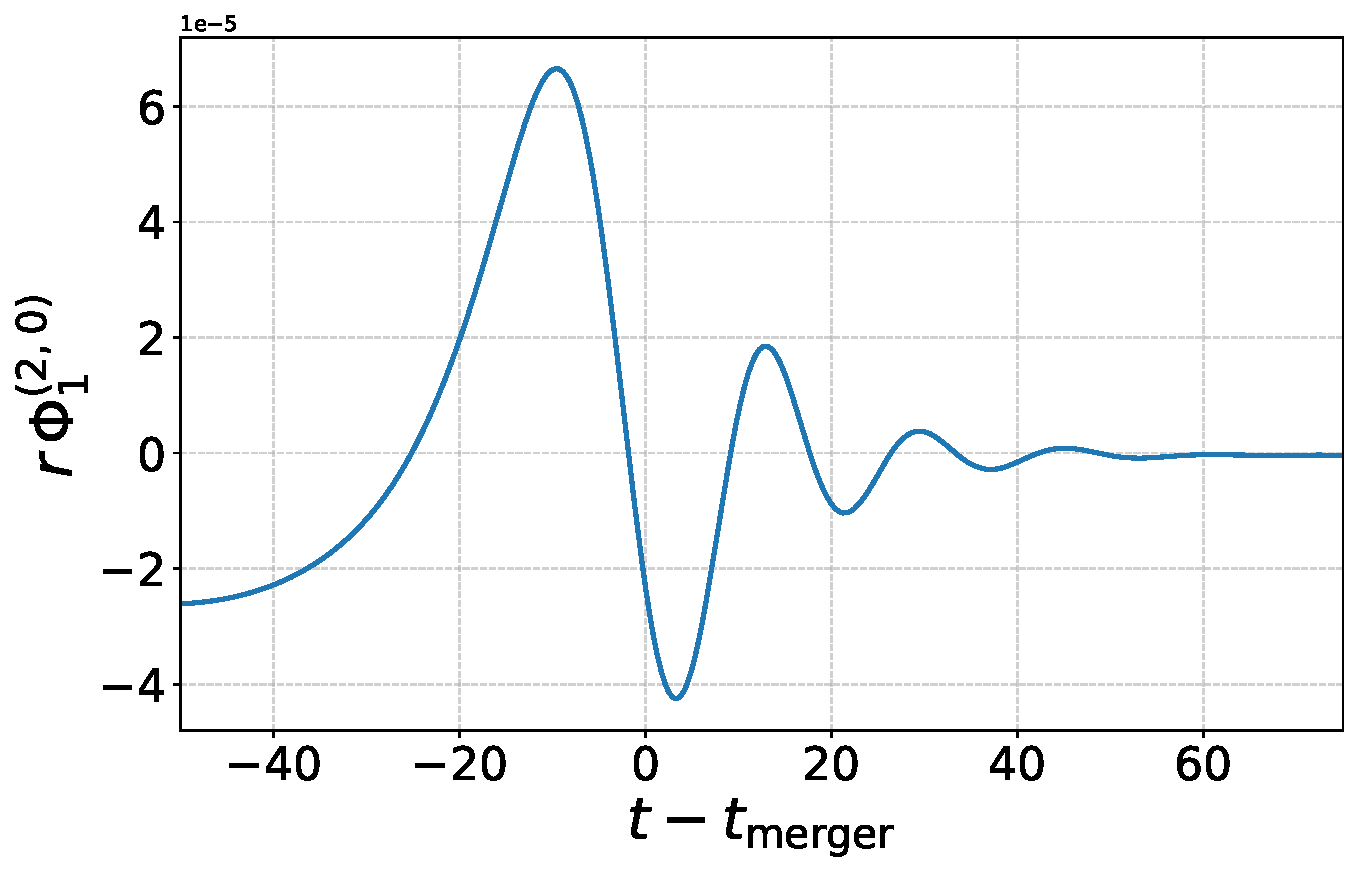
\includegraphics[width=0.48\linewidth]{Figures/Chapter_1/emda_prof_PHI1_l2_m0_r5.pdf}%
  }%

  \vspace{0.6em}

  \subfloat[Real part of the $(2,0)$ mode of $\Phi_2$ extracted at $R_{\mathrm{ex}} = 100M$.%
    \label{fig:phi2_l2m0}%
  ]{%
    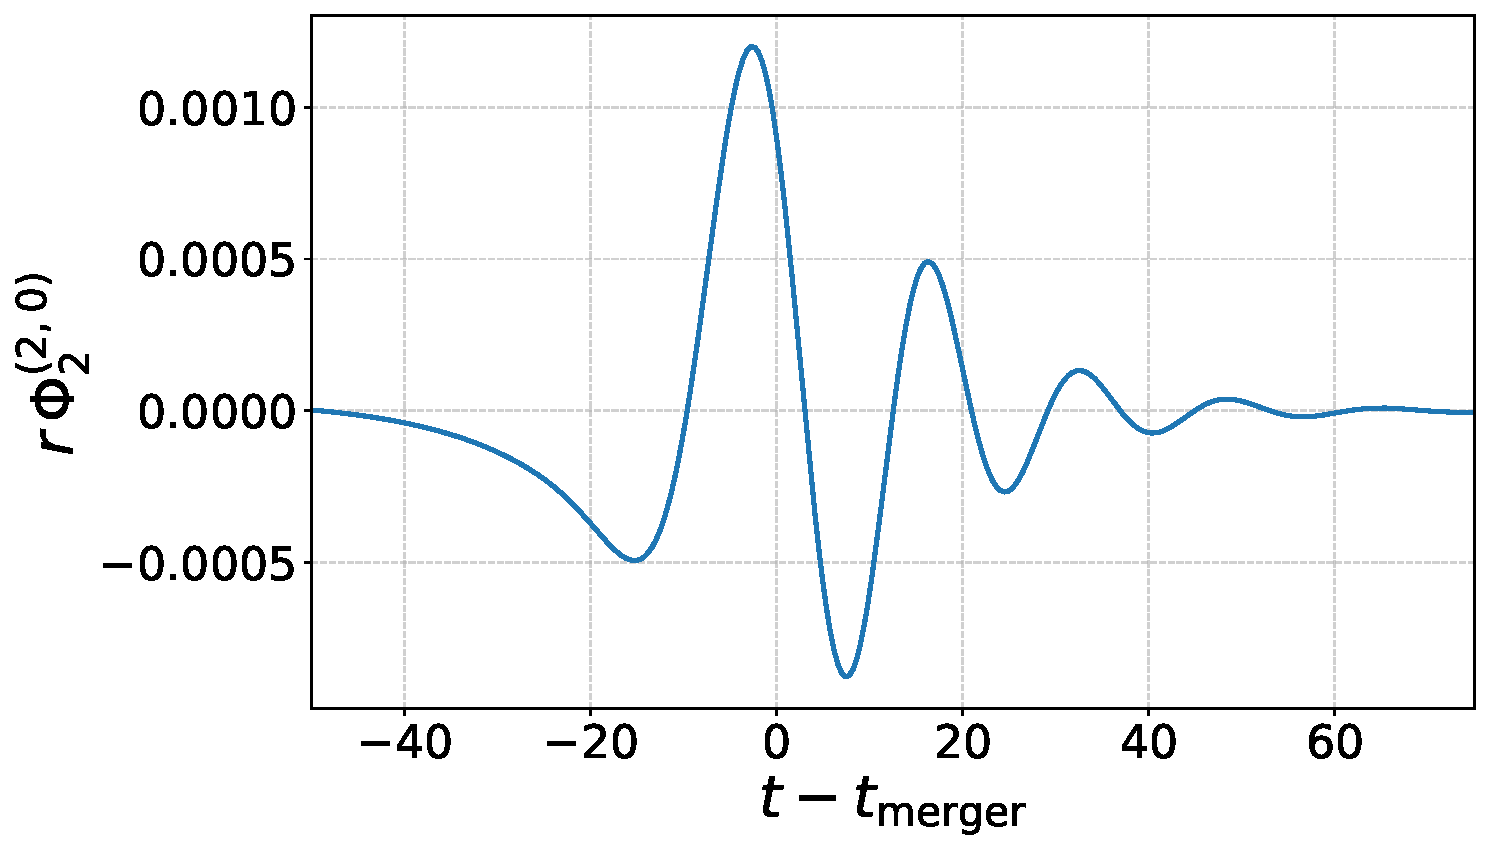
\includegraphics[width=0.48\linewidth]{Figures/Chapter_1/emda_prof_PHI2_l2_m0_r5.pdf}%
  }%
  \hfill
  \subfloat[Real part of the $(2,0)$ mode of $\phi$ extracted at $R_{\mathrm{ex}} = 100M$.%
    \label{fig:dil_l2m0}%
  ]{%
    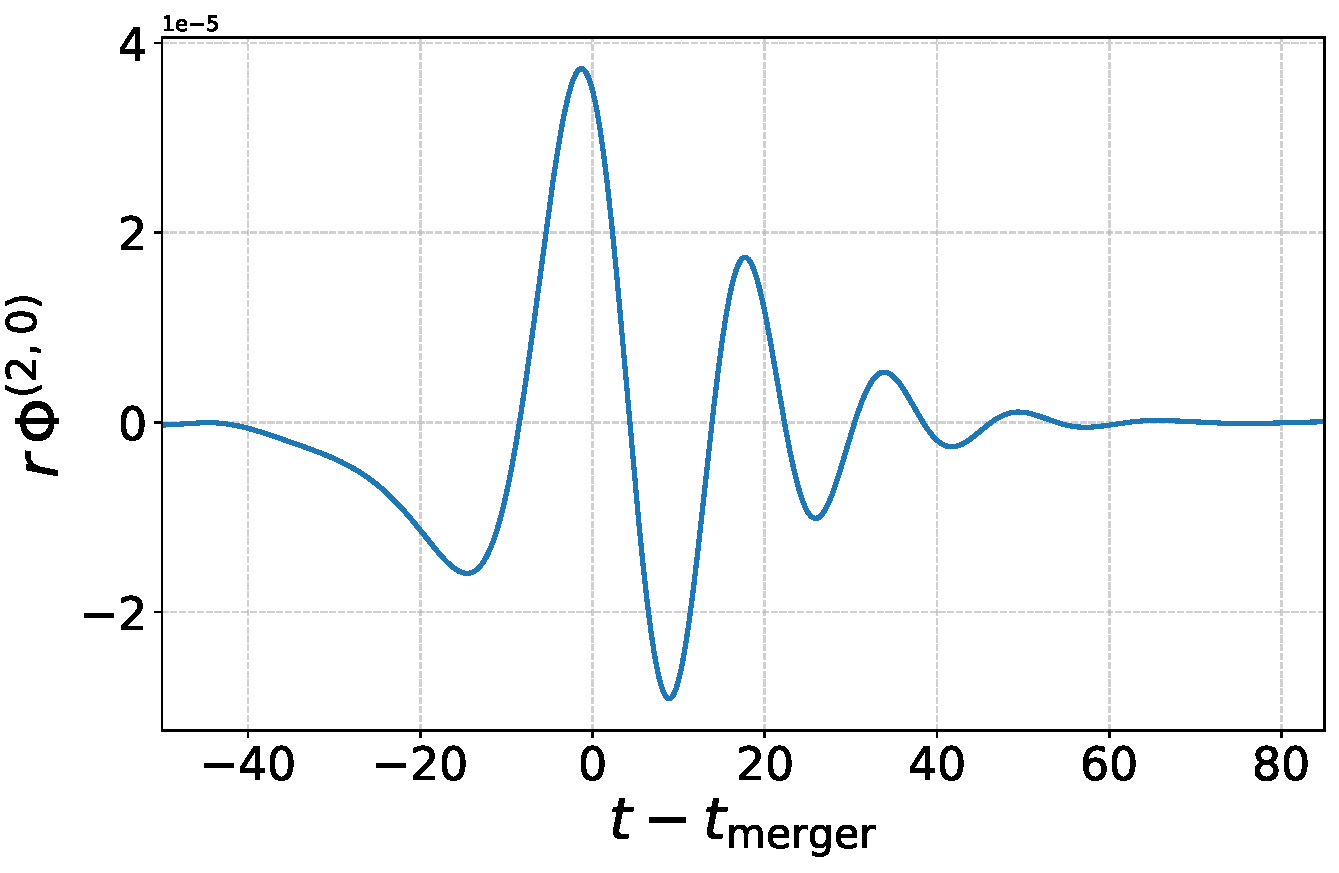
\includegraphics[width=0.48\linewidth]{Figures/Chapter_1/emda_prof_Dilaton_l2_m0_r5.pdf}%
  }%

  \caption{The real portions of the $(2,0)$ modes of the gravitational radiation $\Psi_4$, electromagnetic radiation $\Phi_1$ and $\Phi_2$, and dilaton field $\phi$, extracted at $R_{\mathrm{ex}} = 100M$ for a binary with charge to mass ratio $q_i/m_i = 0.1$, dimensionless spin $\chi = 0.4$, and an initial coordinate separation of $16M$.}
  \label{fig:waveforms_l2m0}
\end{figure}

\subsection{Initially Scalarized Black Holes}
We perform simulations across a range of binary Kerr--Sen black hole configurations in the initial data space.  For the current work, we focus on equal mass binaries with low to moderate charge and low spin.  In particular, the total mass of the system is normalized to $M=1$.  The charge to mass ratio on each black hole ranges between $0.0625 \leq q_i/m_i \leq 0.5$ where $m_i$ and $q_i$ are the initial masses and charges of the individual black holes.  For spinning cases, the spins of both black holes are usually taken to be equal and aligned.  The spin magnitude of each is taken to lie in the range $0.05 \leq \chi \leq 0.4$. A more complete summary of the parameter values used in our tests is provided in subsection below:
\subsection{Summary of Tests Done}
\label{sec:appx:sim_tab}
In addition to some of the tests mentioned earlier in the chapter, we have also performed a broader set of simulations to test how the late time dilaton and axion fields depend on the initial charges and spins of the binary components. In particular, we considered Kerr--Sen binaries with same sign and opposite sign charges, spin aligned and spin anti aligned configurations, as well as mergers involving neutral GR black holes. For binaries with opposite charges, the net charge vanishes and the remnant settles to a Kerr black hole, with neither a persistent dilaton nor axion field. For binaries with same sign charges but oppositely aligned spins, the axion field decays, while the dilaton field remains nontrivial, corresponding to an EMD like remnant. We further find that when charged, spinless black holes are merged with Kerr black holes, both axion and dilaton fields persist. Finally, we find that mergers of initially nonscalarized Kerr--Newman black holes produce remnants with both dilaton and axion hair. The configurations considered are summarized in Table~\ref{tab:bh_hair_combined}, where a green check mark indicates that the corresponding field remains persistent and nontrivial at late times.

\begin{center}
{\label{tab:bh_hair_combined}%
Binary black hole configurations }
\begingroup
\footnotesize
\setlength{\tabcolsep}{8pt}
\renewcommand{\arraystretch}{1.1}


% ---------- FIRST SECTION ----------
\textbf{(a) Kerr--Sen Same Sign Charge and Spin Aligned Black Hole Tests} \\[0.4em]
\begin{tabular}{lllcc}
$(\chi_1, q_1)$ & $(\chi_2, q_2)$ & \textrm{Dilaton $\boldsymbol{\phi}$} & \textrm{Axion $\boldsymbol{\kappa}$} \\ \hline
$\chi_1 = 0.10$, $q_1 \in \{0.0624, 0.125, 0.25, 0.50\}$ &
$\chi_2 = 0.10$, $q_2 \in \{0.0624, 0.125, 0.25, 0.50\}$ &
\cmark & \cmark \\[0.3em]
$\chi_1 = 0.20$, $q_1 \in \{0.0624, 0.125, 0.25, 0.50\}$ &
$\chi_2 \in \{0.10, 0.20\}$, $q_2$ as above &
\cmark & \cmark \\[0.3em]
$\chi_1 = 0.40$, $q_1 \in \{0.0624, 0.125, 0.25, 0.50\}$ &
$\chi_2 \in \{0.10, 0.20, 0.40\}$, $q_2 \in \{0.0624, 0.125, 0.25, 0.50\}$ &
\cmark & \cmark \\
\end{tabular}

\vspace{1.2em} % spacing between subtables

% ---------- SECOND SECTION ----------
\textbf{(b) Collisions with Other Black Holes} \\[0.4em]
\begin{tabular}{llcc}
\textrm{Black Hole 1 $(q,\chi)$} & \textrm{Black Hole 2 $(q,\chi)$} & $\boldsymbol{\phi}$ & $\boldsymbol{\kappa}$ \\
\hline
Kerr--Sen $(0.5,\,0.4)$   & Kerr--Sen $(0.5,\,0.4)$   & \cmark & \cmark \\
Kerr--Sen $(0.5,\,0.4)$   & Kerr $(0.0,\,0.4)$        & \cmark & \cmark \\
Kerr--Sen $(0.5,\,0.4)$   & Kerr--Sen $(-0.5,\,0.4)$  & \xmark & \xmark \\
Kerr--Sen $(0.5,\,-0.4)$  & Kerr--Sen $(0.5,\,0.4)$   & \cmark & \xmark \\
EMD $(0.5,\,0.0)$          & Kerr $(0.0,\,0.4)$        & \cmark & \cmark \\
KN $(0.5,\,0.4)^{\dagger}$& KN $(0.5,\,0.4)^{\dagger}$& \cmark & \cmark \\
\end{tabular}

\endgroup

\vspace{0.5em}
\footnotesize
\noindent
$^{\dagger}$ These configurations were initialized as nonscalarized
Kerr--Newman black holes.

Abbreviations: EMD denotes Einstein--Maxwell--dilaton, corresponding here to
a charged black hole with dilaton hair; KN denotes Kerr--Newman, corresponding
to a black hole with charge and spin; and Kerr--Sen denotes a rotating charged
black hole with dilaton and axion hair.
\end{center}


Figure~\ref{fig:waveforms_l2m0} shows the waveforms from one such representative head on collision of two identical Kerr--Sen black holes.  For this system, both BHs have $\chi = 0.4$ and $q/m = 0.1$, are initially separated by $16M$ and fall together from rest. 
The waveforms are of the gravitational radiation, $\Psi_4$ and electromagnetic radiation,$\Phi_1$ and $\Phi_2$.  
The radiated energy as a function of time is shown in Figure~\ref{fig:flux_chi02_Q05}.  
In this case, the GW is clearly the dominant form of energy released followed by the electromagnetic radiation. The scalar radiation is much smaller than either the EM or GW radiation. We conclude that there is very little energy radiated in the scalar field channels through the evolution.  In all similar experiments, we find that the scalar fields on the black holes persist and do not  radiate away through or following the merger.  Nontrivial dilaton and axion fields are clearly present and remain attached to the black hole after the merger, as illustrated in Figure~\ref{fig:scalar_fields}.

We monitor quasilocal quantities on the apparent horizon to verify that the remnant black hole is stable.  In particular, we find that the horizon mass, dimensionless spin, and electric charge settle down to approximately constant values.  Figure~\ref{fig:ql_m_q_Jz} shows the percent variation in these quantities after the final black hole has settled into a stationary configuration.  In general, these quantities exhibit only small
late time variations, indicating that the remnant has settled to a stable
final configuration. Indeed, with these calculated black hole values, we are able to confirm that on comparison with the value of the dilaton on the horizon, the resulting black hole is another, larger mass Kerr--Sen black hole with dilaton and axion fields.  


% ---------------------------------------------------------
% Radiated energy / flux figure
% ---------------------------------------------------------
\begin{figure}[!t]
  \centering
  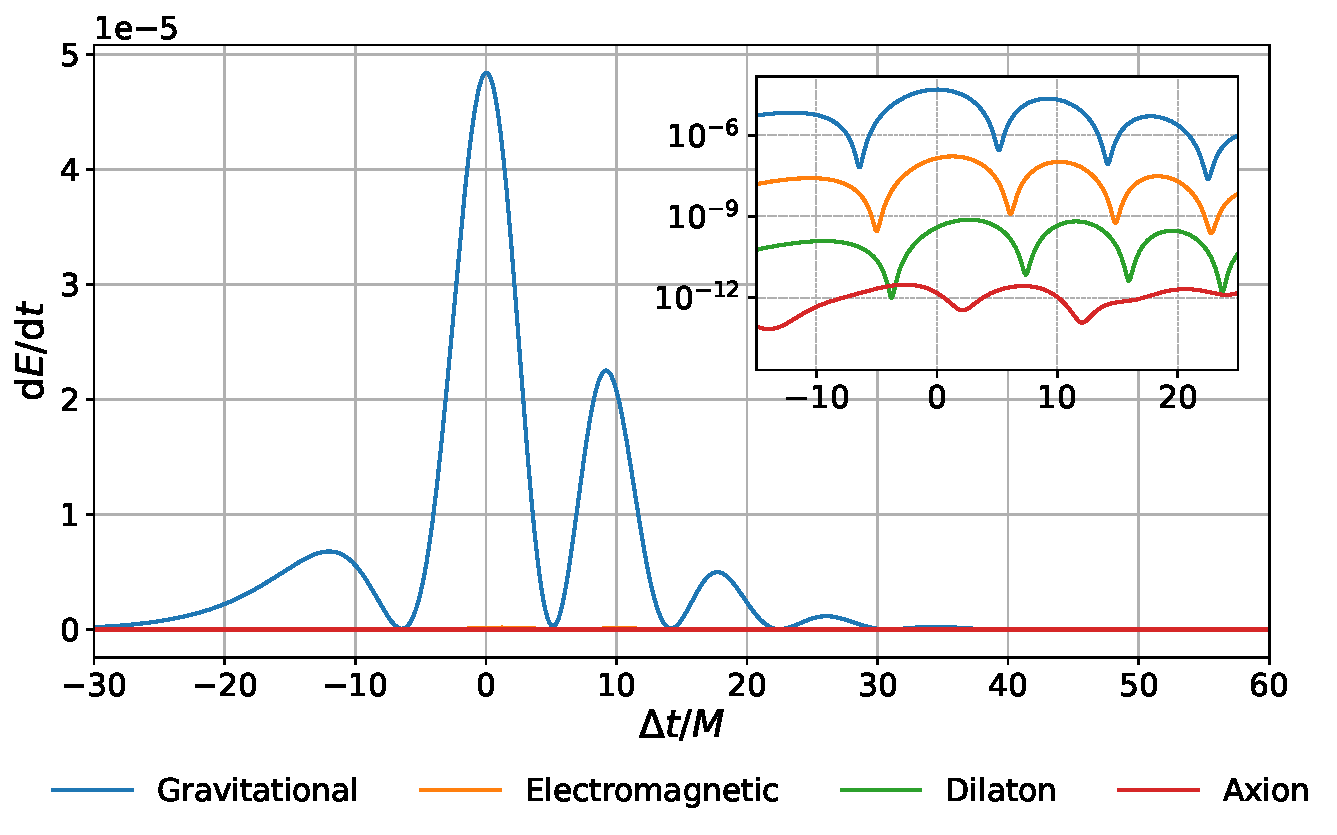
\includegraphics[width=\linewidth]{Figures/Chapter_1/combined_flux_linear_with_inset.pdf}
  \caption{Plot of the radiated energy for the case $\chi = 0.4$ and $q_i/m_i = 0.1$.  The curves have been aligned such that $t = 0$ corresponds to the global maximum. On this plot the axion and dilaton radiation energy remain at least 3 orders of magnitude smaller than the GW or EM contributions}
  \label{fig:flux_chi02_Q05}
\end{figure}



% -------- Scalar field profiles (stacked top to bottom) --------
\begin{figure}[!htbp]
  \centering

  \subfloat[Axion\label{fig:axion}]{
    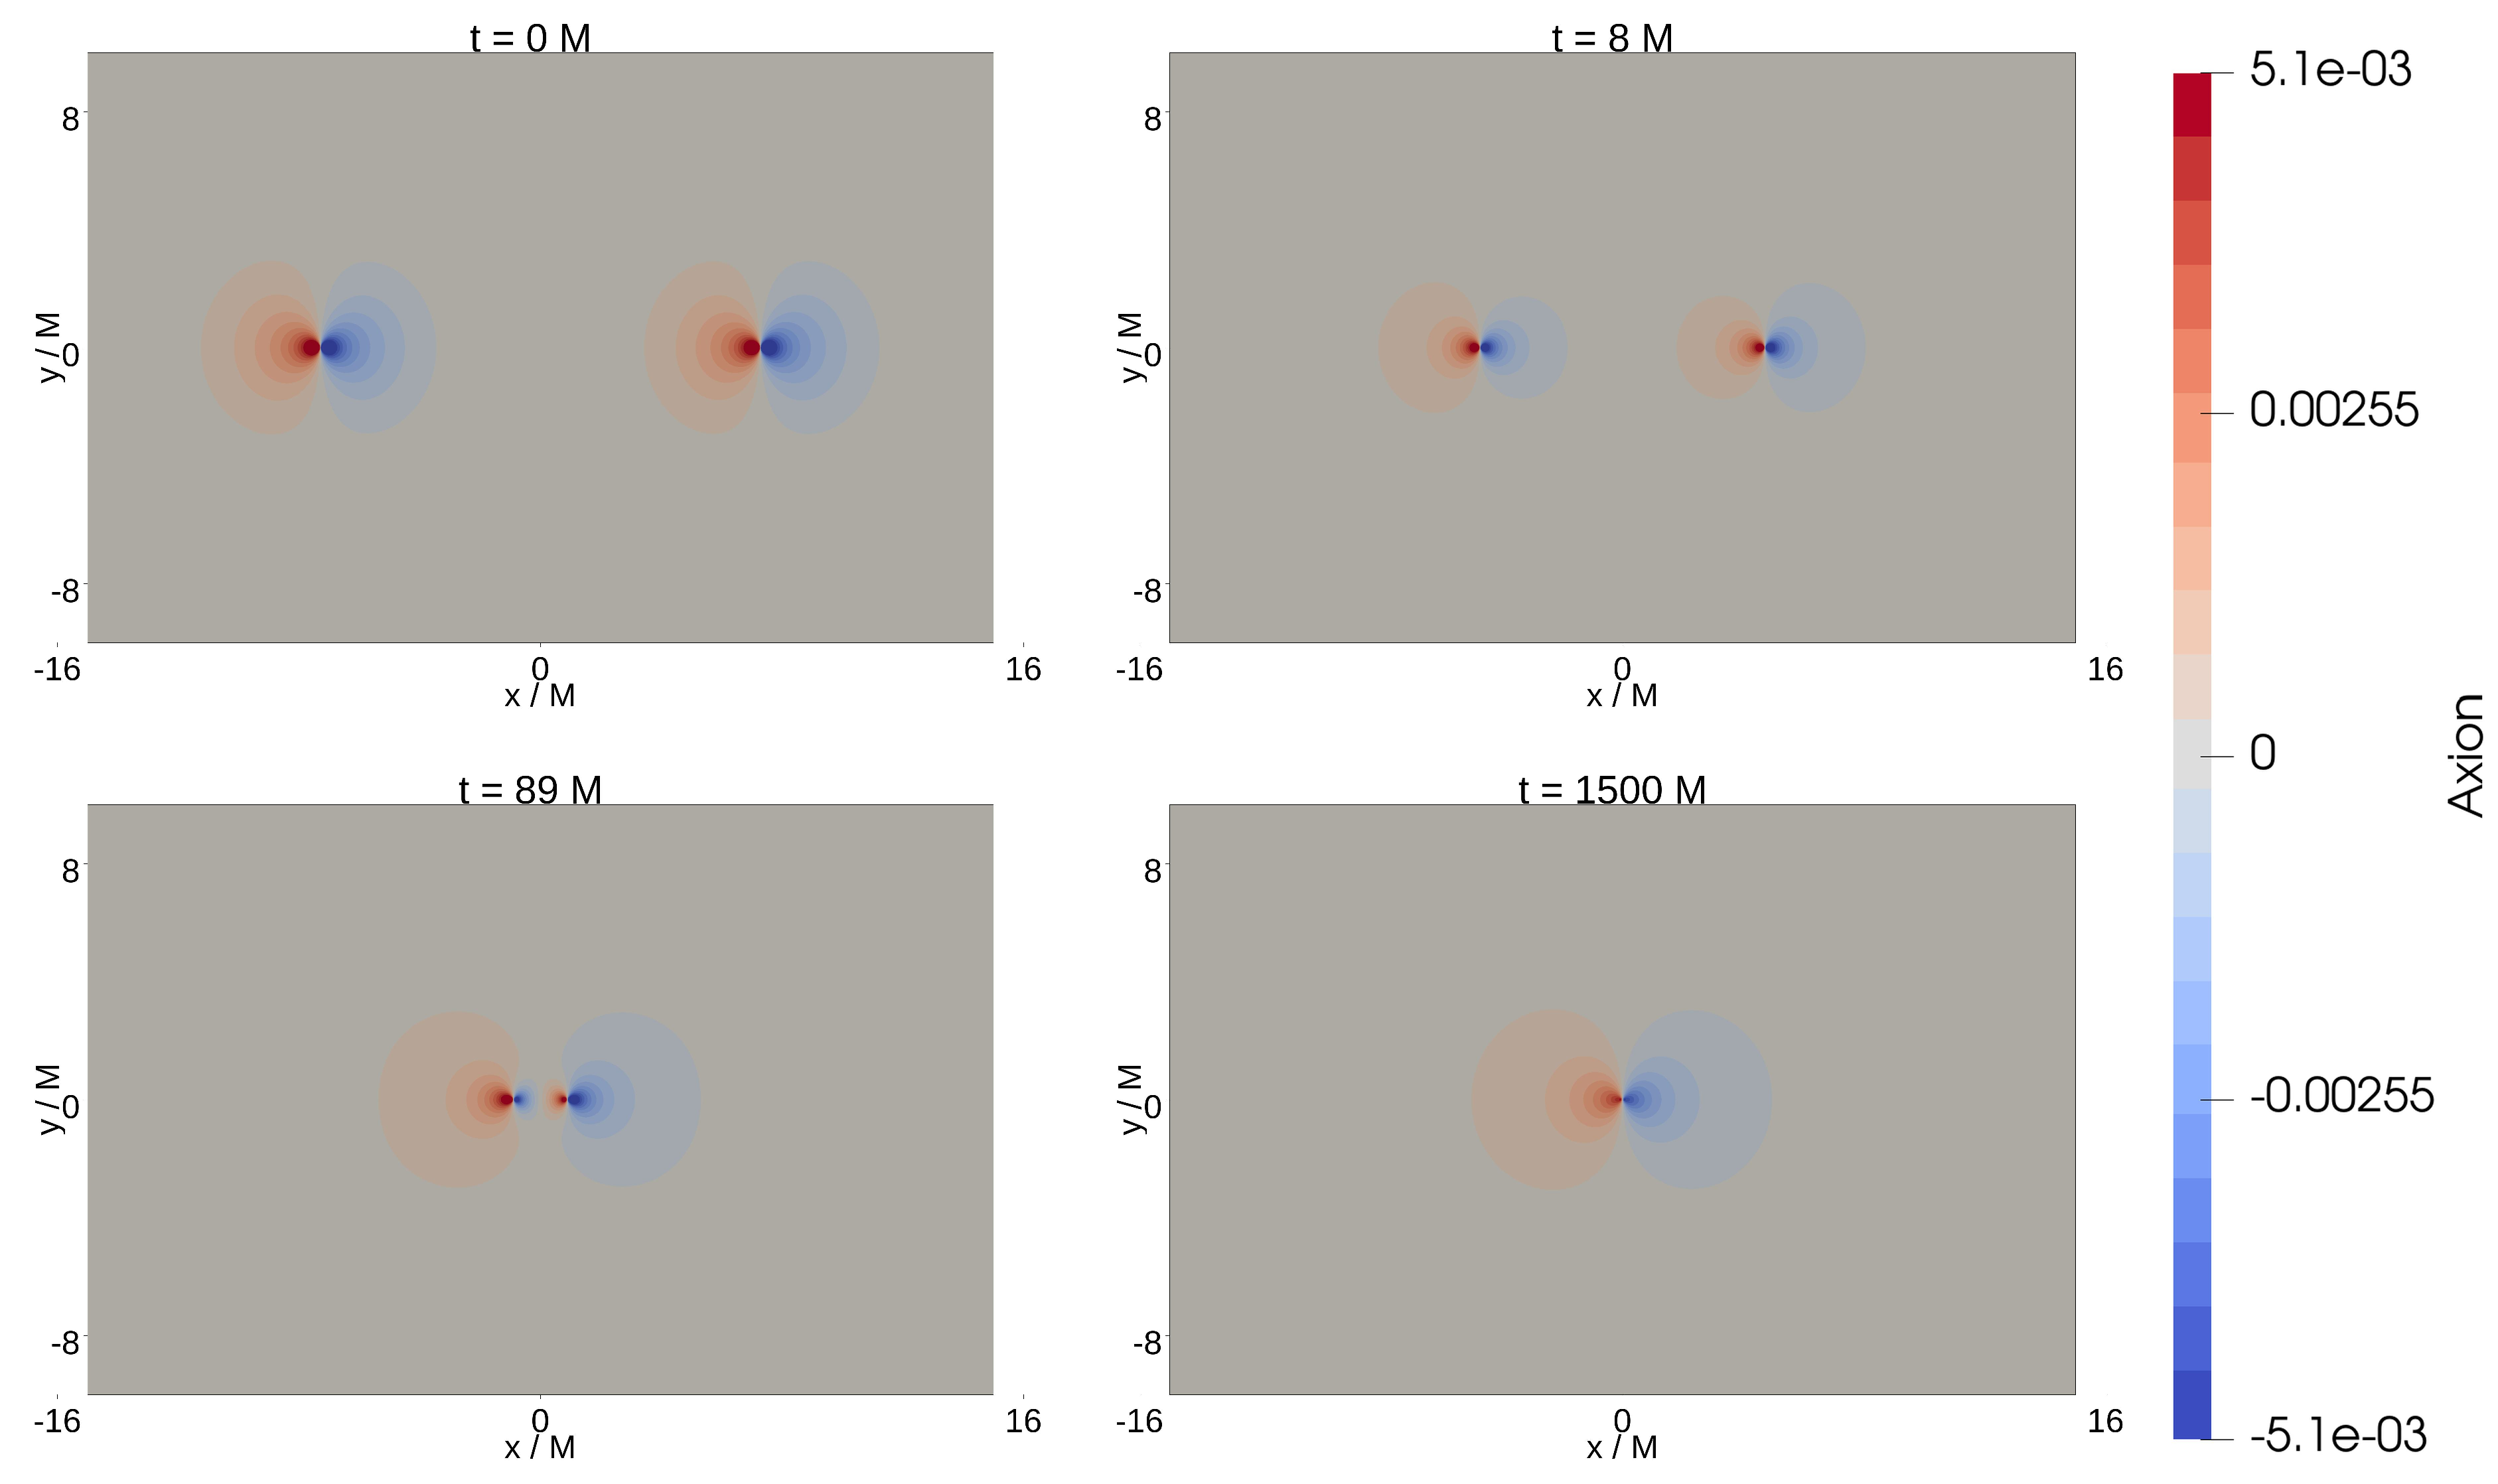
\includegraphics[width=0.92\linewidth]{Figures/Chapter_1/Axion_panel.pdf}
  }\\[0.5em]

  \subfloat[Dilaton\label{fig:dilaton}]{
    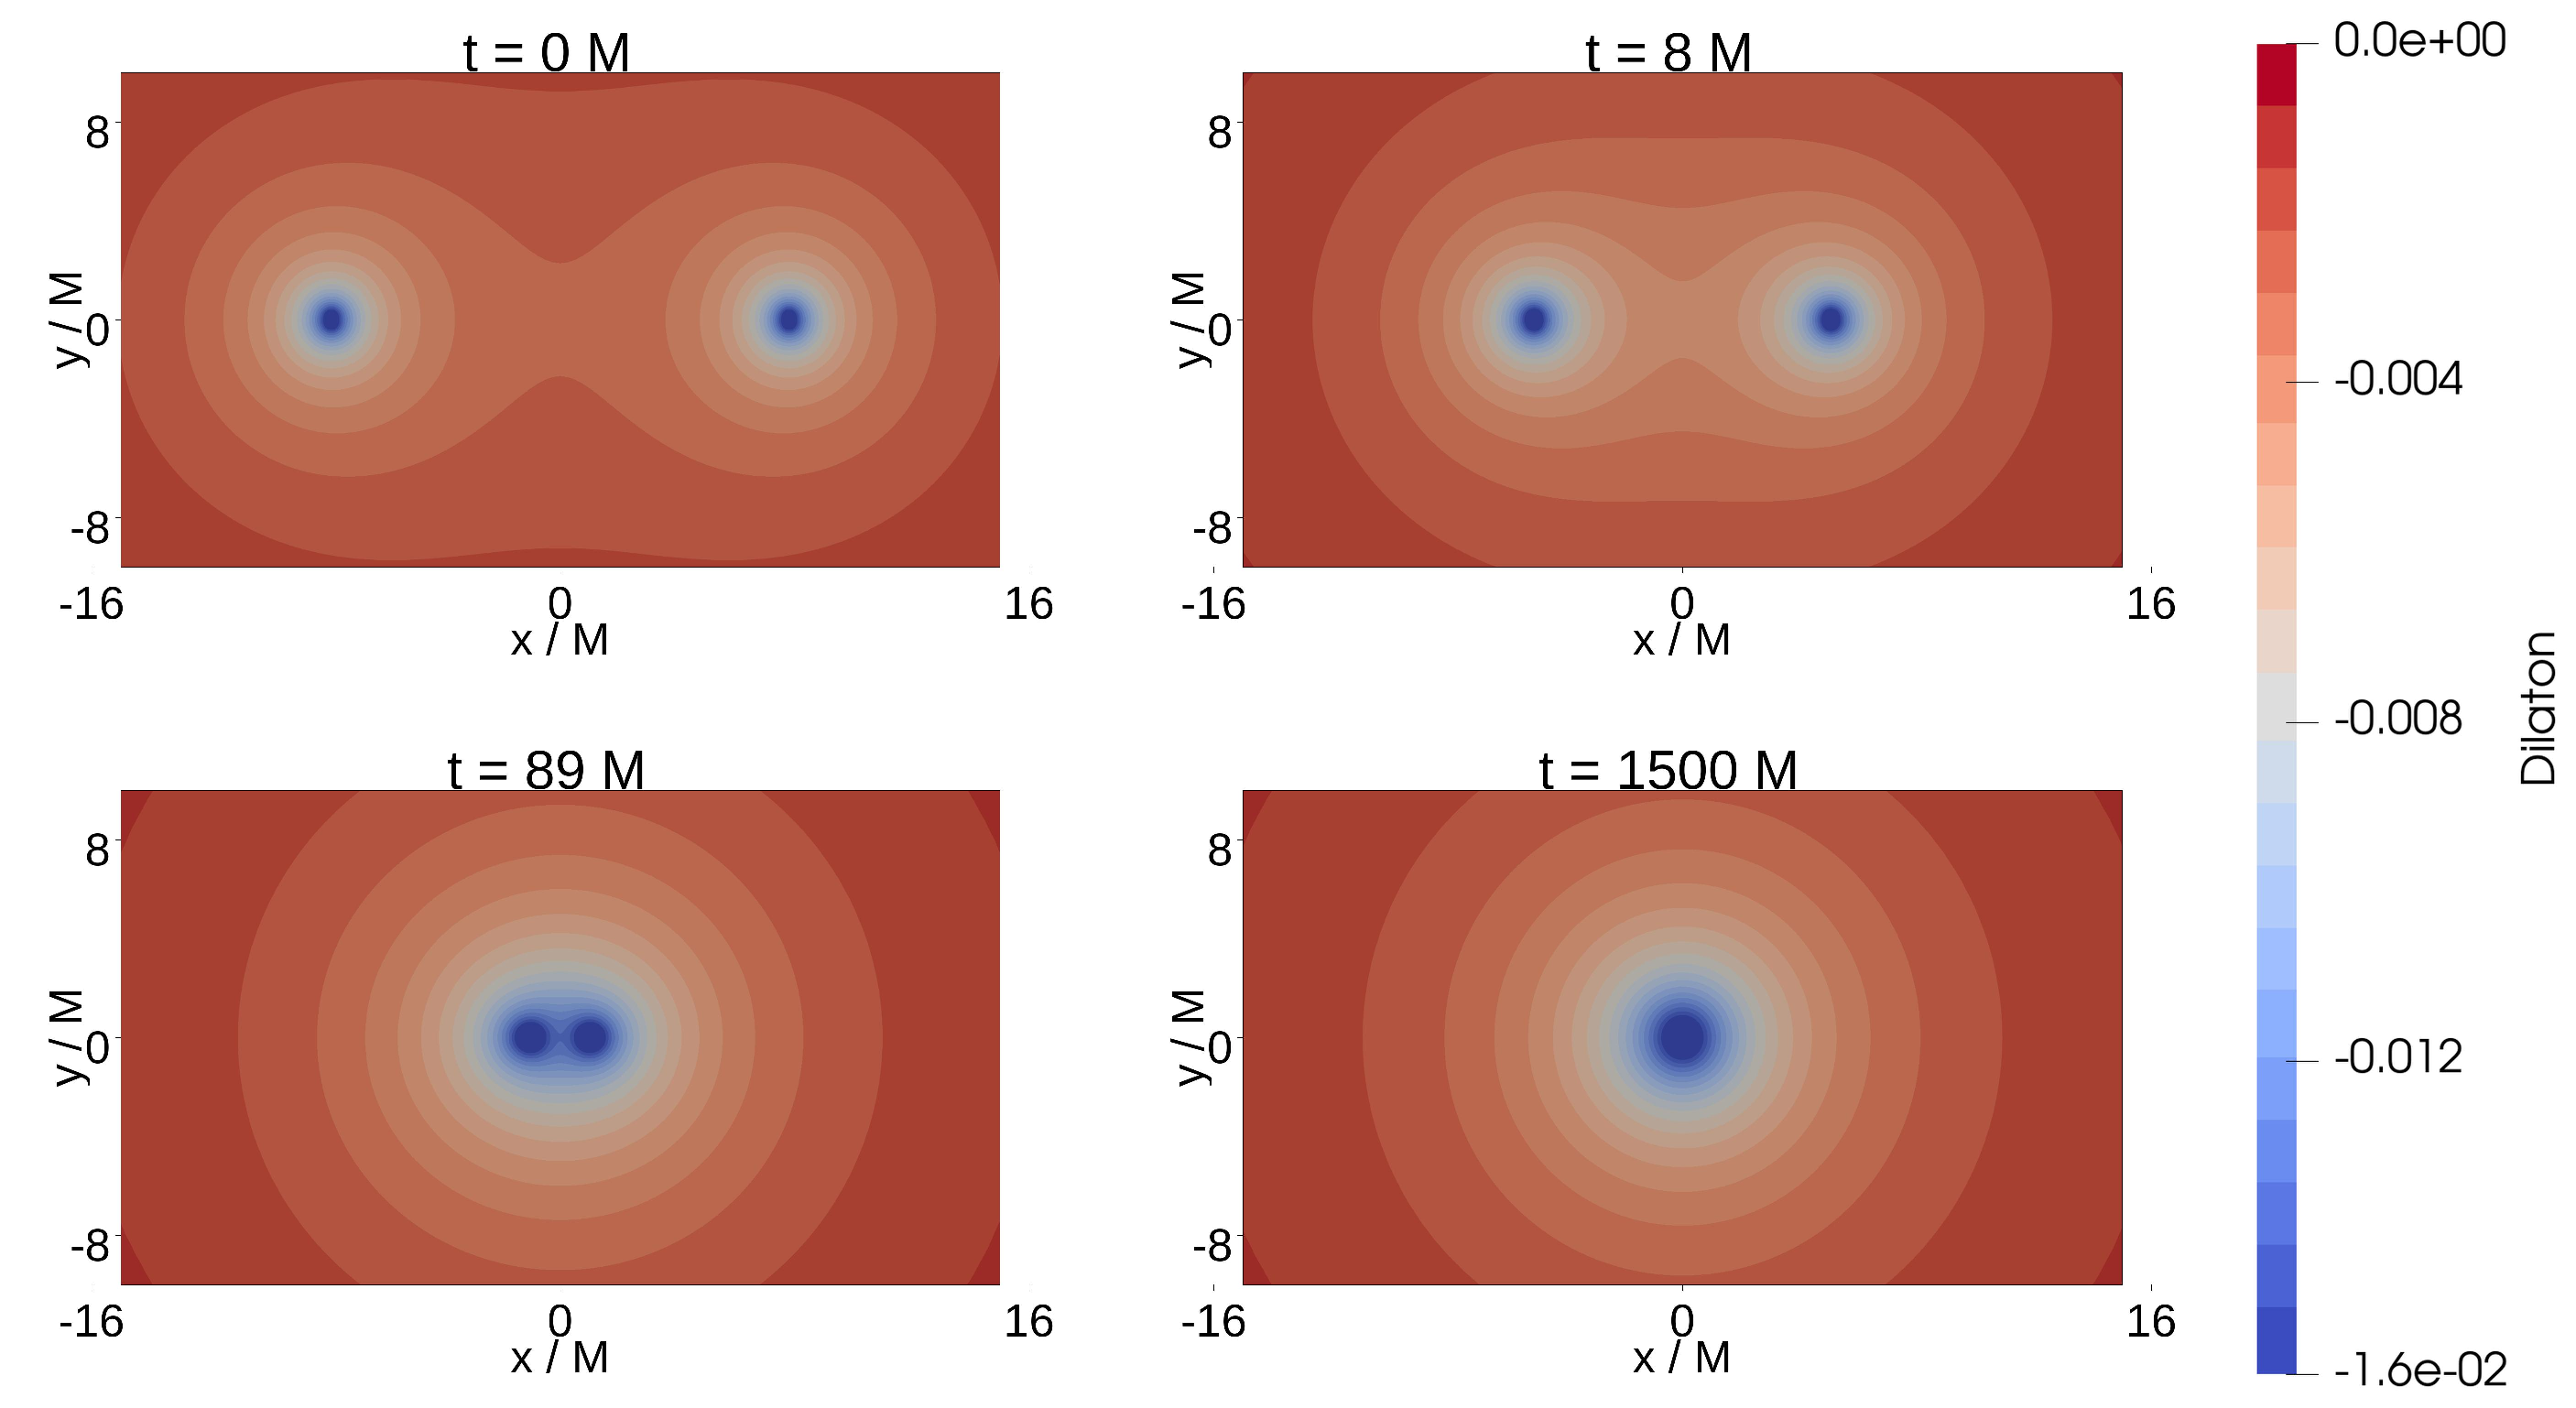
\includegraphics[width=0.92\linewidth]{Figures/Chapter_1/Dilaton_panel.pdf}
  }

  \caption{Scalar fields on the $z=0$ plane for the case $\chi = 0.4$ and $q_i/m_i = 0.1$ Kerr--Sen black holes. We show the amplitudes of the axion, $\kappa$ (top four panels), and dilaton, $\phi$ (bottom four panels), fields at the beginning of the evolution (top left), shortly before merger (top right), just after merger (bottom left), and at a later time after merger (bottom right).}
  \label{fig:scalar_fields}
\end{figure}


% ---------------------------------------------------------
% Remnant black hole quasilocal quantities
% ---------------------------------------------------------

\begin{figure}[!htbp]
  \centering
  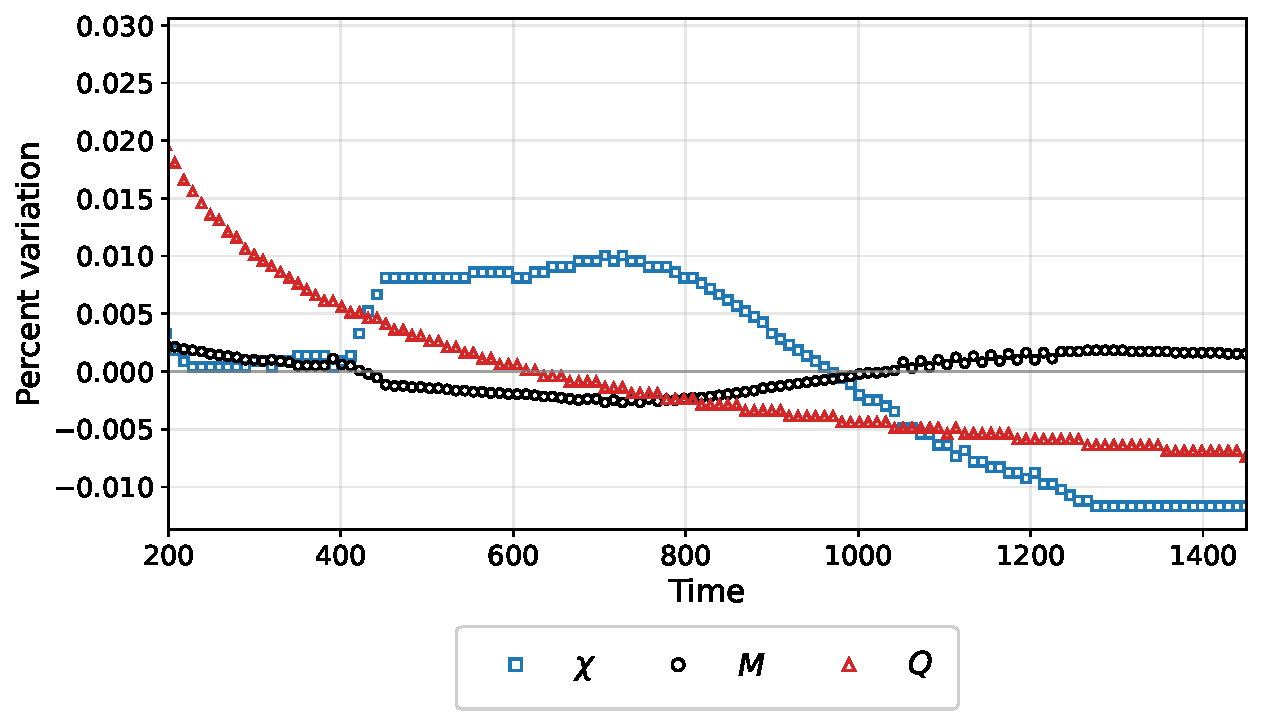
\includegraphics[width=0.92\linewidth]{Figures/Chapter_1/H2_chi_mass_charge_percent_variation.pdf}
  \caption{
  Percent deviation of the remnant black hole's horizon mass $M$, electric
  charge $Q$, and dimensionless spin $\chi$ from their calculated average values:
  $\langle M \rangle = 0.9682$, $\langle Q \rangle = 0.2001$, and
  $\langle \chi \rangle = 0.1961$. These quantities are measured on the
  apparent horizon of the remnant black hole for an initially spinning and
  charged binary black hole configuration with individual charge to mass ratios
  $q_i/m_i = 0.1$, initial dimensionless spins $\chi = 0.4$, and total mass
  $M = 1$.
  }
  \label{fig:ql_m_q_Jz}
\end{figure}

\subsection{Initially Unscalarized Black Holes}

To further assess the stability of scalar hair, we conducted a series of tests initialized with a Gaussian distribution of axion and dilaton fields centered at the origin, with amplitudes ranging from $10^{-7}$ up to almost $10^{-2}$. 
Despite not strictly satisfying the constraints, these superposed perturbative scalar fields propagate outward and enable us to examine whether initially unscalarized black holes can dynamically acquire and retain scalar fields. Our results confirm that they do: a Kerr–Newman black hole in EMDA rapidly scalarizes, developing both dilaton and axion hair. In addition, the change to the constraint violations both from the initial perturbations as well as through the subsequent evolution are small enough to leave us confident in our results.  

Even in the absence of any initial scalar fields in the background, the system evolves to generate nontrivial scalar structure. This demonstrates that scalarization occurs dynamically and does not require pre existing scalar hair. The scalarization occurs quickly with initially Kerr--Newman BHs acquiring Kerr--Sen aspects, i.e. scalar hair prior to merger.  Mass and electromagnetic charge get radiated with a very small amount of scalar hair, but the final object is a Kerr--Sen BH.  
%The conserved quantities, including the total mass and charge, remain effectively constant throughout the evolution. Variations in the conserved quantities over the course of the evolution in both mass and charge are below \(0.2\,\%\). This suggests that these quantities remain stable and conserved over time. 
Figure~\ref{fig:unscalarized} illustrates the evolution of the scalar fields for the case without initial scalar hair on the BHs.

% -------- Scalar field profiles (stacked top to bottom) --------
\begin{figure}[!htbp]
  \centering

  \subfloat[Axion\label{fig:unscalarized_axion}]{
    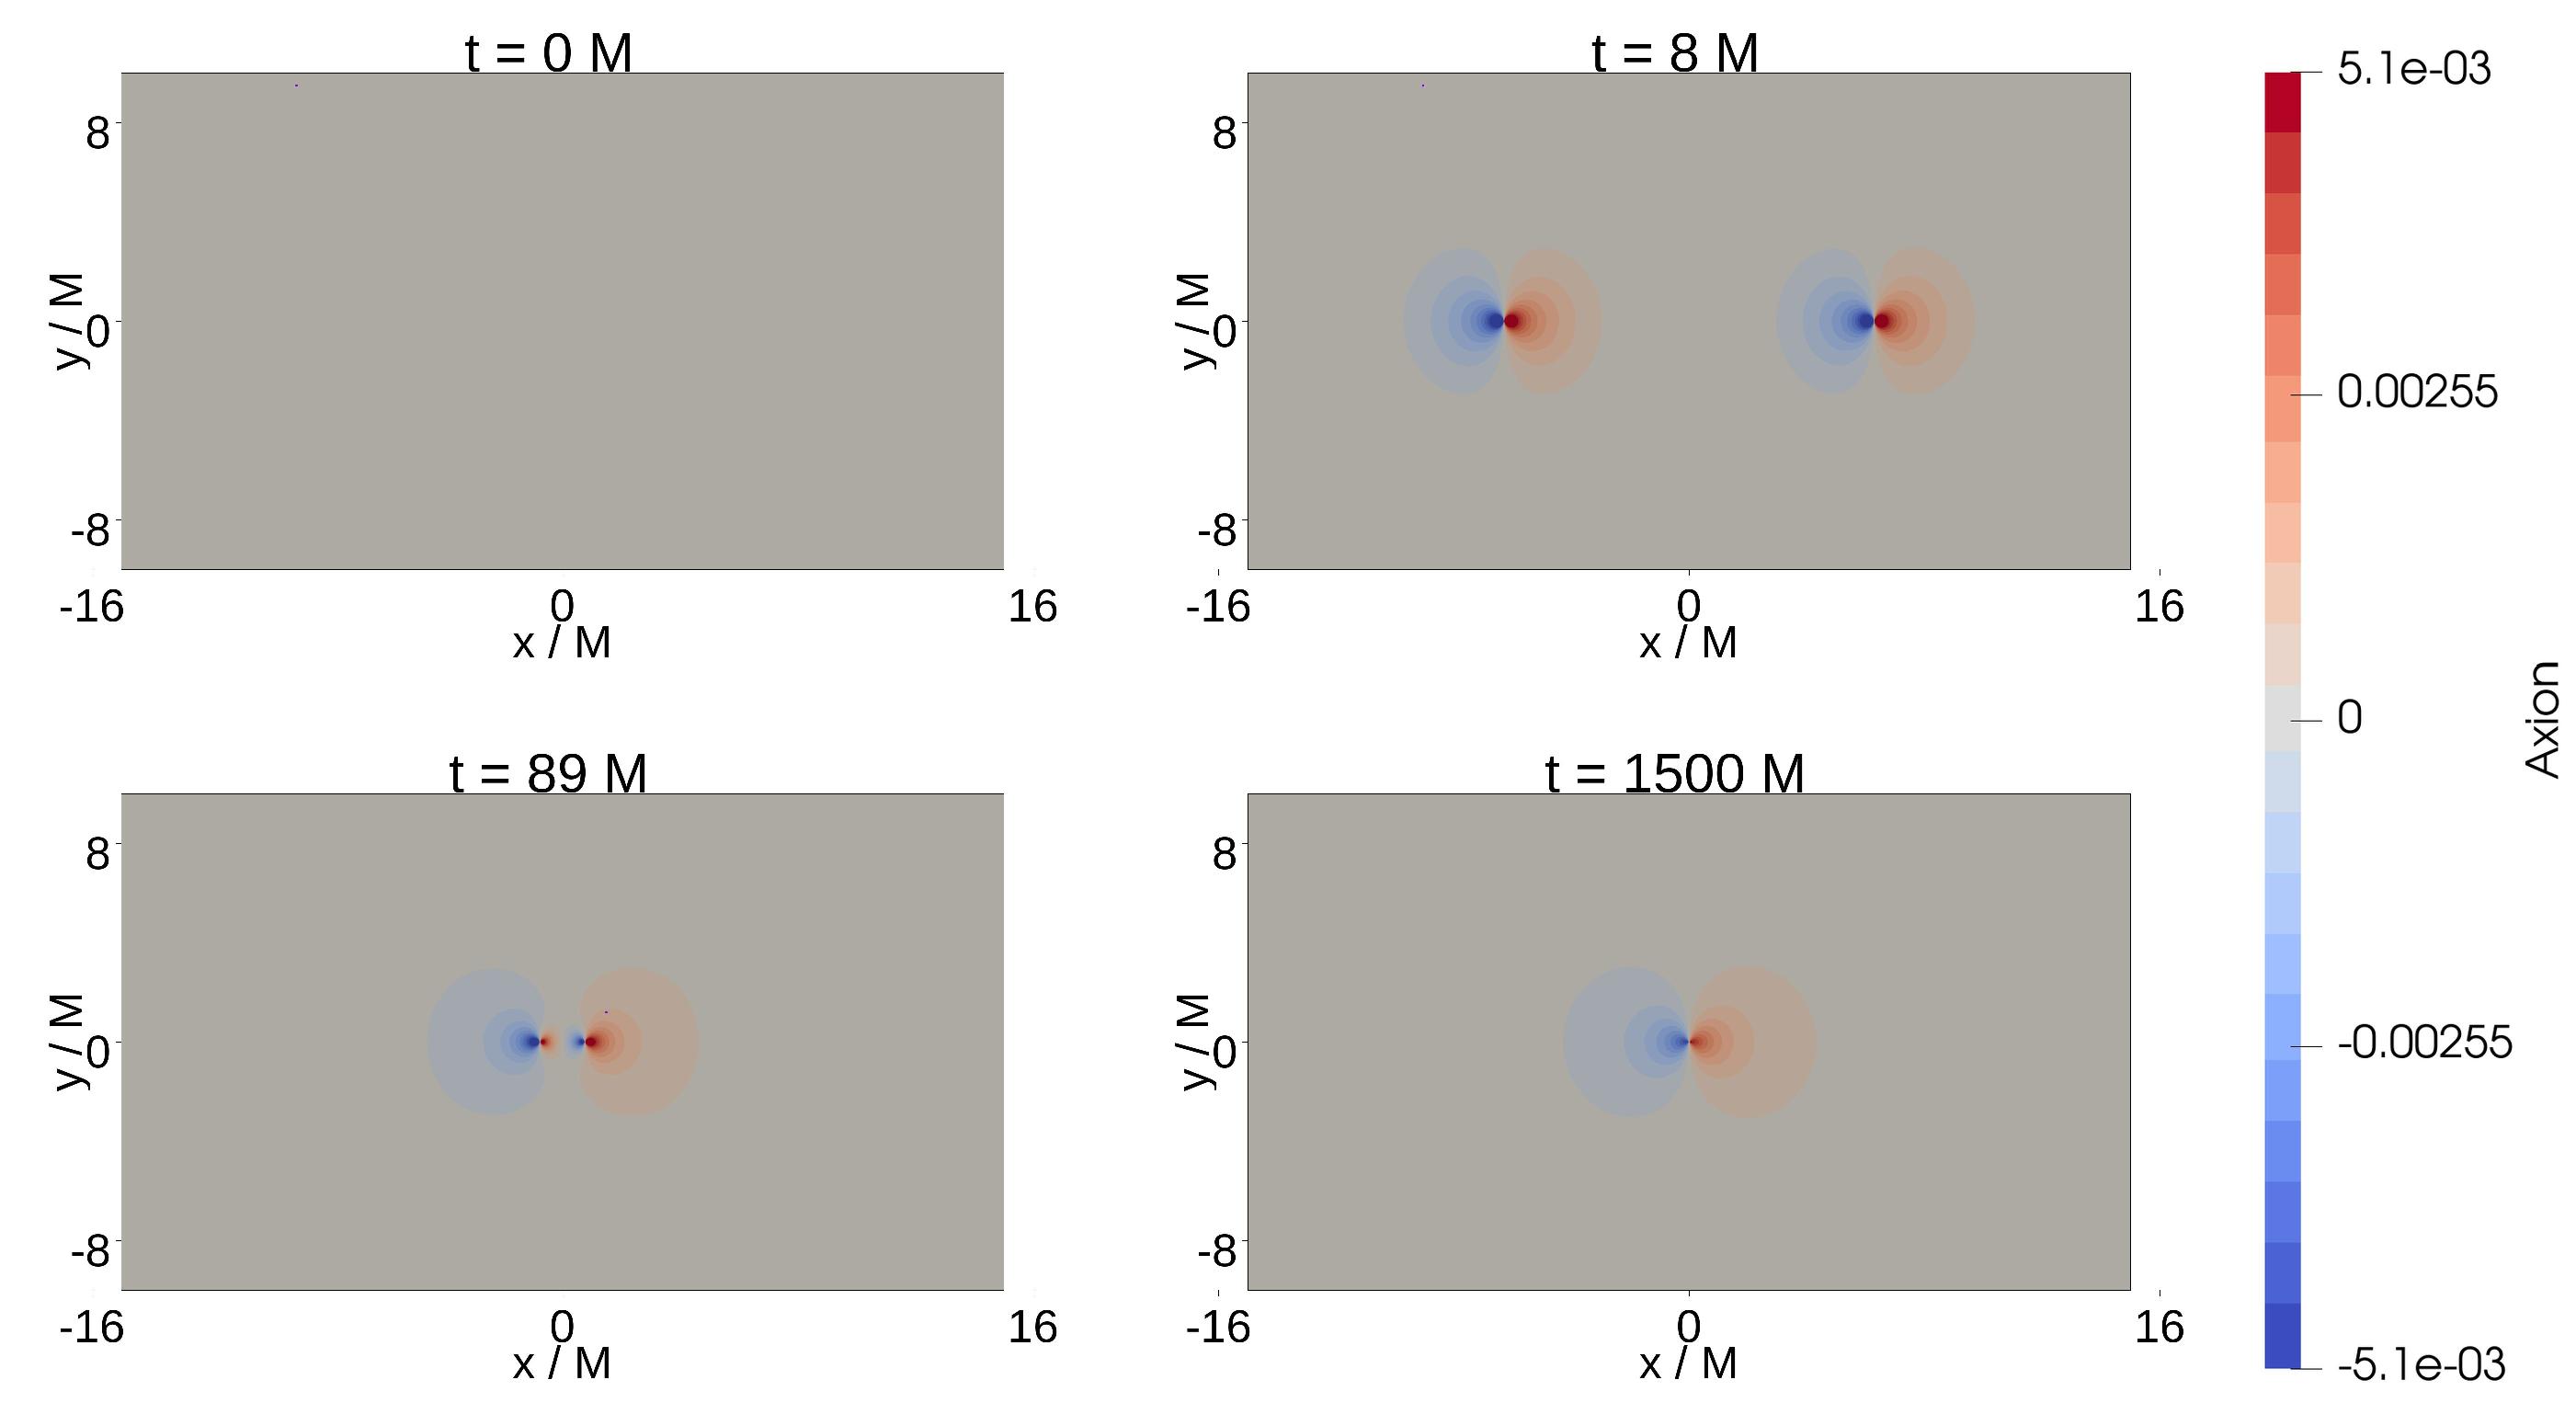
\includegraphics[width=0.92\linewidth]{Figures/Chapter_1/scalar_kappa.pdf}
  }\\[0.5em]

  \subfloat[Dilaton\label{fig:unscalarized_dilaton}]{
    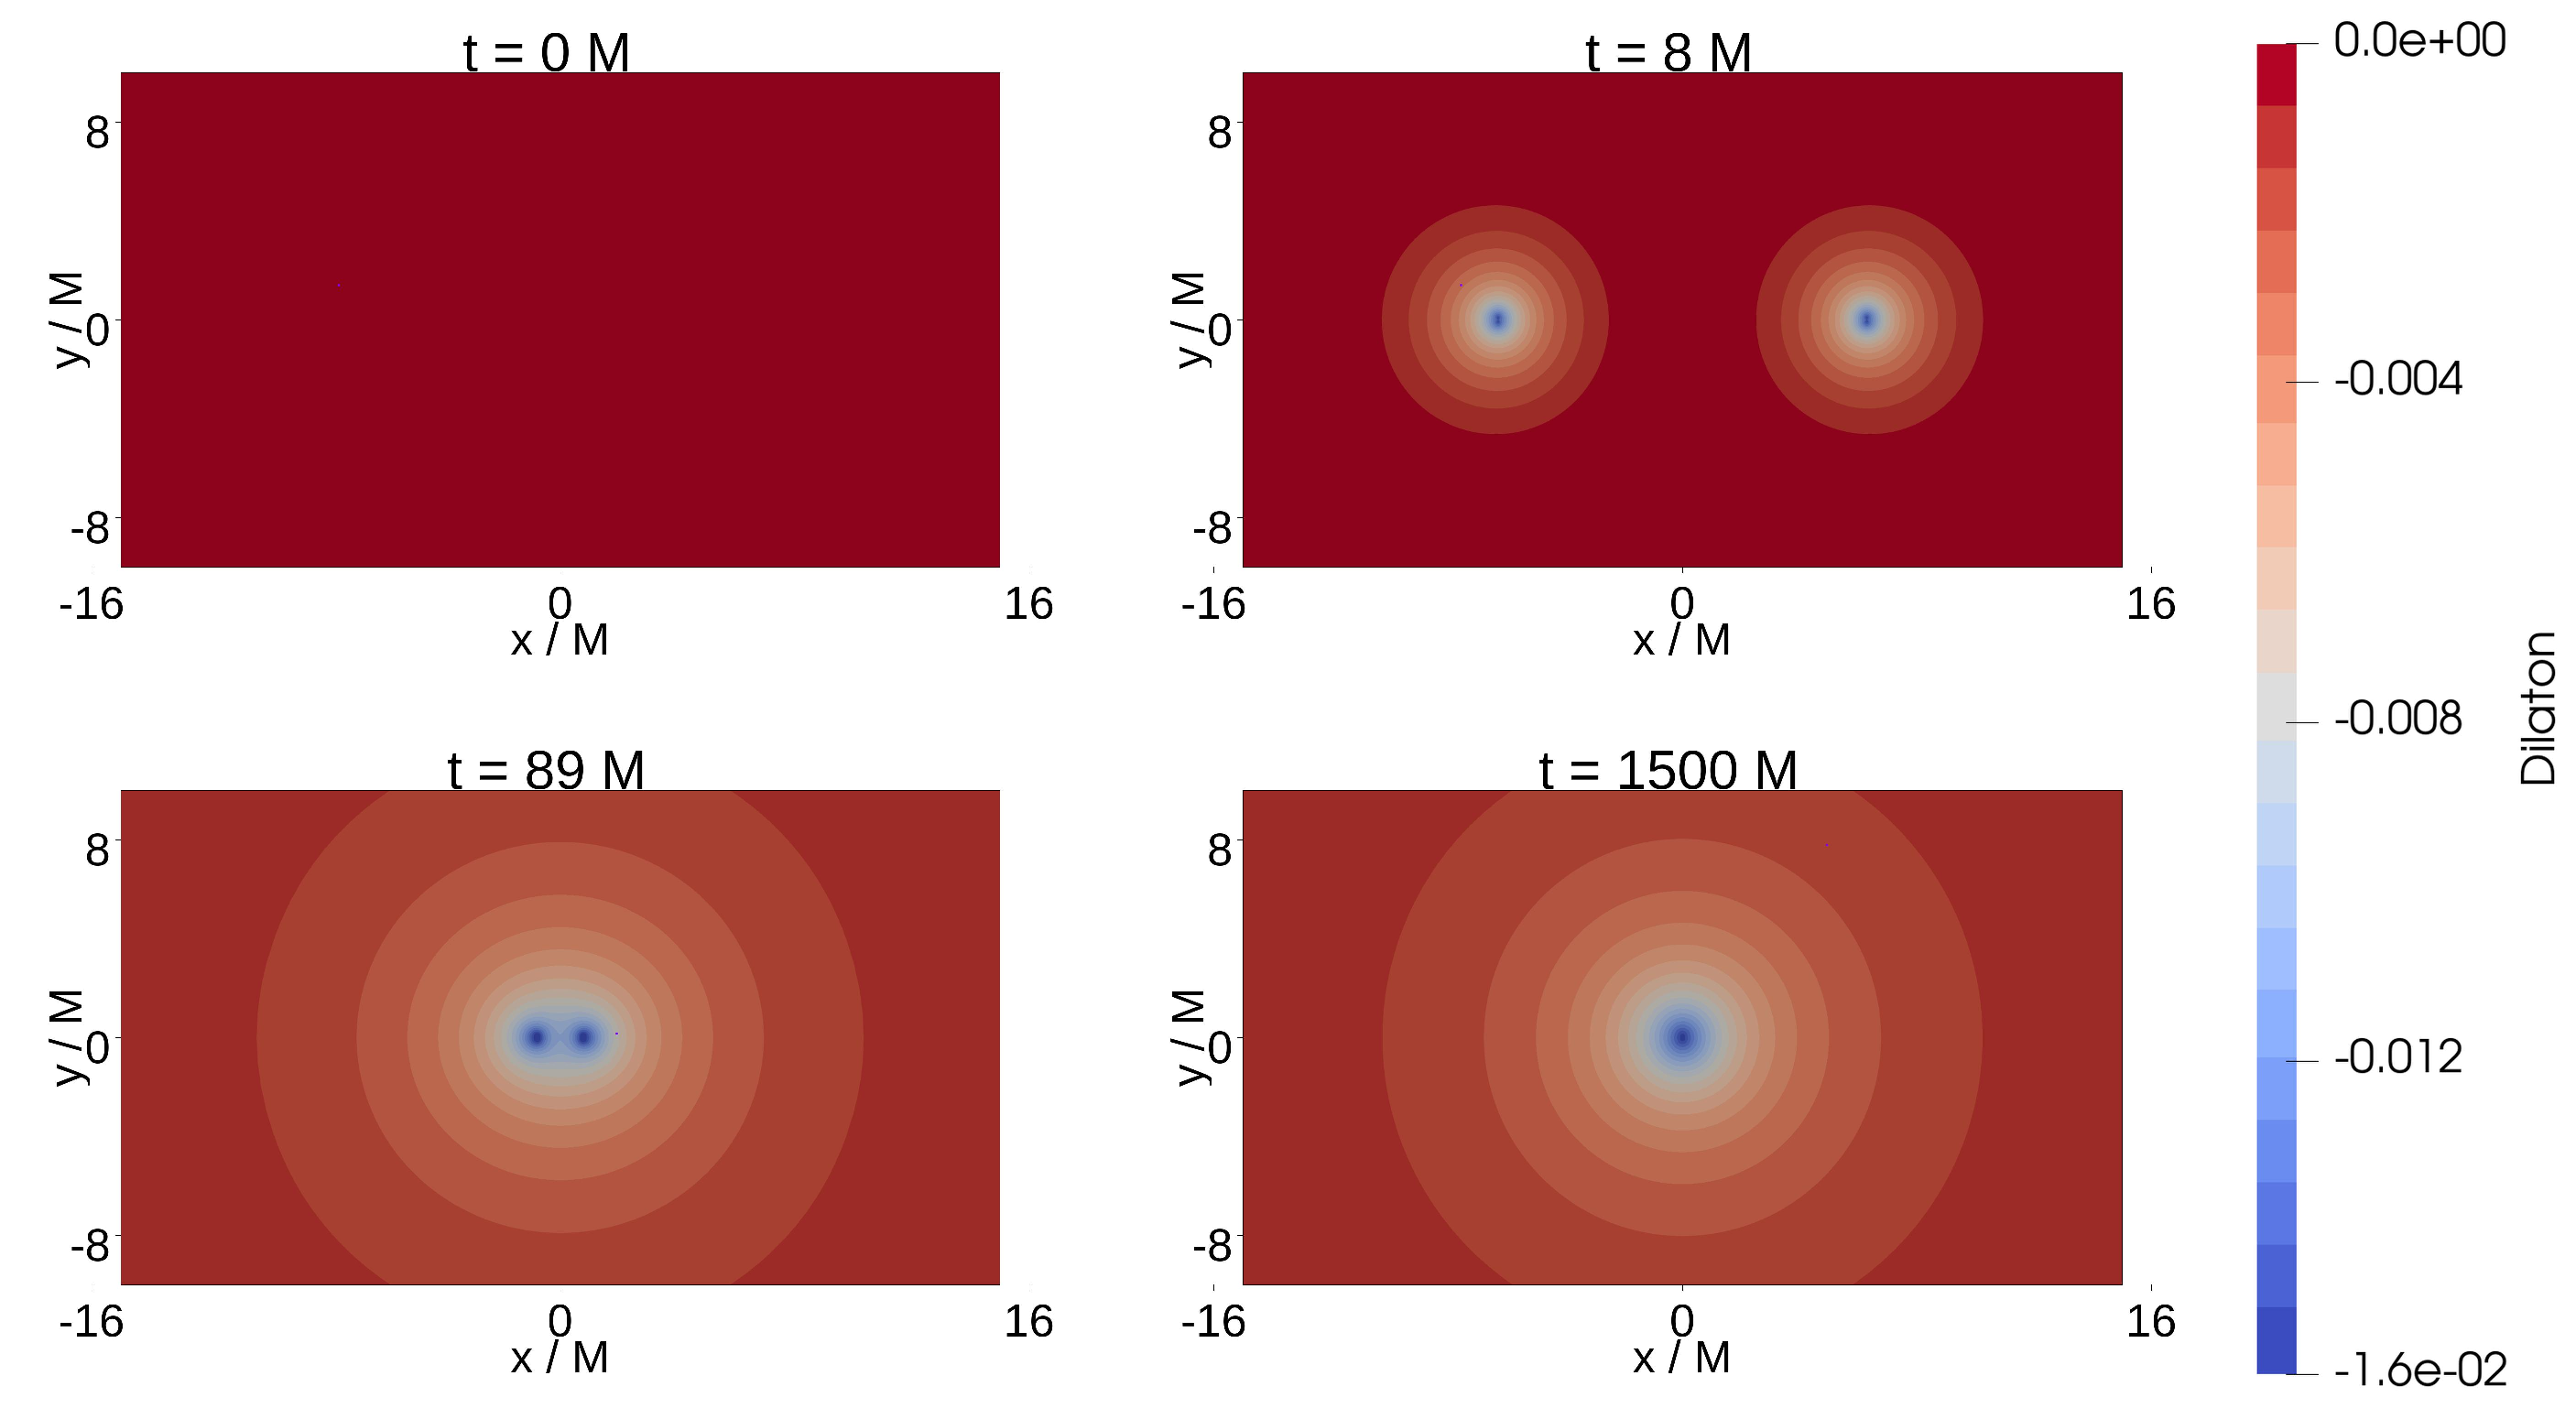
\includegraphics[width=0.92\linewidth]{Figures/Chapter_1/scalar-dil.pdf}
  }

  \caption{Scalar fields on the $z=0$ plane for Kerr--Newman black holes with
  initial dimensionless spin $\chi = 0.4$ and charge to mass ratio
  $q_i/m_i = 0.1$. Initially, neither black hole carries dilaton or axion
  hair. Shown are the amplitudes of the scalar fields $\kappa$ and $\phi$
  at various stages of the evolution: the initial stage (top left), where
  both fields begin at zero; a short time later as the fields start to
  develop (top right); just before merger (bottom left); and some time after
  merger (bottom right).}
  \label{fig:unscalarized}
\end{figure}

\subsection{Constraint and refinement tests}
\label{sec:numerical_diagnostics}

As a consistency check on the evolutions, we monitor the constraint
violations throughout the simulations. Representative full evolution
constraint plots are shown in Appendix~\ref{sec:code_performance}. These
diagnostics show that the Hamiltonian, momentum, and electromagnetic
constraint violations remain controlled over the time scales considered
here, including through the merger and ringdown.

We also perform a limited refinement study for a short head on binary
evolution.  In this study, we vary both the wavelet tolerance and the maximum number of refinement levels.  Both are WAMR related parameters that help dictate the amount and extent of refinement.  The wavelet tolerance is varied between $3\times10^{-5}$ and $3\times10^{-6}$,  
and we consider a maximum number of refinement levels between 14 and 17, corresponding to grid spacings between $h_{14}=0.0325$ and $h_{17}=0.00407$.  
Additional details are given in
Appendix~\ref{sec:code_performance}. Tightening the refinement criteria
reduces the volume weighted Hamiltonian and momentum constraint violations,
consistent with the expected behavior of the WAMR refinement scheme. Taken
together, the full evolution constraint monitoring and refinement tests
indicate that the simulations remain well behaved over the time scales
considered here.


\section{Conclusion}
\label{sec:conclusion}
We have simulated a range of different parameters for the head on collision of Kerr--Sen black holes. We have primarily been concerned with the persistence of scalar hair through this highly nonlinear, dynamical process.  
In summary, our simulations show that the scalar fields do not radiate away so long as there is a nonzero charge (and spin for the axion). We have found that Kerr--Sen black holes are stable. In particular, we find that if the remnant black hole has a nonzero charge, the dilaton field persists. If it has both nonzero charge and spin, the axion field also persists after merger. These results suggest that Kerr--Sen black holes are stable under the conditions and time frames we considered.  

A natural follow up study would be the analysis of waveforms produced by inspiraling black holes, an area where the available results remain relatively limited. Further, while we have assumed a particular member of the family of EMDA theories in this work, namely a low energy limit of heterotic string theory, there is a much larger theory space parametrized by the dilaton and axion couplings, $\alpha_0$ and $\alpha_1$, that remains largely unexplored. A more detailed investigation of this theory space could be intriguing; possibly giving rise to broader classes of stable black holes as well as detectable departures from the predicted general relativistic gravitational wave signal.  
 

% \begin{acknowledgments}
% We would like to thank several individuals for their help and contributions to this work: Gabriele Bozzola for several useful discussions and for sharing his two charged puncture code with us; Zach Etienne for help with \texttt{BHaHAHA}; Milinda Fernando for his extensive insights on the \texttt{Dendro} framework; William Black for many discussions and improvements to \texttt{Dendro GR}.  In addition, thanks to Luis Lehner, Steven Liebling and Carlos Palenzuela for early work on EMD. This research was supported by NSF grant PHY-2207615 (BYU). HL is supported by the LANL ASC program. LANL is operated by Triad National Security, LLC, for the National Nuclear Security Administration of the U.S. DOE (Contract No.~89233218CNA000001). This work is authorized for unlimited release under LA UR-25-31225.

% \medskip
% \noindent\textit{Artificial intelligence assistance.}
% The authors acknowledge the limited use of artificial intelligence tools,
% including ChatGPT and Gemini, during the preparation of this manuscript.
% These tools were used for spelling and grammar checks, LaTeX editing and
% debugging, and improving the clarity and readability of some text. They
% were also used to assist with code debugging and code development. The
% authors reviewed and verified all AI assisted material and take full
% responsibility for the scientific content, calculations, code,
% interpretations, and conclusions presented in this work.
% \end{acknowledgments}




\chapter{Inspiraling Binary Black Hole Waveforms in EMDA Theory}
\section{Introduction}

Gravitational wave observations now provide direct access to the strong-field, dynamical regime of compact-binary coalescence. As detector sensitivities improve and high-signal-to-noise-ratio detections become more likely, the late inspiral, merger, and ringdown will offer increasingly stringent tests of the general-relativistic description of black holes \cite{Abbott2025GWTC3GR,Yunes2025GWTests,Yagi2016_BHTestsGR,Berti2015,Abac2025GW250114}. Recent detections have reached signal-to-noise ratios as high as $80$, enabling tests of Hawking's area law and improved measurements of the remnant black hole \cite{LVK2025GW250114}. These developments motivate numerical studies of how specific beyond-GR effects could appear in the late-inspiral, merger, and ringdown waveform.

For many alternative theories of gravity, analytic approximations are insufficient near merger, while numerical simulations require a well-posed initial-value formulation, stable gauge choices, and controlled constraint behavior as we mentioned in the prior chapter. Considerable effort has been devoted to developing formulations and approximation schemes that permit nonlinear simulations beyond GR \cite{Cardoso2012NRHEP,Corman2024NonlinearModificationsGR,Afshordi2024BlackHolesInsideOut,Bambi2025Mimickers,Bernard2025GenericEFTGWTests}. Examples include studies of dynamical Chern--Simons gravity \cite{Alexander2009,Okounkova2019}, Einstein-dilaton-Gauss-Bonnet theory \cite{Okounkova:2020rqw,Okounkova2020}, modified gauge choices in Einstein-scalar-Gauss-Bonnet theory \cite{Ripley2020a,Ripley2020b}, the ``fixing the equations'' approach \cite{Cayuso2020}, and auxiliary-field formulations for higher-curvature systems, including quadratic gravity \cite{Held2021,Held2023,Held2025,East2023,Taillte2025}. See also Ref.~\cite{Corman2024} for a more detailed comparison of these approaches.

In this chapter, we focus on Einstein--Maxwell--dilaton--axion (EMDA) theory. EMDA extends Einstein--Maxwell theory by coupling the electromagnetic field to a dilaton and an axion, and it arises as a low-energy limit of heterotic string theory \cite{Sen1992,Sen1995}. The theory admits rotating charged black hole solutions, such as the Kerr--Sen spacetime, which differs from Kerr--Newman by the presence of nontrivial dilaton and axion fields. In the last chapter we investigated the stability of black holes and black hole hair in EMDA theory \cite{PopeRohrerWhiting2025,Carroll2026KerrSenStability}, and black hole shadow studies using Event Horizon Telescope observations have not ruled out Kerr--Sen black holes \cite{Sahoo2024PRD,Sahoo2025}. These features make EMDA a useful setting in which to study how additional matter fields can influence compact-binary dynamics and gravitational radiation.

Charged binary black holes have also been studied in Einstein--Maxwell gravity \cite{Bozzola2019,Zilhao2012,Zilhao2014,Bozzola2021,Bozzola2023ExtremalChargedMergers,Luna2022ChargedBBHKicks}. These simulations show that electromagnetic charge can modify the orbital dynamics, emitted radiation, and recoil of the remnant. In one analysis, the GW150914 signal was found to be compatible with charge-to-mass ratios as large as $Q/M\sim0.3$ ~\cite{Bozzola2021}. These studies demonstrate that charge alone can alter the inspiral, merger, radiation content, and remnant properties. In EMDA theory, charge also sources additional scalar and pseudoscalar fields, so charged binaries provide a natural setting in which to study how electromagnetic and beyond-GR matter jointly affect the gravitational waveform.

The goal of this chapter is to take a step toward an exploratory waveform catalog for charged binary black holes within EMDA. We simulate inspiraling charged binary black holes and compare the resulting gravitational waveforms with neutral general relativistic reference waveforms having the same mass ratio and spin. The cases considered here include charge-to-mass ratios much larger than those expected for astrophysical black holes \cite{Gibbons1975VacuumPolarization,Pan2019BlackHoleDischarge}. Our aim is therefore not to construct immediately realistic astrophysical templates, but to identify regimes in which charge and the additional EMDA fields produce appreciable changes in the binary dynamics and gravitational wave signal.

These comparisons should be interpreted as fixed parameter waveform comparisons rather than as a complete parameter-estimation study. Compact-binary waveforms are highly degenerate, and differences between an EMDA waveform and a GR waveform may be partially mimicked by varying intrinsic binary parameters such as the mass ratio, spins, total mass scale, or eccentricity\cite{Hannam2013MassSpinDegeneracy,Vallisneri2013StealthBias}. Moreover, because the comparisons in this chapter are made against neutral GR rather than charged Einstein--Maxwell binaries, the resulting differences should be understood as the combined effect of charge, modified orbital dynamics, and the additional EMDA fields, rather than as isolated dilaton or axion signatures.

The catalog presented here is therefore intended as an initial step toward a more complete study of EMDA binary black hole phenomenology. In particular, it identifies regions of parameter space where charged EMDA binaries produce appreciable waveform differences relative to neutral GR and motivates future comparisons among neutral GR, Einstein--Maxwell, and EMDA binaries.

\section{Einstein--Maxwell--Dilaton--Axion Theory}
\label{sec:emda}

We consider Einstein--Maxwell--dilaton--axion (EMDA) theory, in which the Einstein--Maxwell system is supplemented by a scalar dilaton field $\phi$ and a pseudoscalar axion field $\kappa$. With the conventions used here, the action is
\begin{equation}
\begin{aligned}
S = \int \mathrm{d}^4 x,\sqrt{-g}\Big[
&\frac{R}{8\pi}
-2\nabla_a\phi\nabla^a\phi
-e^{-2\alpha_0\phi}F_{ab}F^{ab} -\frac{1}{2}e^{4\alpha_1\phi}\nabla_a\kappa\nabla^a\kappa
-\kappa F_{ab}({}^{*}F)^{ab}
\Big],
\end{aligned}
\label{eq:emda_action}
\end{equation}
where $R$ is the Ricci scalar, $F_{ab}$ is the $U(1)$ field strength, and $({}^{*}F)_{ab}$ is its dual. The constants $\alpha_0$ and $\alpha_1$ determine the coupling strengths between the electromagnetic field and the dilaton and axion fields.

As we mentioned in the prior chapter different choices of $\alpha_0$ and $\alpha_1$ correspond to different members of this class of theories. The parameter $\alpha_0$ controls the exponential coupling between the dilaton and the electromagnetic field, while $\alpha_1$ controls the exponential coupling of the dilaton to the axion kinetic term. For example, the choice $(\alpha_0,\alpha_1)=(\sqrt{3},0)$ gives the Kaluza--Klein value of the dilaton coupling \cite{Horne1992,Mignemi1993_ChargedStringBH}. In the simulations presented here, we fix
\begin{equation}
(\alpha_0,\alpha_1)=(1,1),
\end{equation}
which corresponds to the coupling values associated with the low-energy limit of heterotic string theory \cite{Sen1992,Sen1995}.

For this choice of couplings, the theory admits rotating charged black hole solutions of the Kerr--Sen type \cite{Sen1992}. These solutions reduce to Kerr in the limit of vanishing electromagnetic charge, but for nonzero charge the black hole is accompanied by a nontrivial dilaton field and, in the rotating case, a nontrivial axion field. The structure of these fields is known analytically for a single isolated black hole; the solution we summarized in the previous chapter.

To simulate inspiraling binary black holes, we construct approximate charged binary black hole initial data and evolve the full EMDA system numerically. This allows us to compare the resulting gravitational waveforms against neutral general relativistic reference waveforms and to identify how the combined electromagnetic, dilaton, and axion fields influence the inspiral and merger.

\section{Numerical Methods}
\label{sec:methods}

To study the strong-field dynamics and gravitational radiation from inspiraling charged black hole binaries in Einstein--Maxwell--dilaton--axion (EMDA) theory, we evolve the full EMDA system as a Cauchy initial-value problem. The spacetime metric is evolved using the BSSN formulation \cite{Shibata1995_BSSN,Baumgarte1999_BSSN,Baumgarte2010}, together with puncture gauge conditions \cite{Campanelli2006,Baker2006}. The electromagnetic, dilaton, and axion fields are evolved using the matter evolution equations obtained from the $3+1$ decomposition of the EMDA equations of motion. The full evolution system is summarized earlier.

The simulations are initialized with approximate charged binary black hole initial data and evolved through the late inspiral, merger, and ringdown. During the evolution, we extract gravitational radiation and monitor the matter fields, constraints, and quasilocal horizon quantities in order to assess the dynamics and numerical consistency of the solutions.

\subsection{Numerical implementation}
\label{sec:code_description}

For the simulations presented here, we evolve the EMDA system using the same code described in Chapter~2, \texttt{Dendro-GR}. Further details on the \texttt{Dendro-GR} infrastructure, including its adaptive wavelet-refinement strategy, code-generation framework, scalability, and previous applications to binary black hole simulations, can be found in the previous chapter and in Refs.~\cite{Fernando2019,Fernando2019b,Fernando2023,Black2025_ORBIT}. In particular, \texttt{Dendro-GR} has been shown to perform well for intermediate-mass-ratio inspiral simulations, where adaptive refinement is especially useful for resolving disparate length scales \cite{Fernando2019b,Black2025_ORBIT}.

As before, throughout each evolution, we monitor the Hamiltonian and momentum constraints, as well as the electromagnetic divergence constraints. These quantities are used to track the consistency of the numerical solution and to assess whether the chosen refinement parameters adequately resolve the relevant dynamics.

We also extract quasilocal horizon quantities using a modified version of the \texttt{BHaHAHA} apparent-horizon finder \cite{Etienne2026BHaHAHA}. In addition to locating the apparent horizons, this modified version computes the horizon mass, spin, and electric charge during the evolution.
\subsection{Controlling the eccentricity}
\label{sec:eccentricity_control}

In this chapter, we focus on approximately quasicircular inspirals. For uncharged binary black holes, post-Newtonian methods can be used to choose initial momenta that reduce the orbital eccentricity.Post Newtonian methods approximate general relativity by expanding the equations of motion in powers of $v/c$, where $v$ is the characteristic orbital speed. They are most accurate when the objects are moving slowly compared with the speed of light and are separated by distances large compared with their gravitational radii. In compact binary systems, post Newtonian theory provides analytic expressions for the orbital dynamics and gravitational waveform during the inspiral, before the late merger regime where full numerical relativity is needed. In the EMDA system, however, the presence of electromagnetic, dilaton, and axion fields complicates the construction of low-eccentricity initial data. Post-Newtonian treatments have been developed for Einstein--Maxwell theory and for several scalar-modified theories of gravity~\cite{Khalil2018_EMD_EOB,Yagi2012_QuadraticGravityPN,Julie2019_EsGB_PN,Gupta2025_EinsteinMaxwell2PN}. Here we adopt a simpler prescription based on the charged-binary argument used in Ref.~\cite{Bozzola2021}.

At Newtonian order, both the gravitational and electromagnetic interactions are central forces. For two charged compact objects, the Coulomb interaction modifies the effective strength of the attractive force. Denoting the charge-to-mass ratio of each black hole by
\begin{equation}
\lambda_i = \frac{Q_i}{M_i},
\end{equation}
the leading-order effect of the electromagnetic interaction can be incorporated through the replacement of Newton's constant
\begin{equation}
G \rightarrow \tilde{G} = G\left(1-\lambda_1\lambda_2\right).
\end{equation}
In units where $G=1$, this becomes
\begin{equation}
\tilde{G} = 1-\lambda_1\lambda_2 .
\end{equation}
Thus, like-signed charges reduce the effective attraction, while oppositely signed charges increase it. We first compute the momenta required for the corresponding uncharged binary to be approximately quasicircular using post-Newtonian estimates, and then rescale the orbital momenta according to the charge-dependent effective coupling. At leading Newtonian order, this corresponds to scaling the tangential momentum by
\begin{equation}
p_t \rightarrow p_t \sqrt{1-\lambda_1\lambda_2}.
\end{equation}
This prescription assumes that the dominant correction to the initial orbital parameters comes from the electromagnetic interaction; possible direct corrections from the dilaton and axion fields are not included in the initial momentum estimate.

We focus on quasicircular orbits because gravitational wave emission tends to circularize isolated compact binaries during the inspiral \cite{Peters1964,Pfeiffer2007ReducingEccentricity}.The initial momenta for the corresponding uncharged binaries are computed using the \texttt{NRPyPN} package~\cite{Etienne2023_NRPyPN}. This package provides post-Newtonian estimates for low-eccentricity binary black hole initial data compatible with Bowen--York/TwoPunctures data~\cite{Healy2017_PNQuasicircular,RamosBuades2019_EccRed}. We then apply the charge-dependent rescaling described above to obtain the momenta used in the charged evolutions.

Although approximate, this prescription yields eccentricities that are adequate for the exploratory comparisons performed here, as illustrated in Figs.~\ref{fig:orbital_dynamics_q1_q2} and~\ref{fig:orbital_dynamics_q4_q8}. This figure demonstrates that the black hole trajectories are approximately circular. 
\FloatBarrier
\begin{figure}[p]
\centering


\subfloat[$q=1$: black hole separation.\label{fig:bh_separation_q1}]{%
    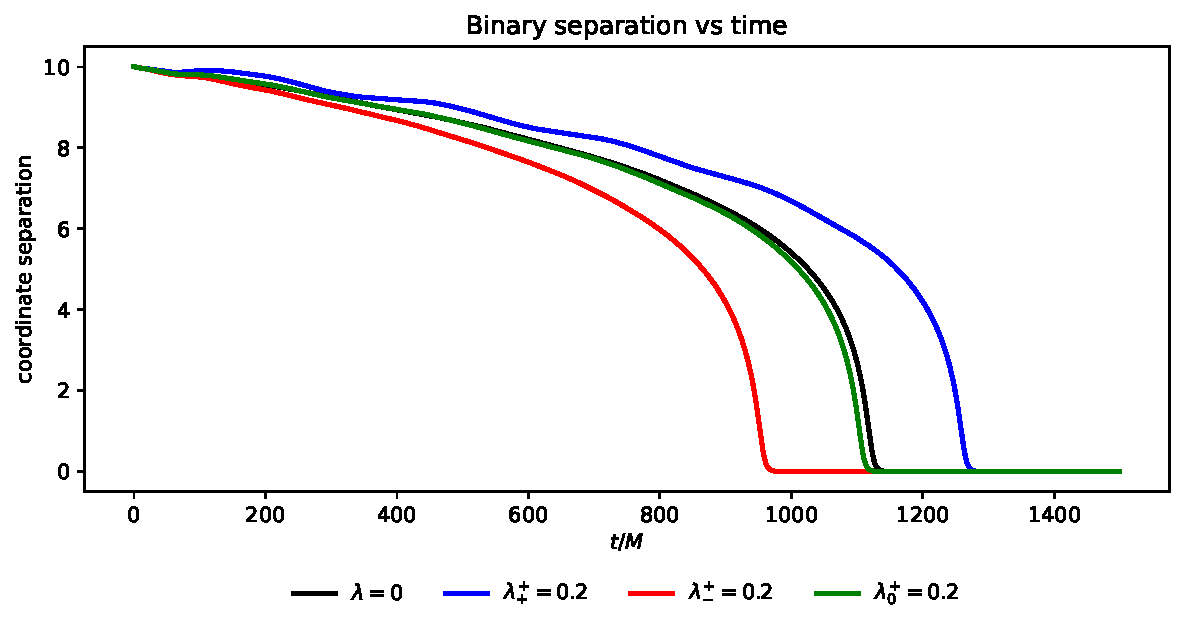
\includegraphics[height=0.22\textheight,keepaspectratio]{Figures/Chapter_2/Q1_SPIN_04_high_charge_separation_comparison.pdf}%
}
\hfill
\subfloat[$q=1$: orbital trajectories.\label{fig:bh_xy_q1}]{%
    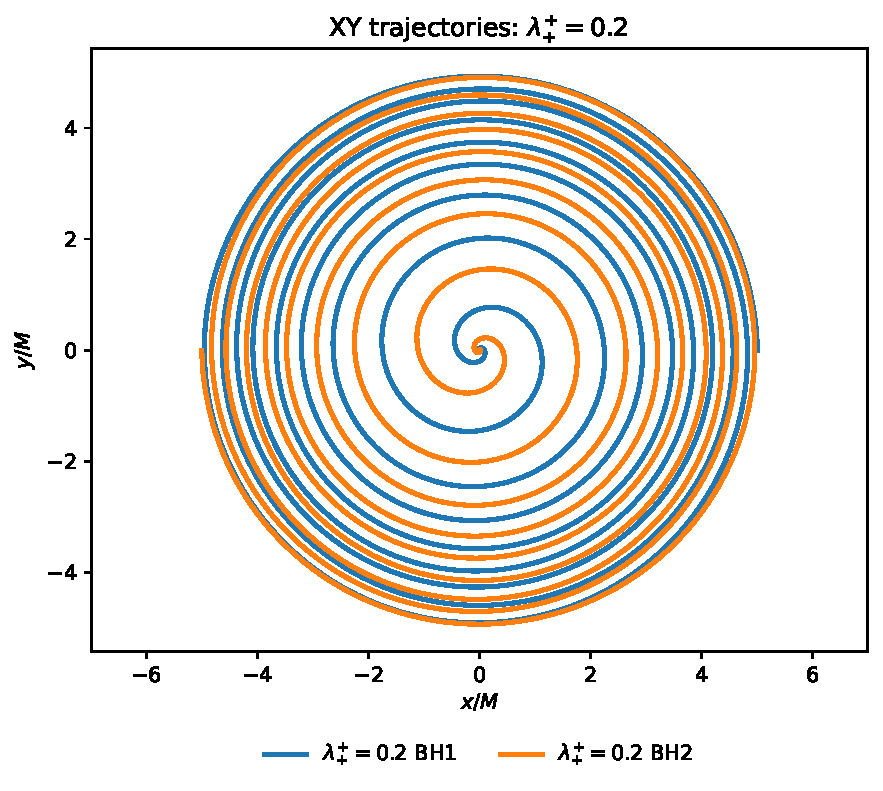
\includegraphics[height=0.22\textheight,keepaspectratio]{Figures/Chapter_2/Q1_SPIN_04_high_charge_Q0p1_pp_xy_trajectory.pdf}%
}

\vspace{1.0em}

\subfloat[$q=2$: black hole separation.\label{fig:bh_separation_q2}]{%
    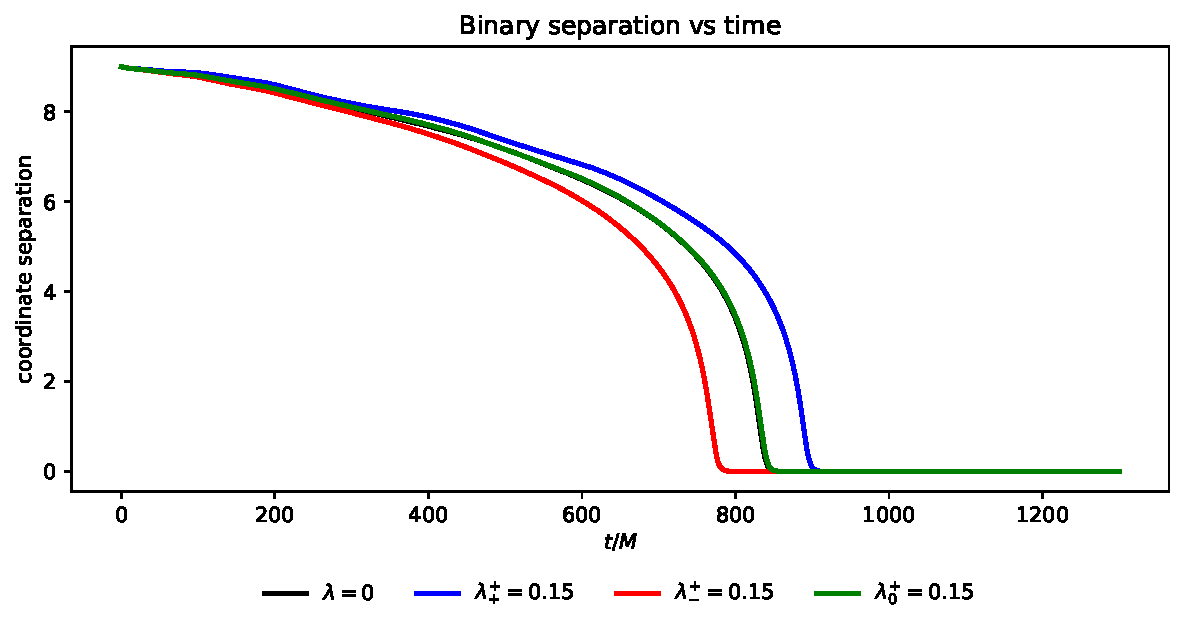
\includegraphics[height=0.22\textheight,keepaspectratio]{Figures/Chapter_2/Q2_SPIN_04_high_charge_separation_comparison.pdf}%
}
\hfill
\subfloat[$q=2$: orbital trajectories.\label{fig:bh_xy_q2}]{%
    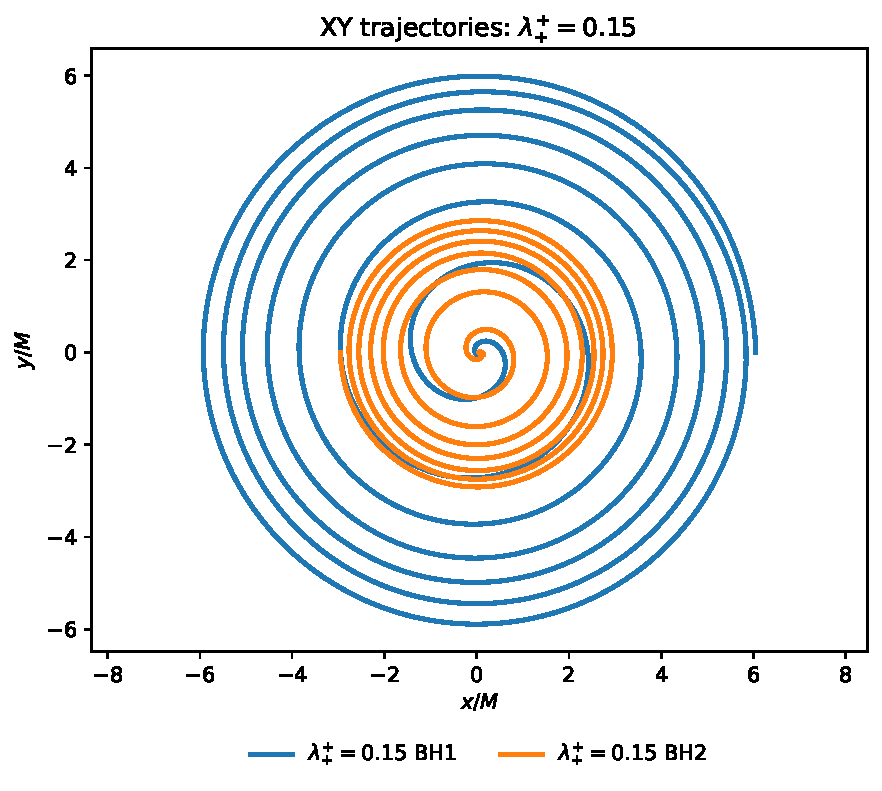
\includegraphics[height=0.22\textheight,keepaspectratio]{Figures/Chapter_2/Q2_SPIN_04_high_charge_Q0p15_pp_xy_trajectory.pdf}%
}

\caption{Orbital dynamics for the $q=1$ and $q=2$ configurations. For each mass ratio, the left panel shows the coordinate separation as a function of time, while the right panel shows representative coordinate trajectories in the orbital plane. The charge configuration affects both the inspiral time and the orbital phasing by modifying the effective interaction between the black holes. The trajectories are approximately quasicircular until the final plunge, which begins once the separation drops below roughly $6M$. Here $\lambda$ denotes the magnitude of the charge-to-mass ratio, $|Q|/M$, assigned to each charged black hole; neutral black holes have $\lambda=0$. The superscript and subscript indicate the charge configuration, with the larger black hole assigned the positive charge in unequal-mass cases. Thus, $\lambda^{+}_{+}$ denotes two positively charged black holes, $\lambda^{+}_{-}$ denotes oppositely charged black holes, and $\lambda^{+}_{0}$ denotes one positively charged and one neutral black hole. The $\lambda=0$ case is the GR reference waveform. In the trajectory plots, orange and blue denote the paths of the heavier and lighter black holes, respectively, with the initial data chosen so that the center of mass is at the origin.}
\label{fig:orbital_dynamics_q1_q2}

\end{figure}
\FloatBarrier
\begin{figure}[p]
\centering


\subfloat[$q=4$: black hole separation.\label{fig:bh_separation_q4}]{%
    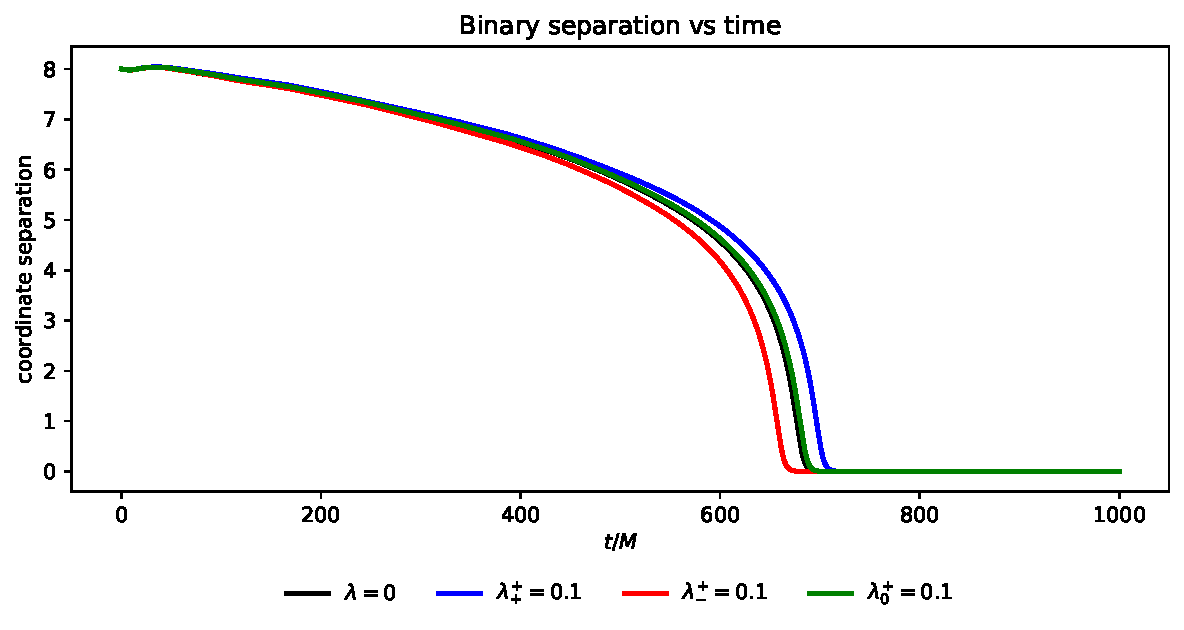
\includegraphics[height=0.22\textheight,keepaspectratio]{Figures/Chapter_2/Q4_spin04_high_charge_separation_comparison.pdf}%
}
\hfill
\subfloat[$q=4$: orbital trajectories.\label{fig:bh_xy_q4}]{%
    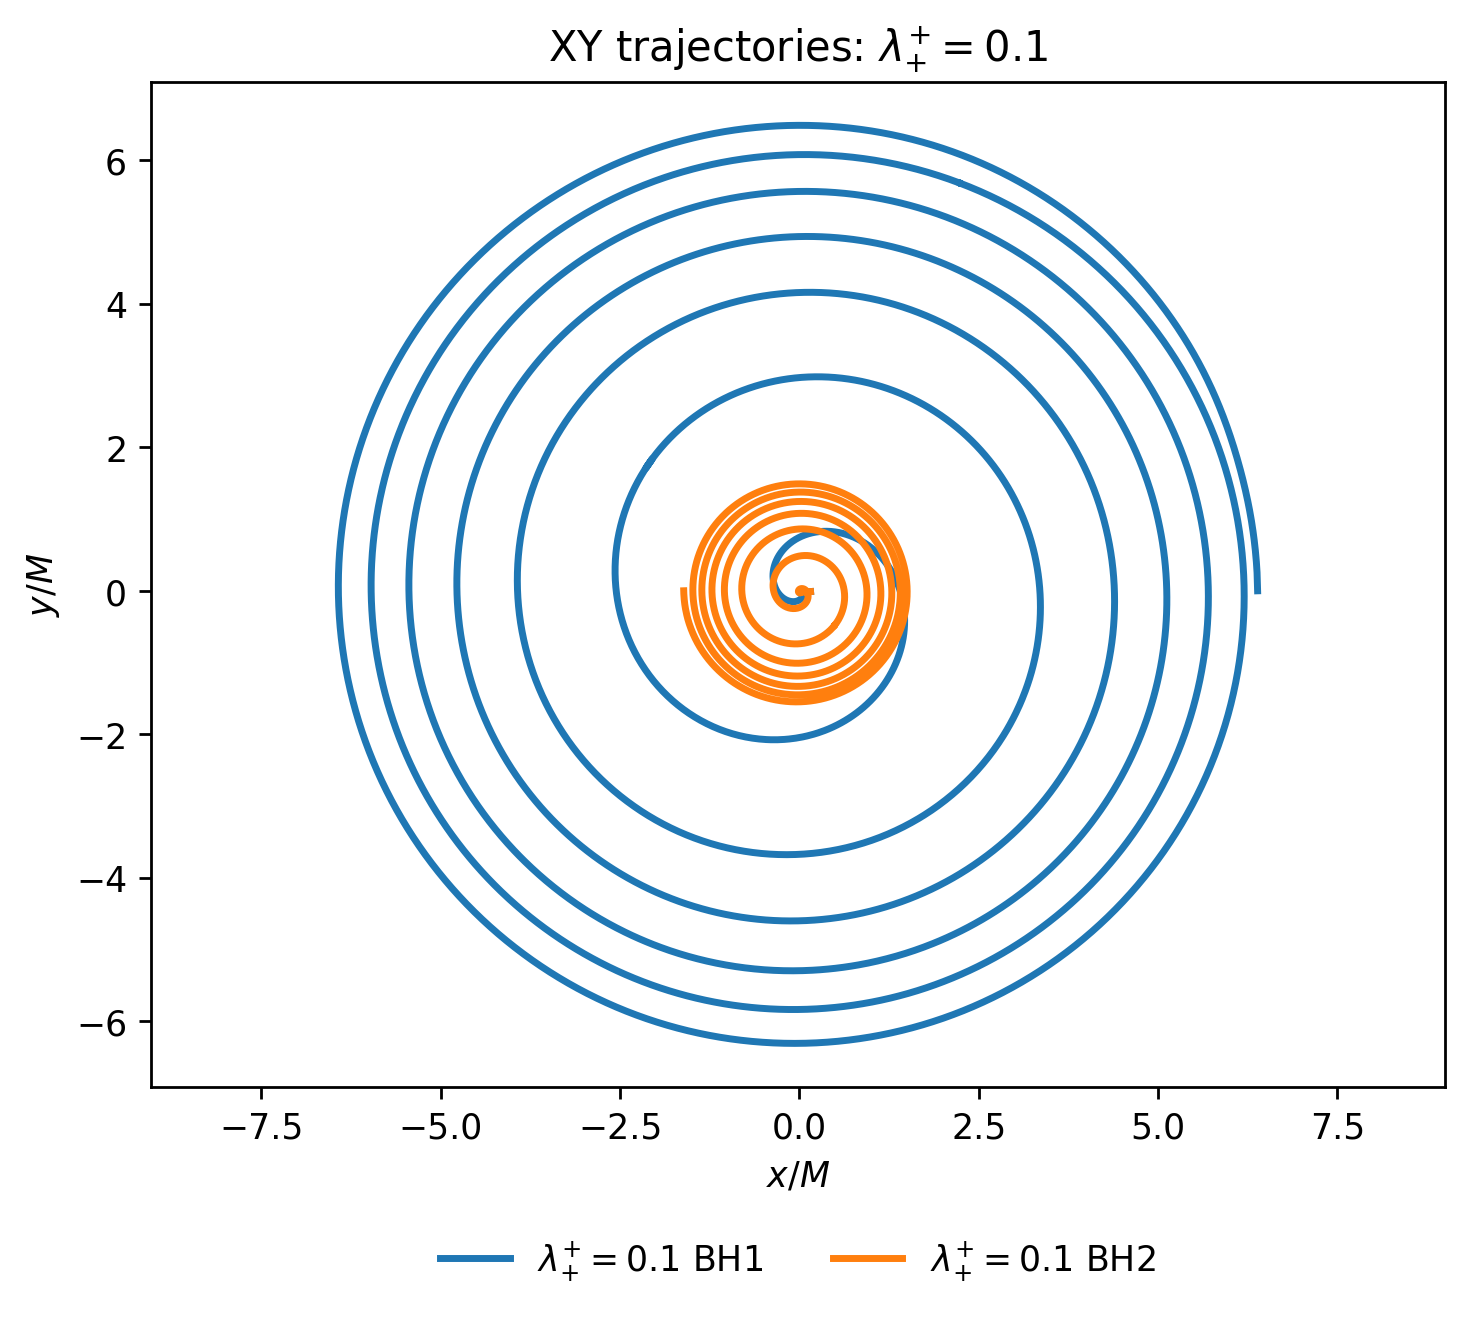
\includegraphics[height=0.22\textheight,keepaspectratio]{Figures/Chapter_2/Q4_spin04_high_charge_Q0p1_pp_xy_trajectory.png}%
}

\vspace{1.0em}

\subfloat[$q=8$: black hole separation.\label{fig:bh_separation_q8}]{%
    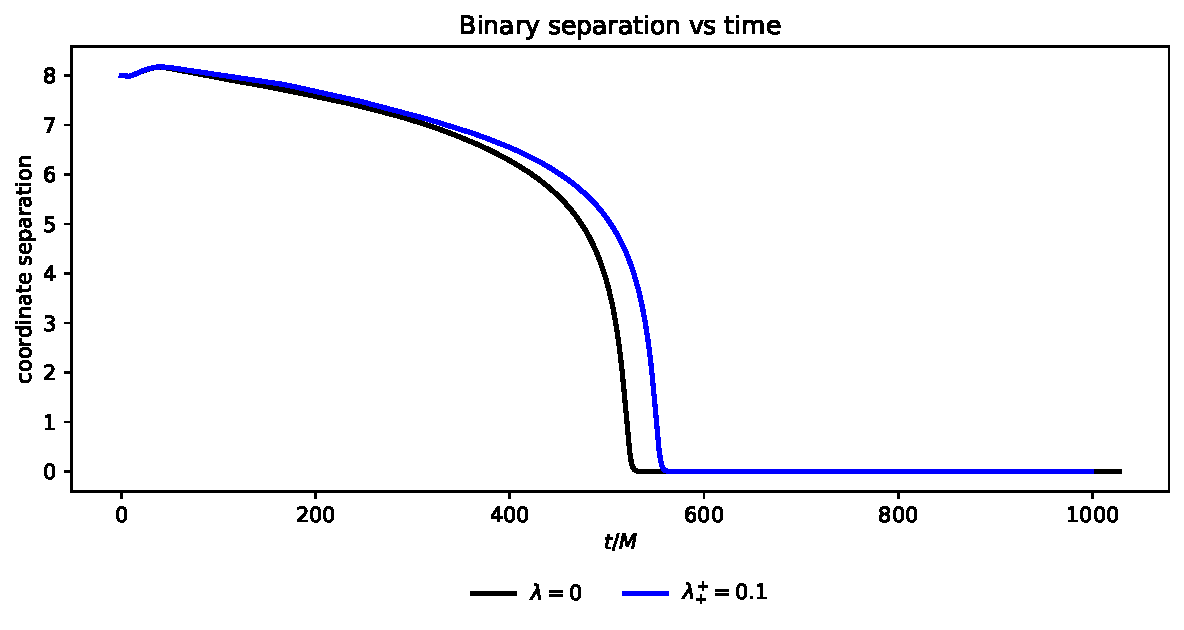
\includegraphics[height=0.22\textheight,keepaspectratio]{Figures/Chapter_2/Q8_SPIN_04_high_charge_separation_comparison.pdf}%
}
\hfill
\subfloat[$q=8$: orbital trajectories.\label{fig:bh_xy_q8}]{%
    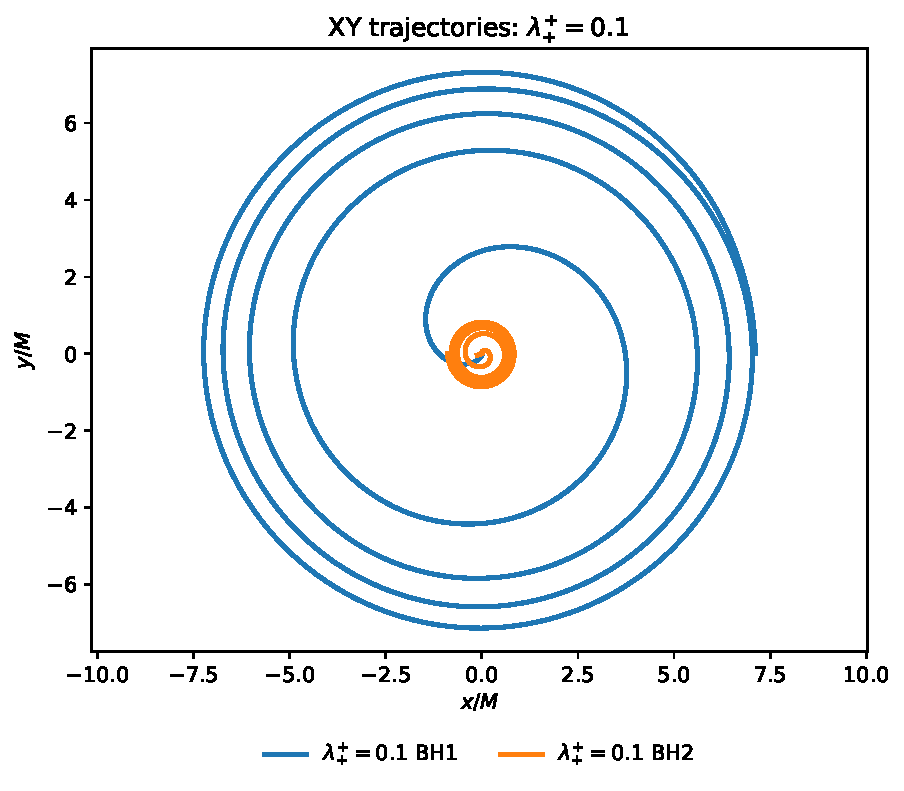
\includegraphics[height=0.22\textheight,keepaspectratio]{Figures/Chapter_2/Q8_SPIN_04_high_charge_Q0p1_pp_xy_trajectory.pdf}%
}

\caption{Orbital dynamics for the $q=4$ and $q=8$ configurations. For each mass ratio, the left panel shows the coordinate separation as a function of time, while the right panel shows representative coordinate trajectories in the orbital plane. The charge configuration affects both the inspiral time and the orbital phasing by modifying the effective interaction between the black holes. The trajectories are approximately quasicircular until the final plunge, which begins once the separation drops below roughly $6M$. Here $\lambda$ denotes the magnitude of the charge-to-mass ratio, $|Q|/M$, assigned to each charged black hole; neutral black holes have $\lambda=0$. The superscript and subscript indicate the charge configuration, with the larger black hole assigned the positive charge. Thus, $\lambda^{+}_{+}$ denotes two positively charged black holes, $\lambda^{+}_{-}$ denotes oppositely charged black holes, and $\lambda^{+}_{0}$ denotes one positively charged and one neutral black hole. The $\lambda=0$ case is the GR reference waveform. In the trajectory plots, orange and blue denote the paths of the heavier and lighter black holes, respectively, with the initial data chosen so that the center of mass is near the origin.}
\label{fig:orbital_dynamics_q4_q8}
\end{figure}
\FloatBarrier
We estimate the orbital eccentricity using an estimator based on the orbital frequency~\cite{RamosBuades2019_EccRed},
\begin{equation}
\varepsilon_{\Omega}(t)
=
\frac{1}{2}
\left[
\frac{\Omega(t)-\Omega_{e=0}(t)}
{\Omega_{e=0}(t)}
\right],
\label{eq:eccentricity_omega_estimator}
\end{equation}
where $\Omega(t)$ is the measured orbital frequency and $\Omega_{e=0}(t)$ denotes the corresponding non-eccentric orbital frequency.

We use an orbital-frequency-based estimator rather than one based directly on the coordinate separation, since separation-based measures can be strongly affected by gauge dynamics, while frequency-based eccentricity estimators are commonly used in eccentricity-reduction procedures \cite{Buonanno2011ReducingEccentricity,Lousto2013OuterLimits}. Although it is still not fully gauge invariant. We track the coordinate positions of each black hole during the inspiral, compute the coordinate separation, and then compute the orbital frequency. The orbital-frequency data are then fit using \verb|NonlinearModelFit| in \verb|Mathematica| with a post-Newtonian-inspired fitting model~\cite{RamosBuades2019_EccRed}.

When fitting the orbital-frequency data, it is useful to include as many orbits as possible in order to reduce the uncertainty in the eccentricity estimate. However, the early part of each simulation contains gauge-settling effects that are not associated with the physical orbital eccentricity, while the late part of the simulation is affected by the onset of plunge. We therefore exclude the first $\sim 200M$ of the simulation and choose the end of the fitting window before the rapid late-inspiral growth of the orbital frequency becomes dominant. In practice, this typically corresponds to ending the fit when the coordinate separation is of order $6M$. The need to have very small eccentricities is balanced by the cost of running runs with higher seperation that need more time to merge.

The measured orbital eccentricities for the catalog runs are shown in Table~\ref{tab:eccentricity_catalog}. The quoted eccentricities are extrapolated from the fit to $t=0M$. The initial coordinate separations are $r=10M$, $r=9M$, and $r=8M$ for the $q=1$, $q=2$, and $q=4$ or $q=8$ configurations, respectively. Most of the lower-spin and lower-charge configurations have eccentricities of order $10^{-3}$, while the largest eccentricities occur in the high-spin and high-charge equal-mass cases.

Figure~\ref{fig:bh_eccentricity} shows an example of the orbital-frequency eccentricity fit for one catalog run. This case has $q=1$, $\chi=0.4$, $\lambda=0.3$, and charge configuration $++$. The fit uses approximately four orbits, with $t_{\mathrm{min}}=200M$ and $t_{\mathrm{max}}=1300M$. The measured eccentricity extrapolated to $t=0M$ is $\varepsilon_\Omega=(14.44\pm0.33)\times10^{-3}$. This comparatively large eccentricity is consistent with the fact that this is a high-charge, like-signed configuration, for which the reduced effective attraction makes the initial momentum prescription less accurate.

In principle, lower eccentricities could be obtained through an iterative eccentricity-reduction procedure, in which the initial momenta are corrected after an initial eccentricity measurement and the simulation is repeated. We do not perform iterative eccentricity reduction for this exploratory catalog. Standard post-Newtonian eccentricity-reduction methods may also need modification in the EMDA case, since the electromagnetic, dilaton, and axion fields can affect the orbital dynamics. Developing eccentricity-reduction procedures that incorporate these effects is left for future work.

\begin{figure}[htbp]
\centering
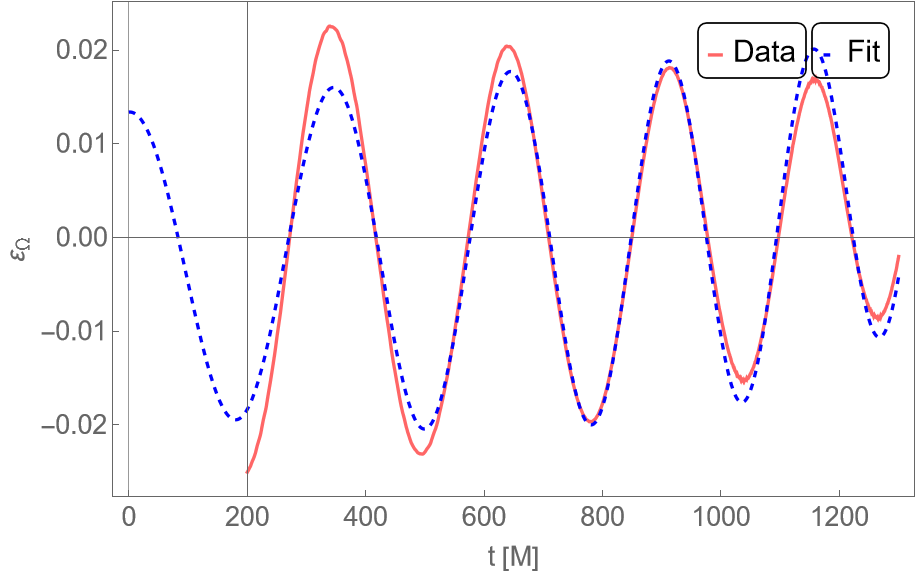
\includegraphics[width=0.48\textwidth]{Figures/Chapter_2/EMDA_eccentricity.png}
\caption{Measured orbital-frequency eccentricity and fitted eccentricity model for a binary black hole inspiral with $q=1$, $\chi=0.4$, $\lambda=0.3$, and charge configuration $++$. The fit is performed from $t_{\mathrm{min}}=200M$ to $t_{\mathrm{max}}=1300M$, excluding early gauge-settling effects and ending before the onset of plunge. The measured eccentricity extrapolated to $t=0M$ is $\varepsilon_\Omega=(14.44\pm0.33)\times10^{-3}$.}
\label{fig:bh_eccentricity}
\end{figure}

% \subsection{Simulation Setup}

\subsection{Waveform mismatch and distinguishability}
\label{sec:waveform_mismatch}

Following Refs.~\cite{Damour1998_ImprovedFilters,Harry2011_TargetedCoherentSearch,Abbott2017_WaveformSystematicsGW150914,Bozzola2021}, we use waveform overlaps and mismatches to quantify differences between the simulated gravitational wave signals.

A direct comparison between charged EMDA and neutral GR waveforms does not, by itself, isolate the contribution of the dilaton and axion fields. Part of the measured difference may arise from the electromagnetic charge and the associated change in the orbital dynamics, rather than from the additional EMDA fields alone. A more complete study would compare EMDA waveforms not only with neutral GR waveforms, but also with charged Einstein--Maxwell evolutions having the same charge configurations. Such a comparison is beyond the scope of the present work. Our goal here is instead to quantify the fixed parameter waveform differences between charged EMDA binaries and their neutral GR counterparts.

To quantify the difference between two gravitational wave signals, we compute the mismatch
\begin{equation}
\mathcal{M}(h_1,h_2)
=
1-\lbrack \max_{\Delta t,\Delta\varphi}\mathcal{O}(h_1,h_2)\rbrack,
\label{eq:mismatch_def}
\end{equation}
where the maximum is taken over relative time shifts $\Delta t$ and polarization-angle shifts $\Delta\varphi$. The overlap $\mathcal{O}$ is defined by
\begin{equation}
\mathcal{O}(h_1,h_2)
=
\frac{(h_1,h_2)}
{\sqrt{(h_1,h_1)(h_2,h_2)}} ,
\label{eq:overlap_def}
\end{equation}
where $(h_1,h_2)$ denotes the detector-noise-weighted inner product between the two waveforms. In practice, this inner product is evaluated over the finite frequency range used in the analysis, with the same preprocessing choices applied to each waveform pair.

The comparison performed here does not maximize over intrinsic binary parameters such as the masses, spins, eccentricity, or charge. These degeneracies could partially obscure the waveform differences found in a fixed parameter comparison and would likely make charge-induced deviations more difficult to identify in a full parameter-estimation study. The mismatch values reported below should therefore be interpreted as a measure of waveform separation at fixed intrinsic parameters, rather than as evidence for a unique observational signature of EMDA theory.

As a rough estimate of distinguishability, we associate a mismatch $\mathcal{M}$ with the critical signal-to-noise ratio
\begin{equation}
\rho_{\rm crit}
\simeq
\frac{1}{\sqrt{2\mathcal{M}}}.
\label{eq:rho_crit}
\end{equation}
This estimate gives the signal-to-noise ratio at which two waveforms with mismatch $\mathcal{M}$ would be expected to become distinguishable in an idealized fixed parameter comparison. 

\section{Results}
\label{sec:results}

We compare charged EMDA waveforms with neutral GR reference waveforms for a representative set of binary black hole configurations. The purpose of this comparison is to determine how the waveform differences depend on charge magnitude, charge configuration, mass ratio, and spin. In each case, the charged EMDA waveform is compared against a neutral reference waveform with the same mass ratio and spin.

The simulation catalog considered in this chapter is summarized in Table~\ref{tab:simulation_catalog}. For each choice of mass ratio $q=m_1/m_2$, spin $\chi$, and charge magnitude $\lambda=|Q|/M$, we consider one neutral configuration, $Q_1=Q_2=0$, and several charged configurations. We label the charged cases by the signs of the two black hole charges. The cases $++$, $+-$, and $+0$ denote similar charges, oppositely signed charges, and a configuration with one charged and one neutral black hole, respectively. For unequal-mass binaries, the larger black hole is assigned the positive charge in the $+-$ and $+0$ cases.

Representative peak-aligned waveforms are shown in Fig.~\ref{fig:peak_aligned_hplus_all_mass_ratios}. The figure compares the strain component $r h_+$ for selected charged EMDA configurations against the corresponding neutral GR reference waveform. The waveforms are aligned at the peak amplitude in order to emphasize differences in the late inspiral, merger, and ringdown. Even after this alignment, the charged and neutral waveforms show visible phase and amplitude differences, indicating that charge and the additional EMDA fields can modify the binary dynamics prior to merger as well as the waveform near peak emission.

\begin{figure*}[t]
\centering

\subfloat[$q=1$.\label{fig:q1_peak_aligned_hplus}]{%
    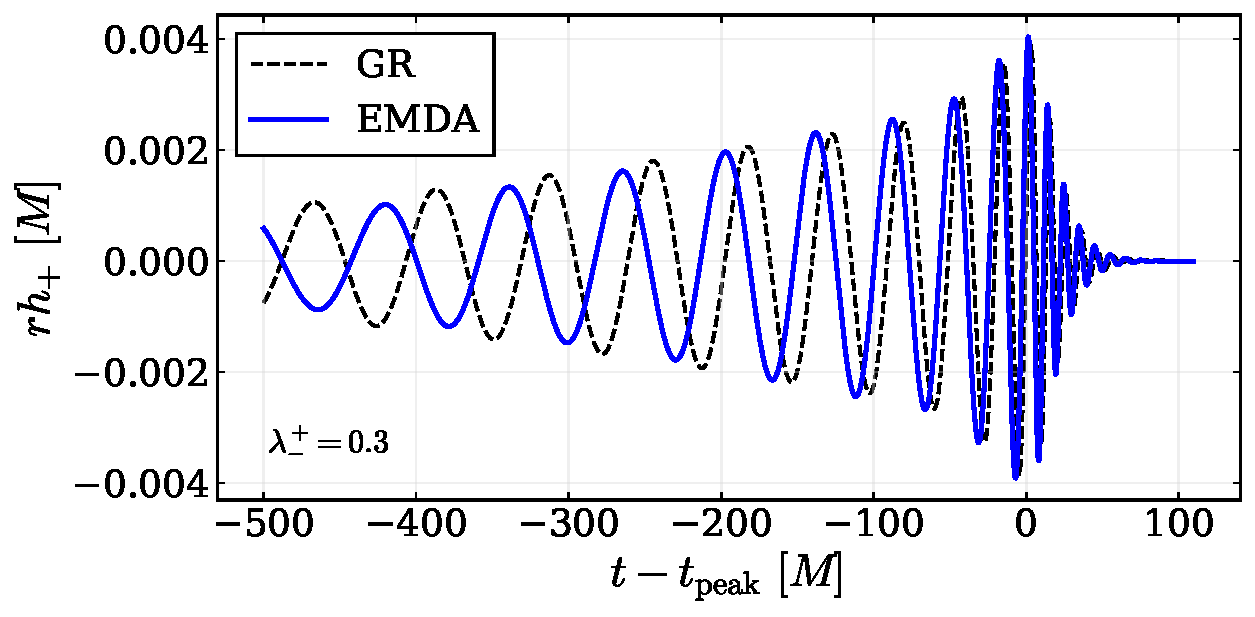
\includegraphics[width=0.48\textwidth]{Figures/Chapter_2/q1_Q0_vs_Q0p15_pn_peak_aligned_hplus_notitle.pdf}%
}
\hfill
\subfloat[$q=2$.\label{fig:q2_peak_aligned_hplus}]{%
    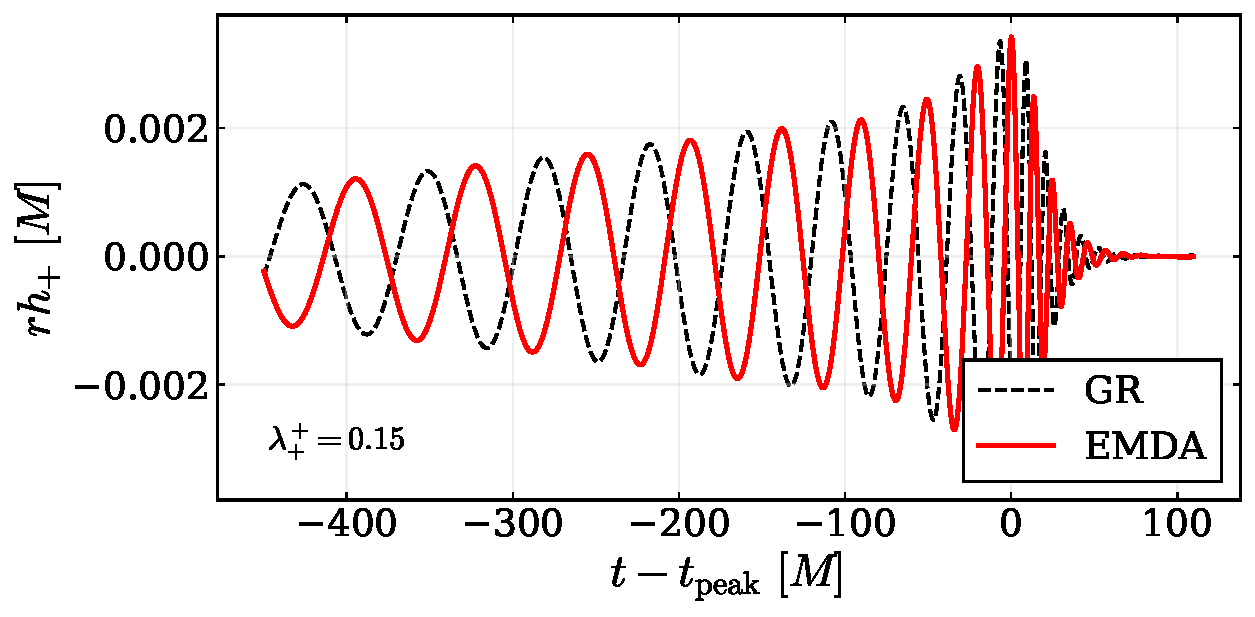
\includegraphics[width=0.48\textwidth]{Figures/Chapter_2/q2_Q0_vs_Q0p15_pp_peak_aligned_hplus_notitle.pdf}%
}

\vspace{0.5em}

\subfloat[$q=4$.\label{fig:q4_peak_aligned_hplus}]{%
    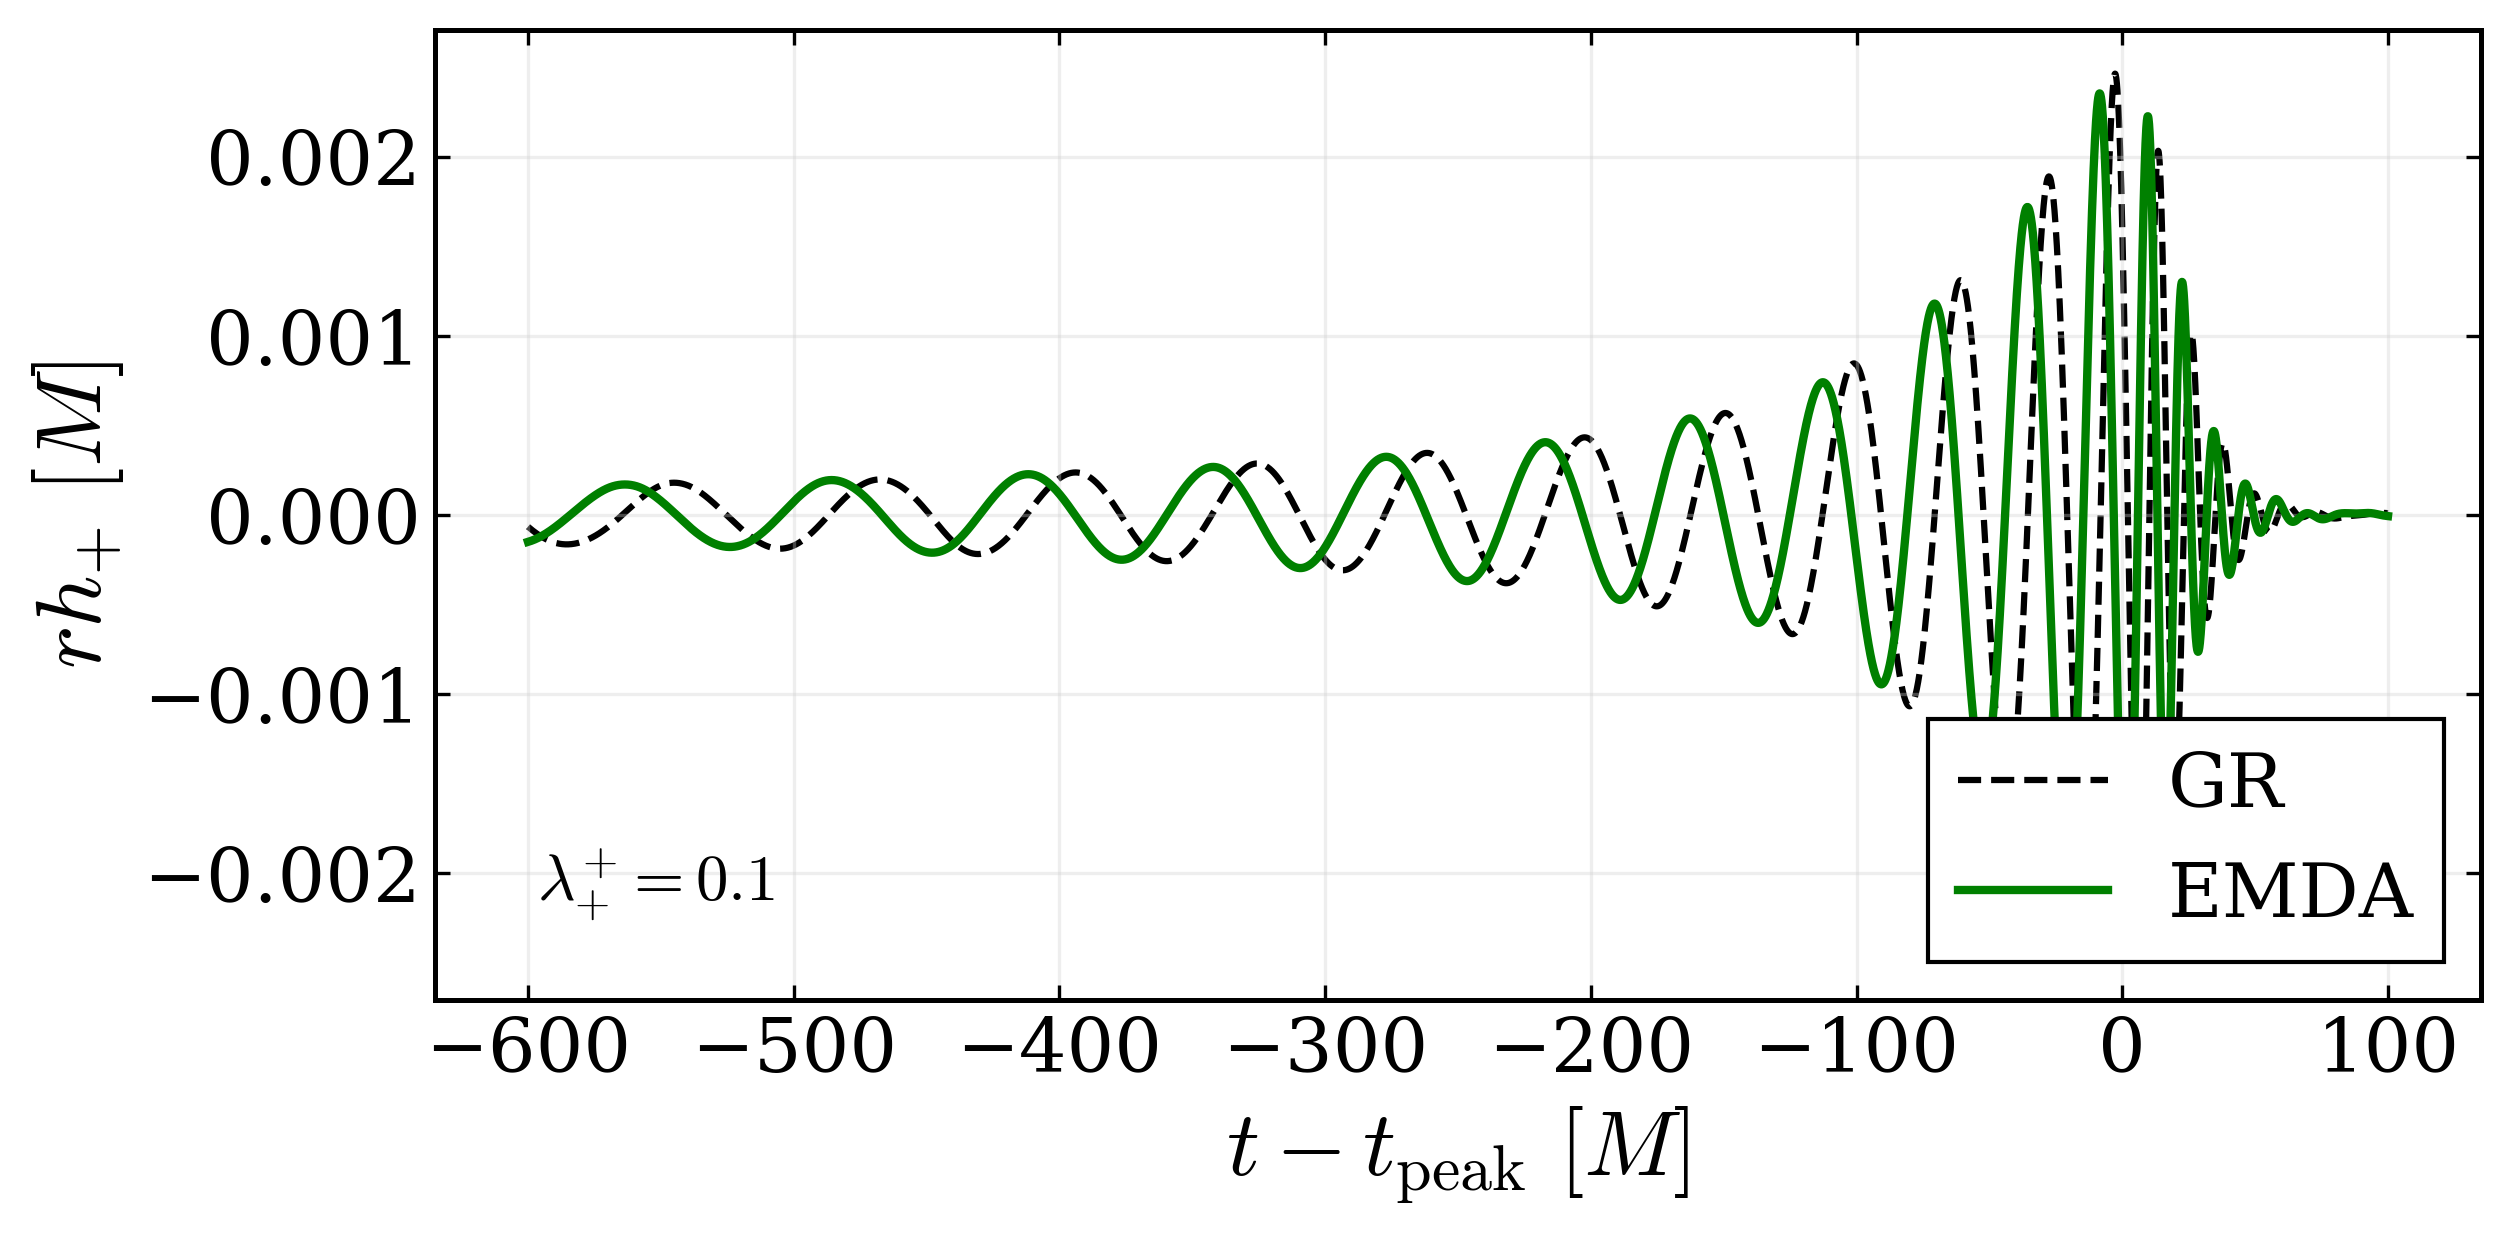
\includegraphics[width=0.48\textwidth]{Figures/Chapter_2/Q0_vs_Q0p1_pp_peak_aligned_hplus_notitle.png}%
}
\hfill
\subfloat[$q=8$.\label{fig:q8_peak_aligned_hplus}]{%
    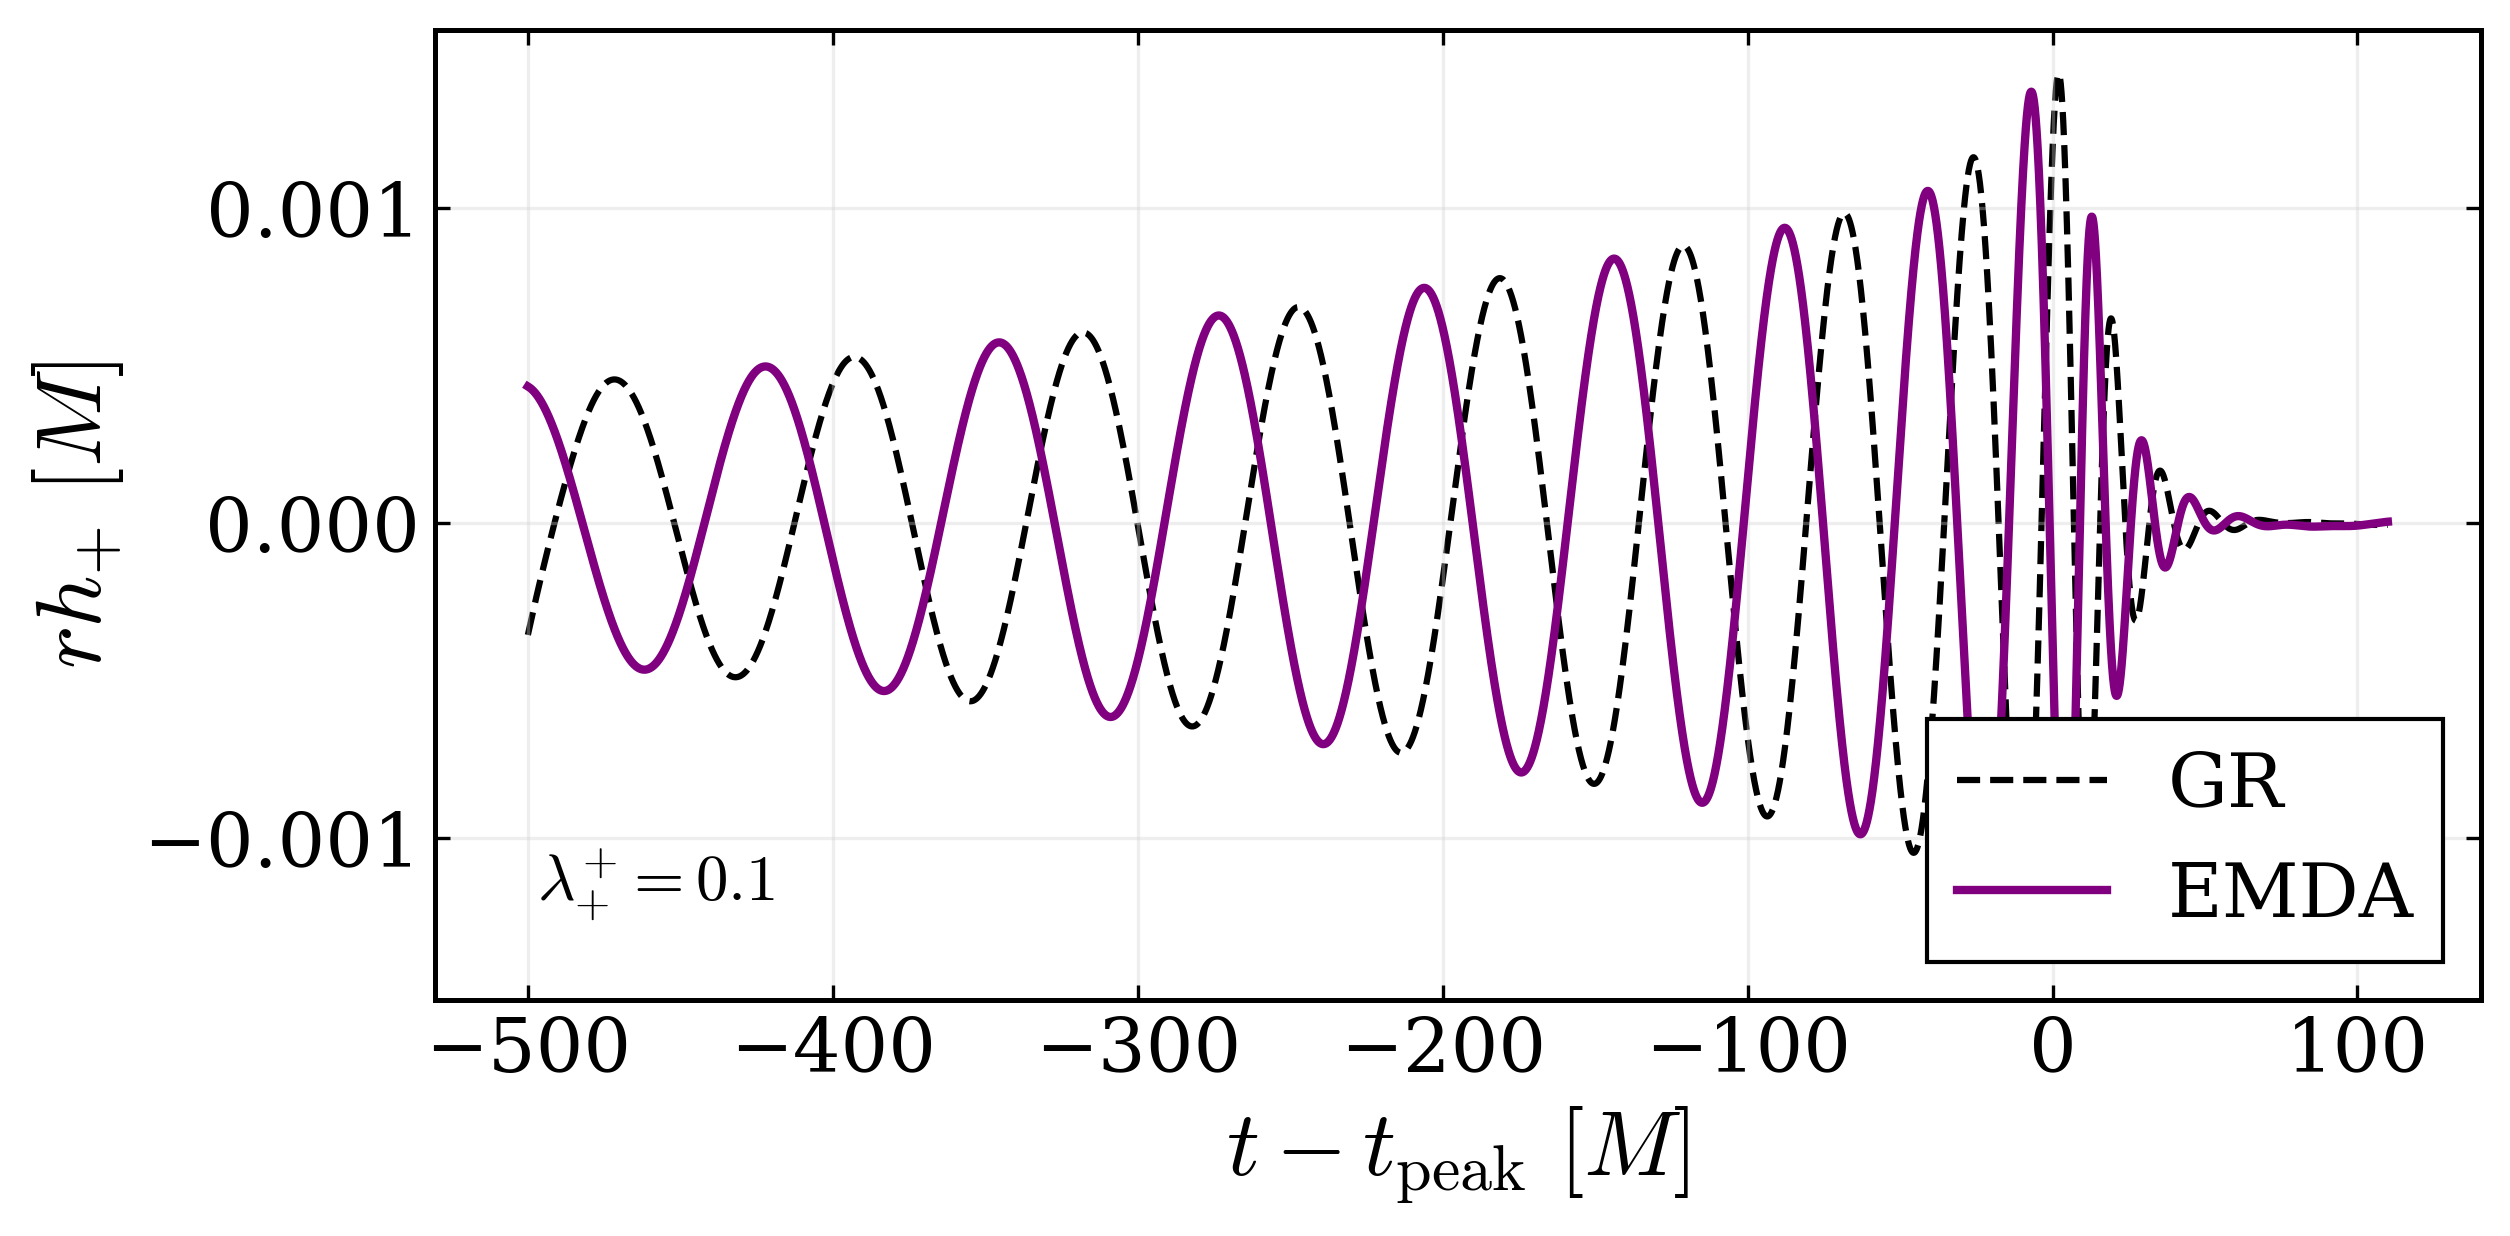
\includegraphics[width=0.48\textwidth]{Figures/Chapter_2/q8_Q0_vs_Q0p1_pp_peak_aligned_hplus_notitle.png}%
}

\caption{Peak-aligned comparisons of the gravitational wave strain component $r h_{+}$ for representative charged EMDA configurations against the corresponding neutral GR reference waveforms. In each panel, the time coordinate is shifted so that the waveform peak occurs at $t-t_{\mathrm{peak}}=0$. The remaining differences after peak alignment reflect changes in the accumulated phase, merger time, and waveform morphology.}
\label{fig:peak_aligned_hplus_all_mass_ratios}

\end{figure*}

The full set of waveform mismatches is computed using the numerical-relativity analysis toolkit \texttt{kuibit}~\cite{kuibit}. kuibit is a numerical relativity library with functions to process gravitational waves.  The results are given in Table~\ref{tab:waveform_mismatches_combined}. The mismatch values generally increase with charge magnitude, although the trend is not monotonic across all spin and charge configurations. For example, in the $q=1$, $\chi=0.4$, $++$ sequence, the mismatch increases from $2.60\times10^{-4}$ for $\lambda=0.1$ to $5.28\times10^{-3}$ for $\lambda=0.3$. Similar growth with charge is seen in several other equal-mass configurations.

The charge configuration also plays an important role. The $++$, $+-$, and $+0$ cases do not produce equivalent waveform differences, even at the same charge magnitude. In many cases, the singly charged $+0$ configurations remain closer to the neutral reference waveform than the corresponding two-charged configurations. This is consistent with the expectation that the strength and symmetry of the charge distribution influence both the orbital dynamics and the matter-field content of the spacetime. Oppositely signed charges can also produce comparatively large mismatches, since the electromagnetic interaction increases the effective attraction and changes the inspiral rate.

The $\chi=0.8$ equal-mass configurations are somewhat anomalous compared with the lower-spin cases. While the mismatch generally grows with charge for the lower-spin sequences, the $\chi=0.8$ cases show larger and less monotonic variations across the different charge configurations. These runs also have noticeably larger eccentricities, especially at the highest charge magnitudes, suggesting that the approximate charged initial-data prescription is being pushed beyond the regime where it gives uniformly low-eccentricity inspirals. We therefore include these cases as useful indicators of where large waveform differences can occur, but we do not interpret their detailed mismatch hierarchy as a clean physical trend.

The high-spin configurations nevertheless show the largest waveform separations in the catalog. For the $q=1$, $\chi=0.8$ cases, some mismatches reach the $10^{-2}$--$10^{-1}$ level. These large values indicate that the charged and neutral waveforms are substantially separated at fixed intrinsic parameters. However, because these cases are also more sensitive to eccentricity and initial-data systematics, they should not be interpreted as isolated signatures of the dilaton or axion fields.

The critical signal-to-noise ratio estimate associated with the mismatch values spans approximately $\rho_{\rm crit}\sim2.3$ to over 500 across the catalog. These values should be understood as fixed parameter distinguishability estimates: they indicate the signal-to-noise ratio at which the charged EMDA waveform and the corresponding neutral GR waveform would become distinguishable if the intrinsic binary parameters were held fixed. In a full parameter-estimation study, changes in the masses, spins, eccentricity, or other parameters could partially obscure these differences. The mismatch values therefore quantify waveform separation within this catalog, rather than providing direct observational bounds on EMDA theory.

These results demonstrate that our EMDA evolution framework can produce a range of charged binary black hole simulations with relatively low eccentricity. For most of the catalog, the observed waveform trends are consistent with physical expectations: increasing the charge magnitude tends to increase the waveform mismatch, and different charge configurations produce distinct inspiral and merger behavior. Nevertheless, the highest-spin configurations require additional caution. These cases show larger residual eccentricities and noisier waveforms than the lower-spin runs, suggesting that the approximate charged initial-data prescription and the chosen grid resolution may be less reliable in this region of parameter space. Future work should revisit these cases with improved eccentricity reduction and higher-resolution simulations to determine whether the large waveform differences remain after these numerical effects are better controlled.
\section{Conclusion}
\label{sec:conclusion}

In this chapter, we presented an exploratory waveform catalog for charged binary black hole simulations in Einstein--Maxwell--dilaton--axion (EMDA) theory. We compared the resulting charged EMDA waveforms with neutral general-relativistic reference waveforms having the same mass ratio and spin. Across much of the catalog, the waveform differences increase with the charge magnitude, indicating that charge and the additional EMDA fields can produce appreciable changes in the gravitational wave signal. The trend is clearest in the lower-spin configurations, while the highest-spin cases show larger and less monotonic differences that are likely more sensitive to eccentricity and the approximate charged initial-data prescription.

Using the mismatch as a rough fixed parameter distinguishability estimate, the largest waveform separations in the catalog correspond to critical signal-to-noise ratios, with the smallest values approximately $\rho_{\rm crit}\sim2.3$. These values indicate that the largest charged EMDA deviations from the corresponding neutral GR waveforms are substantial at fixed intrinsic parameters. However, they should not be interpreted as direct observational thresholds or constraints on EMDA theory. A full parameter-estimation study would be required to determine whether these differences could be mimicked by changes in the masses, spins, eccentricity, total mass scale, or other binary parameters.

The waveform differences found here should also be interpreted with care because the comparison is made against neutral GR rather than against charged Einstein--Maxwell binaries. As a result, the reported mismatches include the combined effect of electric charge, modified orbital dynamics, and the additional dilaton and axion fields. They cannot be attributed uniquely to the dilaton or axion fields alone. A more complete comparison would include corresponding Einstein--Maxwell simulations with the same charge configurations, allowing the purely electromagnetic contribution to be separated from the additional EMDA-field effects.

These results demonstrate that EMDA theory provides a useful numerical-relativity testbed for studying charged beyond-GR effects in binary black hole mergers. Even within this exploratory catalog, charged EMDA binaries can produce waveform differences that are large enough to motivate further study. Natural next steps include larger parameter surveys, improved charged initial data, iterative eccentricity reduction, longer inspirals, and convergence studies of the waveform mismatches. It would be especially useful to extend the high-mass-ratio portion of the catalog by performing additional $q=8$ simulations with the full set of charge configurations, higher spins, and larger charge magnitudes. Direct comparisons among neutral GR, charged Einstein--Maxwell, and charged EMDA binaries would also help separate ordinary electromagnetic effects from waveform changes associated specifically with the dilaton and axion fields.
\section{Simulation Catalog}
\label{sec:simulation_catalog}

The simulations used in this chapter are summarized in Table~\ref{tab:simulation_catalog}. The catalog samples several mass ratios, spin values, charge magnitudes, and charge configurations. For each mass ratio and spin, we include a neutral reference simulation and compare the charged EMDA evolutions against that corresponding neutral case.
\FloatBarrier
\begin{table*}[htbp]
\centering
\caption{EMDA binary black hole simulation catalog. Here $q=m_1/m_2$ denotes the mass ratio, $\chi$ denotes the dimensionless spin parameter, and $\lambda_i=Q_i/M_i$ denotes the charge-to-mass ratio of black hole $i$. The neutral case corresponds to $Q_1=Q_2=0$. For charged configurations, the magnitude of the nonzero charge-to-mass ratios is denoted by $\lambda$, with the sign structure indicated by the charge configuration. The configurations $++$, $+-$, and $+0$ denote like-signed charges, oppositely signed charges, and cases in which only one black hole is charged, respectively. Because the neutral configuration is independent of $\lambda$, it is listed only once for each mass ratio and spin.}
\label{tab:simulation_catalog}
\begin{tabular}{ccccccc}
\toprule
Mass Ratio $q$ & Spin $\chi$ & Charge Magnitude $\lambda$ & Neutral & $++$ & $+-$ & $+0$ \\
\midrule
1 & 0.0 & 0.1 & $\checkmark$ & $\checkmark$ & $\checkmark$ & $\checkmark$ \\
1 & 0.0 & 0.2 & -- & $\checkmark$ & $\checkmark$ & $\checkmark$ \\
1 & 0.0 & 0.3 & -- & $\checkmark$ & $\checkmark$ & $\checkmark$ \\
\midrule
1 & 0.4 & 0.1 & $\checkmark$ & $\checkmark$ & $\checkmark$ & $\checkmark$ \\
1 & 0.4 & 0.2 & -- & $\checkmark$ & $\checkmark$ & $\checkmark$ \\
1 & 0.4 & 0.3 & -- & $\checkmark$ & $\checkmark$ & $\checkmark$ \\
\midrule
1 & 0.8 & 0.1 & $\checkmark$ & $\checkmark$ & $\checkmark$ & $\checkmark$ \\
1 & 0.8 & 0.2 & -- & $\checkmark$ & $\checkmark$ & $\checkmark$ \\
1 & 0.8 & 0.3 & -- & $\checkmark$ & $\checkmark$ & $\checkmark$ \\
\midrule
2 & 0.0 & 0.05 & $\checkmark$ & $\checkmark$ & $\checkmark$ & $\checkmark$ \\
2 & 0.0 & 0.15 & -- & $\checkmark$ & $\checkmark$ & $\checkmark$ \\
\midrule
2 & 0.4 & 0.05 & $\checkmark$ & $\checkmark$ & $\checkmark$ & $\checkmark$ \\
2 & 0.4 & 0.15 & -- & $\checkmark$ & $\checkmark$ & $\checkmark$ \\
\midrule
4 & 0.4 & 0.05 & $\checkmark$ & $\checkmark$ & $\checkmark$ & $\checkmark$ \\
4 & 0.4 & 0.10 & -- & $\checkmark$ & $\checkmark$ & $\checkmark$ \\
\midrule
8 & -0.2 & 0.10 & $\checkmark$ & $\checkmark$ & -- & -- \\
\bottomrule
\end{tabular}
\end{table*}
The simulations used in this chapter are summarized in Table~\ref{tab:simulation_catalog}. The catalog samples several mass ratios, spin values, charge magnitudes, and charge configurations. For each mass ratio and spin, we include a neutral reference simulation and compare the charged EMDA evolutions against that corresponding neutral case. For the $q=8$ simulations, we choose a negative spin value, $\chi=-0.2$, corresponding to spin anti-aligned with the orbital angular momentum. This choice reduces the inspiral time relative to an aligned-spin configuration, making the high-mass-ratio simulations less computationally expensive.
\FloatBarrier
\begin{table*}[t]
\centering
\caption{Mismatch of charged EMDA binary black hole waveforms relative to the corresponding neutral reference waveform \texttt{Q0}. Here $q=m_1/m_2$, $\chi$ is the dimensionless spin parameter, and $\lambda_i=Q_i/M_i$. The column $|\lambda_i|$ gives the magnitude of the nonzero charge-to-mass ratio used in each charged configuration. The columns $++$, $+-$, and $+0$ denote like-signed charges, oppositely signed charges, and configurations in which only one black hole is charged, respectively. The mismatch is computed from the $(\ell,m)=(2,2)$ gravitational waveform using the numerical-relativity analysis package \texttt{kuibit}, after optimizing over relative time and polarization shifts. The values in parentheses give the approximate fixed parameter critical signal-to-noise ratio, $\rho_{\rm crit}\simeq 1/\sqrt{2\mathcal{M}}$. These values should be interpreted as rough waveform-separation estimates rather than full observational detection thresholds.}
\label{tab:waveform_mismatches_combined}
\scriptsize
\setlength{\tabcolsep}{4pt}
\renewcommand{\arraystretch}{1.08}
\resizebox{\textwidth}{!}{%
\begin{tabular}{cccccc}
\toprule
Mass Ratio $q$ & Spin $\chi$ & Charge Magnitude $|\lambda_i|$
& $++$ & $+-$ & $+0$ \\
\midrule
1 & 0.0 & 0.10 & $3.53\times 10^{-4};(37.6)$ & $2.74\times 10^{-4};(42.8)$ & $1.55\times 10^{-4};(56.8)$ \\
1 & 0.0 & 0.20 & $6.71\times 10^{-4};(27.3)$ & $1.45\times 10^{-3};(18.5)$ & $6.91\times 10^{-4};(26.9)$ \\
1 & 0.0 & 0.30 & $1.94\times 10^{-3};(16.0)$ & $5.32\times 10^{-3};(9.7)$ & $7.54\times 10^{-4};(25.8)$ \\
\midrule
1 & 0.4 & 0.10 & $2.60\times 10^{-4};(43.9)$ & $2.87\times 10^{-4};(41.8)$ & $4.08\times 10^{-4};(35.0)$ \\
1 & 0.4 & 0.20 & $7.10\times 10^{-4};(26.5)$ & $7.40\times 10^{-3};(8.2)$ & $7.42\times 10^{-4};(26.0)$ \\
1 & 0.4 & 0.30 & $5.28\times 10^{-3};(9.7)$ & $2.90\times 10^{-2};(4.1)$ & $1.04\times 10^{-3};(21.9)$ \\
\midrule
1 & 0.8 & 0.10 & $2.77\times 10^{-4};(42.5)$ & $9.44\times 10^{-4};(23.0)$ & $1.03\times 10^{-3};(22.0)$ \\
1 & 0.8 & 0.20 & $4.66\times 10^{-2};(3.3)$ & $9.30\times 10^{-2};(2.3)$ & $1.67\times 10^{-2};(5.5)$ \\
1 & 0.8 & 0.30 & $6.19\times 10^{-2};(2.8)$ & $2.53\times 10^{-2};(4.4)$ & $7.99\times 10^{-3};(7.9)$ \\
\midrule
2 & 0.0 & 0.05 & $1.58\times 10^{-3};(17.8)$ & $1.34\times 10^{-3};(19.3)$ & $2.56\times 10^{-5};(139.7)$ \\
2 & 0.0 & 0.15 & $1.83\times 10^{-3};(16.5)$ & $3.21\times 10^{-3};(12.5)$ & $7.47\times 10^{-4};(25.9)$ \\
\midrule
2 & 0.4 & 0.05 & $7.27\times 10^{-5};(82.9)$ & $1.33\times 10^{-4};(61.3)$ & $1.73\times 10^{-6};(537.4)$ \\
2 & 0.4 & 0.15 & $6.17\times 10^{-4};(28.5)$ & $2.34\times 10^{-4};(46.2)$ & $7.58\times 10^{-5};(81.2)$ \\
\midrule
4 & 0.4 & 0.05 & $5.10\times 10^{-5};(99.0)$ & $7.34\times 10^{-5};(82.5)$ & $7.17\times 10^{-5};(83.5)$ \\
4 & 0.4 & 0.10 & $3.17\times 10^{-4};(39.7)$ & $1.82\times 10^{-4};(52.5)$ & $8.80\times 10^{-5};(75.4)$ \\
\midrule
8 & -0.2 & 0.10 & $1.14\times 10^{-3};(21.0)$ & \text{--} & \text{--} \\
\bottomrule
\end{tabular}%
}
\end{table*}
Table~\ref{tab:waveform_mismatches_combined} summarizes the fixed parameter waveform mismatches between the charged EMDA simulations and the corresponding neutral reference waveforms. Across much of the catalog, the mismatch increases with charge magnitude, although the trend is not strictly monotonic for every spin and charge configuration. The clearest growth occurs in the equal-mass lower-spin cases. For example, for $q=1$ and $\chi=0.4$, the $++$ mismatch grows from $2.60\times10^{-4}$ at $\lambda=0.1$ to $5.28\times10^{-3}$ at $\lambda=0.3$, while the $+-$ mismatch grows even more strongly, reaching $2.90\times10^{-2}$. The charge configuration also has a significant effect: the $+0$ cases are often closer to the neutral reference waveform than the two-charged configurations, while the $+-$ cases can produce relatively large mismatches because the opposite charges increase the effective attraction and accelerate the inspiral. The largest mismatches occur in the high-spin $q=1$, $\chi=0.8$ cases, where some values reach the $10^{-2}$--$10^{-1}$ level; however, these cases should be interpreted with caution because they also have larger residual eccentricities and noisier waveforms. For the unequal-mass cases, especially $q=2$ and $q=4$, the mismatches are generally smaller, with many values below $10^{-3}$. Overall, the table shows that charge can produce measurable waveform differences at fixed mass ratio and spin, but that the size of the effect depends strongly on charge magnitude, charge configuration, and spin.
\section{Measured Eccentricities}
\label{sec:measured_eccentricities}

Table~\ref{tab:eccentricity_catalog} summarizes the measured orbital eccentricities for the EMDA waveform catalog. The values are obtained from the orbital-frequency eccentricity estimator described in Sec.~\ref{sec:eccentricity_control} and are reported as $(\varepsilon_\Omega \pm \delta\varepsilon_\Omega)\times10^3$.

\begin{table*}[htbp]
\centering
\caption{Measured orbital eccentricities for the EMDA waveform catalog. The entries are reported as $(\varepsilon_\Omega \pm \delta\varepsilon_\Omega)\times10^3$. Here $q=m_1/m_2$ denotes the mass ratio, $\chi$ denotes the dimensionless spin parameter, and $\lambda_i=Q_i/M_i$ denotes the charge-to-mass ratio of black hole $i$. The neutral case corresponds to $Q_1=Q_2=0$. For charged configurations, the magnitude of the nonzero charge-to-mass ratios is denoted by $\lambda$, with the sign structure indicated by the charge configuration. The configurations $++$, $+-$, and $+0$ denote like-signed charges, oppositely signed charges, and cases in which only one black hole is charged, respectively.}
\label{tab:eccentricity_catalog}
\begin{tabular}{ccccccc}
\toprule
Mass Ratio $q$ & Spin $\chi$ & Charge Magnitude $\lambda$ & Neutral & $++$ & $+-$ & $+0$ \\
\midrule
1 & 0.0 & 0.10 & $1.59 \pm 0.21$ & $2.57 \pm 0.17$ & $1.97 \pm 0.27$ & $2.54 \pm 0.23$ \\
1 & 0.0 & 0.20 & -- & $6.26 \pm 0.26$ & $3.52 \pm 0.35$ & $4.41 \pm 0.24$ \\
1 & 0.0 & 0.30 & -- & $14.99 \pm 0.40$ & $2.08 \pm 0.36$ & $5.28 \pm 0.45$ \\
\midrule
1 & 0.4 & 0.10 & $1.39 \pm 0.10$ & $1.80 \pm 0.11$ & $1.30 \pm 0.13$ & $1.26 \pm 0.11$ \\
1 & 0.4 & 0.20 & -- & $5.17 \pm 0.18$ & $1.04 \pm 0.22$ & $2.68 \pm 0.18$ \\
1 & 0.4 & 0.30 & -- & $14.44 \pm 0.33$ & $4.89 \pm 0.53$ & $4.19 \pm 0.19$ \\
\midrule
1 & 0.8 & 0.10 & $3.47 \pm 0.23$ & $3.23 \pm 0.18$ & $2.31 \pm 0.23$ & $2.31 \pm 0.21$ \\
1 & 0.8 & 0.20 & -- & $4.95 \pm 0.64$ & $5.44 \pm 0.71$ & $4.57 \pm 0.27$ \\
1 & 0.8 & 0.30 & -- & $44.75 \pm 0.70$ & $22.70 \pm 6.36$ & $13.03 \pm 2.02$ \\
\midrule
2 & 0.0 & 0.05 & $2.16 \pm 0.60$ & $1.98 \pm 0.22$ & $1.22 \pm 0.62$ & $1.62 \pm 0.31$ \\
2 & 0.0 & 0.15 & -- & $4.65 \pm 0.36$ & $2.18 \pm 0.33$ & $3.05 \pm 0.37$ \\
\midrule
2 & 0.4 & 0.05 & $1.68 \pm 0.11$ & $1.46 \pm 0.24$ & $1.78 \pm 0.14$ & $1.48 \pm 0.17$ \\
2 & 0.4 & 0.15 & -- & $5.19 \pm 0.15$ & $1.35 \pm 0.24$ & $2.09 \pm 0.18$ \\
\midrule
4 & 0.4 & 0.05 & $1.66 \pm 0.43$ & $1.44 \pm 0.32$ & $1.93 \pm 0.34$ & $1.49 \pm 0.50$ \\
4 & 0.4 & 0.10 & -- & $1.01 \pm 0.09$ & $0.81 \pm 0.21$ & $0.79 \pm 0.21$ \\
\midrule
8 & -0.2 & 0.10 & $4.88 \pm 61.91$ & $1.45 \pm 5.10$ & -- & -- \\
\bottomrule
\end{tabular}
\end{table*}

The eccentricity estimates for the $q=8$ configurations are poorly constrained compared with the rest of the catalog, as indicated by their large uncertainties. We therefore use these values only as rough indicators of the orbital behavior and do not place significant weight on them when interpreting the mismatch trends.
\section{Constraint Behavior}
\label{sec:constraints}

Throughout the evolutions, we monitor the Hamiltonian and momentum
constraints. These quantities provide an important check of the
numerical consistency of the simulations and help identify periods in
which the adaptive mesh or finite-difference resolution is insufficient
to resolve the evolving fields.

Figures~\ref{fig:q1_constraints} and~\ref{fig:q8_constraints} show
representative constraint histories for the $q=1$ ( $\chi = 0.4$ $\lambda^+_+ = 0.1$ ) and $q=8$( $\chi = - 0.2$ $\lambda^+_+ = 0.1$ )
configurations, respectively. In each case, the plotted quantities are
the Hamiltonian constraint and the combined momentum-constraint
violation. The constraint violations remain controlled throughout the
inspiral.

The unequal-mass $q=8$ simulation provides a more demanding numerical test than the equal-mass case because the smaller black hole introduces a shorter physical length scale. Nevertheless, the constraints remain bounded throughout the evolution. 


\begin{figure}[t]
\centering
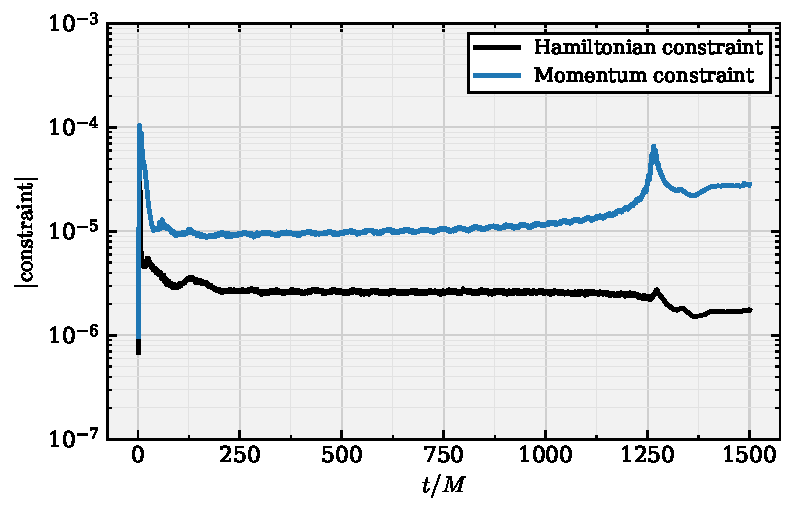
\includegraphics[width=0.65\textwidth]
{Figures/Chapter_2/Constraints/q1/emda_prof_Constraints_Hamiltonian_plus_MomentumSum.pdf}
\caption{
Hamiltonian and combined momentum-constraint violations for a
representative $q=1$ binary evolution. The constraints remain
controlled throughout the inspiral.
}
\label{fig:q1_constraints}
\end{figure}

\begin{figure}[t]
\centering
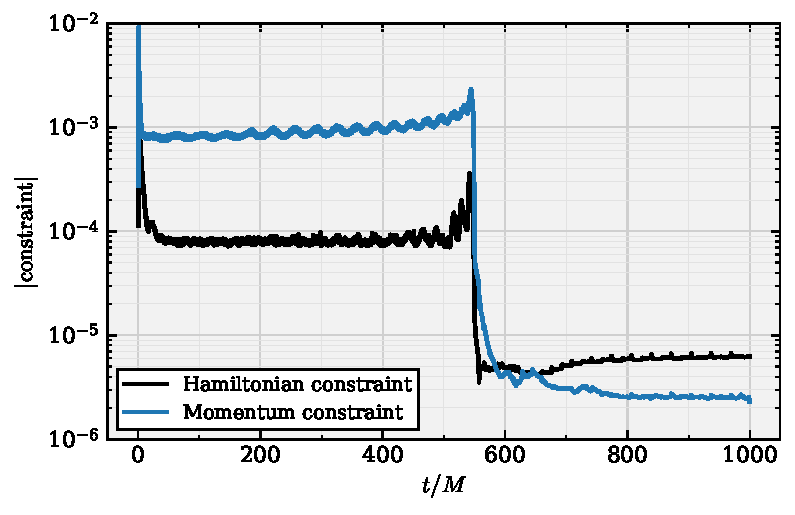
\includegraphics[width=0.65\textwidth]
{Figures/Chapter_2/Constraints/q8/emda_prof_Constraints_Hamiltonian_plus_MomentumSum.pdf}
\caption{
Hamiltonian and combined momentum-constraint violations for the
$q=8$ binary evolution. Although the unequal-mass system places
greater demands on the adaptive mesh, the constraints remain
bounded throughout the simulation.
}
\label{fig:q8_constraints}
\end{figure}



\chapter{Interpolating the EMDA Theory Space}
\section{Introduction}

The growing number of detected binary black hole mergers provides an increasingly broad sample of gravitational wave signals with which to test general relativity in the strong field, dynamical regime. Continued improvements to the LIGO, Virgo, and KAGRA detectors are expected to further increase the rate of observed compact binary mergers, expanding the available catalog of gravitational wave events \cite{GWTC3,GWTC4}. As this catalog grows, gravitational wave observations provide an increasingly powerful way to search for small deviations from general relativity and to constrain alternative theories of gravity \cite{Yunes2025GWTests,Yagi2016_BHTestsGR,Berti2015}.

Numerical relativity plays an important role in this effort because the merger regime is highly nonlinear and theory dependent. However, numerical relativity models for alternative theories of gravity are less mature than their general relativistic counterparts. Simulating such theories presents several challenges. Some modified theories suffer from pathologies such as evolution systems that are not well posed or ghostlike degrees of freedom associated with higher derivative terms \cite{PapalloReall2017,KovacsReall2020,Woodard2015}. Numerical studies of these theories therefore require formulations in which the initial value problem can be posed consistently and the subsequent evolution remains well behaved. In particular, one must construct suitable initial data and evolve the system in a way that controls the constraints.

Many tests of gravity can be understood as constraints on additional features that are absent in vacuum general relativity. For example, previous work has used gravitational wave observations to bound higher curvature corrections, placing limits on the length scales over which such terms can become important \cite{Nair2019,Perkins2021HigherCurvature,Yunes2025GWTests}. Other studies have considered constraints on black hole charge \cite{Bozzola2021,ferreira2026electromagneticdualitydegeneracydynamical}, as well as tests based on black hole shadows \cite{Sahoo2024PRD,Sahoo2025}. In this chapter, we investigate another possible extension: Einstein--Maxwell--dilaton--axion (EMDA) theory. EMDA theory contains, in addition to the metric and electromagnetic field, a scalar dilaton field and a pseudoscalar axion field. These additional degrees of freedom can modify the structure of charged black holes and may leave observable imprints on binary mergers and their emitted radiation \cite{Sen1992,Sen1995,Horne1992,Hirschmann2018}.

Analytic black hole solutions in theories related to EMDA are known for special choices of the coupling parameters. These include the Kerr--Sen black hole for $\alpha_0=\alpha_1=1$, Einstein--Maxwell--dilaton black holes for $\alpha_1=0$, and Kaluza--Klein black holes for $\alpha_0=\sqrt{3}$ \cite{Sen1992,Sen1995,Horne1992,Mignemi1993_ChargedStringBH}. To explore the broader theory space, we construct approximate initial data by scaling the scalar fields by their couplings and then solving the initial data problem. Although these data are not exact, they are expected to be close enough to the desired configuration that the black holes quickly relax toward a quasiequilibrium state early in the evolution. The stability of Kerr--Sen black holes has recently been studied in both perturbative and fully nonlinear settings \cite{PopeRohrerWhiting2025,Carroll2026KerrSenStability}, and previous numerical work has explored portions of the EMD parameter space using similar techniques \cite{Hirschmann2018}. However, less is known about how varying the EMDA coupling parameters affects the nonlinear dynamics of binary black hole mergers.

Here, we focus primarily on the $\alpha_0=\alpha_1$ part of the EMDA parameter space. By varying this common coupling, we study how the strength of the dilaton and axion interactions influences the merger dynamics and the resulting gravitational wave signals. This provides a first step toward understanding how binary black hole observations may constrain broader regions of EMDA theory beyond the analytically known special cases.

The goal of this chapter is not to produce a catalog level set of simulations. Instead, we use approximate charged binary black hole initial data to explore how the dynamics depend on the EMDA coupling parameters.

\section{Theory space}
\label{sec:theory_space}

As our starting point, we consider Einstein--Maxwell--dilaton--axion (EMDA) theory, in which the Einstein--Maxwell system is supplemented by a scalar dilaton field $\phi$ and a pseudoscalar axion field $\kappa$. The action is
\begin{equation}
\begin{aligned}
S = \int \mathrm{d}^4 x,\sqrt{-g}\Big[
&\frac{R}{8\pi}
-2\nabla_a\phi\nabla^a\phi
-e^{-2\alpha_0\phi}F_{ab}F^{ab} -\frac{1}{2}e^{4\alpha_1\phi}\nabla_a\kappa\nabla^a\kappa
-\kappa F_{ab}({}^{*}F)^{ab}
\Big],
\end{aligned}
\label{eq:emda_action}
\end{equation}
where $R$ is the Ricci scalar, $F_{ab}$ is the $U(1)$ field strength, and $(*F)_{ab}$ is its dual. The constants $\alpha_0$ and $\alpha_1$ determine the coupling strengths between the dilaton, axion, and electromagnetic field. In this chapter, we focus primarily on the one-parameter diagonal sector
\begin{equation}
\alpha_0=\alpha_1 .
\end{equation}

Different choices of $\alpha_0$ and $\alpha_1$ correspond to different members of this class of theories. The choice $(\alpha_0,\alpha_1)=(1,1)$ corresponds to the coupling values associated with the low-energy limit of heterotic string theory and admits the Kerr--Sen black-hole solution \cite{Sen1992,Sen1995}. Setting $\alpha_0 =1, \alpha_1=0$ gives an Einstein--Maxwell--dilaton-type system, with the Kaluza--Klein value corresponding to $\alpha_0=\sqrt{3}$ \cite{Horne1992,Mignemi1993_ChargedStringBH}. The case $(\alpha_0,\alpha_1)=(0,0)$ removes the exponential dilaton dependence from the Maxwell and axion kinetic terms and provides a useful reference point for comparison.

For the comparisons presented here, we consider the diagonal EMDA values
\begin{equation}
(\alpha_0,\alpha_1)=(0,0),\quad (1,1),\quad (10,10),\quad (100,100).
\end{equation}
We also include selected EMD benchmark cases,
\begin{equation}
(\alpha_0,\alpha_1)=(1,0),\quad (\sqrt{3},0),
\end{equation}
to compare the diagonal EMDA evolutions with representative dilatonic cases. These choices allow us to compare a weakly coupled reference case, the standard EMDA/Kerr--Sen coupling, two larger-coupling EMDA cases, and known EMD limits.

Analytic stationary black-hole solutions are not known for all of the coupling choices considered here. Moreover, even when stationary single-black-hole solutions are known, our binary configurations are constructed using approximate initial data rather than exact binary black-hole solutions. We therefore construct approximate charged binary black-hole initial data and evolve the full EMDA system numerically. During the early part of the evolution, the black holes and surrounding fields are allowed to relax dynamically before inspiral and merger.

This approach allows us to compare the resulting gravitational waveforms against a common reference waveform and to identify how the electromagnetic, dilaton, and axion fields influence the inspiral and merger dynamics. The known analytic black-hole metrics and associated fields relevant to this theory space are summarized in Appendix~\ref{sec:appx:SchwarzschildBH} with the Kerr-Sen black hole given in in an earlier chapter.

\section{Numerical Methods}

To study the strong-field dynamics and gravitational radiation from inspiraling charged black-hole binaries in Einstein--Maxwell--dilaton--axion theory, we evolve the full EMDA system as a Cauchy initial-value problem. The spacetime metric is evolved using the BSSN formulation \cite{Shibata1995_BSSN,Baumgarte1999_BSSN,Baumgarte2010}, together with puncture gauge conditions \cite{Campanelli2006,Baker2006}. The electromagnetic, dilaton, and axion fields are evolved using the matter evolution equations obtained from the $3+1$ decomposition of the EMDA equations of motion. The full evolution system is summarized in earlier chapters.
We use the same numerical code used in earlier chapters . In contrast to the head-on collisions considered there, the simulations presented here describe binary black holes with nonzero orbital angular momentum. We use the same assumptions and techniques to set the inititial data that we used in our chapter on inspirirlaing black holes. The black holes are assigned initial linear momenta chosen to approximate quasicircular inspiral. This allows us to follow the late inspiral, merger, and ringdown and to extract gravitational, electromagnetic, dilaton, and axion radiation from the resulting spacetime.

Because the initial data are approximate, the electromagnetic constraints do not vanish identically at the initial time. To control these constraint violations, we evolve the electromagnetic fields with hyperbolic divergence cleaning. In this approach, auxiliary damping fields propagate violations of the electric and magnetic constraints away from the strong-field region and damp them during the evolution \cite{Palenzuela2009}. This prevents electromagnetic constraint violations from accumulating during the relaxation, inspiral, and merger. The expected damping of the constraint equations is shown in Figure ~\ref{fig:chapter3_dive_constraint}

\subsection{Initial data}

Constructing initial data for binary black holes in EMDA theory is challenging because exact binary black hole solutions are not known. In addition, for general choices of the coupling parameters, the corresponding stationary single black hole solutions are not available in closed analytic form. We therefore use an approximate initial data prescription guided by the known Kerr--Newman and Kerr--Sen solutions \cite{Sen1992,Sen1995}.

Our starting point is a charged binary black hole configuration motivated by Kerr--Newman and constructed using approximate charged puncture data \cite{Bowen1980,Alcubierre2009,Bozzola2019}. We supplement these data with approximate dilaton and axion fields motivated by the Kerr--Sen solution. Since we are interested in varying the coupling parameters, we rescale the scalar and pseudoscalar fields according to the chosen coupling. In particular, for the diagonal choice $\alpha_0=\alpha_1$, we take the initial dilaton profile to scale with $\alpha_0$, so that larger coupling values correspond to larger initial scalar field amplitudes. For the dilaton, we therefore set
\begin{align}
    \phi = \alpha_0 \left[\phi_1(r_1,\theta_1) + \phi_2(r_2,\theta_2)\right].
\end{align}

This prescription does not produce an exact solution of the EMDA constraint equations. Instead, it should be viewed as an approximate data construction designed to place the system near the expected charged black hole configuration for each coupling choice. After the evolution begins, the black holes and surrounding fields are allowed to relax dynamically before the late inspiral and merger.

For each coupling choice, we consider binaries with charge to mass ratio magnitude $\lambda=Q/M=0.01$ and a small spin $\chi=0.2$. We examine three representative charge configurations: $++$, $+-$, and $+0$. In the $++$ case, both black holes carry charge with the same sign; in the $+-$ case, the black holes carry equal and opposite charges; and in the $+0$ case, only one black hole is charged. These configurations allow us to compare systems with different net charges and electromagnetic field structures while keeping the individual charge scale fixed.

We then use the subsequent evolution to study how changing the coupling strength affects the electromagnetic, dilaton, and axion fields, the binary dynamics, and the emitted gravitational radiation.

\section{Results}

\subsection{Waveform comparison}

\paragraph{Gravitational waves}

We first compare the gravitational waveforms produced by the different coupling choices. For this comparison, we use the Einstein--Maxwell case, $(\alpha_0,\alpha_1)=(0,0)$, as the reference waveform and compare the dominant $(\ell,m)=(2,2)$ mode against the corresponding modes from the EMD and EMDA evolutions.

For the charge considered here, the gravitational waveforms remain close to the Einstein--Maxwell reference waveform across all of the coupling choices. In most cases, the differences in the dominant strain are too small to interpret as clearly resolved coupling-dependent effects. Because the simulations use approximate initial data, the early relaxation of the black holes and surrounding fields can introduce waveform differences that are unrelated to the intended change in the coupling parameters. These effects, together with finite-resolution error, waveform-extraction error, and the short duration of the evolutions, likely dominate the very small differences observed among most of the runs.

The main robust conclusion is therefore qualitative. For the smaller-coupling EMD and EMDA cases, the dominant gravitational waveform is effectively indistinguishable from the Einstein--Maxwell reference waveform at the accuracy of the present simulations. The strongest-coupling case, $(\alpha_0,\alpha_1)=(100,100)$, produces the largest departure from the reference waveform. Even in this case, however, the dominant strain remains close to the Einstein--Maxwell waveform.

These results suggest that, for the relatively small charge considered here, coupling-dependent effects in the dominant gravitational-wave mode are subtle. Larger charges, longer inspirals, improved initial data, and explicit convergence tests may be required to separate physical coupling-dependent effects from relaxation and numerical errors. The present comparisons should therefore be interpreted as an exploratory test of the EMDA coupling dependence rather than as precision estimates of waveform distinguishability.

Figure~\ref{fig:em_vs_emda_hplus} shows a representative comparison between the Einstein--Maxwell reference waveform and the strongest-coupling EMDA case. The two waveforms are peak-aligned, there is almost no difference in the wavefrom.
\begin{figure}[t]
\centering
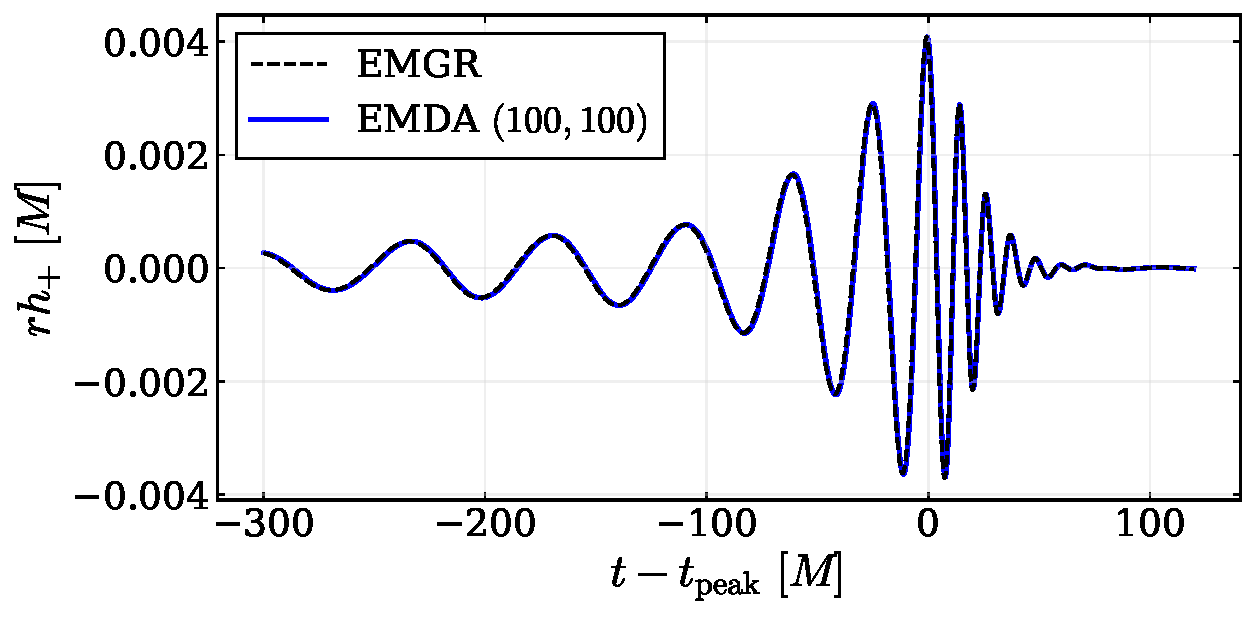
\includegraphics[width=0.85\textwidth]{Figures/Chapter3/em_a0_0_a1_0_vs_emda_a0_100_a1_100_peak_aligned_hplus_notitle.pdf}
\caption{Peak-aligned comparison of the dominant gravitational-wave strain between the Einstein--Maxwell reference waveform, $(\alpha_0,\alpha_1)=(0,0)$, and the strongest-coupling EMDA case, $(\alpha_0,\alpha_1)=(100,100)$. The waveforms agree extremely well, the mismatch of this waveform is on the order of $10^{-5}$}
\label{fig:em_vs_emda_hplus}
\end{figure}
 
\paragraph{Electromagnetic radiation}

We also compare the electromagnetic radiative modes and $\Phi_2$, as introduced in earlier chapters. Rather than computing a mismatch for these modes, we perform a direct comparison of the electromagnetic waveforms. The results show that the waveform differences increase as the coupling strengths are increased. The electromagnetic signal retains the same basic structure across the coupling choices, but its amplitude changes. We display the $++$ charge configuration here, although the other charge configurations show broadly similar behavior.

\begin{figure}[t]
\centering
\subfloat[Real part of $\Phi_2^{22}$.]{
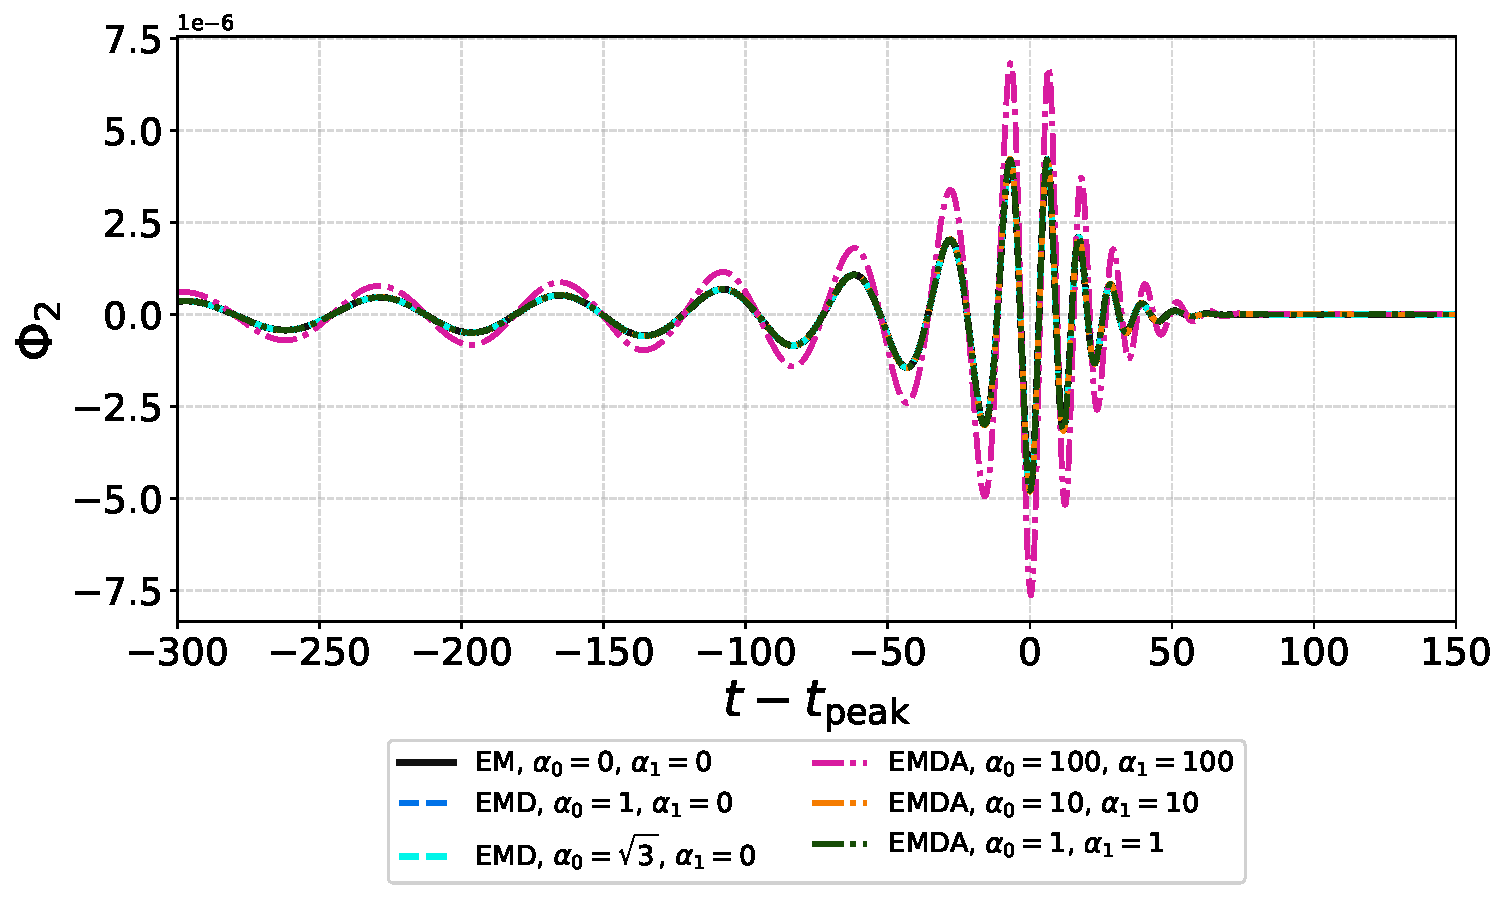
\includegraphics[width=0.48\textwidth]{Figures/Chapter3/PHI2_l2_m2_r5_real.pdf}
}
\hfill
\subfloat[Absolute difference relative to the Einstein--Maxwell case.]{
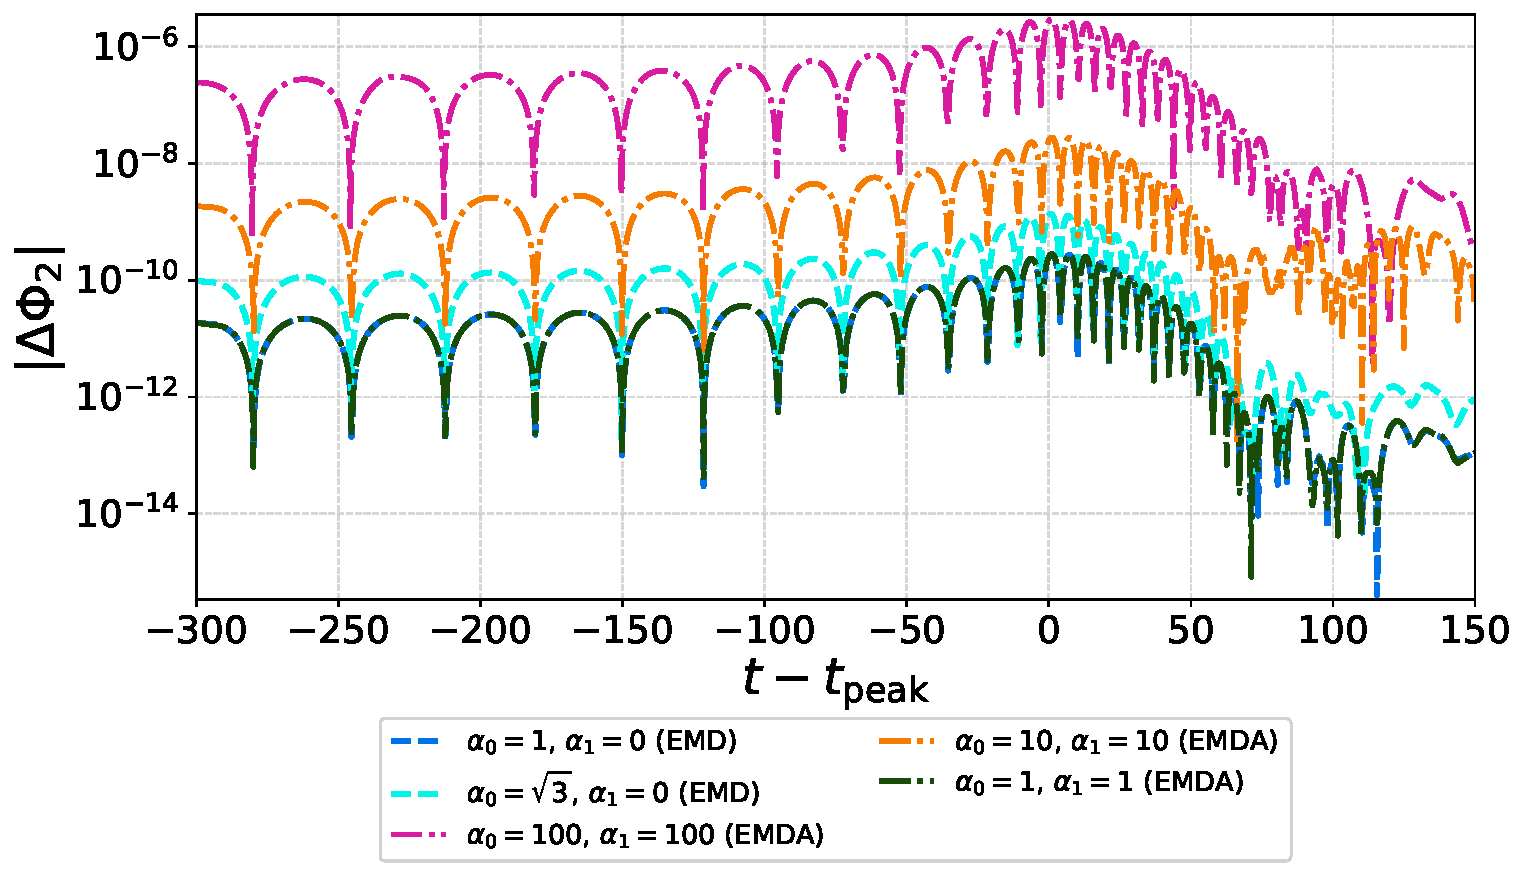
\includegraphics[width=0.48\textwidth]{Figures/Chapter3/PHI2_l2_m2_r5_real_absdiff_vs_EM_log.pdf}
}
\caption{Comparison of the $(\ell,m)=(2,2)$ mode of the electromagnetic scalar $\Phi_2$, extracted at $R_{\mathrm{ex}}=100M$. The left panel shows the peak aligned real part of $\Phi_2^{22}$ across the coupling choices considered, while the right panel shows the absolute difference relative to the Einstein--Maxwell reference case, $(\alpha_0,\alpha_1)=(0,0)$, on a logarithmic scale. The differences in the waveform get larger as the coupling is increased, although it is primarily the amplitude that changes.}
\label{fig:phi2_l2m2_ch3}
\end{figure}


\paragraph{Dilaton radiation}

\begin{figure}[t]
\centering
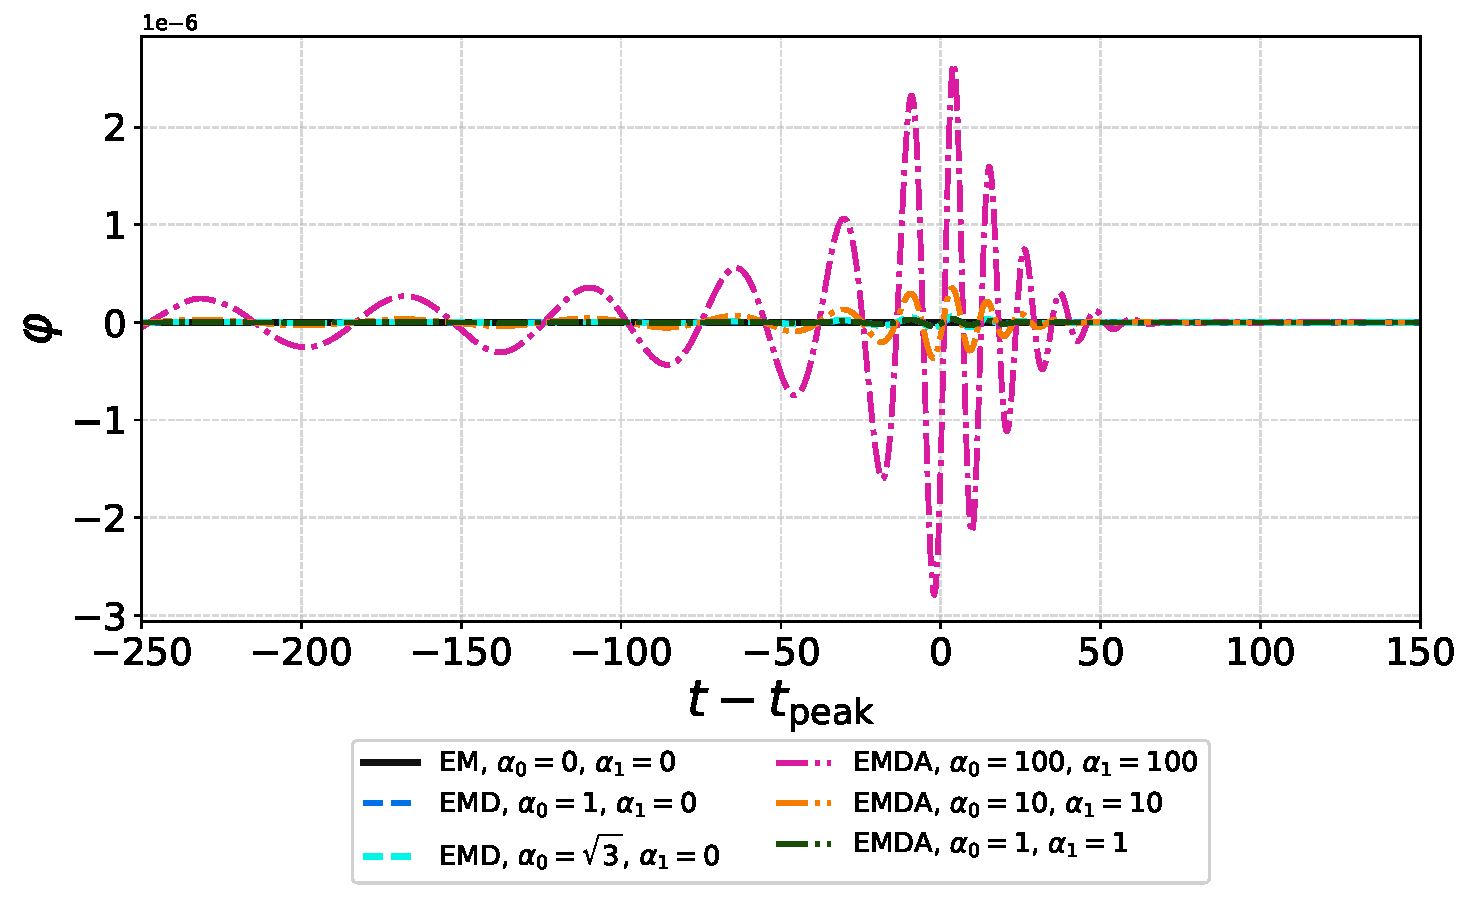
\includegraphics[width=0.48\textwidth]
{Figures/Chapter3/Dilaton_l2_m2_r5_real.pdf}
\caption{
Peak-aligned comparison of the real part of the
$(\ell,m)=(2,2)$ mode of the dilaton radiation,
extracted at $R_{\mathrm{ex}}=100M$, for the coupling
choices considered.
}
\label{fig:dilaton_l2m2_ch3}
\end{figure}

As the coupling strength increases, the amplitude of the emitted
dilaton radiation also increases.


\subsection{Constraints}

Because the initial data are approximate, the constraint violations provide an important check on the quality of the evolutions. We monitor the Hamiltonian constraint, together with the electric and magnetic divergence constraints, throughout the simulations. These quantities are shown in Figs.~\ref{fig:chapter3_hamiltonian_constraint}--\ref{fig:chapter3_divb_constraint}. Across the set of coupling choices considered here, the constraints remain controlled during the initial relaxation, inspiral, and merger. The largest features occur during the early relaxation phase and near merger, where the fields vary most rapidly.

\begin{figure}[t]
\centering
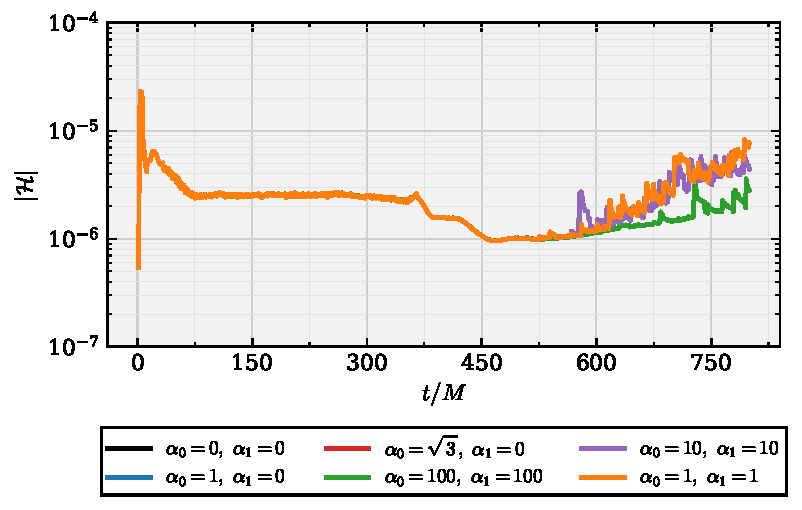
\includegraphics[width=0.85\textwidth]{Figures/Chapter3/all_runs_C_HAM.pdf}
\caption{Hamiltonian constraint violation for the different coupling choices. The curves show the evolution of the Hamiltonian constraint norm for the Einstein--Maxwell reference case and the corresponding EMD and EMDA evolutions. There is an initial spike as the simulations begin, but the constraint quickly settles to a lower value. The Hamiltonian constraint does not show runaway growth and remains low throughout the evolution.}
\label{fig:chapter3_hamiltonian_constraint}
\end{figure}

\begin{figure}[t]
\centering
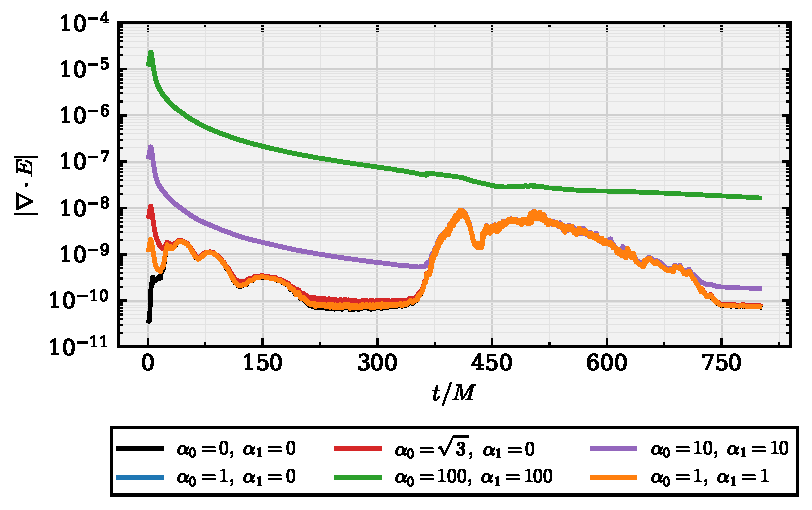
\includegraphics[width=0.85\textwidth]{Figures/Chapter3/all_runs_C_DIVE.pdf}
\caption{Electric divergence constraint violation for the different coupling choices. The curves show the evolution of the electric constraint norm across the Einstein--Maxwell, EMD, and EMDA evolutions. The constraint is initially largest for the strongest coupling, but hyperbolic cleaning reduces it over time. Overall, these constraints remain well behaved throughout the evolution.}
\label{fig:chapter3_dive_constraint}
\end{figure}

\begin{figure}[t]
\centering
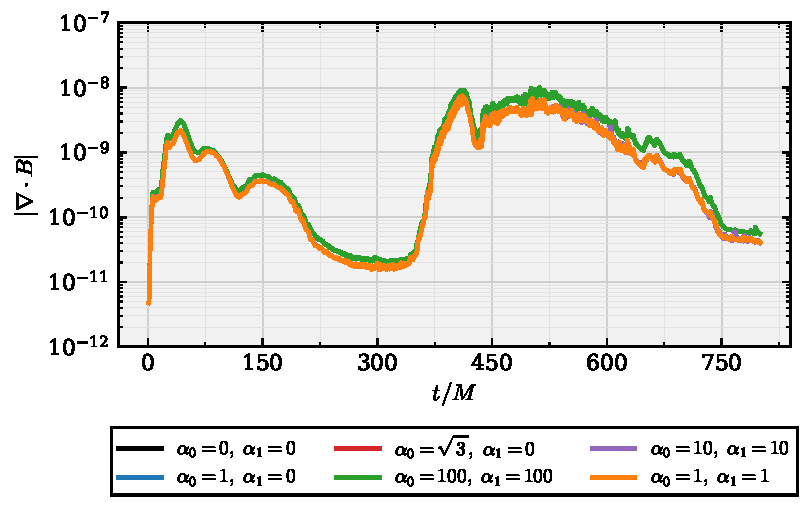
\includegraphics[width=0.85\textwidth]{Figures/Chapter3/all_runs_C_DIVB.pdf}
\caption{Magnetic divergence constraint violation for the different coupling choices. The curves show the evolution of the magnetic constraint norm across the Einstein--Maxwell, EMD, and EMDA evolutions. These values remain low throughout the simulation, providing confidence that the magnetic divergence constraint remains well behaved.}
\label{fig:chapter3_divb_constraint}
\end{figure}

The electromagnetic constraints remain bounded throughout the evolutions, indicating that the divergence-cleaning scheme prevents the electric and magnetic constraint violations from growing without bound. The Hamiltonian constraint shows the expected transient behavior during the initial relaxation and near merger, but it does not exhibit runaway growth. These results indicate that the simulations remain sufficiently well controlled for the qualitative waveform comparisons presented above.

\section{Conclusion}

In this chapter, we studied binary black hole mergers in a broader region of Einstein--Maxwell--dilaton--axion theory by varying the coupling parameters that control the interactions between the electromagnetic, dilaton, and axion fields. We focused primarily on the diagonal sector, $\alpha_0=\alpha_1$, and compared several representative coupling choices against the Einstein--Maxwell reference case. Because exact binary black hole initial data are not available for these theories, we used approximate charged binary black hole initial data and allowed the systems to relax dynamically before merger.

The evolutions remained stable for the coupling choices considered here, and the electromagnetic and gravitational constraints remained controlled throughout the simulations. This provides evidence that the numerical framework can be used to explore binary black hole dynamics beyond the analytically known special cases of EMDA theory. In particular, these simulations provide a first step toward studying how nonlinear merger dynamics depend on the theory's coupling parameters.

For the small charge considered in this study, we found that the dominant gravitational wave signal is only weakly affected by the choice of coupling. The smaller coupling EMD and EMDA cases remained effectively indistinguishable from the Einstein--Maxwell reference waveform at the accuracy of the present simulations. The strongest coupling case, $(\alpha_0,\alpha_1)=(100,100)$, produced the largest departure from the reference waveform, but even this difference remained small in the dominant strain.

The electromagnetic radiation shows a clearer dependence on the coupling parameters. Rather than computing electromagnetic mismatches, we directly compared the radiative modes $\Phi_2$ against the Einstein--Maxwell reference case. These comparisons show that the electromagnetic waveform differences generally increase as the coupling strengths are increased. The overall structure of the electromagnetic signal remains similar across the coupling choices, but the amplitude changes. This behavior is shown for the $++$ charge configuration, with the other charge configurations exhibiting broadly similar patterns.

Taken together, these results suggest that coupling dependent effects are subtle in the gravitational radiation at small charge, but are more visible in the electromagnetic sector. Because the simulations use approximate initial data, very small waveform differences may be affected by relaxation effects, finite resolution error, and waveform extraction uncertainty rather than only by physical coupling dependence. Larger charges, longer inspirals, improved initial data, and explicit convergence tests may be required to clearly separate physical effects from numerical and initial data uncertainties.

Future work could potentially look at improving the initial data by adding axion contributions and improving the initial electric field used in the TPID solver. We could also perform higher charge or higher spin runs to test a wider range of Kerr--Sen configurations. Another study could examine different parts of the EMDA parameter space, including cases where the two couplings are not equal, $\alpha_0 \neq \alpha_1$.

\subsection{Mismatch summary}

\begin{table}[t]
\centering
\begin{tabular}{lccc}
\hline
Theory & $q=0.05,\,+0$ & $q=0.05,\,+-$ & $q=0.05,\,++$ \\
\hline
EMD $(\alpha_0,\alpha_1)=(1,0)$
& $3.85\times 10^{-8}$
& $2.70\times 10^{-7}$
& $4.43\times 10^{-14}$ \\
EMD $(\alpha_0,\alpha_1)=(\sqrt{3},0)$
& $3.53\times 10^{-12}$
& $9.00\times 10^{-8}$
& $2.89\times 10^{-12}$ \\
EMDA $(\alpha_0,\alpha_1)=(1,1)$
& $2.59\times 10^{-8}$
& $6.08\times 10^{-8}$
& $4.92\times 10^{-14}$ \\
EMDA $(\alpha_0,\alpha_1)=(10,10)$
& $7.06\times 10^{-8}$
& $1.22\times 10^{-6}$
& $6.14\times 10^{-10}$ \\
EMDA $(\alpha_0,\alpha_1)=(100,100)$
& $9.62\times 10^{-6}$
& $4.42\times 10^{-5}$
& $3.91\times 10^{-6}$ \\
\hline
\end{tabular}
\caption{Mismatch between the Einstein--Maxwell reference waveform, $(\alpha_0,\alpha_1)=(0,0)$, and the waveforms obtained for different coupling choices. The comparisons use the dominant $\ell=m=2$ gravitational strain mode. The mismatches are small, so most of these waveforms should be considered effectively indistinguishable within the accuracy of the present simulations. In this regime, finite resolution, approximate initial data, and other numerical effects may contribute more to the measured mismatch than the scalar and pseudoscalar fields themselves.}
\label{tab:emda_coupling_mismatches}
\end{table}

\chapter{Compact Finite Difference Operators for Adaptive Simulations}
\section{Introduction}
\label{sec:intro}

The last decade has seen dramatic growth in the field of gravitational wave astronomy~\cite{Abbott2016b,GWTC1,GWTC2,GWTC3,GWTC4,GWTC5}. LVK has discovered the gravitational wave signals from nearly four hundred compact mergers, the majority being binary black hole mergers~\cite{GWTC5}.  Additional detections will continue to be made and new gravitational wavebands will open up with planned and proposed gravitational wave detectors~\cite{Maggiore2020_ET,Reitze2019_CosmicExplorer,Evans2021_CEHorizon}.  With these, there will come an increasing need for more comprehensive and ever more accurate simulated gravitational waveforms~\cite{Lindblom2008AccuracyStandards,Purrer2020_AccuracyRequirements,Jan2024AccuracyLimitations}.  

While the exact level of precision required is not entirely clear, there is broad agreement that significant improvements in simulation fidelity will be required~\cite{Lindblom2008AccuracyStandards,Purrer2020_AccuracyRequirements,Jan2024AccuracyLimitations}.
For example, future gravitational wave detectors such as
LISA, Einstein Telescope, and Cosmic Explorer will have higher signal-to-noise
ratios than current detectors~\cite{Maggiore2020_ET,Reitze2019_CosmicExplorer,Evans2021_CEHorizon}. This will increase accuracy requirements
for simulated waveforms; some estimates suggest by as much as two orders of
magnitude~\cite{Ferguson2021_Readiness,Purrer2020_AccuracyRequirements,Jan2024AccuracyLimitations,Thompson2025_Indistinguishability}.
While there are some ideas~\cite{Fernando2019,Fernando2023,Black2025_ORBIT,Etienne2024,Assumpcao2022_HyperbolicRelaxation,Tootle2025,Lele1992,Daszuta2024} of how to improve the efficiency and accuracy of current codes, the size of the hoped for increase is daunting.
%Attaining this will be difficult but several avenues are possible to move towards greater waveform accuracy.

Current numerical relativity codes run on CPUs have probably wrung about as much
efficiency and time savings as possible from standard finite difference
and finite volume techniques.  Adaptive methods have become fairly state-of-the-art
and a number of codes have adopted octree partitioning to improve
the distributed aspects of binary inspiral calculations~\cite{Fernando2019,Fernando2023,Radia2022_AMR,Rashti2024_AMR,Daszuta2024_AdaptiveMeshes}.  It is natural to ask
where accuracy
improvements for waveform simulation might come from.  Two possible areas
where improvements in accuracy may be obtainable include moving to GPUs to speed up calculations and using improved, higher order accuracy algorithms~\cite{Lewis2018_GPU,Tootle2025,AthenaK2024_NR,Lele1992,Daszuta2024}.  A number of groups and codes have begun to develop for GPUs as have we~\cite{Fernando2019}.  But in this work we will focus on the latter of these, namely higher accuracy finite
differencing schemes in the form of compact finite differences (CFDs)~\cite{Lele1992,Kim2007,Kim2010,Kim2013,KimSandberg2012,Daszuta2024,WuKim2024}.


To the best of our knowledge, the first use of CFD operators in numerical
relativity was by Daszuta~\cite{Daszuta2024}.  His implementation
focused on costs associated with communication across many processors and,
partly in consequence of that, was not entirely satisfactory as it did not
demonstrate the hoped for performance gains.
Nonetheless, CFDs have been used for over thirty years in the engineering
literature~\cite{Lele1992,Kim2007,WuKim2024,VisbalGaitonde2002,BradyLivescu2019} with impressive accuracy improvements
in the simulation of both linear and nonlinear systems of equations.  So one might think that use of these in numerical relativity may be one route to improved accuracy in binary simulations and the gravitational radiation they source.

Our aim in the current work is to develop high order compact finite difference schemes together with boundary closures and test them on linear and nonlinear time evolution systems in three dimensions.
Indeed, we are able to demonstrate the utility of these schemes and that, in the test cases considered here, an increase in the effective order of accuracy is possible.


%The paper is structured as follows.  ... 
The paper is structured as follows. Section~II provides background on compact finite difference schemes and discusses their advantages relative to explicit finite difference methods, together with the challenges associated with boundary closures and stability. Section~III describes the construction and optimization of the first derivative operators, including the treatment of interior and boundary stencils and the resulting fourth and sixth order schemes. Section~IV presents the corresponding construction of compact operators for second derivatives. In Sec.~V, we test the operators on a sequence of linear and nonlinear systems, including the classical wave equation, Maxwell's equations, Burgers' equation, the nonlinear sigma model, and Teukolsky gravitational wave evolutions using the BSSN equations. Finally, Sec.~VI summarizes our results and discusses future applications of compact finite differences in numerical relativity.

\section{Background}
\label{sec:background}

Finite difference (FD) schemes are widely used in numerical relativity.  This is partly due to their simiplicity and relative ease of implementation. Unfortunately,
higher order FD schemes require large stencils, particularly when shifted stencils near boundaries may be required.  In a given implementation, this can lead to a large spread in memory access.  In general, this will 
complicate numerical treatments near boundaries and increase 
communication costs for ghost regions at both processor and refinement boundaries~\cite{Fernando2019,KimSandberg2012,Kim2013,Daszuta2024}. 
As such, seeking higher accuracy gravitational waveforms using standard FDs would appear to incur increasing compute costs and thereby compromise those hoped for gains.

Compact finite difference (CFD) schemes are a generalization of Pad\'e approximates~\cite{Lele1992}
that couple derivatives at neighboring points at different spatial scales.
In general, for a fixed stencil size, these will be higher-order than standard FD schemes~\cite{Lele1992,Kim2007,Daszuta2024}.  When compared to explicit FDs, compact schemes of similar order require
smaller stencils and can be significantly
more accurate--often by a factor of 10--100$\times$ more accurate~\cite{Lele1992,Kim2007,Wang2018,Daszuta2024}.  
A price to pay for this increase in accuracy is that CFD schemes are
implicit and therefore require matrix inversion~\cite{Lele1992,Kim2013,KimSandberg2012}.  However, our use of \dendrogr\
permits us to partially sidestep this issue~\cite{Fernando2019,Fernando2023}.  In particular, 
\dendrogr's leaf nodes are of fixed size, and using
vectorized libraries for matrix inversion gives an
efficient calculation of CFDs that, we have found, are as fast as
hand-coded \texttt{C++} code for explicit FDs.  %\eric{Can someone double check my claim here that I am not overstating anything.  A reference would also be nice if we have it.}

We here describe the development and evaluation of new families of CFD operators appropriate
for use within distributed numerical relativity codes using adaptive meshes.
This has required the careful consideration of two crucial issues, namely appropriate
boundary closures for these CFD operators and the question of stability of the
operators for both linear and nonlinear systems of equations.

%In addition to physical boundaries, the use of adaptive meshes naturally
%introduces refinement boundaries in the interior of the domain. 

For finite difference (or finite volume) based
approaches, the stencil that defines derivative approximations will necessarily
be different between the ``interior" of the mesh and near the boundaries of the mesh.  These boundaries can include physical boundaries as well as, in the case of adaptively refined meshes, refinement boundaries.  
%(whether refinement, physical, or otherwise).
Typically, shifted FD stencils together with some form of interpolation are used in the vicinity of either type of boundaries.  However, this can 
introduce larger errors than those expected from uniform, centered approximations.
Such remains true for CFDs.  Following an ingenious approach of
Wu and Kim~\cite{Kim2007,WuKim2024}, we have developed CFD operators for both first and
second derivatives with boundary closures which use a high order interpolating
polynomial to permit the continued use of centered-like stencils at and near
boundaries.   We have generalized this method to include a set of free parameters in the specification of the CFD operators.  Together with the use of spectral error quantities associated with both interior and boundary operators, we minimize the error with respect to the free parameters thereby allowing the construction of optimized families of CFD operators for a fixed order of accuracy.  

The stability of the resulting families of CFD operators is then determined
in two complementary ways.  A version of linear stability is defined with
respect to a simple advection (for first derivatives) or wave equation (for
second derivatives)
by considering the eigenvalue spectrum of the operator.
Given our definitions, the linear stability of a CFD derivative is established
if all the eigenvalues are restricted to a portion of the complex frequency
plane (left half plane for first derivatives and lower half plane for second
derivatives).

The operators are then further tested in  simpler
model systems of equations, such as Maxwell's equations.
Normed error quantities
are monitored and checked that the CFD operators do, indeed, produce stable
evolutions.

%\begin{wrapfigure}{r}{0.55\textwidth}
%    \centering
%    \includegraphics[width=0.55\textwidth]{figs/Bz_error_first_deriv_CFDs.pdf}
%    \vspace{-.75cm}
%    \caption{\small Error curves for the $z$ component of the magnetic field for a propagating dipole using both CFDs and standard FDs at different resolutions on a uniform grid.  A4 and C4 are examples of fourth order CFDs developed for \dendrogr.  WuKim is a fourth order CFD developed by~\cite{WU2024112887}.  E4 and E6 are explicit FD operators.  Two takeaways are that the CFDs exhibit an error profile comparable to the sixth order explicit operators and, even more significantly, the CFDs at nominal fourth order accuracy are comparable to the fourth order explicit FDs at half the resolution.}
%\label{fig:prior_cfd}
%\end{wrapfigure}

As a result, we have found families of stable, fourth and sixth order accurate,
boundary closed operators. They demonstrate improved accuracy over their
explicit counterparts, as shown in
Fig.~\ref{fig:maxwell_fourth_order_error}. This figure shows the errors in the
$x$ components of the magnetic and electric fields for the evolution of a
magnetic dipole wave using a first order in time, first order in space
formulation of the Maxwell equations. Several fourth order compact and
explicit finite difference operators are compared at different resolutions.
The key results are that the nominally fourth order compact operators produce
error profiles comparable to those of the sixth order explicit scheme and,
more significantly, perform comparably to the fourth order explicit scheme
when run at half the resolution.

Comparable improvements are obtained for the sixth order first derivative
operators, as shown in Fig.~\ref{fig:maxwell_sixth_order_error}. Although the
sixth order compact operators do not achieve the full factor of two improvement
in resolution observed for the fourth order operators, they still reduce the
error by approximately an order of magnitude relative to the sixth order
explicit scheme. Similar behavior is also observed in the nonlinear sigma
model and Teukolsky wave tests presented below.





%\subsubsection{Compact Finite Differences}

%As explained in Section~\ref{sec:prior_cfd},  we have tested CFD operators
%in model problems using the Maxwell equations. In comparisons with
%explicit FD schemes, we have  demonstrated accuracy improvements of one to two
%orders of magnitude in the solutions.   We will extend these methods
%for use in solving the Einstein equations with \dendrogr.  To
%be successful, we will consider the following issues.

%CFD operaters were first used in numerical relativity by
%Daszuta~\cite{Daszuta:2023qdm}, however this implementation was not completely
%satisfactory and did not provide the expected performance
%gains.
%More generally, most CFD operators derived with linear stability
%conditions and periodic boundaries are unstable when applied to
%non-dissipative initial boundary value problems.
%However, Brady and Livescu recently developed a nonlinear
%optimization procedure to identify

%stable CFD operators~\cite{BRADY201984}.  We are now using their procedure
%to construct second-derivative CFD operators for numerical
%relativity.\footnote{Quite unexpectedly, the Maxwell equations
%with Dirichlet and Neumann boundary conditions are an acid test
%for the stability of CFD operators. Indeed, the only CFD
%operators that passed our long-term stability tests were the
%Brady-Livescu operators, which require no dissipation.
%The centered (unbiased) Daszuta operators, for these boundary
%conditions, were all unstable in these long-term tests.}

%One challenge with using CFD operators in the context of
%distributed computing, especially with different refinement levels,
%is minimizing potentially
%large numerical errors at refinement and domain boundaries,
%see, e.g., Ref.~\cite{Daszuta:2023qdm, KIM2013168}.
%Recent work by Wu and Kim significantly reduces this error
%using a boundary extrapolation method~\cite{WU2024112887}.  We will collaborate
%with Kim to include this technique in \dendrogr\ to
%ameliorate these errors (see letter of support).

%Another challenge concerns the fact that the black hole puncture hides the singularity, but the metric
%functions at this point are not smooth.
%Explicit FD about the puncture have unphysical oscillations,
%which, because they are well inside the horizon, are not
%problematic.  CFDs are coupled in a linear system, however,
%and unphysical oscillations are not isolated in space.
%Fortunately, WENO CFD operators are available for
%compressible fluids with shocks~\cite{LIU2015133,Ghosh_weno,SUBRAMANIAM2019108822}, which we can employ locally about the
%punctures. (BH locations are tracked at each step of the evolution.)
%Alternatively, high-order explicit derivatives could also be
%used locally about the puncture.

%Finally, the multi-scale nature of CFD requires solving
%a linear system for the coupled derivatives.  This does require
%additional computational overhead when compared with explicit schemes,
%but the cost is relatively small.  First, most CFD operators require
%only solving a tridiagonal system, which can be solved directly.

%Second, the equations of motion in \dendrogr\ are solved on the
%leaf nodes of the octree, which all have the same size.  Thus,
%the matrix CFD operator can be inverted one time on a leaf node, and then
%applied on all others, independent of resolution level.
%Finally, matrix operations on GPUs are very efficient.  Recalling
%the previous section, we will implement these new operators to run on GPUs.
%On current Nvidia GPUs, these can perform up to 256 matrix
%multiplications (GEMMs) per clock cycle on $4 \times 4$ matrices. The
%derivatives and RHS equations will need to be modified to make use of
%these cores, but promise tremendous speedups if successfully transformed.
%With these developments we expect to have stable CFD operators and improved boundary treatments resulting in an accuracy gain of an order of magnitude with little extra computational cost.

%We will update our code-generation framework to produce code that is capable
%of utilizing the tensor cores on modern GPUs.



% \eric{This next paragraph can probably be pulled; certainly from the dissertation and probably the paper.}
% To this point, our development of stable, boundary-closed CFDs has mostly been
% done using linear systems, such as the Maxwell equations. We have also tested
% the operators with a Schwarzschild black hole using the
% one-dimensional BSSN equations in spherical coordinates.
% As part of this  project we will extend this work to the Einstein equations,
% beginning with linearized gravitational waves.
% %We expect much of this testing to be accomplished
% %within the first six months of the grant period.

% \eric{The next paragraph should be pulled or put much later.}
% Based on some preliminary tests, our expectation is that accuracy improvements from
% using CFDs should largely carry over from the linear case to nonlinear settings.
% However, an additional issue that will require further exploration is the effect
% of the black hole puncture on the evolution when an implicit scheme such as CFDs
% are used.  While the black hole punctures effectively hide the singularities from
% the evolution it remains the case that the metric functions are not smooth there.
% Explicit FDs about the puncture will incur unphysical oscillations in the vicinity
% of the punctures, but because they are inside the horizon are not problematic.
% We have tested the use of CFDs in black hole spacetimes with a puncture
% by evolving a Schwarzschild black hole in extended spherical coordinates (along the
% axis for $\theta=\pm\pi/2$).  The use of adaptive stencils about the puncture

%with filtering allows to use CFDs in black hole spacetimes without loss of accuracy.

% \eric{This should probably be pulled as well.}
% While some testing of this has been done with initially promising results (we
% can do a head-on collision of a nonspinning equal mass BBH with boundary-closed
% first and second derivative CFDs), we still need to test more extensively the
% effect on accuracy in this more stringent setting.  Once such testing is done and we have confirmed accuracy improvements in
% \dendrogr\ with the use of these families of CFDs, we will compare older
% runs with mass ratios $q=2,4,8$ and $16$ against newer versions of such
% runs using CFDs.  

% Early indications of the accuracy improvements possible suggest that replacing an
% explicit FD with a CFD of the same nominal accuracy results in an evolution with
% comparable error at half the resolution (see Figure~\ref{fig:maxwell_fourth_order_error}).  For a time dependent problem across a 3D grid, this could result in
% a potential speedup or efficiency boost of up to $16\times$.  Indeed, in the aerospace community, there is a rule of thumb that the use of CFDs can result in a factor of $10\times$ improvement even for complex, nonlinear fluid flows.  \eric{Do we have a reference -- is it a personal communication with Kim?}  In the event that we don't realize
% exactly these same performance gains in the nonlinear Einstein equations, we still think that we can make a conservative estimate that the use of CFDs should give us at least a factor $2\times$ improvement.  Coupling this with speedups of $> 2\times$ that we have already seen from an earlier version of our GPU code~\cite{Fernando2019}, should
% allow a class of such BBH evolutions to be evolved that have heretofore been
% inaccessible (see Figure~\ref{fig:time}).

% %in cfd aerospace community there is a rule of thumb of a 10x improvment
% %if you don't believe ut we will scale back and consider 2x from CFDs and another 2x
% %from GPUS (that we have already done).





Early indications of the accuracy improvements possible suggest that replacing an
explicit FD with a CFD of the same nominal accuracy results in an evolution with
comparable error at half the resolution (see Figure~\ref{fig:maxwell_fourth_order_error}).  For a time dependent problem across a 3D grid, this could result in
a potential speedup or efficiency boost of up to $16\times$.  Indeed, in the aerospace community, there is a rule of thumb that the use of CFDs can result in a factor of $10\times$ improvement even for complex, nonlinear fluid flows.In the event that we don't realize
exactly these same performance gains in the nonlinear Einstein equations, we still think that we can make a conservative estimate that the use of CFDs should give us at least a factor $2\times$ improvement.  Coupling this with speedups of $> 2\times$ that we have already seen from an earlier version of our GPU code~\cite{Fernando2019}, should
allow a class of such BBH evolutions to be evolved that have heretofore been
inaccessible (see Figure~\ref{fig:walltime}).

%\section{First-derivative operators}
%\label{sec:first_der}
\section{Constructing CFD Operators}
\label{sec:constructing_CFDs}

\subsection{First derivative operators}
\label{sec:first_der}

We begin by reviewing the construction of high order, compact finite difference (CFD) schemes. 
The basic idea behind CFDs is a straightfoward generalization of a standard, explicit, centered finite difference stencil, such as that for the fourth order approximation of the first derivative 
\begin{equation}
    f_i' = \frac{1}{12h} \bigl[ f_{i-2} - 8 f_{i-1} + 8 f_{i+1} - f_{i+2} \bigr] + {\cal O}(h^4) , 
\end{equation}
\label{explicit}
to include values of the derivative at nearby grid points.  For example, one such generalization might be 
\begin{equation}
    \alpha_2 f_{i-2}' + \alpha_1 f_{i-1}' + f_i' + \alpha_1 f_{i+1}' + \alpha_2 f_{i+2}' = {1\over 2h} \Bigl[ a_1 ( f_{i+1} - f_{i-1} ) + a_2 ( f_{i+2} - f_{i-2} ) \Bigr] + {\cal O}(h^{2n}) 
\label{eighth_order_cfd}
\end{equation}

where the constant coefficients, $\alpha_1, \alpha_2, a_1$ and $a_2$ can be found be demanding a particular order of accuracy for the approximation ($2n$ in this example).  In this case, by matching Taylor coefficients, up to an eighth order scheme ($n=4$) may be defined with four linear conditions on the four coefficients.    

Similar such interior schemes are readily obtained.  Note that one need not solve for all of the coefficients so that some may be left as free parameters thereby becoming subject to conditions other than the order of accuracy of the scheme.  

Potential complications include the treatment of boundaries and that we have begun our illustration with a 1D example.  We will consider boundaries below.  As for considering this in higher dimensions, the extension is straightforward.  

%In systems of interest to us, such as the Einstein equations a serious issue arises associated with boundary

As our intent is to approximate a first derivative, $f'(x)$.  we assume a uniform grid in 1D with $N+1$ points and spacing $h$.  The earlier example can now be generalized to the following matrix system:
\begin{equation}
P_{ij} f_j' = {1 \over h} Q_{ij} f_j
\end{equation}
where $f_j$ is the vector of function values, $f_j'$ the vector of derivative values, and the matrices $P_{ij}$ and $Q_{ij}$ define the nature of the coupling between neighboring derivative and function values, respectively.  Of course, for an explicit finite difference scheme $P$ would be the identity.  Anything else will constitute some form of what we will refer to as a compact finite difference scheme.  
As in the example above, the interior points 
%Assuming a finite grid, the so-called ``interior points" of the scheme 
are straightforwardly obtained by matching the coefficients of a Taylor expansion of both sides in powers of the grid spacing $h$.  For the interior points, we always choose centered stencils similar to  to use centered stencil such as that in Eq.(\ref{eighth_order_cfd})
%\begin{equation}
%    \beta f_{i-2}' + \alpha f_{i-1}' + f_i' + \alpha f_{i+1}' + \beta f_{i+2}' = {1\over 2h} \Bigl[ {b \over 2} ( f_{i+2} - f_{i-2} ) + a ( f_{i+1} - f_{i-1} ) \Bigr] + {\cal O}(h^n) 
%\end{equation}
Note that this particular example will result in the interior portions of $P$ and $Q$ both being pentadiagonal matrices.  As mentioned, if all four coefficients are solved for, the accuracy of the interior scheme would be eighth order.  But if we were to extend this to having septadiagonal $P$ and $Q$ matrices for the interior, we could go to twelfth order accuracy, in principle.  We will find it useful, however, to choose a lower order of accuracy, solve for a subset of the  coefficients by Taylor matching and to allow constraints other than accuracy to fix the remaining or ``free" parameter values in our CFD schemes.    

Of course, in our $P$ and $Q$ matrices are boundary and near boundary rows or stencils that we must incorporate.  
%We must also consider boundary and near-boundary points in the construction of our CFD derivatives.  
Centered stencils, of course, will no longer be usable near  non-periodic boundaries.  For explicit schemes, shifted stencils are often used.  Applied here and akin to our above interior example, we might have  
\begin{equation}
\beta_{-1} f_{i-1}' + f_i' + \beta_1 f_{i+1}' + \beta_2 f_{i+2}' + \cdots = {1 \over h} \bigl( b_{-1} f_{i-1} + b_0 f_i + b_1 f_{i+1} + \cdots \bigr) + {\cal O}(h^n)
\end{equation}
for a right shifted stencil.  (And where a choice of an overall normalization is made with the coefficient of $f'_i$ being 1.)   Were we to choose to maintain the pentadiagonality of $P$, we would have three unknown coefficients.  For an accuracy of order $n$, we would then need $n-3$ coefficients on the right hand side. Depending on other constraints, it is unlikely that $Q$ could likewise remain a pentadiagonal matrix while also having the near boundary derivative CFD scheme retain an order of accuracy comparable to that of the interior.  In general, we will aim to have boundary schemes that have an order of accuracy similar to that of the interior while preserving the tridiagonality or pentadiagonality of $P$.  As a result, the $Q$ matrices will in general not be tri- or pentadiagonal.  This shouldn't matter too much as computationally it is $P$ that we will need to invert and having a simple structure will make the calculation of $P^{-1}$ faster.  The price to pay is that the $Q$ matrix will not share as simple a structure.  

\subsection{Optimization}
\subsubsection{Interior Scheme}

One advantage of compact finite difference schemes are that they have better spectral characteristics than standard finite differences.  While not as good as spectral methods themselves, we can optimize CFDs for improved bhahvior at large wavenumbers.  % can be optimized to provide spectral-like resolution characteristics.  
We will choose to sacrifice some accuracy in an attempt to improve and optimize for these sorts of properties.  To this end, we will construct the spectral or transfer function associated with the CFD scheme~\cite{}, and optimize on an error measure built from the spectral function.~\cite{} 

Consider a general interior (central) CFD scheme such as 
%On Fourier transforming an interior central scheme such as 
\begin{equation}
{\bar f}_i' + \sum_{j=1}^{m_L} \alpha_j {\bar f}_{i+j}' = {1 \over h} \, \sum_{j=1}^{m_R}a_j (f_{i+j} - f_{i-j})     
\end{equation}
where $m_L$ and $m_R$ indicate the number of CFD parameters to be solved for on the left and right hand sides, or that are present in the $P$ and $Q$ matrices, respectively.  Note that ${\bar f}$ is assumed to be the original $f$ minus a truncated remainder of order ${\cal O}(h^n)$ that allows us to use the equality above.  On Fourier transforming this, rearranging and setting $\kappa=kh$ to be the rescaled wavenumber, we get the expression
\begin{equation}
{\bar \kappa}(\kappa) \equiv \kappa \, {{\tilde {\bar f}(k)} \over {\tilde f}(k)} = { \sum_{j=1}^{m_R} a_j \sin(j\kappa) \over 1 + 2 \, \sum_{j=1}^{m_L} \alpha_j \cos(j\kappa) } 
\label{spectral_function}
\end{equation}
where tildes designate the Fourier transform.  This is the spectral or transfer function and measures the dispersion present in this (interior) CFD scheme.  For small $\kappa$, there is little dispersion.  As $\kappa \rightarrow \pi$, clearly ${\bar \kappa} \rightarrow 0$ indicating maximum dispersion for the highest frequency modes.  Figure ~\ref{fig:4th_spectral_functions} plots this for several possible interior schemes. %\nate{Here is a plot of the spectral functions for now, we can change it out easily if we need a better one.}

\begin{figure}\centering
  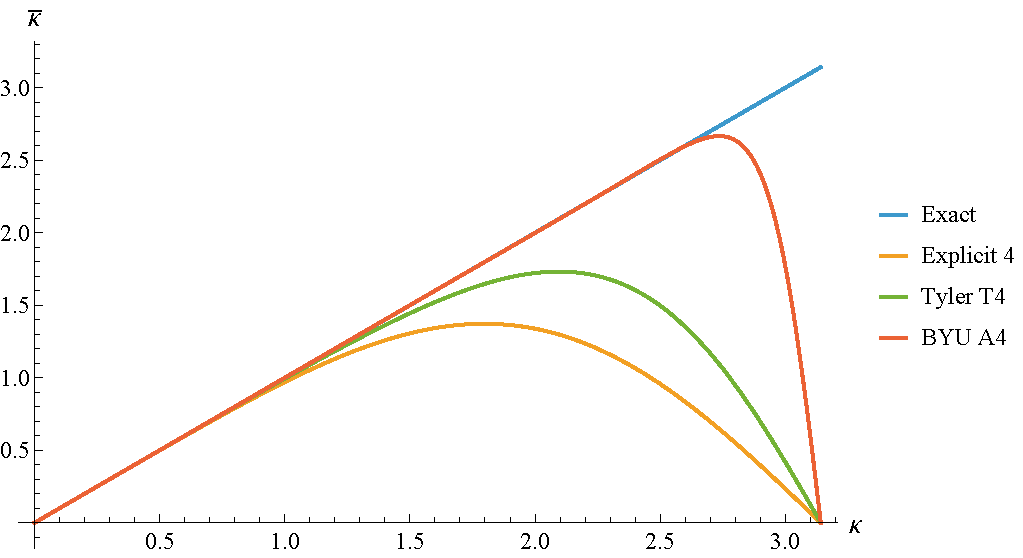
\includegraphics[width=\linewidth]{figures/1st_4th_Order_Spectral_Functions.pdf}
  \vspace{-.75cm}
  \caption{
   Comparison of spectral functions for several 4th order schemes: the explicit 4th order finite difference, a tridiagonal 4th order compact finite difference [ref Tyler], and a spectrally-optimized pentadiagonal 4th order compact finite difference [this work].
}
  \label{fig:4th_spectral_functions}
\end{figure}

We construct the following error quantity from the spectral function~\cite{yo}, namely 
\begin{equation}
E(\alpha_i, a_i) = \int_{0}^{r \pi}{\bigl[ \bar{\kappa} - \kappa \bigr]^2 D(\kappa)^2 \, d\kappa}
\end{equation}
where $D(\kappa)$ is simply the denominator in the spectral function, Eq. (\ref{spectral_function}). In general, an arbitrary weighting function can be used, but this form is chosen so that the integral can be computed analytically [ref Zhou Zhang 2011]. The parameter $r \in (0,1]$ in the upper bound of the integral is referred to as the ``fractional cutoff wavenumber,'' and represents the maximum modified wavenumber $\kappa$ over which the spectral error is optimized. It has been suggested [ref Chen 2023] to have a lower cutoff wavenumber around $0.5$ or $0.75$ to avoid over-optimization on higher-wavenumber modes, while others [ref Kim 2007] have used higher cutoff wavenumbers such as $0.839$. In this work, we develop several families of CFD operators for several values of the cutoff wavenumber from $0.6$ to $0.85$.

We minimize the error $E$ by substituting the solutions of the Taylor constraint equations up to a given order of accuracy for our ``fixed parameters'' and by imposing constraints of the form
\begin{equation}
\frac{\partial E}{\partial a_i} = 0,
\end{equation} 
for our ``free parameters.'' As the error quantity is quadratic with respect to its arguments, the resulting constraint equations form a linear system with respect to these free parameters, and hence yield a unique solution for a spectrally-optimized CFD scheme.

\subsubsection{Boundary Scheme}
If we wish to maintain the banded-diagonal form of these CFD operators on the boundary, we must develop a boundary closure using shifted stencils. However, it has been shown [refs] that centered stencils provide greater benefits in terms of accuracy and stability. Following the approach of Wu et al. [ref Kim 2024], we use a polynomial to extrapolate our function to grid points which lie beyond the boundary of our numerical domain.

If we have interior coefficients $\alpha_1$ through $\alpha_m$ on the LHS and $a_1$ through $a_k$ on the RHS, then the order of the extrapolation polynomial must be at least $\ell = 3k+m+1$.  
%$$
%P_{order} = 3k + m + 1.
%$$
We increase the order of this polynomial by one in order to introduce an extra free parameter in order to optimize the spectral behavior at and near the boundary. Following [ref Kim 2024], we construct the extrapolation polynomial, 
\begin{equation}
P(\hat{x}) = \sum_{s=0}^{\ell} p_s {\hat x}^s, 
\end{equation}
where ${\hat x} \equiv (x_j - x_0)/h$ and we use the information from the function and its derivatives: 
$$
\begin{cases}
    P(j) = f_j, \quad j = 0, 1, \dots, 2k\\
    \frac{dP}{dx}(j) = f'_j, \quad j = 0, 1, \dots, k + m\\
    \frac{d^n P}{dx^n}(\hat{y}) = 0.
\end{cases}
$$
The parameter $\hat{y}$ is a value which will be used for optimizing the boundary closures later on. The quantity $n$ is an arbitrary integer which should be at least greater than or equal to the order of accuracy of the scheme and at most less than or equal to the order of the extrapolation polynomial. We have found that a lower value of $n$ leads to a larger family of minima in our boundary error quantity and thus a larger family of error-optimized boundary closures.

Once we have solved the system above to find the coefficients of the extrapolation polynomial, we construct a centered stencil for each of the boundary nodes, substituting in the extrapolation polynomial at each of the grid points which lie beyond the domain. Finally, we can rearrange the resulting equations into the shifted stencils which can be implemented, and the shifted stencil boundary coefficients can be read off in terms of the free parameter $\hat{y}$ only.

As with the approach to optimizing the interior scheme, we Fourier transform the shifted boundary stencils to define a spectral function. For the $m$th boundary node, we find:
\begin{align*}
\bar{\kappa}_m(\kappa) &= \frac{1}{A_m(\kappa)^2 + B_m(\kappa)^2} \big[ A_m(\kappa) D_m(\kappa) - B_m(\kappa) C_m(\kappa)\\
&  \qquad\qquad\qquad - i (A_m(\kappa) C_m(\kappa) + B_m(\kappa) D_m(\kappa)) \big],
\end{align*}
where:
\begin{align*}
    A_m(\kappa) &= \sum_{j=0}^{3}{\gamma_{mj} \cos{(j \kappa)}}, \quad B_m(\kappa) = \sum_{j=0}^{3}{\gamma_{mj} \sin{(j \kappa)}},\\
    C_m(\kappa) &= \sum_{j=0}^{6}{a_{mj} \cos{(j \kappa)}}, \quad D_m(\kappa) = \sum_{j=0}^{6}{a_{mj} \sin{(j \kappa)}}.
\end{align*}
%\nate{TODO: Need to generalize the upper bounds of the sums, and also explain what $a_{mj}$ and $\gamma_{mj}$ are (the bd coefficients). In general I think I need to be a bit more clear in this section about the indices being used, maybe define some things like $n_L$ and $n_R$ at the beginning.}

Note that because the boundary stencils are shifted, their spectral functions have real and imaginary components, corresponding to both dispersive and dissipative behavior in the numerical scheme.

At this point, many different error quantities could be constructed in order to optimize specific features of the boundary closure. For example, an error quantity could be chosen to optimize only on the imaginary part of the spectral function in order to minimize unwanted dissipative modes. In the present work, we use the error quantity
$$
E_m = \int_{0}^{r \pi}{\Big[ \big| \Re(N_m(\kappa)) + i \Im(N_m(\kappa)) \big| - \kappa D_m(\kappa) \Big]^2 \ d\kappa}
$$
where $N_m(\kappa)$ and $D_m(\kappa)$ represent the numerator and denominator of the spectral function $\bar{\kappa}_m(\kappa)$, respectively; i.e., we have set:
\begin{align*}
    \Re(N_m(\kappa)) &= A(\kappa) D(\kappa) - B(\kappa) C(\kappa),\\
    \Im(N_m(\kappa)) &= -A(\kappa) C(\kappa) - B(\kappa) D(\kappa),\\
    D_m(\kappa) &= A(\kappa)^2 + B(\kappa)^2.
\end{align*}
Note that each boundary node has a spectral function and thus error quantity which is independent from each other. As each of the boundary coefficients $a_{mj}$ and $\gamma_{mj}$ only depend on the free parameter $\hat{y}$, then each error quantity also only depends on $\hat{y}$. Since the error functions are decoupled, we opt to use a separate free parameter $\hat{y}_m$ for each boundary node. Clearly, even with a similar weighting function to the interior scheme, this error integral is not analytically integrable, so we must numerically integrate the error quantity over a grid of possible values for $\hat{y}_m$. [ref Kim 2024] suggests testing $\hat{y}_m \in (-6,6)$, but we have found that the minima in the error are typically found for $\hat{y}_m \in (-1,5)$.

Since each boundary error function $E_m(\hat{y}_m)$ has several minima, we obtain a family of spectrally-optimized boundary closures by taking all possible combinations of optimal $\hat{y}_m$ values.

%\nate{Do we need a section talking about stability?}



%\subsection{Fourth-order operators}



% \subsection{EM4 Convergence}
% \begin{table}[p]
% \centering
% \small
% \setlength{\tabcolsep}{3.5pt}
% \renewcommand{\arraystretch}{1.15}
% \resizebox{\textwidth}{!}{%
% \begin{tabular}{lccccccc}
% \toprule
% Variable & A4\_3 & A6\_2 & C4\_1 & C6\_4 & E4 & E6 & E8 \\
% \textbf{Avg over vars} & \textbf{5.158} (6) & \textbf{6.618} (6) & \textbf{4.436} (6) & \textbf{5.788} (6) & \textbf{3.916} (6) & \textbf{5.799} (6) & \textbf{6.883} (6) \\
% \midrule
% U\_B0 & 5.088 $\pm$ 0.364 (7) & 6.473 $\pm$ 0.272 (7) & 4.460 $\pm$ 0.178 (7) & 6.075 $\pm$ 0.280 (7) & 3.918 $\pm$ 0.028 (7) & 5.783 $\pm$ 0.073 (7) & 6.574 $\pm$ 0.098 (7) \\
% U\_B1 & 5.079 $\pm$ 0.391 (7) & 6.472 $\pm$ 0.281 (7) & 4.367 $\pm$ 0.176 (7) & 6.228 $\pm$ 0.225 (7) & 3.918 $\pm$ 0.028 (7) & 5.783 $\pm$ 0.073 (7) & 6.574 $\pm$ 0.098 (7) \\
% U\_B2 & 5.166 $\pm$ 0.674 (7) & 6.639 $\pm$ 0.314 (7) & 4.241 $\pm$ 0.194 (7) & 6.613 $\pm$ 0.286 (7) & 3.899 $\pm$ 0.058 (7) & 5.779 $\pm$ 0.115 (7) & 6.743 $\pm$ 0.104 (7) \\
% U\_E0 & 5.390 $\pm$ 0.344 (7) & 6.693 $\pm$ 0.470 (7) & 4.259 $\pm$ 0.123 (7) & 6.548 $\pm$ 0.232 (7) & 3.908 $\pm$ 0.038 (7) & 5.790 $\pm$ 0.084 (7) & 6.822 $\pm$ 0.196 (7) \\
% U\_E1 & 5.373 $\pm$ 0.346 (7) & 6.679 $\pm$ 0.450 (7) & 4.269 $\pm$ 0.122 (7) & 6.512 $\pm$ 0.257 (7) & 3.908 $\pm$ 0.038 (7) & 5.790 $\pm$ 0.084 (7) & 6.822 $\pm$ 0.196 (7) \\
% U\_E2 & 4.853 $\pm$ 0.284 (7) & 6.751 $\pm$ 0.292 (7) & 5.018 $\pm$ 0.165 (7) & 2.754 $\pm$ 0.894 (7) & 3.946 $\pm$ 0.012 (7) & 5.869 $\pm$ 0.017 (7) & 7.767 $\pm$ 0.028 (7) \\
% \bottomrule
% \end{tabular}%
% }
% \caption{A\_05: Evolved variables (cells show mean ± std (N); avg row shows weighted mean over variables, with (\#vars))}
% \end{table}
% \begin{figure}\centering
%   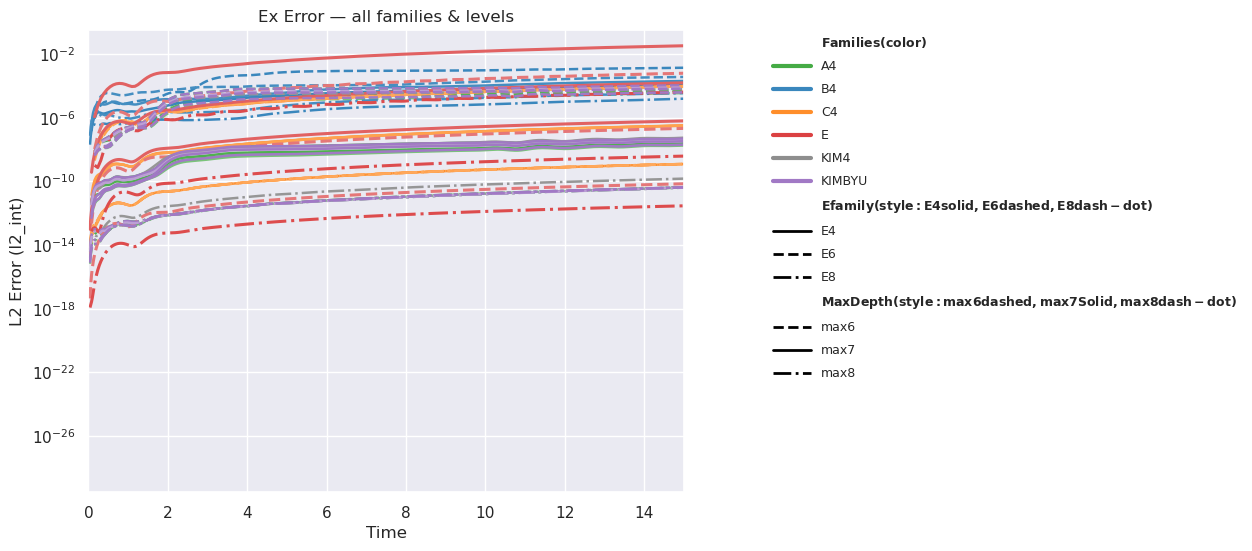
\includegraphics[width=\linewidth]{figures/U_E0_DIFF__ALL_FAMILIES.png}  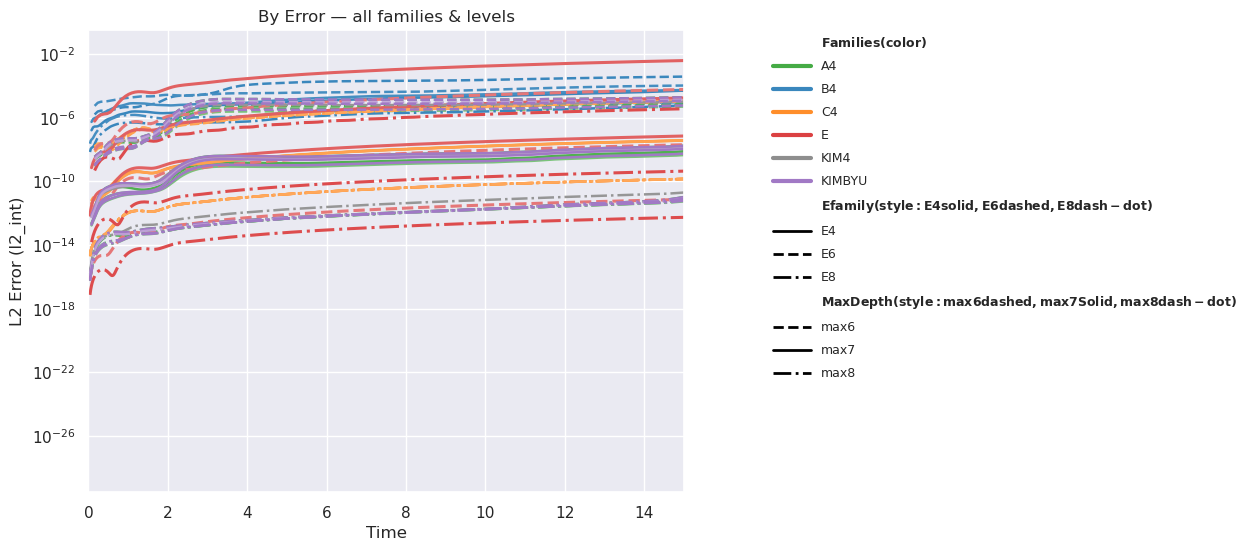
\includegraphics[width=\linewidth]{figures/U_B1_DIFF__ALL_FAMILIES.png}
%   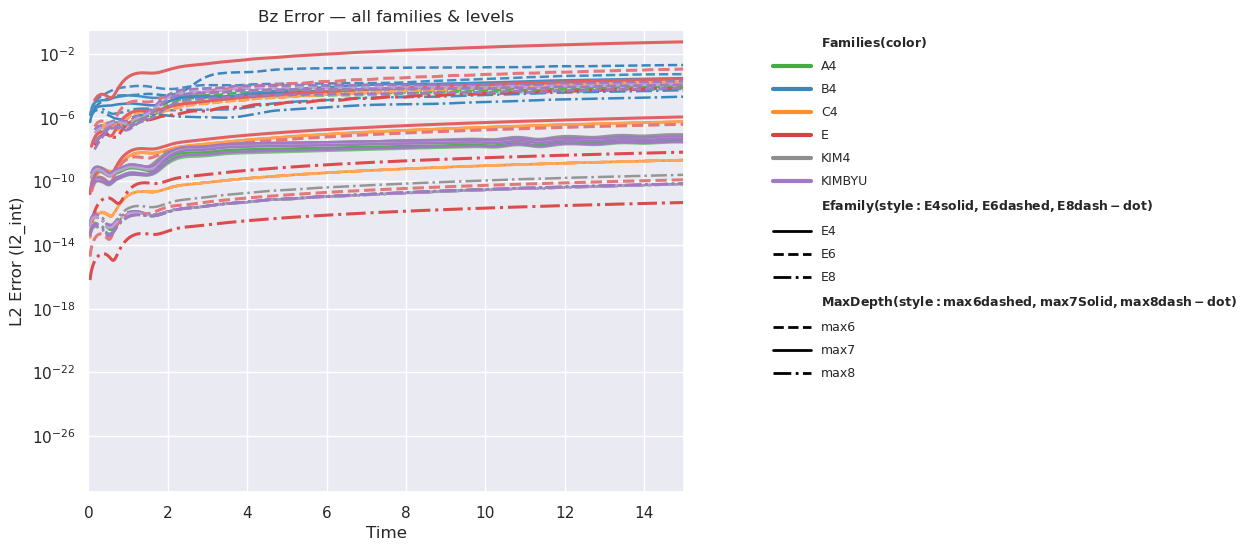
\includegraphics[width=\linewidth]{figures/U_B2_DIFF__ALL_FAMILIES.png}
%   \vspace{-.75cm}
%   \caption{
%     Comparison of error in the magnetic field component, $B_y$, for different CFD and explicit schemes.   component  for $q=4$. 
%     % describe sub-plots
%     We see .  blah blah blah
%   }
%   \label{fig:B_y_allfams}
% \end{figure}


\section*{Symbolic Matrices}
This is specifically the formulation of the 1A family of matrices.

\[
\mathbf{P} = 
\left(
\begin{array}{ccccccccccc}
1 & \gamma_{01} & \gamma_{02} & 0 & 0 & 0 & 0 & 0 & \cdots & 0 \\
\gamma_{10} & 1 & \gamma_{12} & \gamma_{13} & 0 & 0 & 0 & 0 & \cdots & 0 \\
\gamma_{20} & \gamma_{21} & 1 & \gamma_{23} & \gamma_{24} & 0 & 0 & 0 & \cdots & 0 \\
0 & \beta & \alpha & 1 & \alpha & \beta & 0 & 0 & \cdots & 0 \\
\vdots & \ddots & \ddots & \ddots & \ddots & \ddots & \ddots & \ddots & \ddots & \vdots \\
0 & \cdots & 0 & 0 & \beta & \alpha & 1 & \alpha & \beta & 0 \\
0 & \cdots & 0 & 0 & 0 & \gamma_{24} & \gamma_{23} & 1 & \gamma_{12} & 0 \\
0 & \cdots & 0 & 0 & 0 & 0 & \gamma_{13} & \gamma_{12} & 1 & \gamma_{10} \\
0 & \cdots & 0 & 0 & 0 & 0 & 0 & \gamma_{02} & \gamma_{01} & 1 \\
\end{array}
\right)
\]

\[
\mathbf{Q} = 
\left(
\begin{array}{ccccccccccc}
a_{00} & a_{01} & a_{02} & a_{03} & a_{04} & a_{05} & a_{06} & 0 & \cdots & 0 \\
a_{10} & a_{11} & a_{12} & a_{13} & a_{14} & a_{15} & a_{16} & 0 & \cdots & 0 \\
a_{20} & a_{21} & a_{22} & a_{23} & a_{24} & a_{25} & a_{26} & 0 & \cdots & 0 \\
-a_3 & -a_2 & -a_1 & 0 & a_1 & a_2 & a_3 & 0 & \cdots & 0 \\
\vdots & \ddots & \ddots & \ddots & \ddots & \ddots & \ddots & \ddots & \ddots & \vdots \\
0 & \cdots & 0 & -a_3 & -a_2 & -a_1 & 0 & a_1 & a_2 & a_3 \\
0 & \cdots & 0 & -a_{26} & -a_{25} & -a_{24} & -a_{23} & -a_{22} & -a_{21} & -a_{20} \\
0 & \cdots & 0 & -a_{16} & -a_{15} & -a_{14} & -a_{13} & -a_{12} & -a_{11} & -a_{10} \\
0 & \cdots & 0 & -a_{06} & -a_{05} & -a_{04} & -a_{03} & -a_{02} & -a_{01} & -a_{00} \\
\end{array}
\right)
\]


% \section*{Tables of Coefficients}
% The specific coefficients in this table are for 1A4 Op 5.

% - How do I get the spacing to line up when there's negative signs? And also with the ``blank'' entries? I was trying to somewhat mimic the format of Kim 2024's coefficient tables.

% - It may be better to put the interior coefficients separately if we are listing coefficients for several A4 operators; they have the same interior but different boundary coefficients (for example, A4 Op 2 vs. A4 Op 13).

% - Is it worth noting the condition that $a_{ii} = -\sum_{k \neq i}{a_{ik}}$? Kim often omits the $a_{ii}$ entries from his coefficient tables because of this, I personally find it helpful and cleaner to have it filled in, but we have verified before that the coefficients we're getting satisfy this condition, as they should.

% \begin{table}[h!]
% \centering
% \begin{tabular}{|c|c c c|} 
%  \hline
%  Interior Nodes & Node 0 & Node 1 & Node 2 \\
%  \hline
%  $\alpha$ \quad $0.577046020129014$ & - \quad - & $\gamma_{10}$ \quad $0.081850642218291$ & $\gamma_{20}$ \quad $0.010832502509738$ \\
%  $\beta$ \quad $0.089008368450770$ & $\gamma_{01}$ \quad $9.820500862970050$ & - \quad - & $\gamma_{21}$ \quad $0.238186806866178$ \\
%  - \quad - & $\gamma_{02}$ \quad $10.282867809058310$ & $\gamma_{12}$ \quad $1.689062748171480$ & - \quad - \\
%  - \quad - & - \quad - & $\gamma_{13}$ \quad $0.496147893138870$ & $\gamma_{23}$ \quad $1.128279076992181$ \\
%  - \quad - & - \quad - & - \quad - & $\gamma_{24}$ \quad $0.288649699198454$ \\
%  \hline
%  $a_1$ \quad $0.651707844090089$ & $a_{00}$ \quad $-3.734452513805820$ & $a_{10}$ \quad $-0.318509096234275$ & $a_{20}$ \quad $-0.046786865516800$ \\
%  $a_2$ \quad $0.248158826270106$ & $a_{01}$ \quad $-10.765902315893960$ & $a_{11}$ \quad $-1.396944235854646$ & $a_{21}$ \quad $-0.510448282160808$ \\
%  $a_3$ \quad $0.006009630649828$ & $a_{02}$ \quad $11.158777481815810$ & $a_{12}$ \quad $0.536401605870469$ & $a_{22}$ \quad $-0.770033072247311$ \\
%  - \quad - & $a_{03}$ \quad $3.893279579988119$ & $a_{13}$ \quad $1.122316892895001$ & $a_{23}$ \quad $0.622893361976584$ \\
%  - \quad - & $a_{04}$ \quad $-0.638983973815703$ & $a_{14}$ \quad $0.059450604503400$ & $a_{24}$ \quad $0.672712515935698$ \\
%  - \quad - & $a_{05}$ \quad $0.095877273974209$ & $a_{15}$ \quad $-0.002743838025071$ & $a_{25}$ \quad $0.033041689527406$ \\
%  - \quad - & $a_{06}$ \quad $-0.008595531676509$ & $a_{16}$ \quad $0.000028066844770$ & $a_{26}$ \quad $-0.001379347514431$ \\
%  \hline
% \end{tabular}
% \caption{Coefficients for First Derivative A4 Operator \#5}
% \label{table:1stA4Op5coeff}
% \end{table}


%\subsection{Sixth-order operators}

\section{Test cases}

Having sketched the process of computing boundary-closed CFD operators for a given order of accuracy, we here present several tests of these operators as applied in specific systems of PDEs.  

We begin with a 1D nonlinear system, namely Burgers' equation.  We also consider Maxwell's equations in full 3D together with hyperbolic divergence cleaning.  We return to nonlinear problems with a 3D nonlinear sigma model and conclude with the Einstein equations with the evolution of Teukolsky gravitational waves. 

In each case, the basic results are similar.  Namely, the use of CFDs at some accuracy order perform better than a comparable explicit FD scheme, sometimes by more than an order of magnitude as measured by.  Effectively, the CFDs are providing comparable error profiles at half the resolution of the FDs.  


%\subsection{Classical wave equation}



\subsection{One-Dimensional Nonlinear Burgers'}

Our first test uses the nonlinear one-dimensional viscous Burgers' Equation,
\begin{equation}
\label{eq:BurgersEq}
\frac{\partial f}{\partial t}
=
-f\frac{\partial f}{\partial x}
+
\frac{\partial^2 f}{\partial x^2},
\qquad
-\infty < x < \infty,
\qquad
t \ge 0.
\end{equation}
where the solution $f(x,t)$ depends only on $x$ and $t$, and the viscosity coefficient is fixed at $1$ for simplicity.

This admits a closed form solution against which we will compare the numerical solution.  It is 
\begin{equation}
    f(x,t) = \frac{2}{1+e^{x-t}}.
\end{equation}
The initial condition, of course, is thus 
\begin{equation}
    \phi(x,t=0) = \frac{2}{1+e^x}.
\end{equation}
%This initial condition is chosen because it admits a closed-form analytical solution for comparison. The corresponding solution is

In solving this problem numerically, we approximate both first and second spatial derivatives using CFDs and explicit FDs separately.  The time integration is done using a fourth order Runge-Kutta scheme as will be true for all subsequent tests as well.   
%our tests.  This will leave the equation in a semidiscretized form, from which we may advance the solutions in time using a method-of-lines approach with a stable time-integration method.

To focus in this test problem on the interior parts of the CFDs, we take a domain of $-100 \le x \le 100$ and limit the simulation time to $0 \le t < 50$. Because the solution approaches constant states far from the transition region near $x=t$, fixed Dirichlet boundary conditions provide an accurate approximation on the truncated domain.  Appropriate boundary-closed operators continue to be use

The continuous domain $[-100,100]$ is divided into $N$ uniform cells of width $h$. Using a grid defined at the cell boundaries, we will have $N+1$ grid points to represent the domain. Defining $\phi_i(t) = \phi(-100 + ih,t)$ to be the $i$th point of the solution along the domain, with $i$ ranging from $0$ to $N$, we can write equation \ref{eq:BurgersEq} in the semidiscrete form:
\begin{equation}
    \frac{d \phi_i}{d t} = -\phi_i \textbf{D}_1 \phi_i + \textbf{D}_2\phi_i,
\end{equation}
where $\textbf{D}_1$ and $\textbf{D}_2$ denote the discrete first- and second-derivative operators, respectively

From here, the standard fourth-order Runge--Kutta (RK4) method is implemented to advance our solution in time. At each time step, including the intermediary stages in the integration, the Dirichlet boundary conditions are imposed on the first and last entries of the solution. This process is repeated for select resolutions of $N$, $2N$, and $4N$, and the $L_2$-norm of the error when compared with the analytic solution is calculated.

Figures \ref{fig:4th_burgers_error} and \ref{fig:6th_burgers_error} both show the analytic error of these evolutions using 4 different operators at three different resolutions. The values chosen are $N=200,400,800$ for the low, medium, and high resolutions respectively. The E4 and E6 operators are both standard explicit finite difference schemes with 4th- and 6th-order accuracy for both first and second derivatives. The A4 and C4 operators are two of the optimized compacts schemes at 4th order for the first derivative, with the choice of a non-optimized compact tridiagonal scheme for the second derivative. Likewise, the C6 operator is another optimized 6th order compact scheme for the first derivative in tandem with a non-optimized tridiagonal compact scheme in the second derivative. In both cases, the compact schemes at low resolutions perform almost as well or better than the explicit schemes at a resolution with twice as many points. This shows a definite improvement in accuracy with the compact schemes.

\begin{figure}\centering
  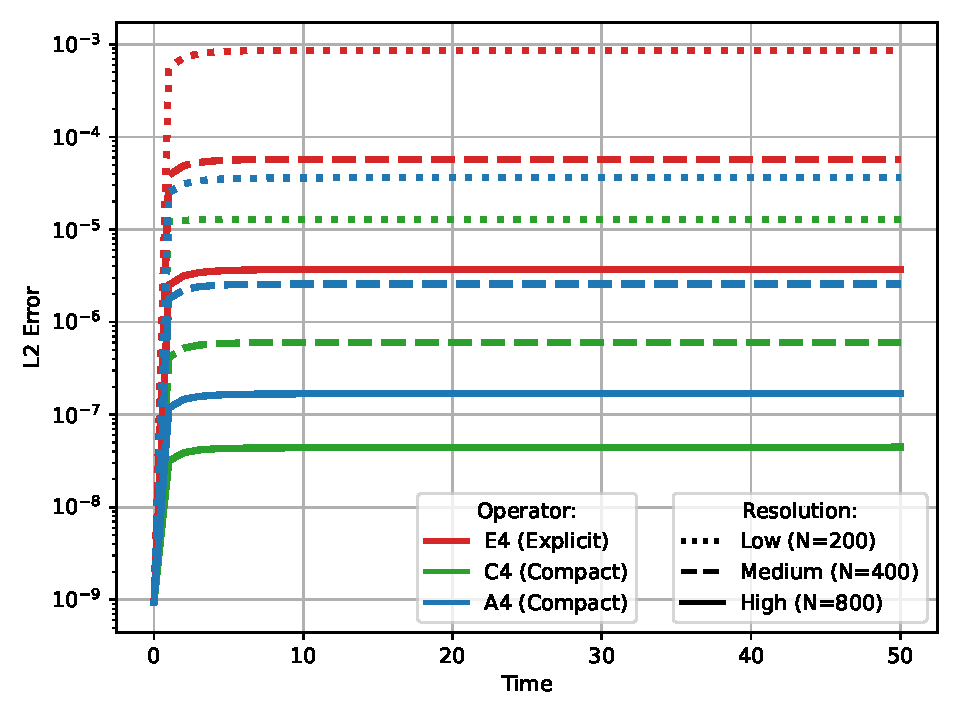
\includegraphics[width=\linewidth]{figures/4th_order_Burgers.pdf}
  %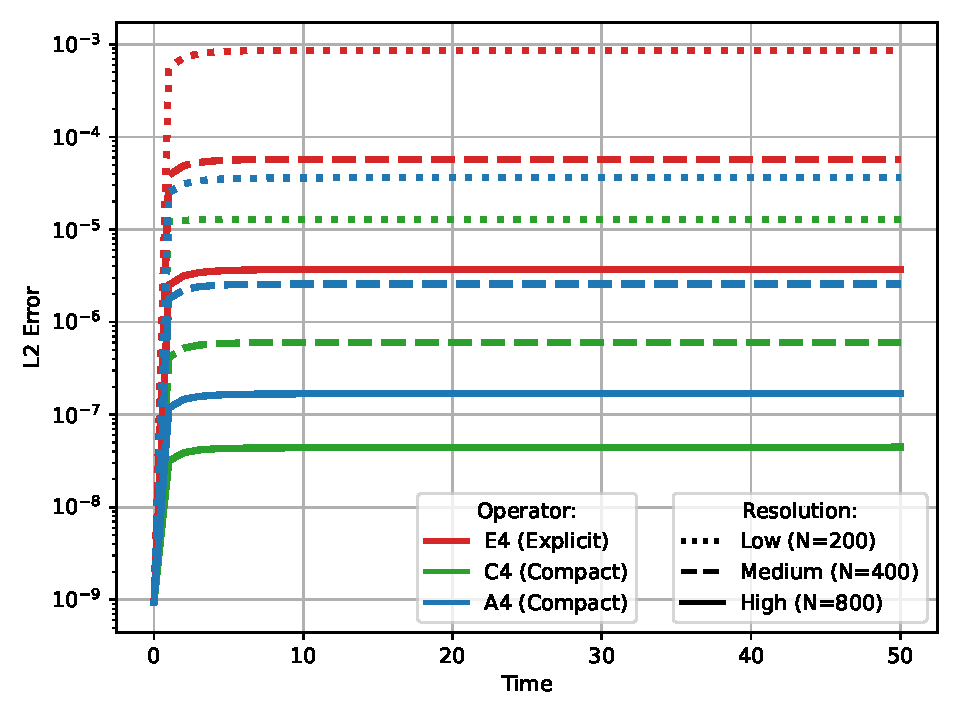
\includegraphics[width=\linewidth]{figures/4th_order_Burgers.pdf}
  \vspace{-.75cm}
  \caption{
   Analytic error of Burger's equation at different resolutions with 4th order operators
}
  \label{fig:4th_burgers_error}
\end{figure}

\begin{figure}\centering
  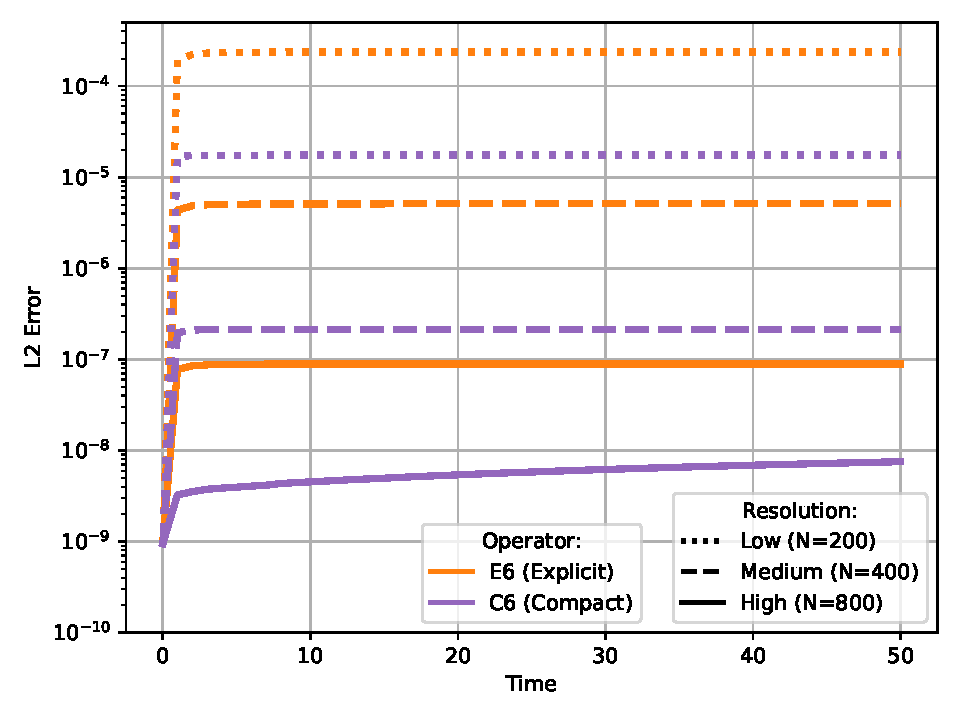
\includegraphics[width=\linewidth]{figures/6th_order_Burgers.pdf}
  %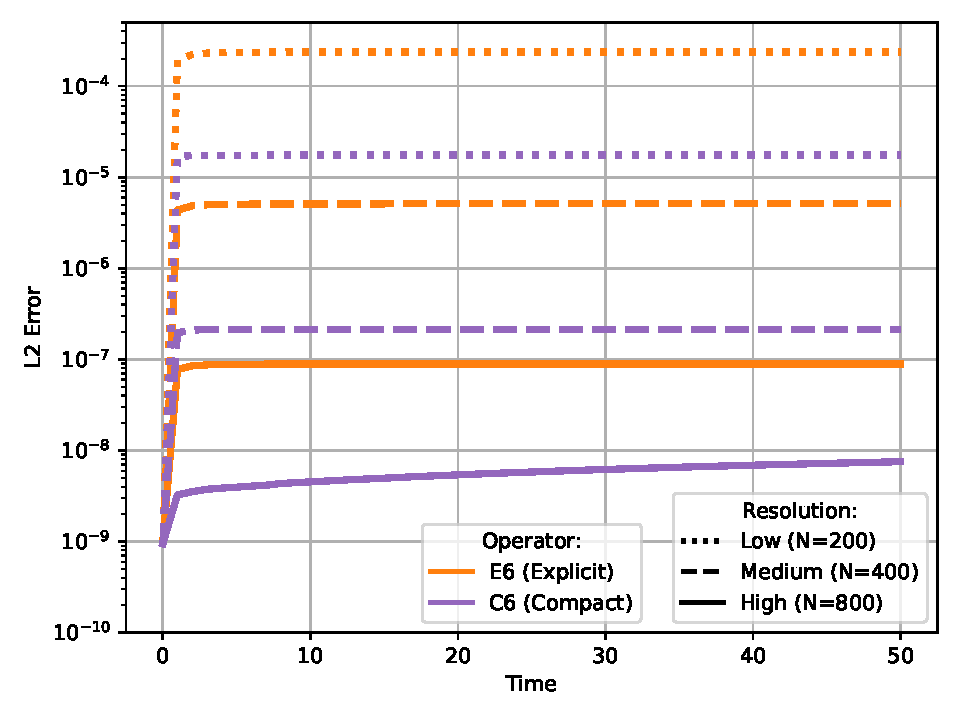
\includegraphics[width=\linewidth]{figures/6th_order_Burgers.pdf}
  \vspace{-.75cm}
  \caption{
   Analytic error of Burger's equation at different resolutions with 6th order operators
}
  \label{fig:6th_burgers_error}
\end{figure}


\subsection{Maxwell equations}
\label{sec:maxwell_equations}

The Maxwell equations provide a useful physical system for testing and
comparing different computational methods. They form a linear system with
known solutions, while retaining sufficient structure to make the numerical
tests nontrivial. For example, the Maxwell equations contain hyperbolic
evolution equations for the electric and magnetic fields, $\mathbf{E}$ and
$\mathbf{B}$, respectively,
\begin{equation}
\label{eq:maxwell_evolution}
\frac{\partial \mathbf{E}}{\partial t}
    = \nabla \times \mathbf{B},
\qquad
\frac{\partial \mathbf{B}}{\partial t}
    = -\nabla \times \mathbf{E},
\end{equation}
as well as constraint equations that must hold at all times,
\begin{equation}
\label{eq:maxwell_constraints}
\nabla \cdot \mathbf{E} = 0,
\qquad
\nabla \cdot \mathbf{B} = 0.
\end{equation}
Moreover, these equations can be written in different formulations that
mimic properties of more complicated systems. For example, Knapp
et al.~\cite{Knapp:2002fm} considered a formulation intended to reproduce
features encountered when solving the Einstein field equations in numerical
relativity.

In this work, we consider the standard Maxwell system with additional
constraint damping fields, $\Psi$ and $\Phi$, which are used to damp
violations of the electric and magnetic constraints:
\begin{align}
\partial_t E_i
    &= \epsilon_{ijk}\nabla^j B^k - 4\pi J_i - \partial_i \Psi,
\label{eq:maxwell_evolution_E}
\\
\partial_t B_i
    &= -\epsilon_{ijk}\nabla^j E^k + \partial_i \Phi,
\label{eq:maxwell_evolution_B}
\\
\partial_t \Psi
    &= 4\pi \rho_e - \partial_i E^i - \kappa_1 \Psi,
\label{eq:maxwell_evolution_Psi}
\\
\partial_t \Phi
    &= \partial_i B^i - \kappa_2 \Phi,
\label{eq:maxwell_evolution_Phi}
\\
0
    &= \nabla_i E^i - 4\pi \rho_e,
\label{eq:maxwell_constraint_E}
\\
0
    &= \nabla_i B^i.
\label{eq:maxwell_constraint_B}
\end{align}

% We also consider a formulation analogous to the BSSN formulation of general relativity:
%
% \begin{align}
% \partial_t E_i
%     &= -\nabla^j \nabla_j A_i + \nabla_i \Gamma - 4\pi J_i,
% \\
% \partial_t A_i
%     &= -E_i - \nabla_i \psi,
% \\
% \partial_t \Gamma
%     &= -4\pi \rho_e - \nabla_i \nabla^i \psi,
% \\
% \partial_t \psi
%     &= -\nabla_i A^i,
% \\
% 0
%     &= \nabla_i E^i - 4\pi \rho_e,
% \\
% 0
%     &= \nabla_i A^i - \Gamma.
% \end{align}
%
% This system also includes constraint damping, with $\Gamma$ allowing for
% the elimination of mixed derivatives.

As a test case, we use a dipolar solution of Maxwell's equations. In
particular, we choose initial data from the exact solution given by Knapp
et al.~\cite{Knapp:2002fm}:
\begin{equation}
\label{eq:maxwell_dipole_potential}
A^{\hat{\phi}}
=
\mathcal{A}\sin\theta
\left[
\frac{e^{-\lambda v^2}-e^{-\lambda u^2}}{r^2}
-
2\lambda
\frac{v e^{-\lambda v^2}+u e^{-\lambda u^2}}{r}
\right].
\end{equation}
The corresponding electric field is
\begin{equation}
\label{eq:maxwell_dipole_electric_field}
\begin{aligned}
E^{\hat{\phi}}
&=
2\lambda\mathcal{A}\sin\theta
\biggl[
\frac{
    v e^{-\lambda v^2}
    -
    u e^{-\lambda u^2}
}{r^2}
\\
&\qquad\qquad
+
\frac{1}{r}
\bigl[
    (1-2\lambda v^2)e^{-\lambda v^2}
    +
    (1-2\lambda u^2)e^{-\lambda u^2}
\bigr]
\biggr].
\end{aligned}
\end{equation}
Here
\begin{equation}
u = t-r,
\qquad
v = t+r,
\end{equation}
are the retarded and advanced time coordinates, respectively.
The parameter $\mathcal{A}$ sets the initial amplitude, while $\lambda$
controls the width of the pulse. The corresponding Cartesian components are
obtained using the standard coordinate transformation from spherical to
Cartesian coordinates.

The advantage of these initial data is that they admit an analytic solution.
In our experiments, we set $\mathcal{A}=1.0$ and $\lambda=0.5$. By comparing
the evolved solution against the analytic solution, we obtain a direct
measure of the error associated with each finite difference operator. A
representative evolution is shown in Fig.~\ref{fig:em4_e0_panel}.

\begin{figure}[t]
    \centering
    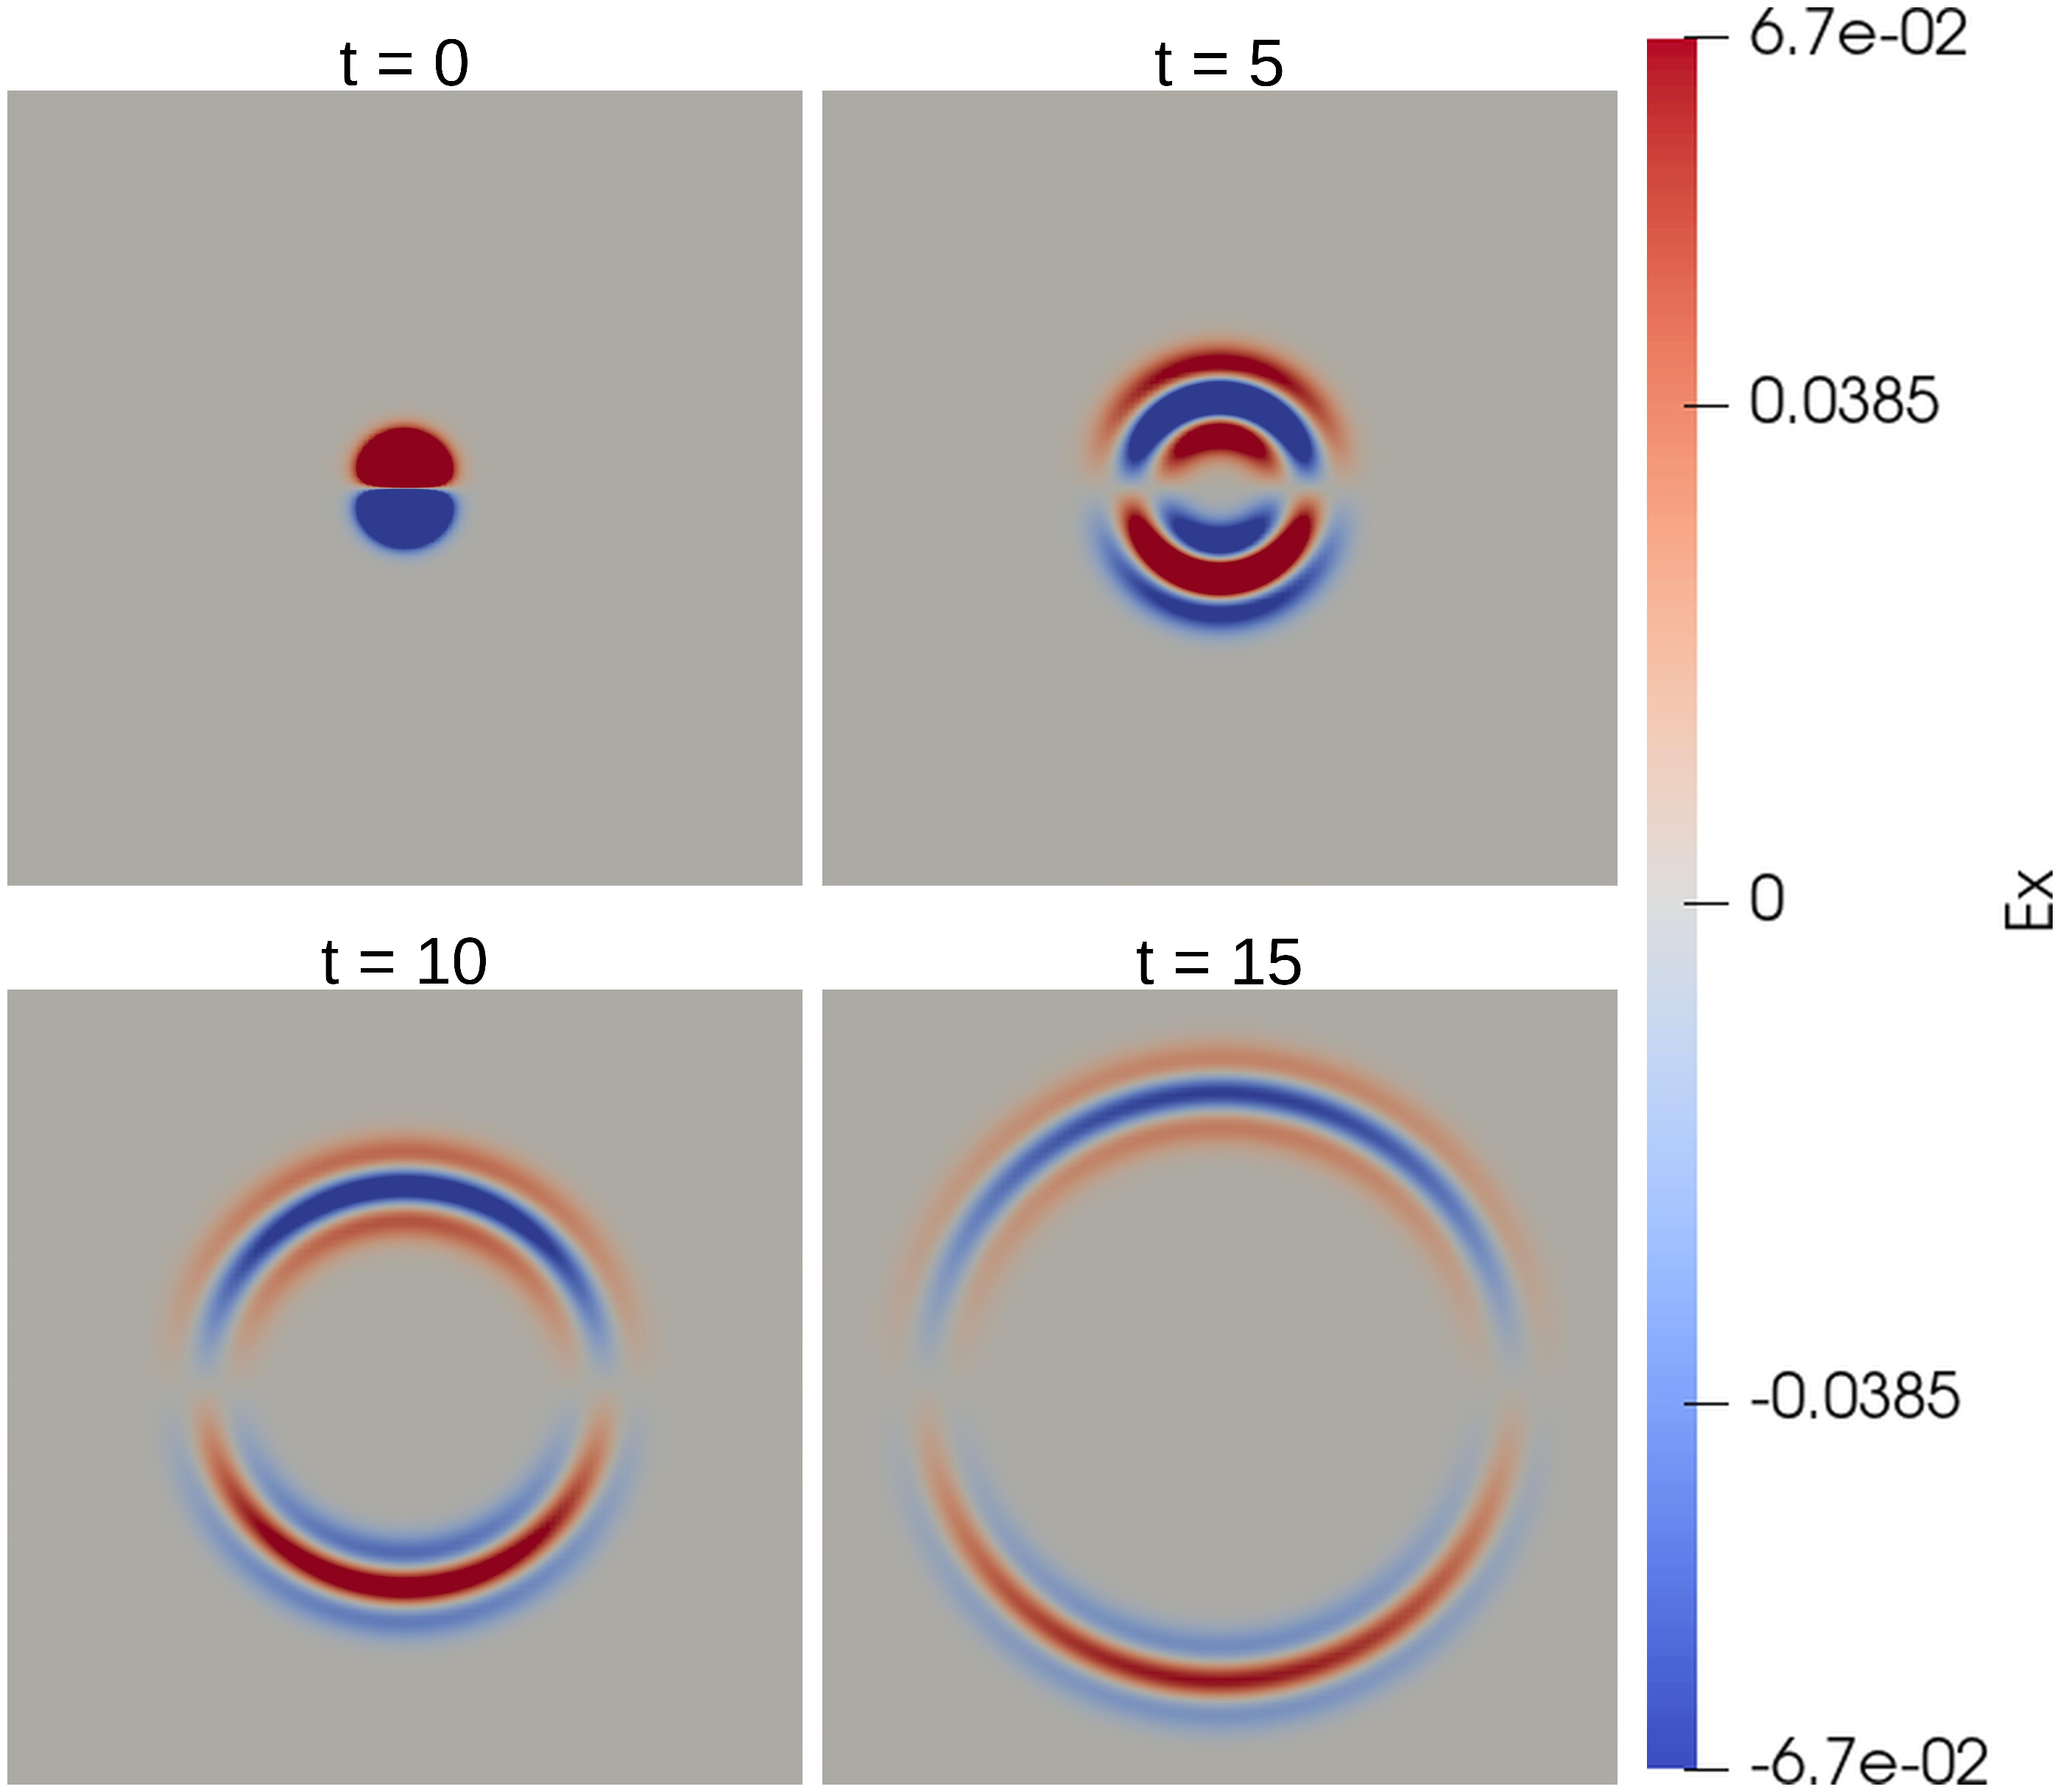
\includegraphics[width=\columnwidth]{figures/E0_panel.pdf}
    \caption{
    Evolution of the electric field component $E_x$ for the dipolar Maxwell
    test problem. The panels show representative snapshots during the
    evolution, with a shared color scale shown on the right. The initial
    dipolar pulse gradually propagates outward.
    }
    \label{fig:em4_e0_panel}
\end{figure}

\paragraph{Fourth Order Operators}

\begin{figure}[t]
    \centering
    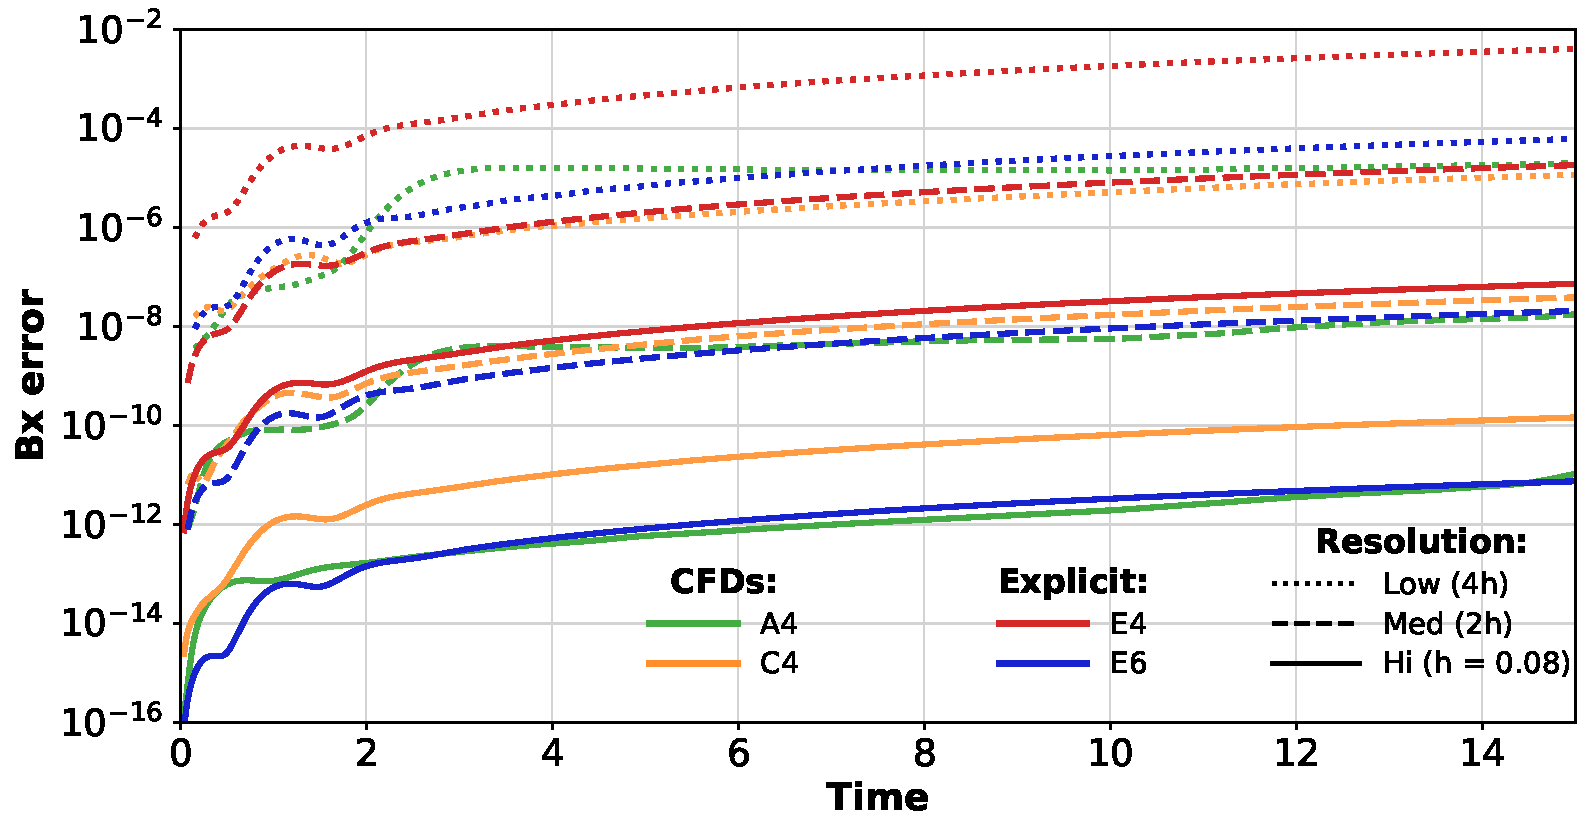
\includegraphics[width=\linewidth]{figures/U_B0_DIFF__ALL_FAMILIES.pdf}
    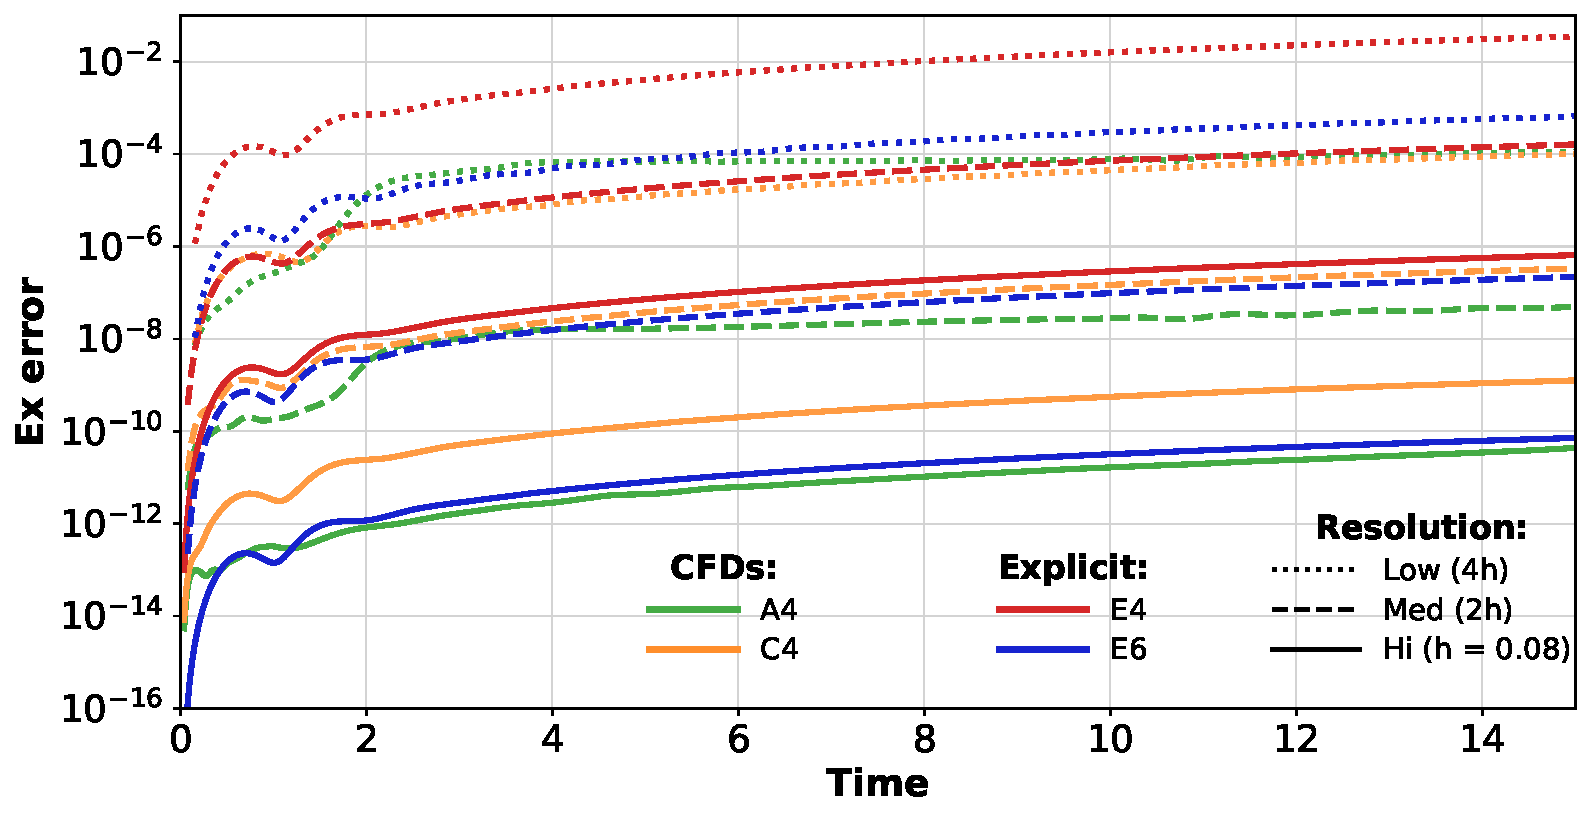
\includegraphics[width=\linewidth]{figures/U_E0_DIFF__ALL_FAMILIES.pdf}
    %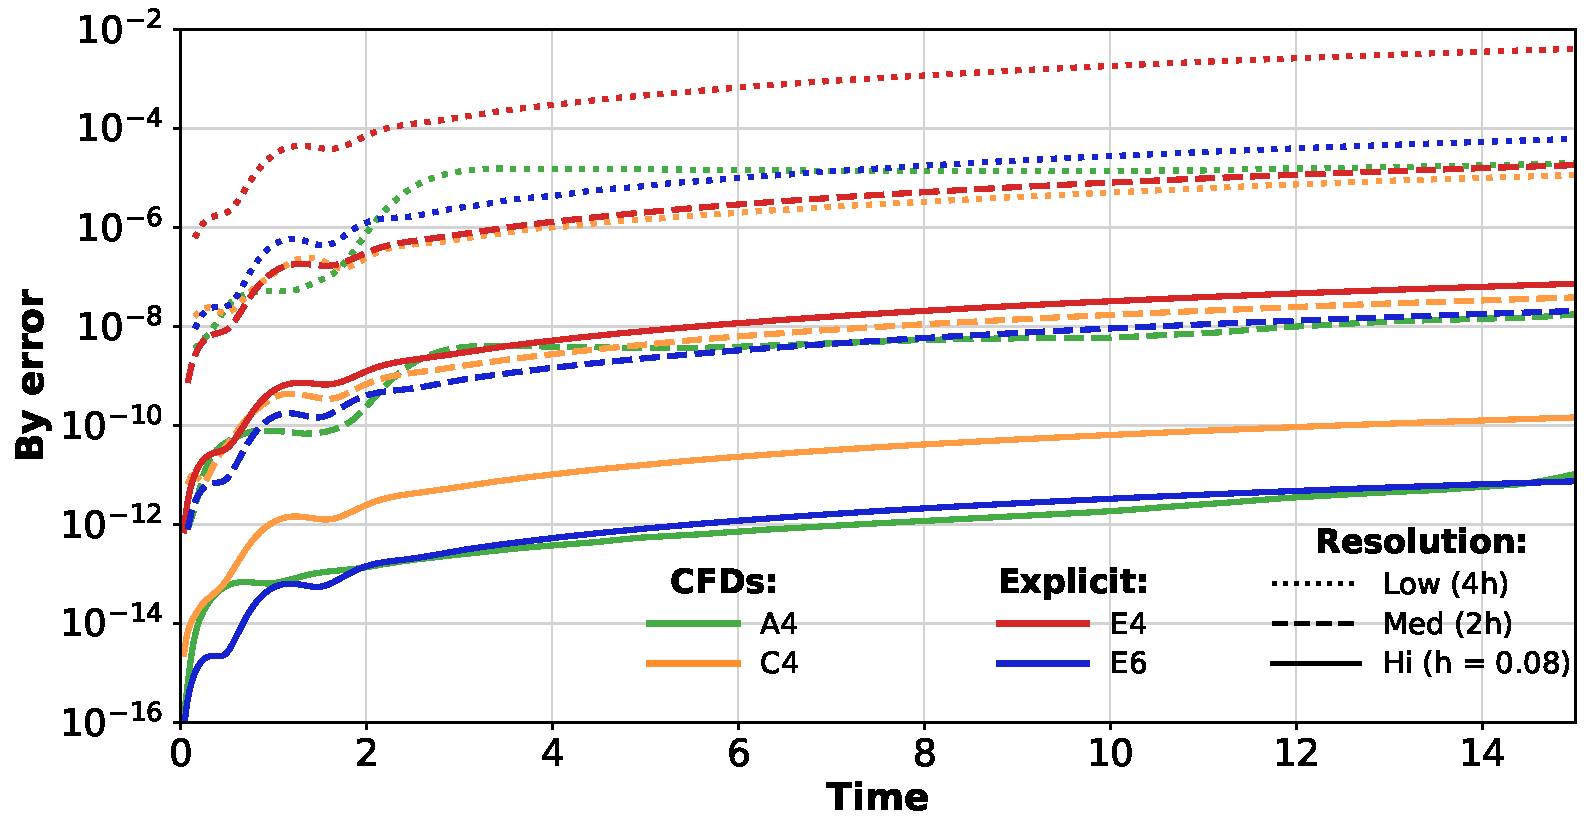
\includegraphics[width=\linewidth]{figures/U_B1_DIFF__ALL_FAMILIES.pdf}
    %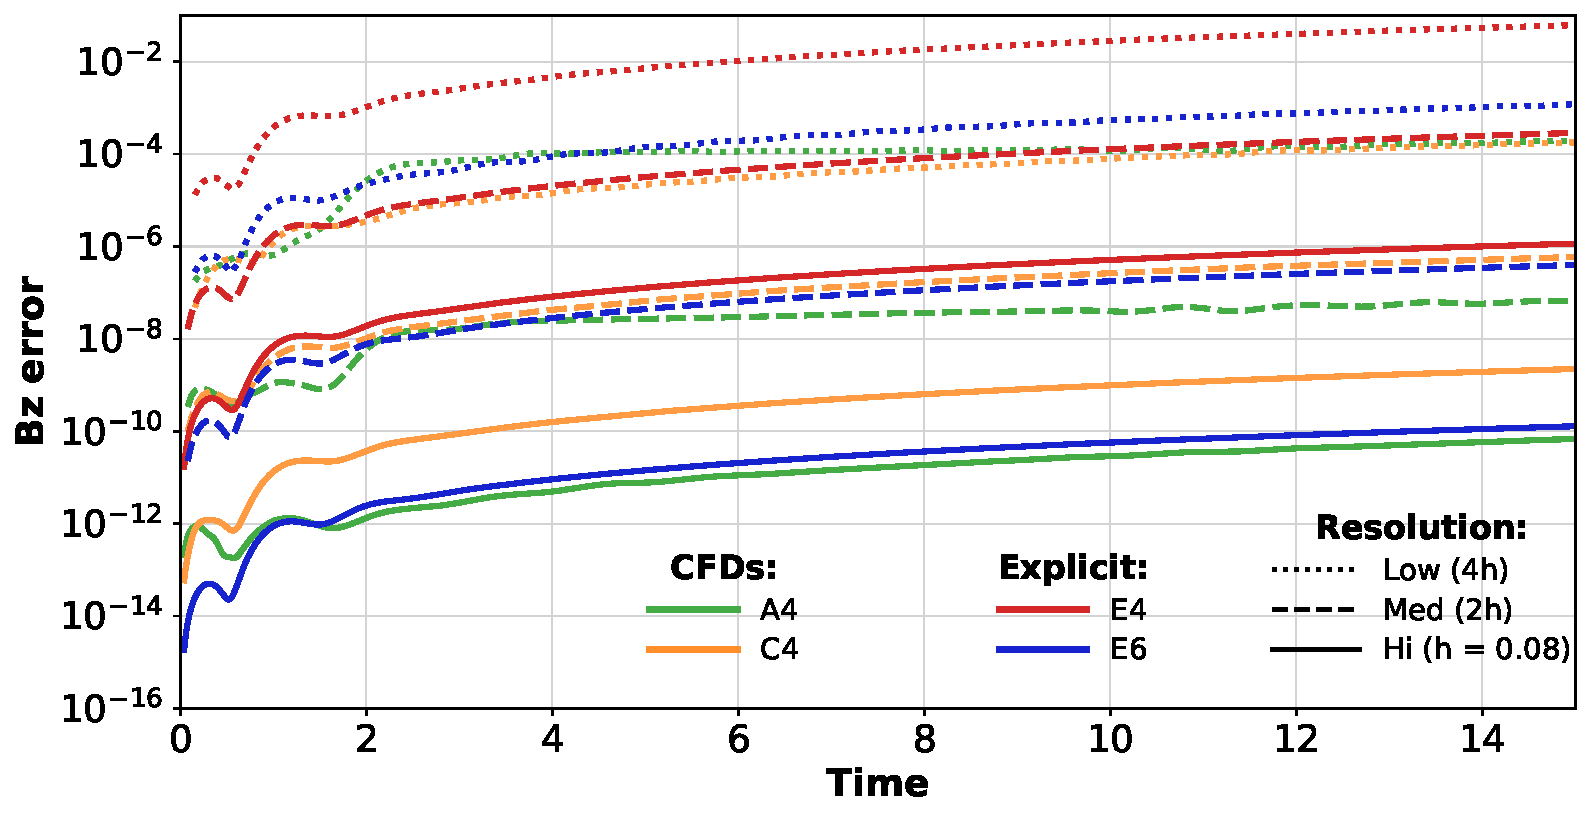
\includegraphics[width=\linewidth]{figures/U_B2_DIFF__ALL_FAMILIES.pdf}
    %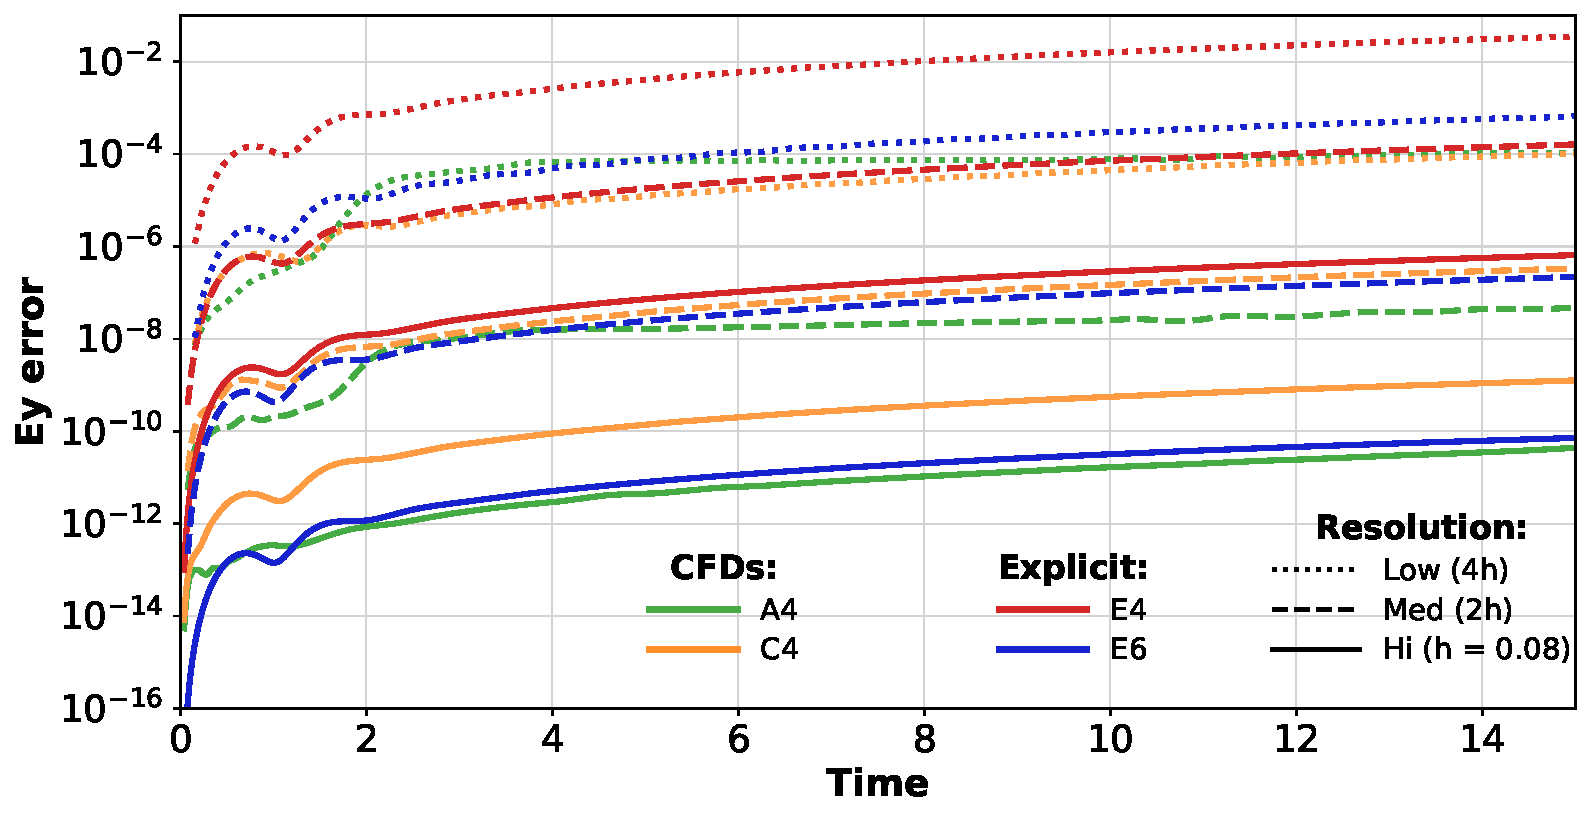
\includegraphics[width=\linewidth]{figures/U_E1_DIFF__ALL_FAMILIES.pdf}
    %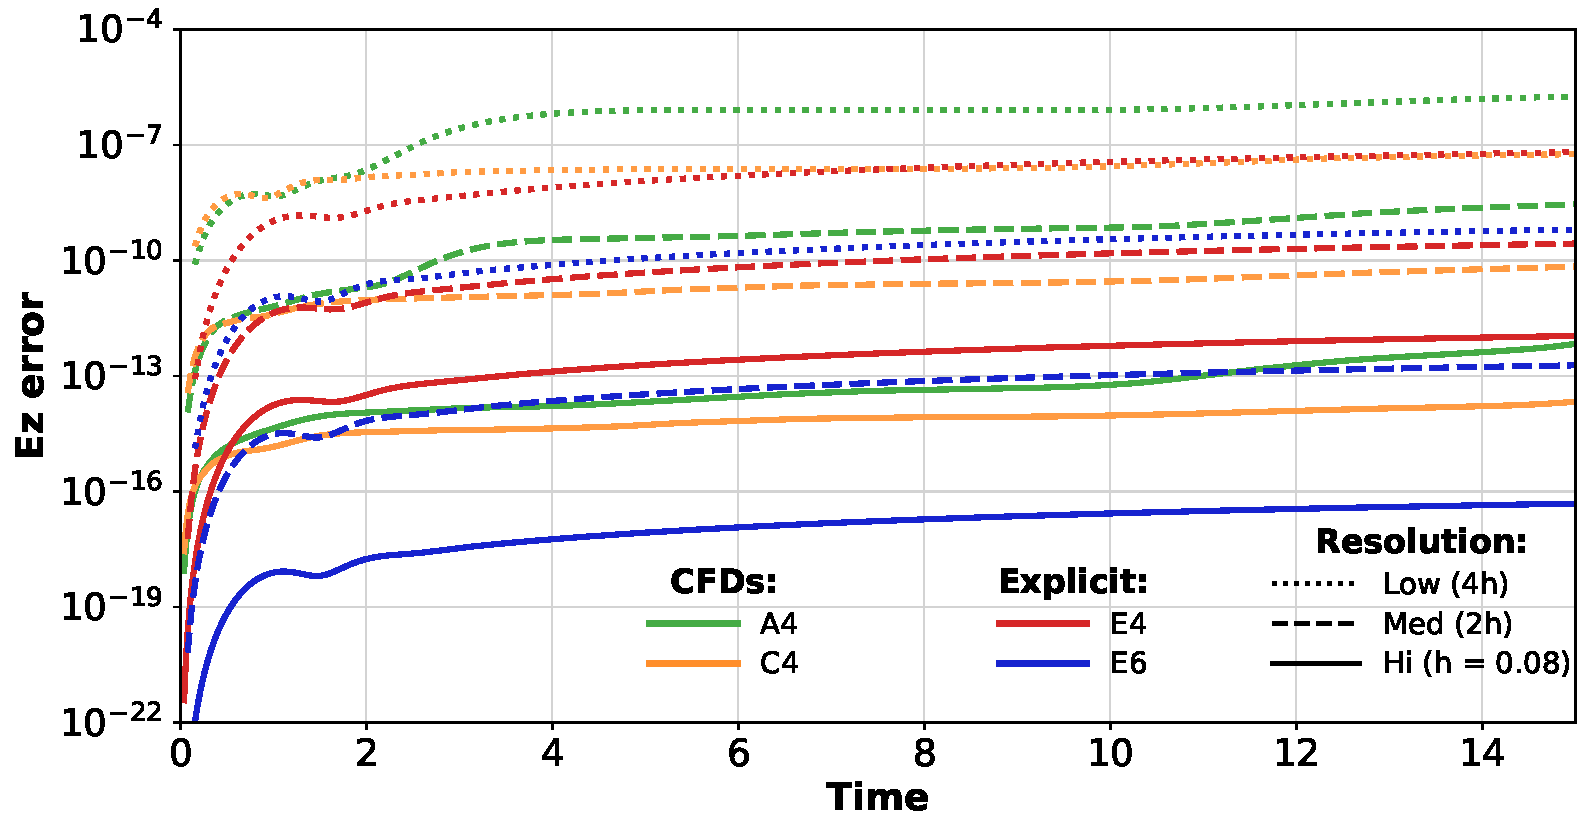
\includegraphics[width=\linewidth]{figures/U_E2_DIFF__ALL_FAMILIES.pdf}
    \vspace{-.75cm}
    \caption{
    Comparison of the errors in the magnetic and electric field components,
    $B_x$ and $E_x$, for different fourth order compact and explicit finite
    difference schemes. We plot the $L_2$ error of the numerical solution
    across the grid relative to the analytic solution. Dotted lines denote
    the low resolution runs, dashed lines denote the medium resolution runs,
    and solid lines denote the high resolution runs. The grid spacing is
    halved between each successive resolution. The fourth order compact
    operators perform comparably to their explicit counterparts at half the
    resolution and achieve error levels comparable to those of the sixth
    order explicit operators. This behavior is observed for both the A4 and
    C4 families of operators tested here.
    }
    \label{fig:maxwell_fourth_order_error}
\end{figure}

\paragraph{Sixth Order Operators}

\begin{figure}[t]
    \centering
    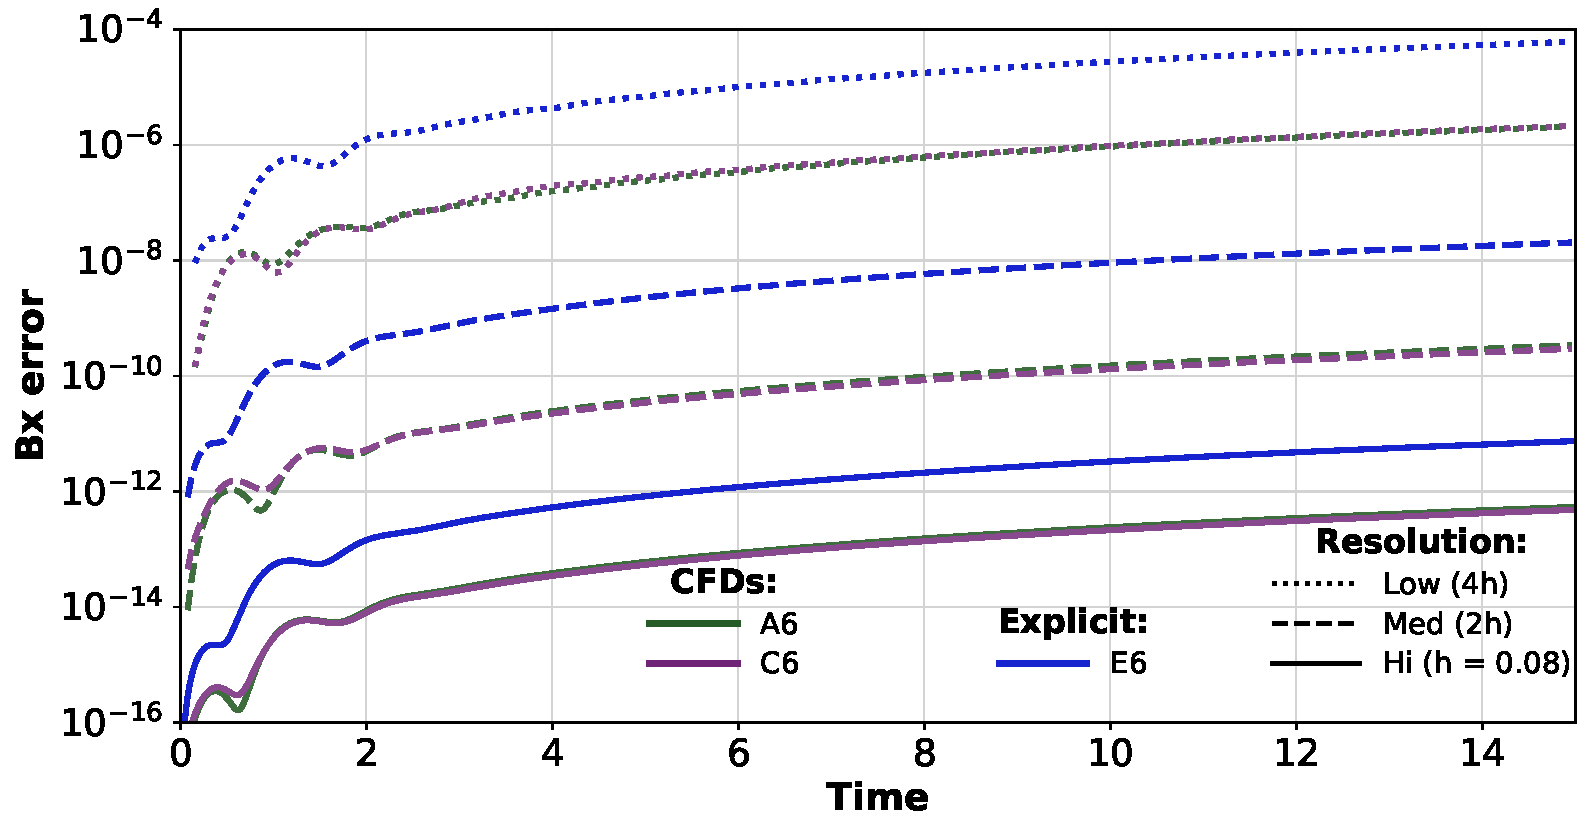
\includegraphics[width=\linewidth]{figures/6th_order_EM4_U_B0_DIFF_ALL_FAMILIES.pdf}
    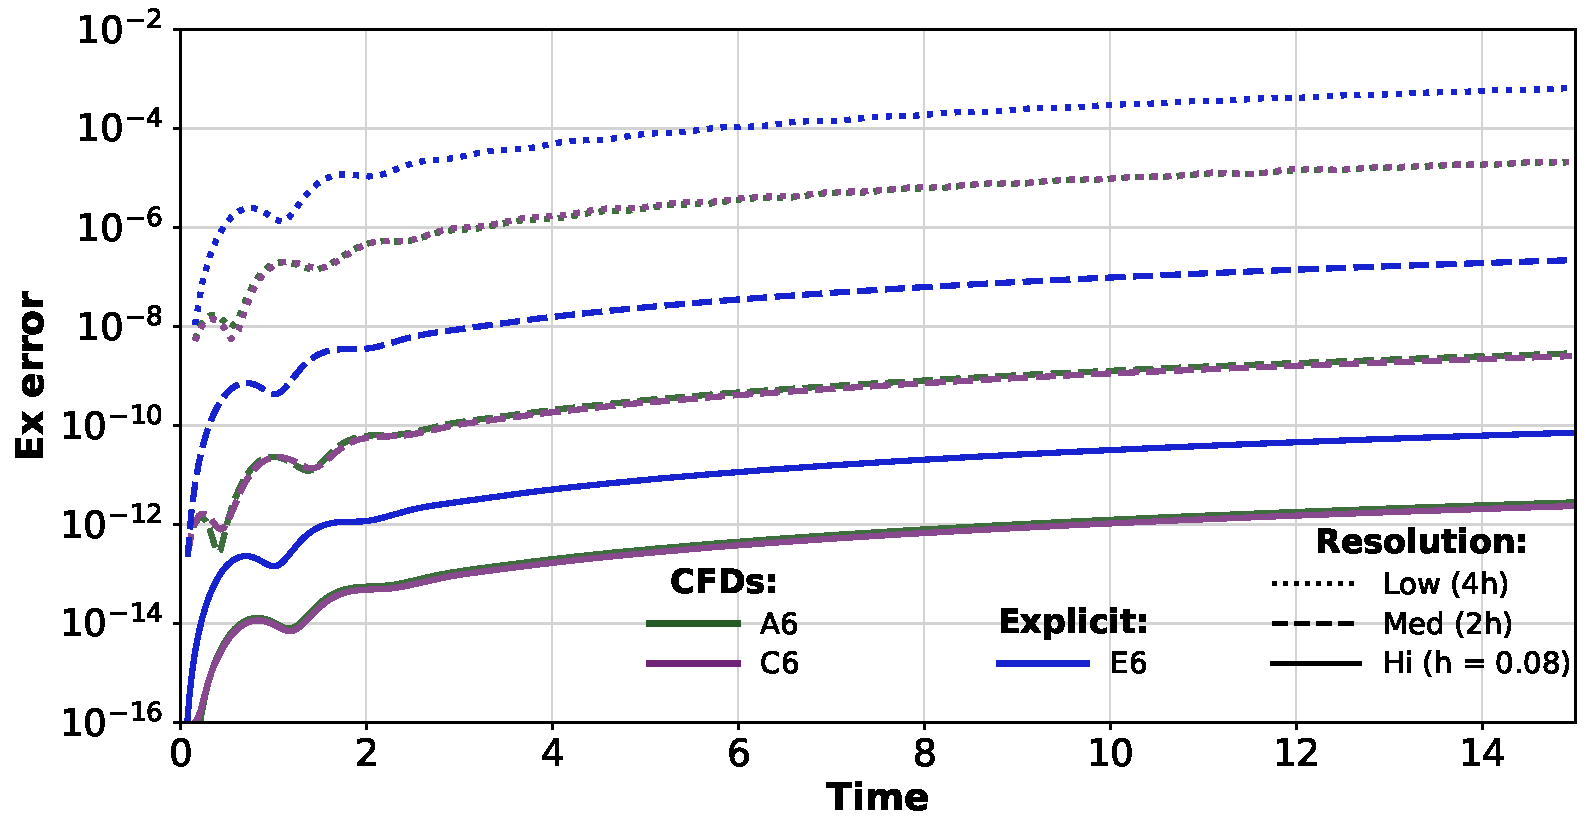
\includegraphics[width=\linewidth]{figures/6th_order_EM4_U_E0_DIFF_ALL_FAMILIES.pdf}
    %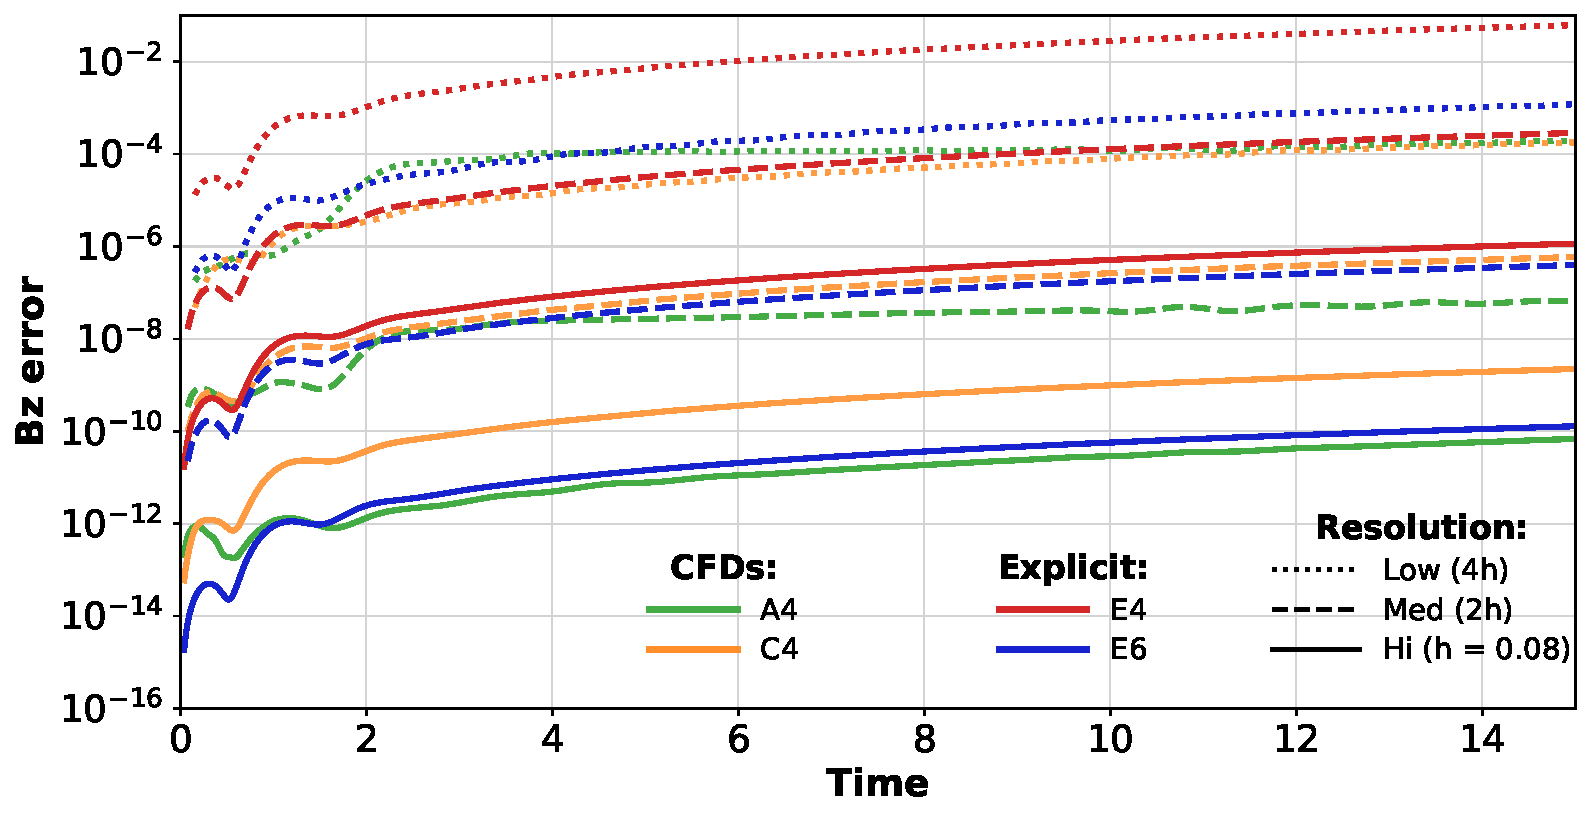
\includegraphics[width=\linewidth]{figures/U_B2_DIFF__ALL_FAMILIES.pdf}
    \vspace{-.75cm}
    \caption{
    Comparison of the errors in the magnetic and electric field components,
    $B_x$ and $E_x$, for different sixth order compact and explicit finite
    difference schemes. We plot the $L_2$ error of the numerical solution
    across the grid relative to the analytic solution. Dotted lines denote
    the low resolution runs, dashed lines denote the medium resolution runs,
    and solid lines denote the high resolution runs. The grid spacing is
    halved between each successive resolution. Although the sixth order
    compact operators do not provide a full factor of two improvement in
    resolution over their explicit counterparts of the same order, they
    still produce more than an order of magnitude improvement in accuracy.
    This behavior is observed for both the A6 and C6 families of operators
    tested here.
    }
    \label{fig:maxwell_sixth_order_error}
\end{figure}
% \begin{figure}\centering
%   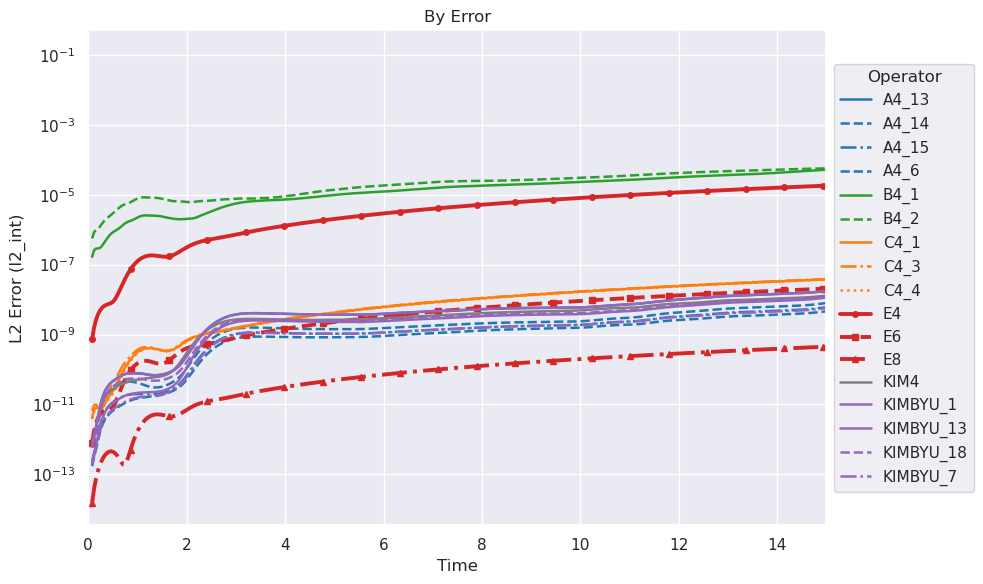
\includegraphics[width=\linewidth]{figures/U_B1_DIFF_error_plots.png}
%   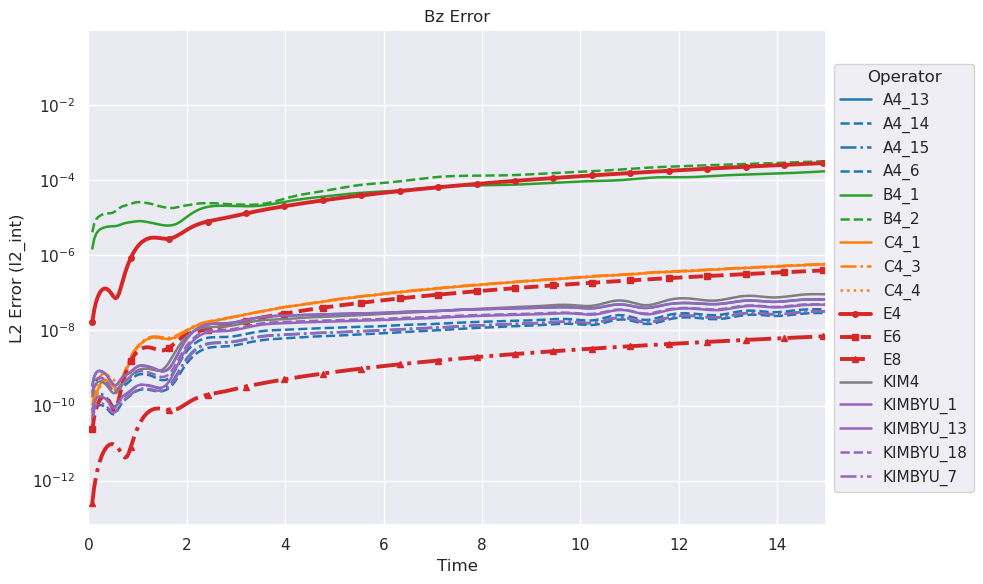
\includegraphics[width=\linewidth]{figures/U_B2_DIFF_error_plots.png}
%   \vspace{-.75cm}
%   \caption{
%     Comparison of error in the magnetic field component, $B_y$, for different CFD and explicit schemes.   component  for $q=4$. 
%     % describe sub-plots
%     We see . 
%   }
%   \label{fig:B_y_Bz_error}
% \end{figure}
% \subsection{Maxwell with second derivatives}
% \ajc{I include these here the 4th order derivatives are fine but I think that the 6th order derivatives really sell us short so I think we may be better sticking to NLSM... but they are here if we change our mind}
% \subsection{4th-order operators}
% \begin{figure}\centering
%   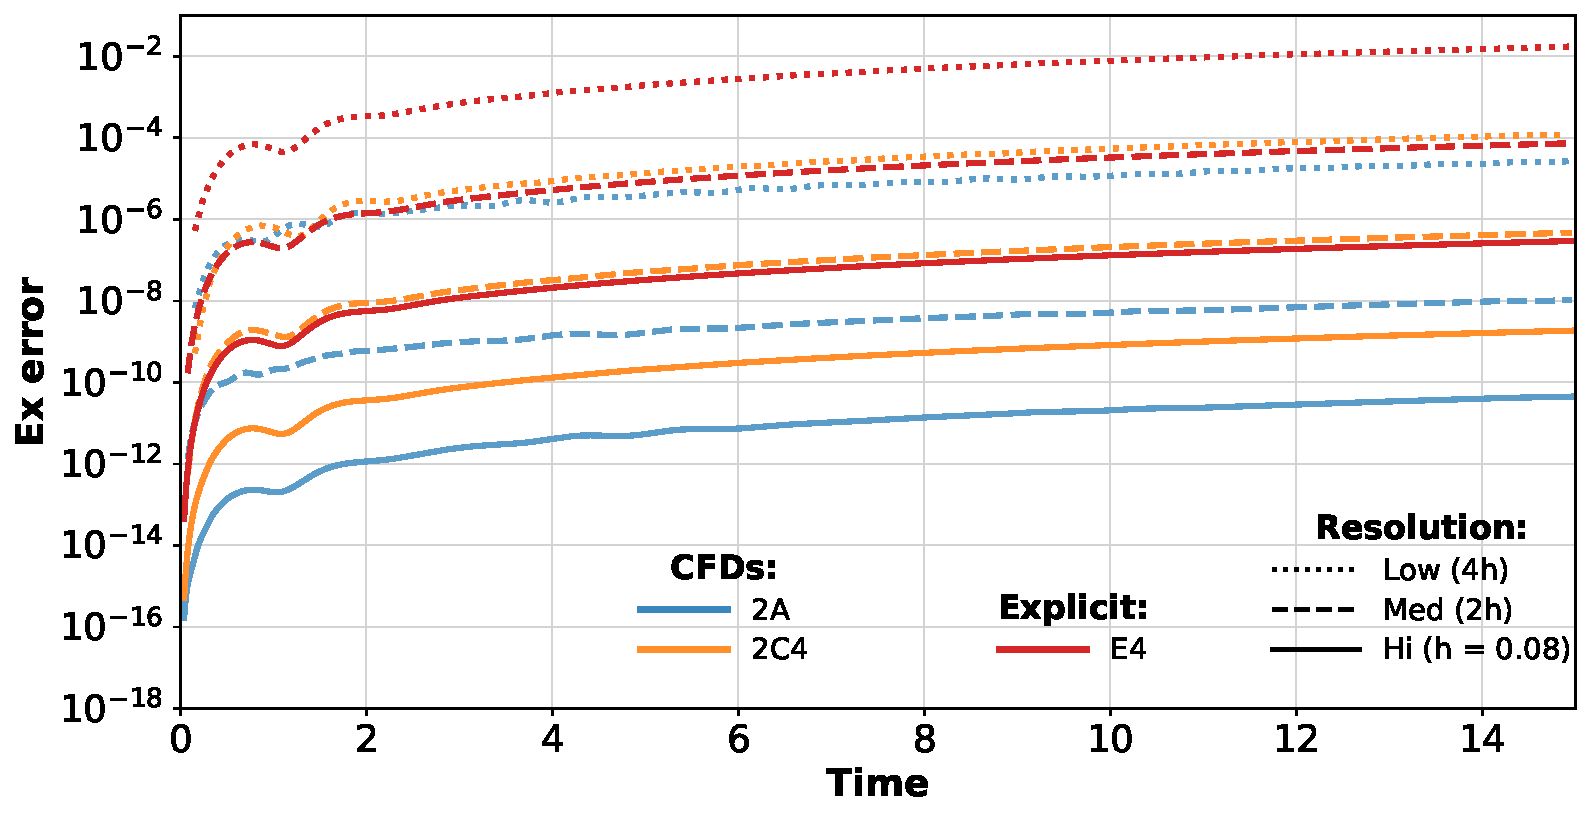
\includegraphics[width=\linewidth]{figures/4th_order_EM2_U_E0_DIFF__ALL_FAMILIES.pdf}
%   %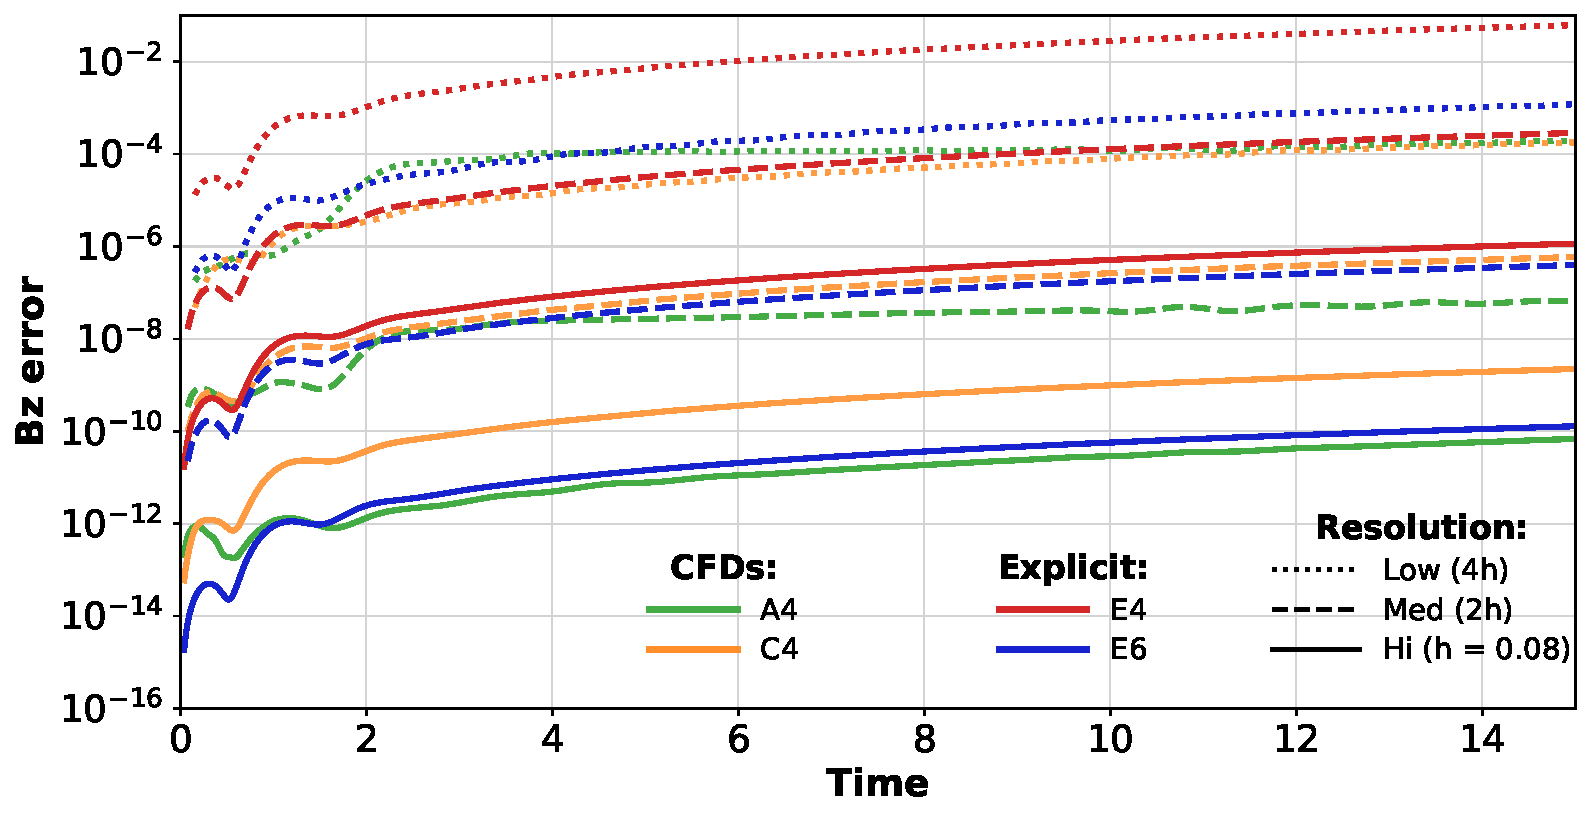
\includegraphics[width=\linewidth]{figures/U_B2_DIFF__ALL_FAMILIES.pdf}
%   \vspace{-.75cm}
%   \caption{
%    Error plot of 4th order derivatives with the second derivative formulation of Maxwell at different resolutions
% }
%   \label{fig:4th_phi_error}
% \end{figure}
% \subsection{Sixth-order operators}
% \begin{figure}\centering
%   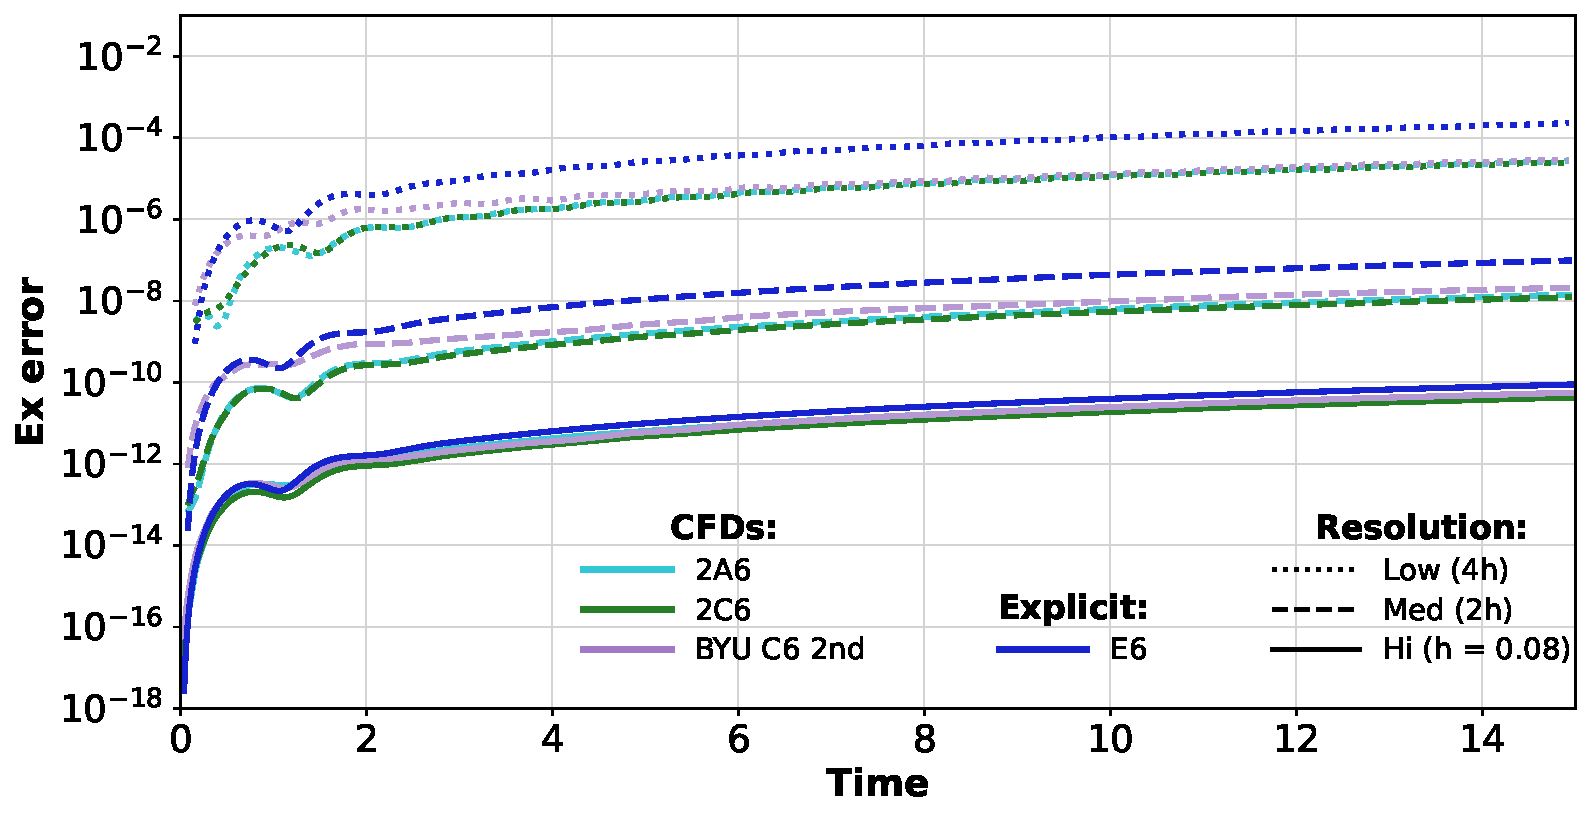
\includegraphics[width=\linewidth]{figures/6th_order_EM2_U_E0_DIFF__ALL_FAMILIES.pdf}
%   %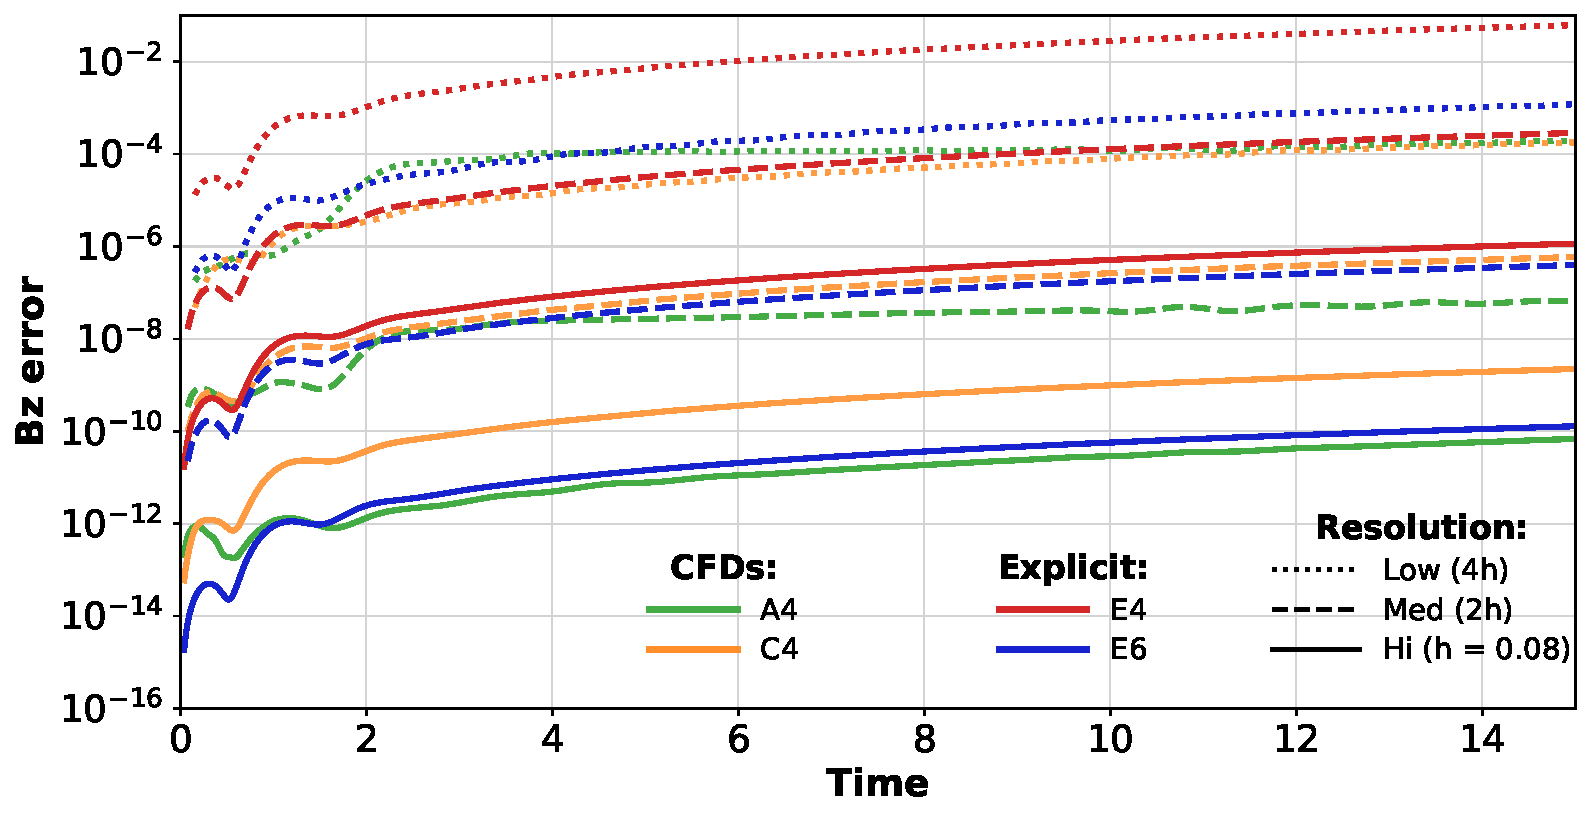
\includegraphics[width=\linewidth]{figures/U_B2_DIFF__ALL_FAMILIES.pdf}
%   \vspace{-.75cm}
%   \caption{
%  Error plot of 6th order derivatives with the second derivative formulation of Maxwell at different resolutions
% }
%   \label{fig:6th_phi_error}
% \end{figure}

\subsection{Nonlinear sigma model}

We next consider the nonlinear sigma model.  This system provides a nonlinear scalar-field test problem and is useful for studying how the different derivative operators behave in the presence of nonlinear source terms.  We evolve the scalar field $\chi$ together with its conjugate momentum $\phi$.

The evolution equations are
\begin{align}
\partial_t \phi
&= \partial_i\partial_i \chi - \frac{\sin(2\chi)}{r^2},
\\
\partial_t \chi
&= \phi .
\end{align}
Here $\partial_i\partial_i$ denotes the flat-space Laplacian.  The term $\sin(2\chi)/r^2$ provides a useful test of the stability and accuracy of the numerical method in nonlinear systems.
In this case we don't have an analytic solution but we do a few convergence tests shown in figure blah. This gives us the change to confirm that our operators work even in a nonlinear system and converge at the expected order.  We use initial data given as follows:
 The scalar field is initialized as
\begin{equation}
\chi(x,y,z)
=
A
\exp\left[
-\frac{(\tilde r-R)^2}{\delta^2}
\right],
\end{equation}
where
\begin{equation}
\tilde r
=
\sqrt{
\epsilon_x(x-x_c)^2
+
\epsilon_y(y-y_c)^2
+
\epsilon_z(z-z_c)^2
}.
\end{equation}
The conjugate momentum is initially set to
\begin{equation}
\phi(x,y,z)=0.
\end{equation}

For the simulations considered here, we choose
\begin{equation}
A=1,\qquad
\delta=3,\qquad
x_c=y_c=z_c=0,
\end{equation}
together with
\begin{equation}
\epsilon_x=\epsilon_y=\epsilon_z=1,
\qquad
R=0.
\end{equation}
Thus, the initial scalar profile is a spherically symmetric Gaussian centered
at the origin. The wave speeds in all three spatial directions are set to
unity.
%\ajc{I have added in convergence plots, I will probably update these but the story shouldn't change too much}

\paragraph{Fourth Order Operators}

\begin{figure}[t]
    \centering
    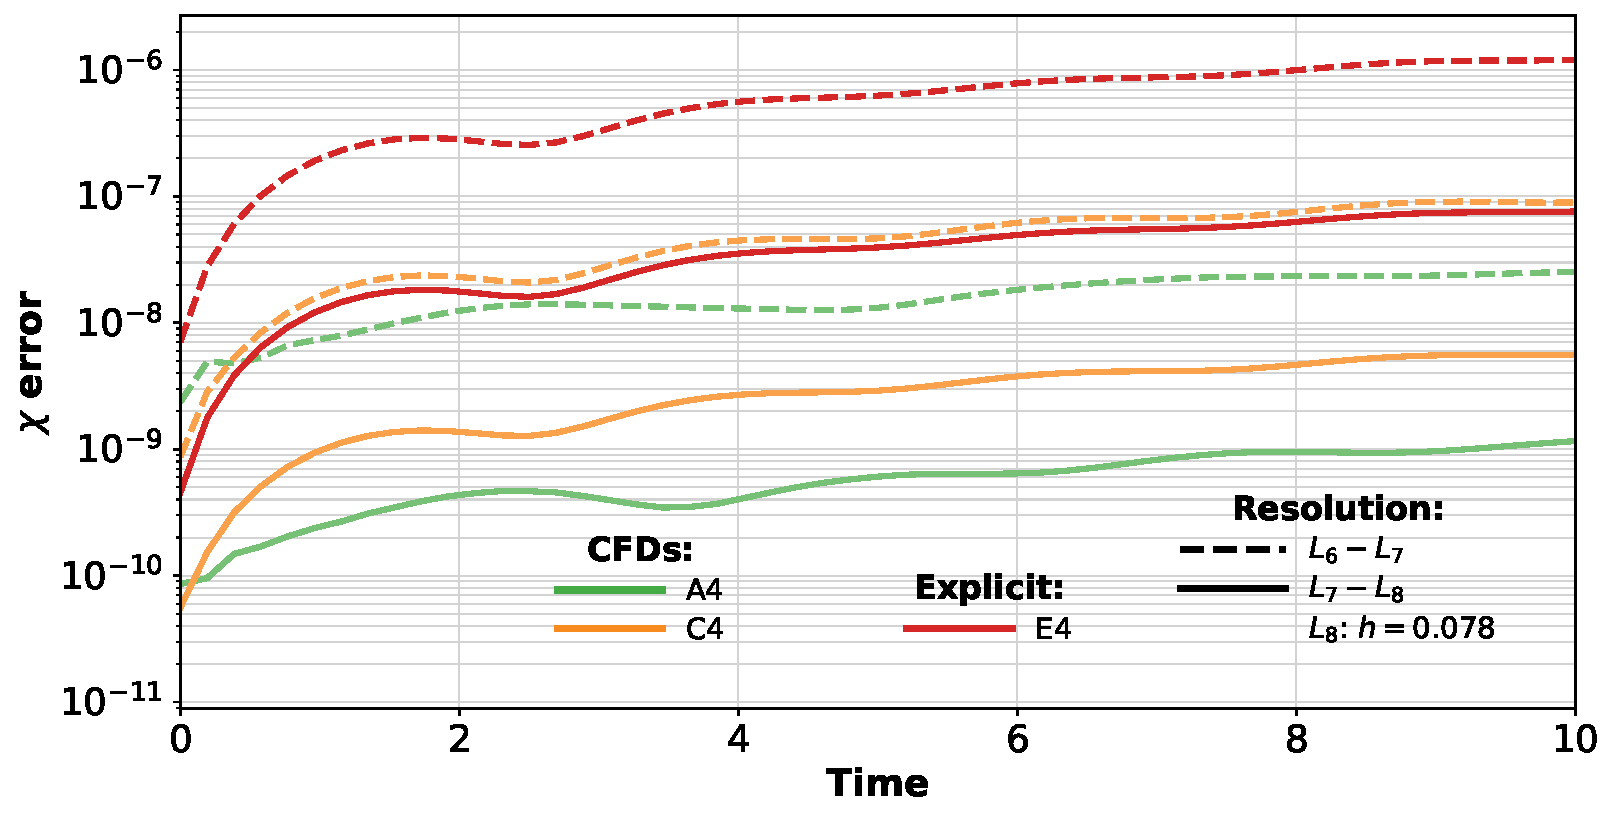
\includegraphics[width=\linewidth]{figures/4th_order_U_CHI_ALL_FAMILIES.pdf}
    %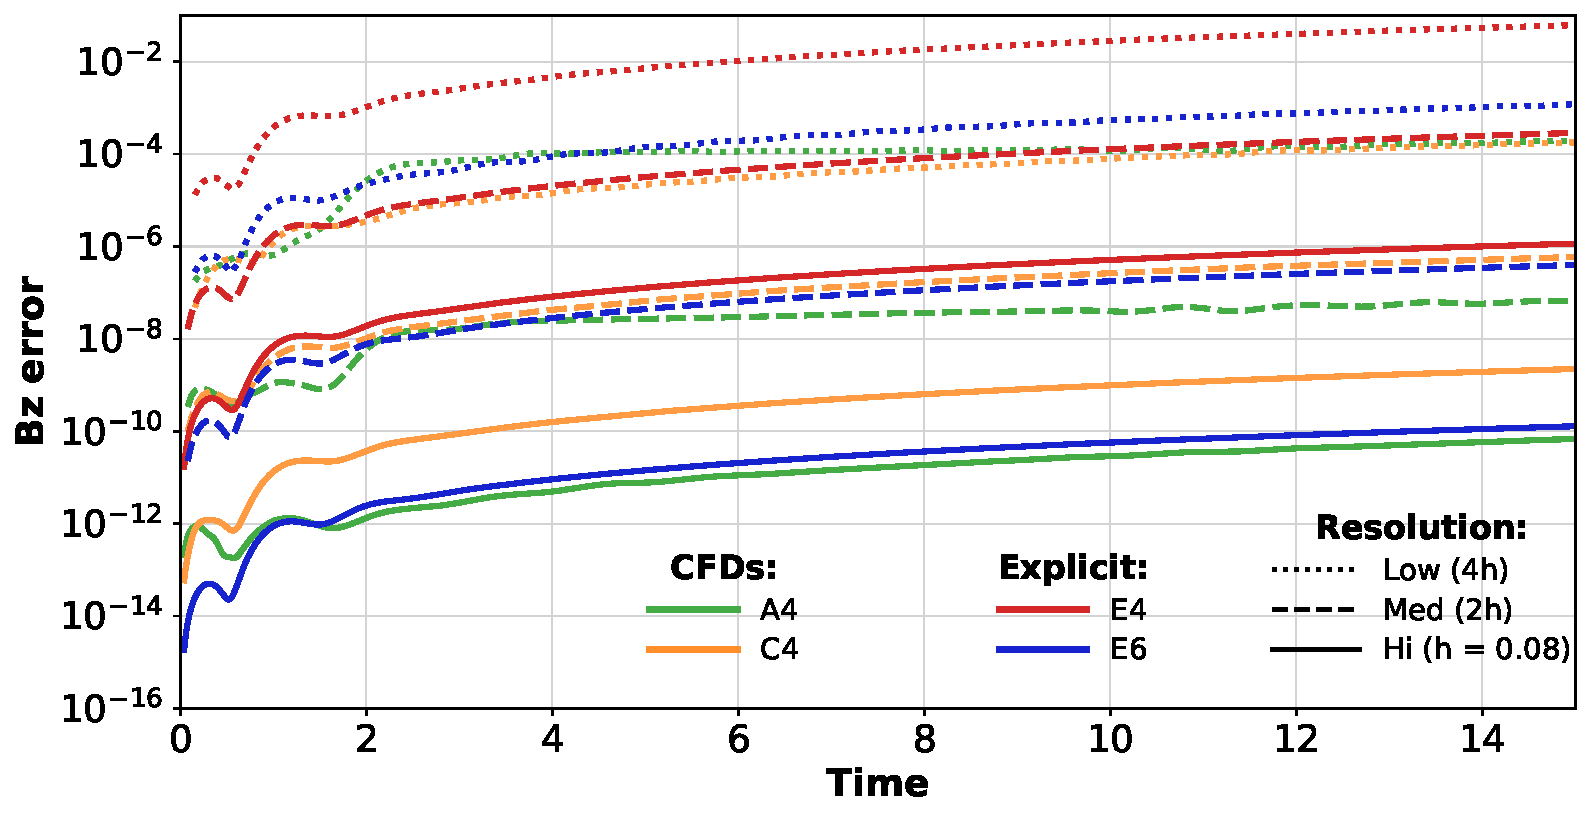
\includegraphics[width=\linewidth]{figures/U_B2_DIFF__ALL_FAMILIES.pdf}
    \vspace{-.75cm}
    \caption{
    Convergence of the nonlinear sigma model field $\phi$ for the fourth
    order compact and explicit finite difference schemes. The plotted
    quantity is the difference between successive resolutions. Dotted lines
    denote the low and medium resolution comparison, dashed lines denote the
    medium and high resolution comparison, and solid lines denote the highest
    resolution run. The grid spacing is halved between each successive
    resolution. The compact operators remain stable in the nonlinear system. Notice that again in this nonlinear system the 4th order A4 and C4 operators perform the same as the Explicit 4th order at half od the resolution. 
    }
    \label{fig:nlsm_fourth_order_error}
\end{figure}

\paragraph{Sixth Order Operators}

\begin{figure}[t]
    \centering
    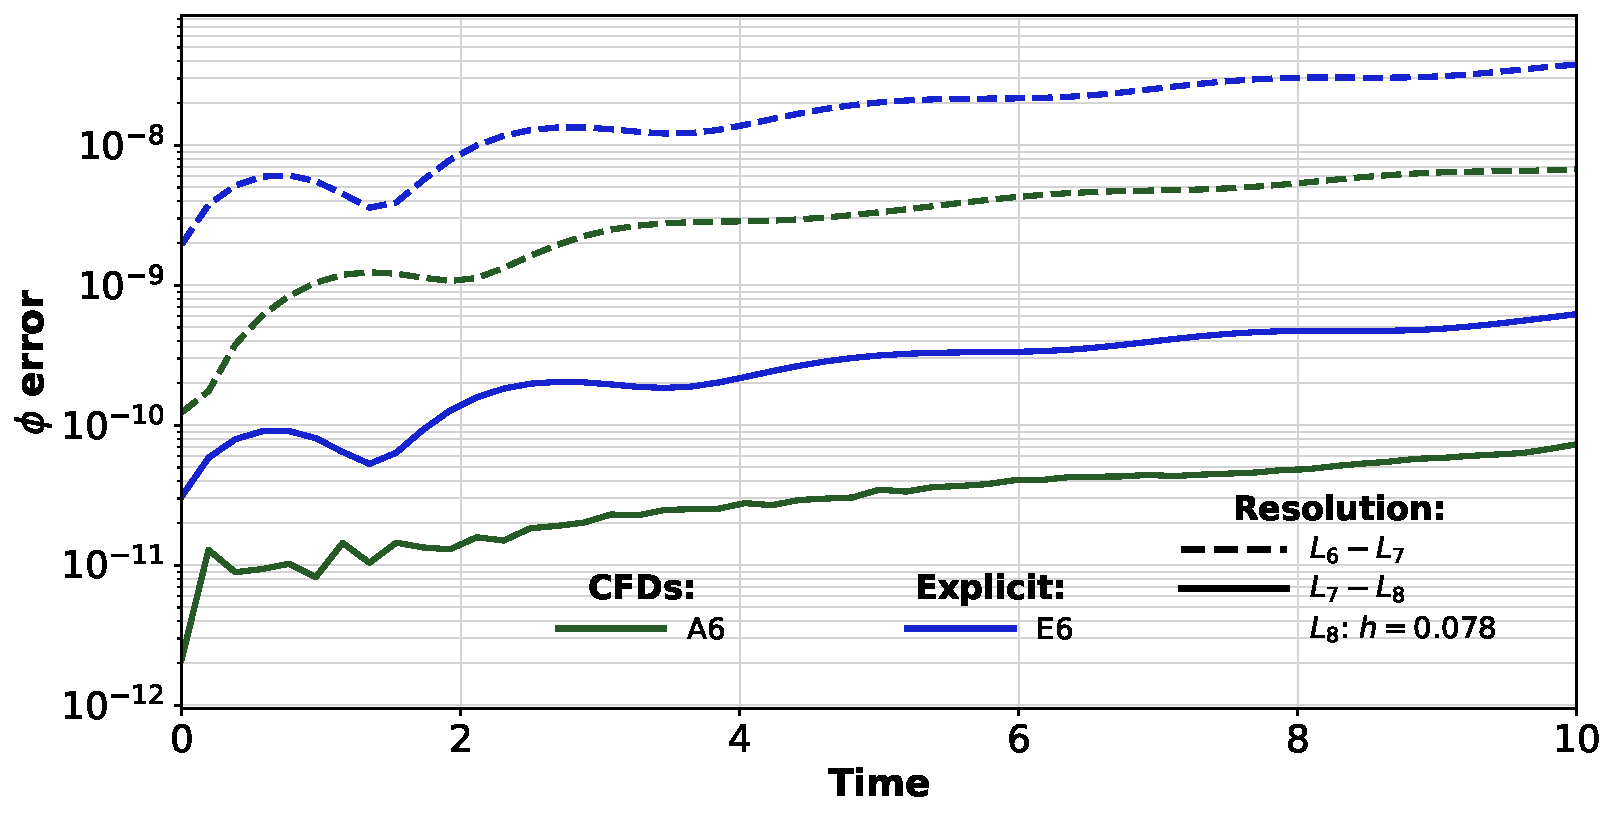
\includegraphics[width=\linewidth]{figures/6th_order_U_PHI_ALL_FAMILIES.pdf}
    %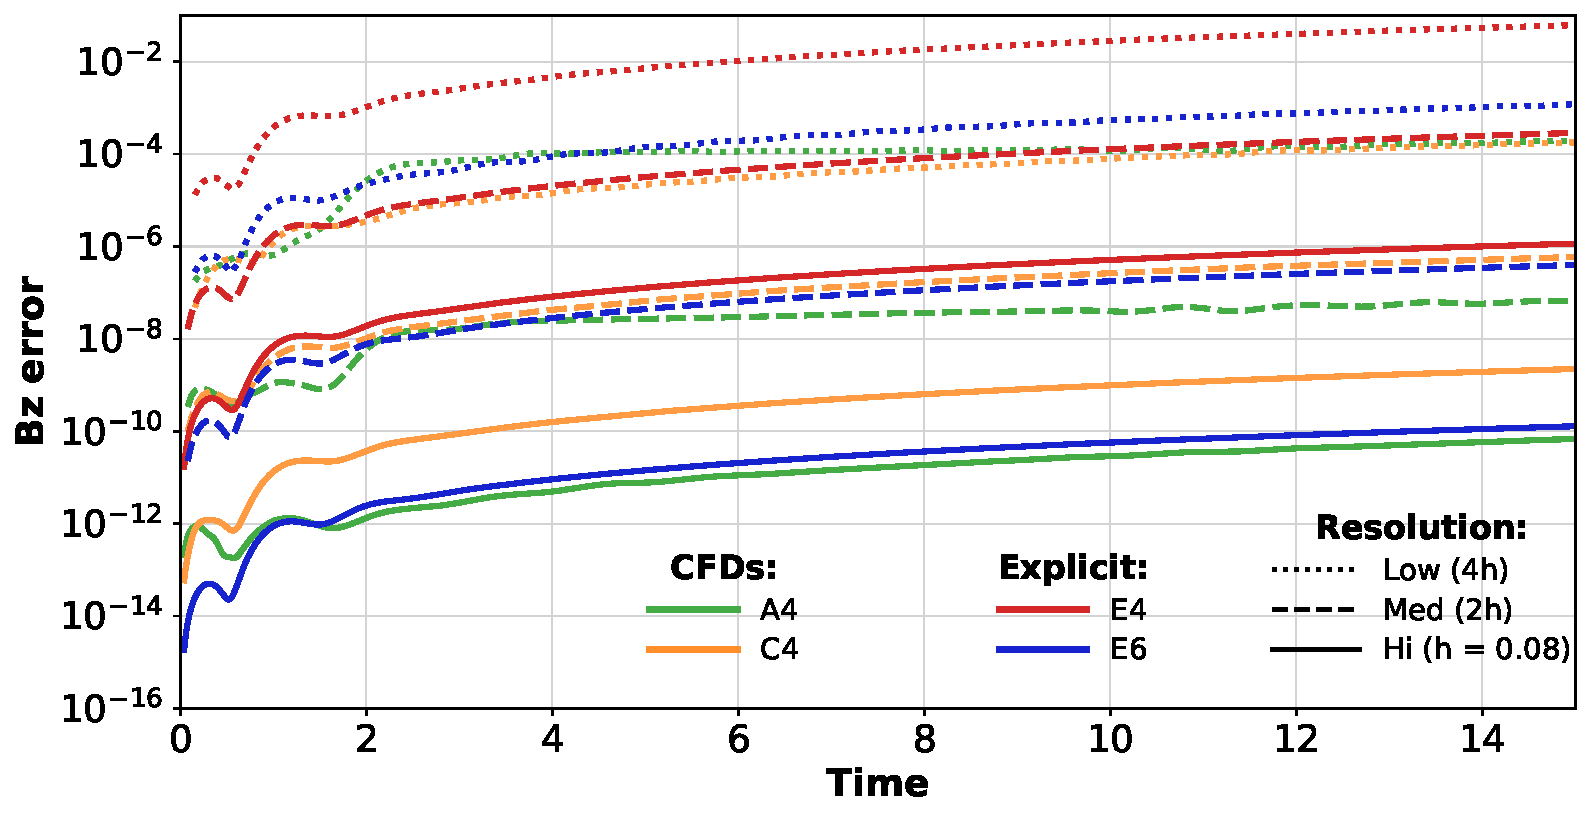
\includegraphics[width=\linewidth]{figures/U_B2_DIFF__ALL_FAMILIES.pdf}
    \vspace{-.75cm}
    \caption{
    Convergence of the nonlinear sigma model field $\phi$ for the sixth
    order compact and explicit finite difference schemes. The plotted
    quantity is the difference between successive resolutions. Dotted lines
    denote the low and medium resolution comparison, dashed lines denote the
    medium and high resolution comparison, and solid lines denote the highest
    resolution run. The grid spacing is halved between each successive
    resolution. We do not seem to get the full order of resolution improvement that we got with the 4th order operators but we do seem to get close to an order of magnitude improvement..
    }
    \label{fig:nlsm_sixth_order_error}
\end{figure}
\subsection{Gravitational Waves}

We also test the derivative operators by evolving Teukolsky-wave initial data with the full BSSN equations.  The BSSN formulation is described in detail elsewhere, for example in Ref.~\cite{Baumgarte2010}.  These data describe a linearized gravitational-wave perturbation of the metric and provide a useful test problem for wave propagation in a numerical relativity setting.

For the results shown here, we perform direct convergence tests rather than
comparing against an analytic solution. The computational domain extends over
$x,y,z\in[-40,40]$, and the initial perturbation is centered at radius
$r_0=20.0$. We use outgoing, even-parity Teukolsky-wave initial data in the
quadrupolar mode $(\ell,m)=(2,0)$ with amplitude $\mathcal{A}=10^{-2}$. The
radial profile is a compactly supported $C^k$ polynomial with $k=6$ and
half-width $w=2.0$. A representative visualization of the resulting evolution
is shown in Fig.~\ref{fig:bssn_gt00_panel}.

\begin{figure}[t]
    \centering
    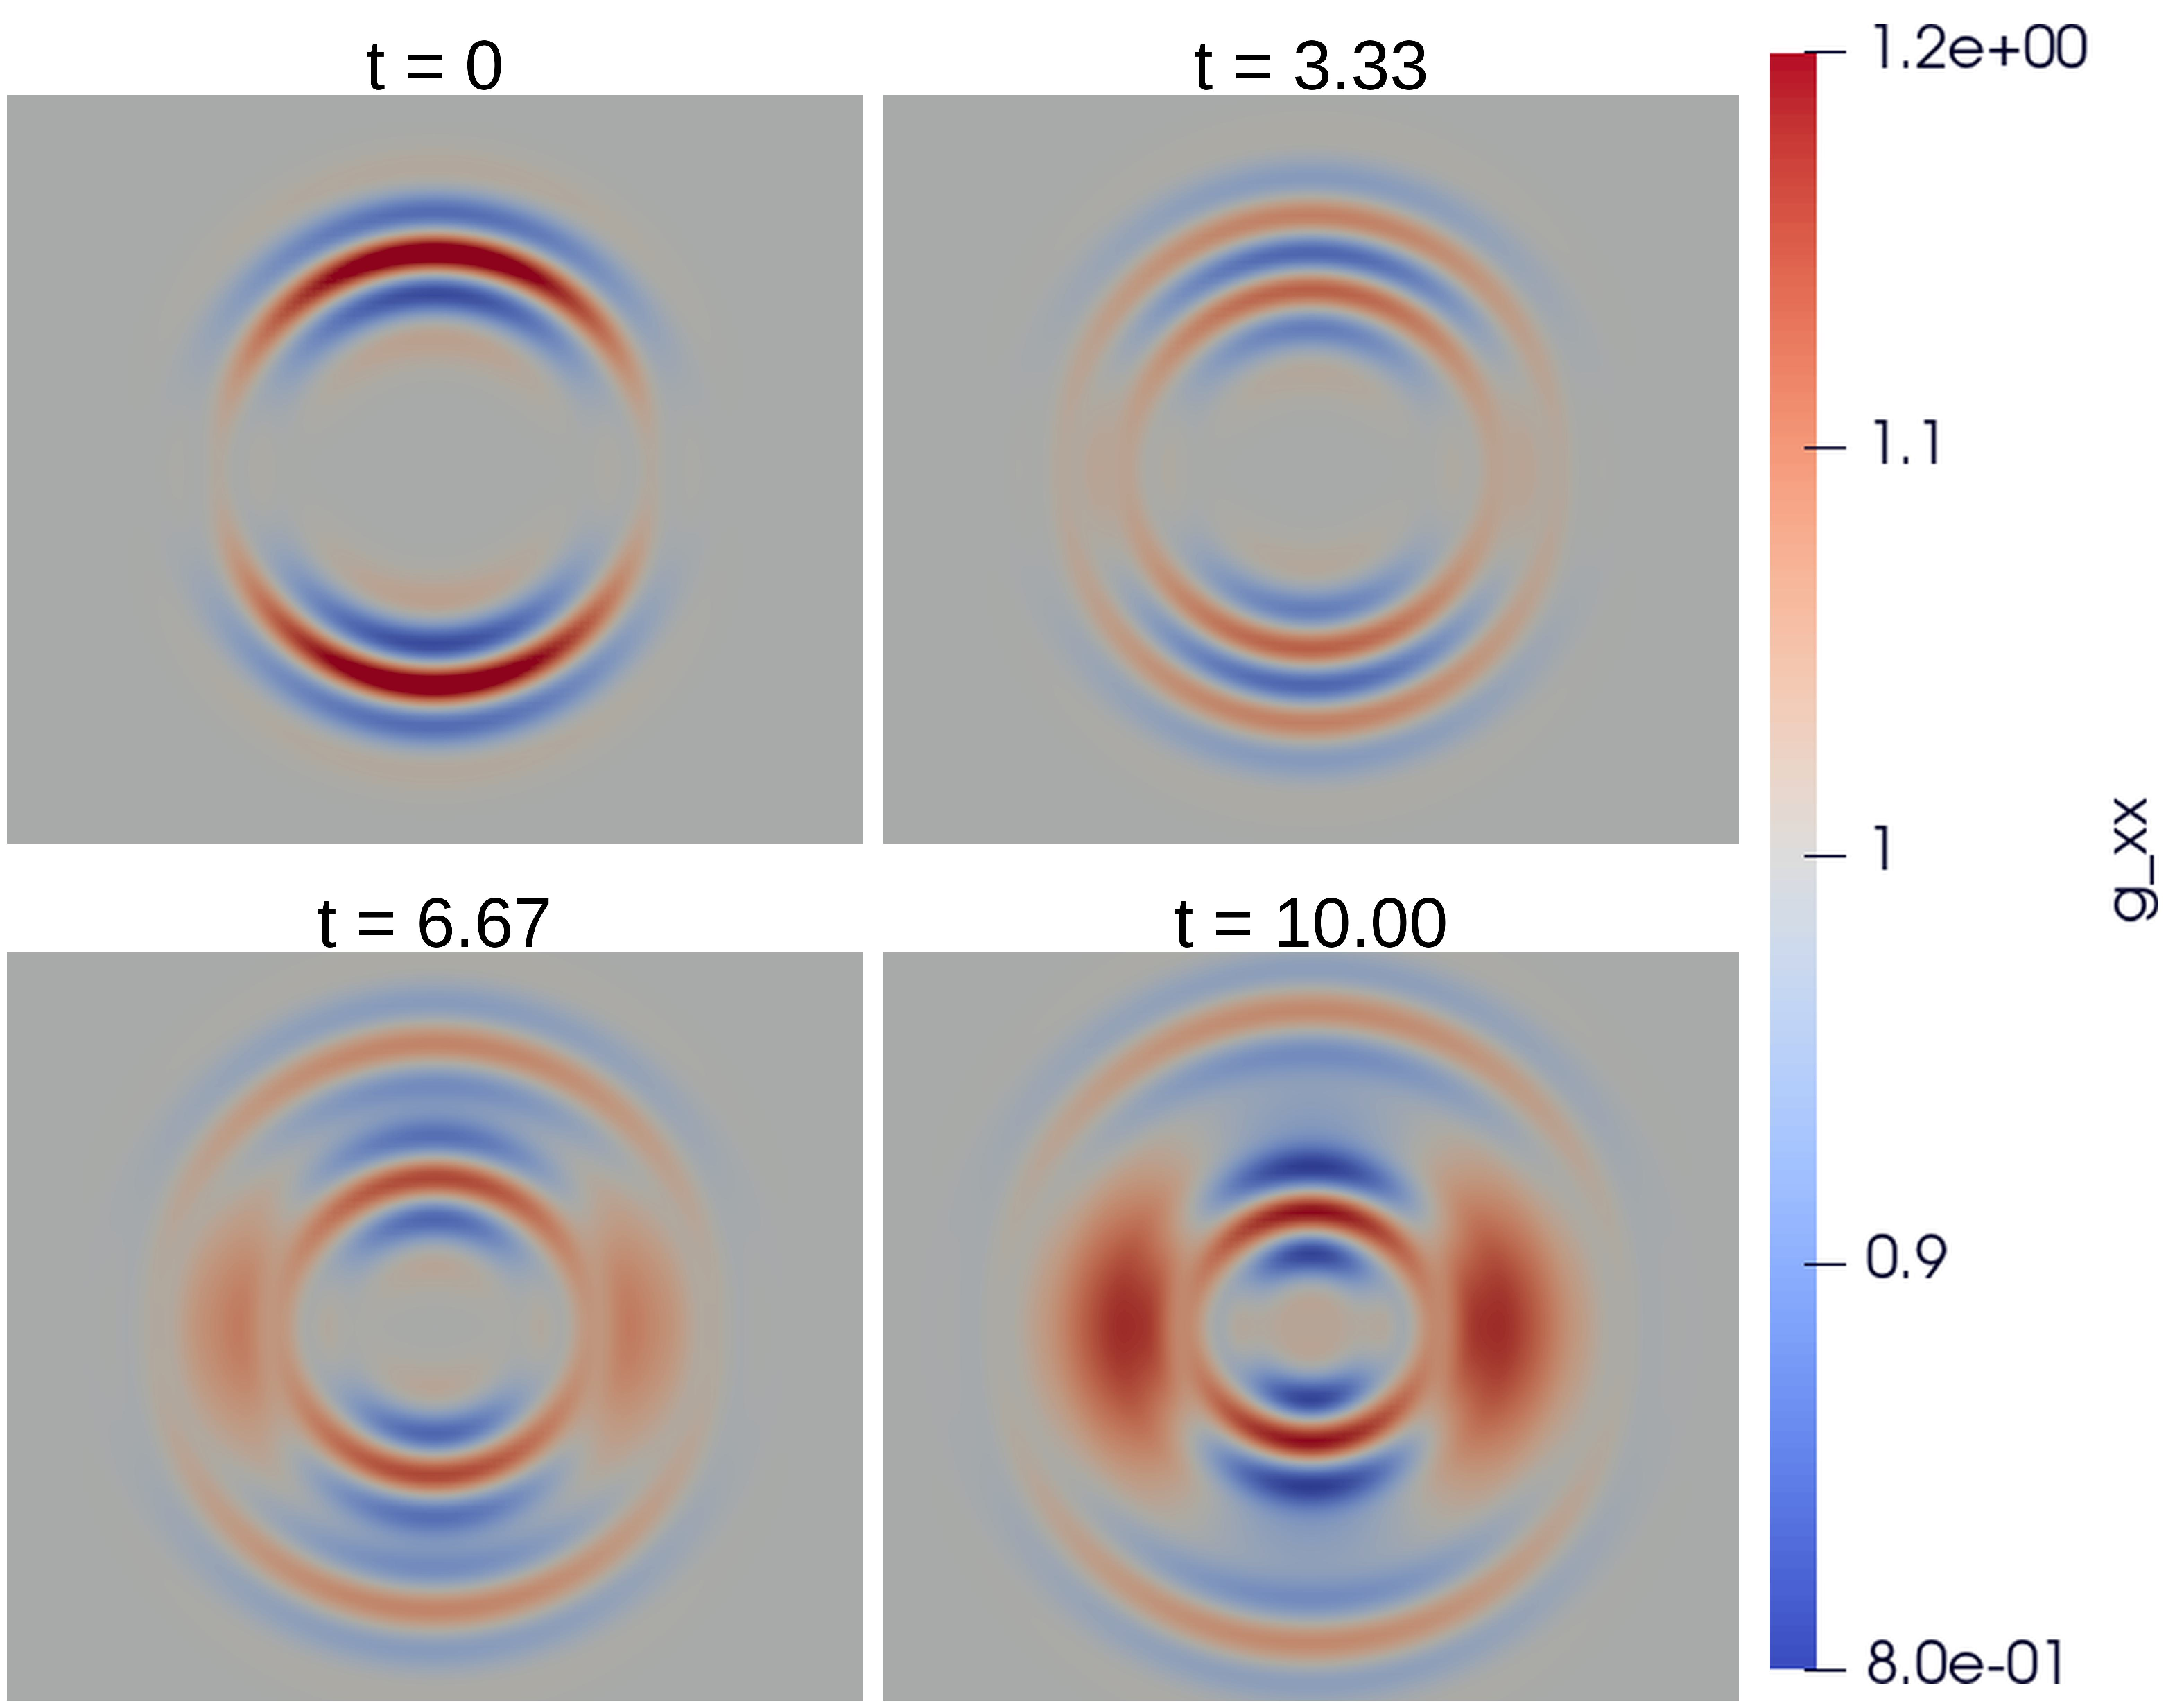
\includegraphics[width=\columnwidth]{figures/GT00_panel.pdf}
    \caption{
    Evolution of the metric component $g_{xx}$ for the Teukolsky-wave test problem.
    The panels show snapshots at $t=0$, $t=3.33$, $t=6.67$, and $t=10.00$.
    The shared color scale on the right applies to all four panels.
    }
    \label{fig:bssn_gt00_panel}
\end{figure}

\paragraph{Fourth Order Operators}

\begin{figure}[t]
    \centering
    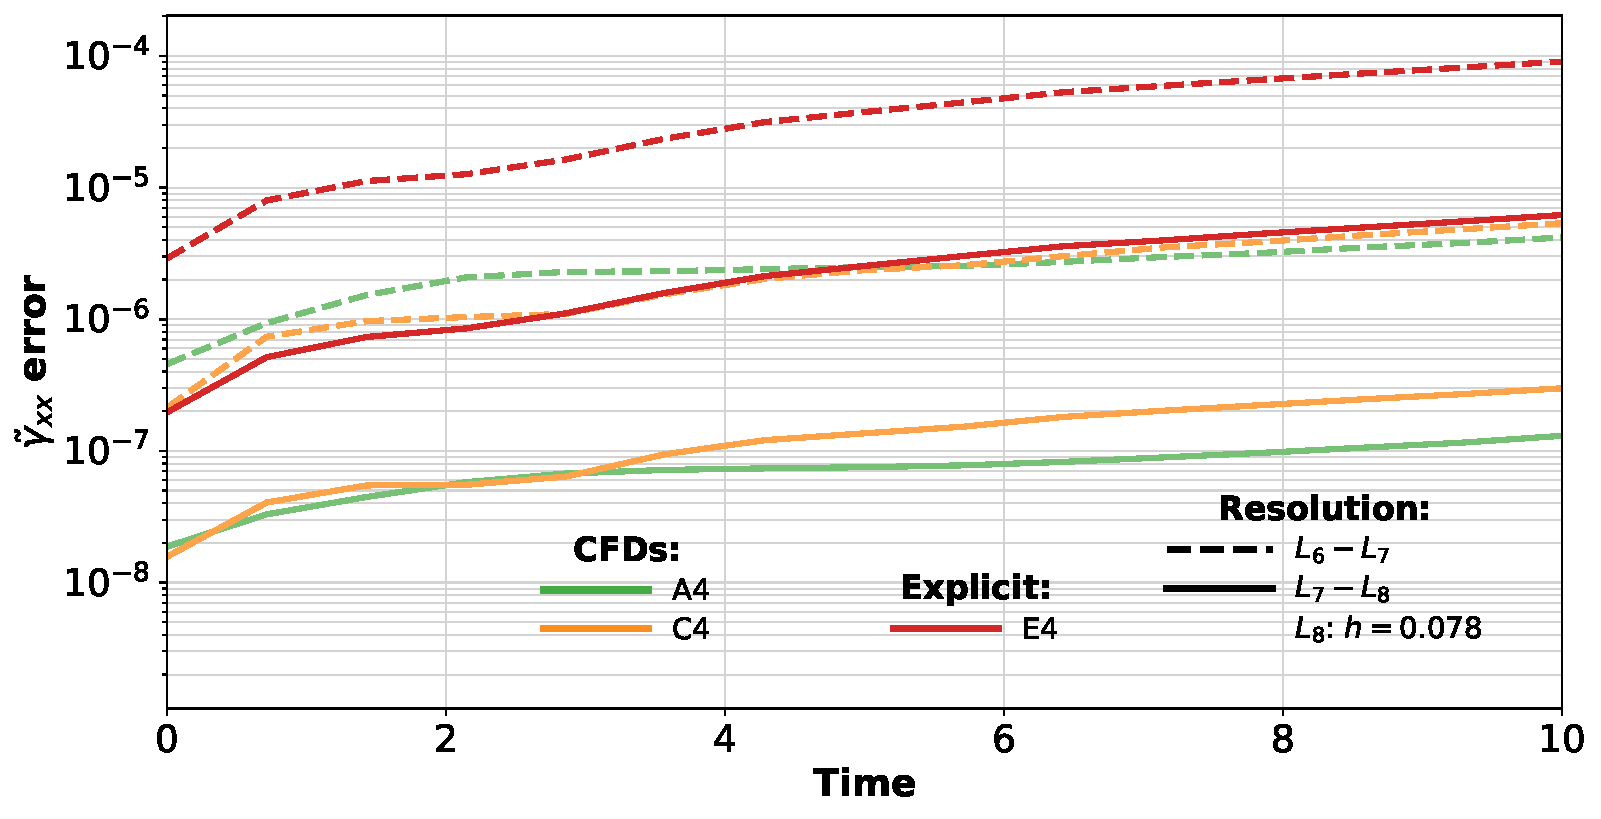
\includegraphics[width=\linewidth]{figures/4th_order_U_SYMGT0_ALL_FAMILIES.pdf}
    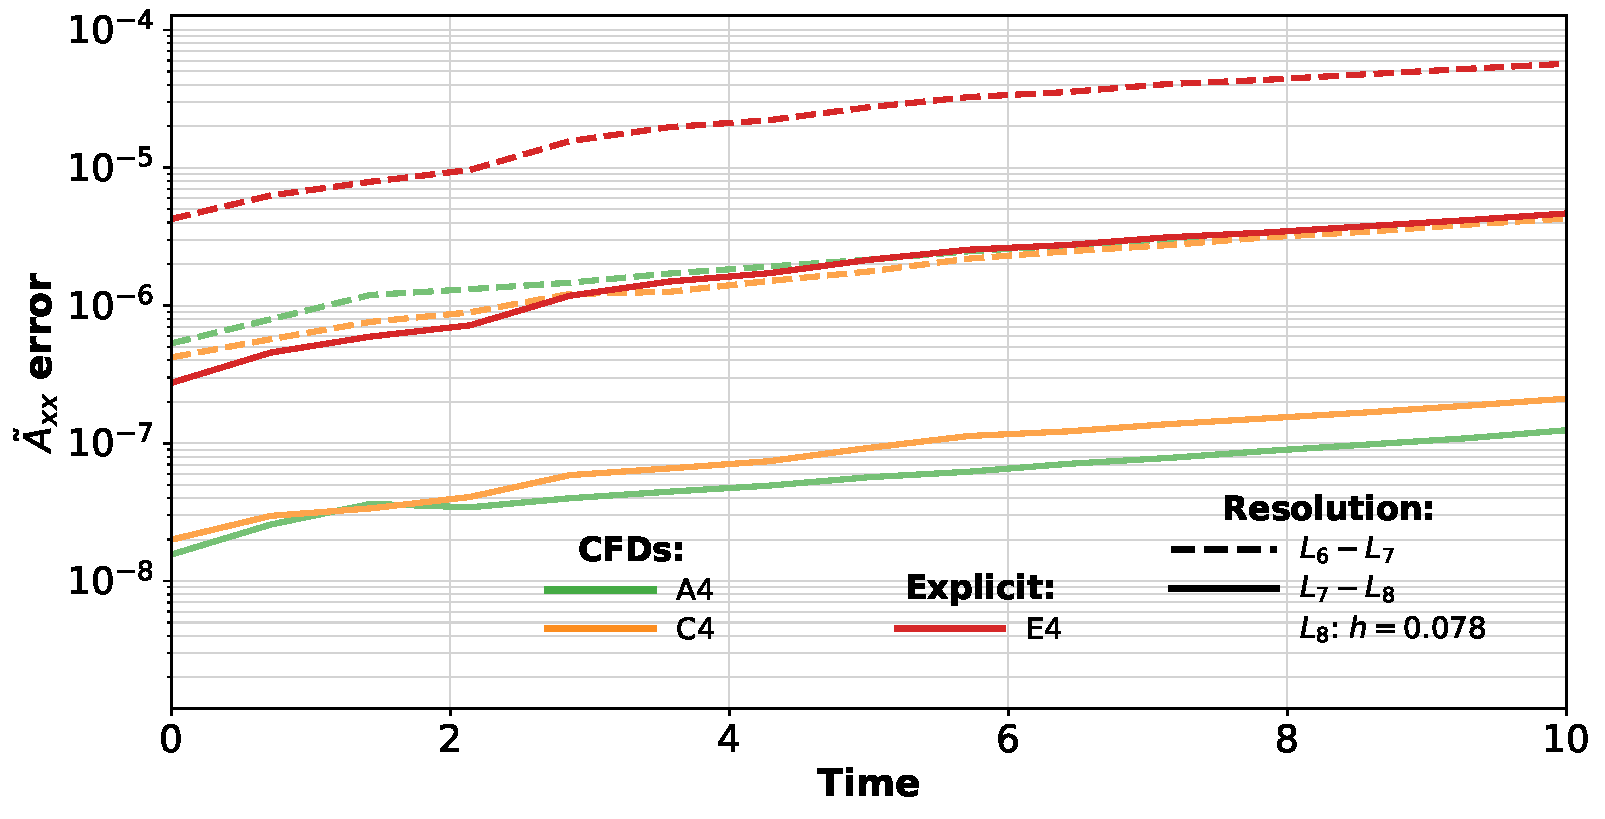
\includegraphics[width=\linewidth]{figures/4th_order_U_SYMAT0_ALL_FAMILIES.pdf}
    \vspace{-.75cm}
    \caption{
    Convergence of the metric component $g_{xx}$ and the conformal extrinsic
    curvature component $\tilde{A}_{xx}$ for the fourth order compact and
    explicit finite difference schemes. The plotted quantities are the
    differences between successive resolutions. Dotted lines denote the low
    and medium resolution comparison, dashed lines denote the medium and high
    resolution comparison, and solid lines denote the highest resolution run.
    The grid spacing is halved between each successive resolution. The compact
    operators remain stable during the Teukolsky wave evolution. Notice that,
    as in the nonlinear sigma model, the fourth order A4 and C4 operators
    perform comparably to the explicit fourth order operator at half the
    resolution.
    }
    \label{fig:teukolsky_fourth_order_error}
\end{figure}

\paragraph{Sixth Order Operators}

\begin{figure}[t]
    \centering
    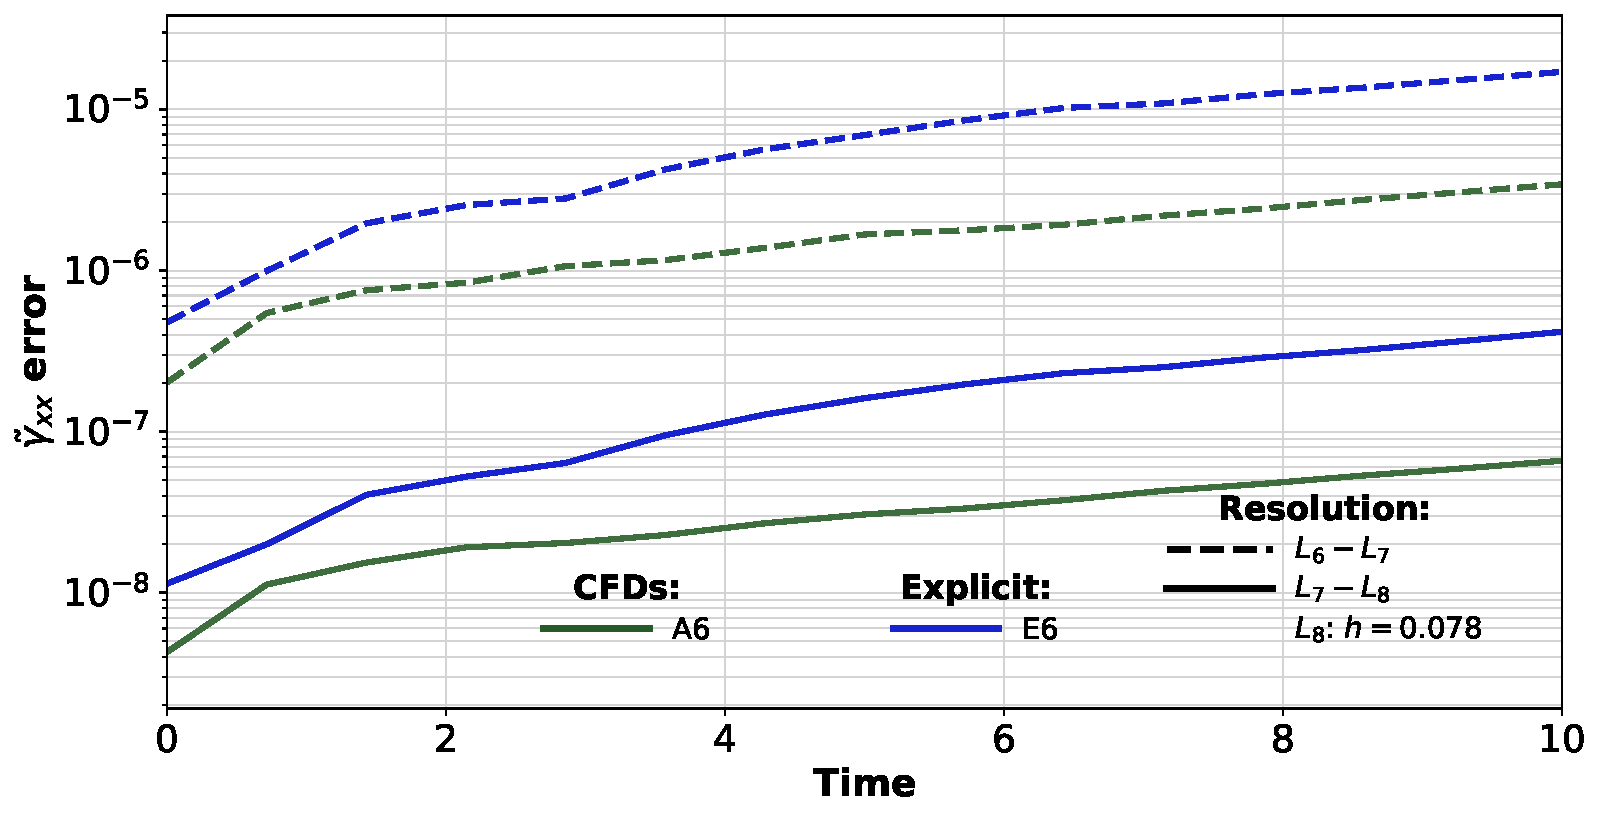
\includegraphics[width=\linewidth]{figures/6th_order_U_SYMGT0_ALL_FAMILIES.pdf}
    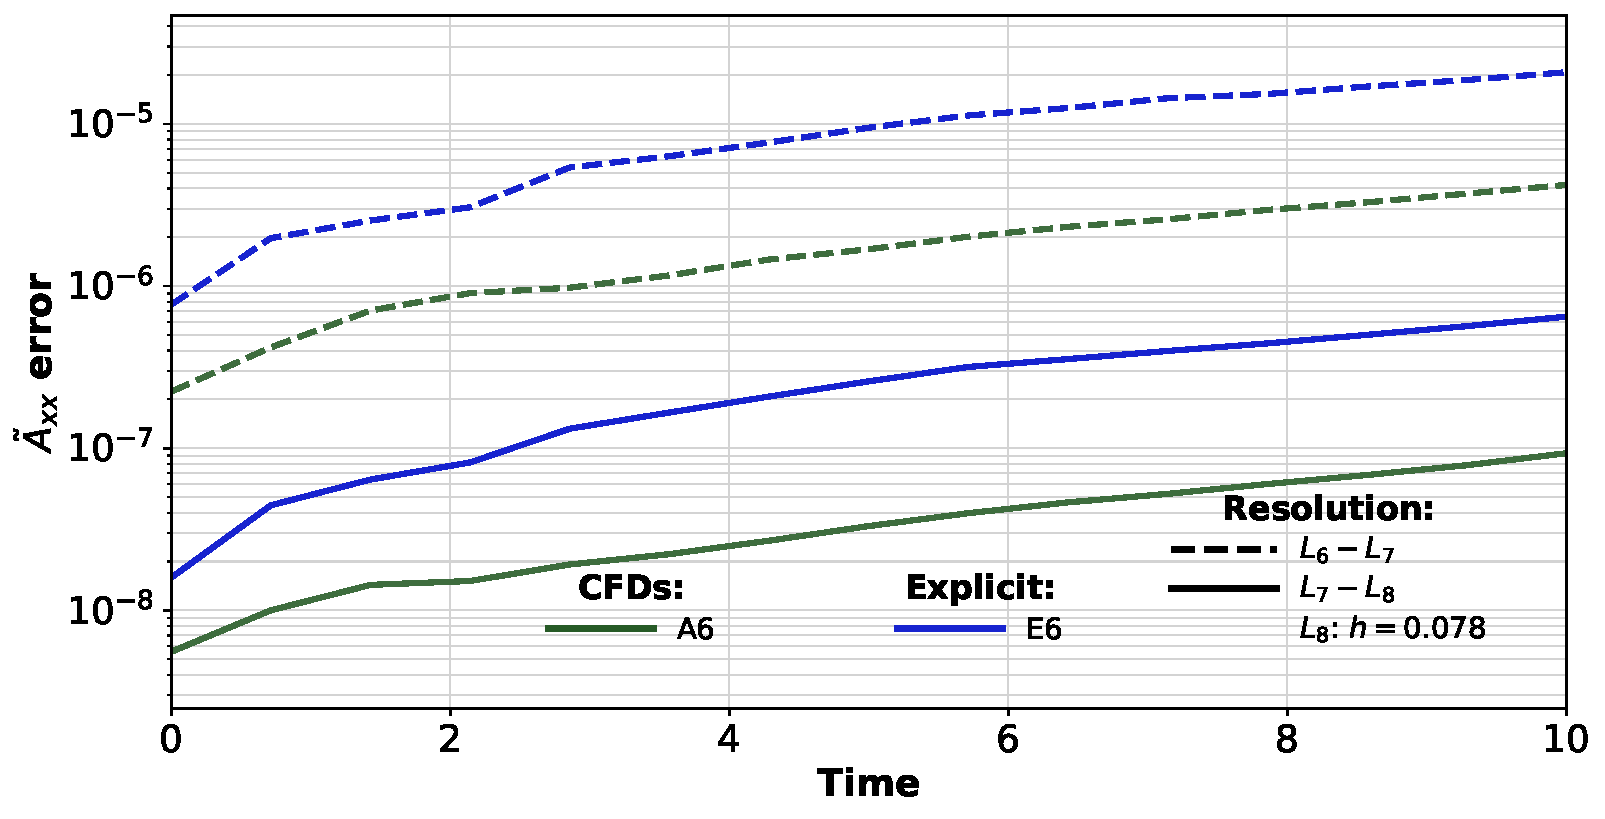
\includegraphics[width=\linewidth]{figures/6th_order_U_SYMAT0_ALL_FAMILIES.pdf}
    \vspace{-.75cm}
    \caption{
    Convergence of the metric component $g_{xx}$ and the conformal extrinsic
    curvature component $\tilde{A}_{xx}$ for the sixth order compact and
    explicit finite difference schemes. The plotted quantities are the
    differences between successive resolutions. Dotted lines denote the low
    and medium resolution comparison, dashed lines denote the medium and high
    resolution comparison, and solid lines denote the highest resolution run.
    The grid spacing is halved between each successive resolution. As in the
    nonlinear sigma model, the sixth order compact operators do not achieve
    the full resolution improvement seen for the fourth order operators, but
    they still provide close to an order of magnitude improvement in accuracy.
    }
    \label{fig:teukolsky_sixth_order_error}
\end{figure}
\section{Conclusion}
\label{sec:conclusion}

The compact operators consistently produced smaller errors than explicit
finite difference operators of the same nominal order. In the fourth order
tests, the compact operators frequently achieved errors comparable to those
of the explicit operators evaluated at twice the resolution. They also
produced error levels comparable to sixth order explicit operators in several
of the Maxwell tests. The sixth order compact operators did not always provide
a full factor of two improvement in effective resolution, but they commonly
reduced the error by approximately an order of magnitude relative to their
explicit counterparts.

These improvements were observed in the Maxwell system, the nonlinear sigma
model, and evolutions of Teukolsky gravitational wave initial data using the
BSSN equations. The results therefore indicate that the benefits of the
compact operators are not limited to simple linear systems. In particular,
the operators remained stable and retained their accuracy improvements in
nonlinear and numerical relativity test problems.

Compact finite differences require the solution of an implicit matrix system,
but the fixed size leaf nodes used by \dendrogr\ allow these systems to be
solved efficiently using vectorized linear algebra routines. The additional
cost of the compact derivative calculation may therefore be offset by the
ability to obtain a given error at a lower grid resolution. For
three dimensional time dependent simulations, even a modest reduction in the
required resolution could lead to substantial savings in computational cost.

The next step is to apply these operators to fully nonlinear binary black hole
simulations on adaptive meshes. These tests will determine how the operators
behave near punctures, across refinement boundaries, and during long
inspiral evolutions. They will also allow direct comparisons of waveform
accuracy and computational cost between compact and explicit finite
difference methods. The results presented here suggest that compact finite
differences provide a promising route toward more accurate gravitational
waveforms without requiring a corresponding increase in computational
expense. We already have some tentative results showing that CFDs perform well
in full binary black hole systems, which we present in
Appendix~\ref{sec:black_hole_merger_tests}. In those cases, we show that the
fourth order compact operators perform better than their explicit counterparts.

\chapter{Conclusion}
\section{Conclusion}

Throughout this dissertation, we have pursued two complementary themes in numerical relativity. The first is the numerical modeling of black-hole spacetimes in Einstein--Maxwell--dilaton--axion theory, an extension of general relativity that includes electromagnetic, dilaton, and axion fields. Within this setting, we studied the nonlinear stability of charged black holes and investigated how these additional fields can affect gravitational waveforms from binary black-hole mergers. This work provides an example of how numerical relativity can be used to explore strong-field dynamics in theories beyond general relativity.

The second theme is the improvement of numerical relativity methods through the use of compact finite-difference operators. These methods are designed to improve the accuracy and efficiency of simulations of strong-field gravitational systems. In this final chapter, we summarize the main conclusions from each part of the dissertation and discuss directions for future work.

In the first EMDA portion of this dissertation, we developed a method for constructing approximate binary black-hole initial data in Einstein--Maxwell--dilaton--axion theory. This allowed us to evolve head-on collisions of charged black holes across a range of initial spins, charges, and field configurations. These simulations were used to study whether the additional fields present in EMDA theory remain associated with black holes in the fully nonlinear merger regime.

We found that scalar hair persists through merger for initially scalarized Kerr--Sen black holes. When the black holes carry nontrivial electric charge, the dilaton field remains present after merger. When both charge and spin are present, the remnant also retains an axion field. The horizon quantities of the final black hole settle to approximately constant values, supporting the interpretation that the remnant approaches another Kerr--Sen black hole. We also showed that initially unscalarized black holes can dynamically develop scalar hair. In particular, initially Kerr--Newman-like black holes in EMDA evolve toward configurations with nontrivial scalar structure. These results suggest that scalar and axionic hair can be robust features of charged black holes in EMDA theory, rather than artifacts of the initial data.

For inspiraling black-hole binaries, we found that increasing the charge produces small changes in the gravitational waveform relative to the corresponding neutral GR case. These waveform differences provide a first indication of how EMDA fields may affect binary black-hole signals in the strong-field regime. We also constructed a modest waveform catalog from the simulations performed in this dissertation, including several charge configurations, spins, and mass ratios. In particular, this catalog includes EMDA binary black-hole mergers with mass ratios as large as $q=8$, demonstrating that these simulations can be extended beyond the equal-mass case.

In the broader EMDA theory-space study, we investigated how binary black-hole evolutions change as the coupling parameters are varied. We explored a range of EMDA coupling choices and compared these results with simulations in Einstein--Maxwell theory, Kaluza--Klein-inspired theory, and related Einstein--Maxwell--dilaton models. This allowed us to search for significant differences in the dynamics and to assess how theory-dependent effects appear in numerical evolutions. For the small charges considered in that study, the dominant gravitational-wave signal was only weakly affected by the coupling choice, with the largest differences appearing in the strongest-coupling cases.

In the compact finite-difference work, we developed novel compact derivative operators and evaluated their performance against comparable explicit finite-difference operators. In the tests considered here, the fourth-order compact operators achieved accuracy comparable to fourth-order explicit operators while using roughly half the resolution. We also demonstrated that sixth-order compact derivatives can outperform their explicit counterparts. These improvements were shown for both first- and second-derivative operators and were tested across three systems: Maxwell theory, a nonlinear sigma model, and the BSSN equations. The improved accuracy of these operators suggests that compact finite differences may provide a useful tool for improving the fidelity of numerical relativity simulations.

Several directions remain for future work. First, compact finite-difference operators should be implemented and tested in full binary black-hole evolutions. Preliminary work in this direction has already shown some advantages, but additional simulations are needed to determine whether these operators provide a robust improvement over standard explicit finite differences in realistic merger calculations. If these advantages persist, compact finite differences could provide a path toward faster and higher-fidelity gravitational-wave simulations, which will be increasingly important as next-generation detectors require more accurate waveform models.

Second, future EMDA simulations could be used to make closer contact with gravitational-wave observations. One promising approach would be to simulate systems similar to high-significance observed binary black-hole mergers whose masses and spins are relatively well constrained. By comparing EMDA waveforms against observed signals, one could place constraints on the possible dilaton and axion charges of the merging black holes. Such a study would help connect the theoretical and numerical results of this dissertation to observational tests of deviations from general relativity.

Taken together, the results of this dissertation demonstrate how numerical relativity can both expand the study of black-hole dynamics beyond general relativity and improve the computational tools needed to model gravitational-wave sources with increasing accuracy.


\cleardoublepage
\begin{appendices}

\chapter{Mathematical Overview}
\label{app:math_overview}
\section{Scalar Wave Equation In $3+1$ Form}

As a simple example of a $3+1$ decomposition, we first consider the scalar wave equation. This example illustrates the basic idea of rewriting a covariant equation as an initial value problem suitable for numerical time evolution.

We begin with the scalar wave equation with a source term,
\begin{equation}
\square \psi = \nabla_a \nabla^a \psi = 4\pi \rho .
\end{equation}
This equation is written in covariant form. In flat spacetime, using the Minkowski metric with signature $(-,+,+,+)$, it becomes
\begin{equation}
\square \psi
=
\eta^{ab}\partial_a\partial_b \psi
=
\left(-\partial_t^2 + D^2\right)\psi ,
\end{equation}
where $D^2$ denotes the spatial Laplacian. Thus,
\begin{equation}
\partial_t^2 \psi = D^2 \psi - 4\pi \rho .
\end{equation}

To write this as a first order system in time, we introduce
\begin{equation}
\Pi = \partial_t \psi .
\end{equation}
The wave equation can then be written as
\begin{align}
\partial_t \psi &= \Pi , \\
\partial_t \Pi &= D^2 \psi - 4\pi \rho .
\end{align}
This form makes the time evolution structure explicit: given initial data for $\psi$ and $\Pi$, the system determines their future evolution.

This scalar field system provides a useful contrast with the systems considered later. The scalar wave equation has a well posed initial value problem and contains no constraint equations. In particular, the initial data for $\psi$ and $\Pi$ can be freely specified, subject only to suitable smoothness and boundary conditions. This is not the case for Maxwell's equations or general relativity, where the initial data must also satisfy constraint equations.

\section{Electricity and Magnetism}

The scalar wave equation provides a simple example of an evolution system with no constraints on the initial data. We now consider Maxwell's equations, which provide the next step in complexity: the system naturally separates into evolution equations and constraint equations. This example illustrates, in a familiar setting, the same basic structure that appears later in general relativity.

We present the decomposition in flat spacetime, following an approach similar to that of \textit{Numerical Relativity: Starting from Scratch} \cite{BaumgarteShapiro2021}. Working in flat spacetime allows us to emphasize the basic evolution and constraint structure before introducing the additional geometric terms that arise in curved spacetime.

We begin by introducing the Faraday tensor in terms of the electromagnetic vector potential $A_a$,
\begin{equation}
F_{ab} = \nabla_a A_b - \nabla_b A_a .
\end{equation}
This definition makes the antisymmetry of the Faraday tensor explicit,
\begin{equation}
F_{ab} = -F_{ba}.
\end{equation}
It also ensures that the homogeneous Maxwell equation,
\begin{equation}
\nabla_{[a}F_{bc]}=0 ,
\end{equation}
is satisfied automatically.

The remaining Maxwell equation is
\begin{equation}
\nabla_b F^{ab} = 4\pi j^a ,
\label{eq:maxwell_equation}
\end{equation}
where $j^a$ is the four current. In flat spacetime, we write its components schematically as
\begin{equation}
j^a = (\rho,J^i),
\end{equation}
where $\rho$ is the charge density and $J^i$ is the spatial current. Charge conservation is expressed by the continuity equation
\begin{equation}
\nabla_a j^a = 0 .
\end{equation}

We now decompose the vector potential into an electromagnetic scalar potential $\Phi$ and a spatial vector potential $A_i$. With metric signature $(-,+,+,+)$, we write this schematically as
\begin{equation}
A_a = (-\Phi,A_i).
\end{equation}
Using $E_i=F_{i0}$, we have
\begin{equation}
E_i
=
F_{i0}
=
\nabla_i A_0 - \nabla_0 A_i .
\end{equation}
In flat spacetime, this becomes
\begin{equation}
E_i
=
-\partial_t A_i - D_i\Phi ,
\label{eq:electric_field_potential}
\end{equation}
where $D_i$ denotes the spatial derivative. Taking the divergence gives
\begin{equation}
D_i E^i = -\partial_t D_i A^i - D_iD^i\Phi .
\end{equation}
The time component of Eq.~\eqref{eq:maxwell_equation} gives
\begin{equation}
D_i E^i = 4\pi \rho ,
\label{eq:gauss_law}
\end{equation}
which is Gauss's law. This equation is a constraint equation: it restricts the allowed initial data for the electric field and charge density, rather than providing an independent time evolution equation.

Equation~\eqref{eq:electric_field_potential} can also be rearranged to give
\begin{equation}
\partial_t A_i = -E_i - D_i\Phi .
\label{eq:vector_potential_evolution}
\end{equation}
This equation gives the time evolution of the spatial vector potential once the scalar potential, or equivalently a gauge condition, has been chosen.

We now consider the spatial components of Maxwell's equations. From the definition
\begin{equation}
B^i = \frac{1}{2} \, \epsilon^{ijk}F_{jk},
\end{equation}
and the relation $F_{ij}=D_iA_j-D_jA_i$, the magnetic field can be written in terms of the vector potential as
\begin{equation}
B^i = \epsilon^{ijk}D_j A_k .
\end{equation}
This form automatically satisfies the magnetic constraint in flat spacetime,
\begin{equation}
D_i B^i = 0 .
\end{equation}

The spatial components of Eq.~\eqref{eq:maxwell_equation} give the evolution equation for the electric field. In tensor component form, this is Ampere's law,
\begin{equation}
\partial_t E_i
=
\epsilon_i{}^{jk}D_j B_k
-4\pi J_i ,
\label{eq:ampere_tensor}
\end{equation}
where $\epsilon_i{}^{jk}$ is the spatial Levi Civita tensor. Substituting $B^i=\epsilon^{ijk}D_jA_k$ gives the equivalent potential form
\begin{equation}
\partial_t E_i
=
-D_jD^j A_i
+ D_iD^j A_j
- 4\pi J_i .
\label{eq:electric_field_evolution_potential}
\end{equation}

Thus, in this flat spacetime example, Maxwell's equations separate into evolution equations,
\begin{align}
\partial_t A_i &= -E_i - D_i\Phi , \\
\partial_t E_i
&=
-D_jD^j A_i
+ D_iD^j A_j
- 4\pi J_i ,
\end{align}
and constraint equations,
\begin{align}
D_i E^i &= 4\pi \rho , \\
D_i B^i &= 0 .
\end{align}
The constraints restrict the allowed initial data, while the evolution equations determine how that data changes in time. If the constraints are satisfied initially and the continuity equation holds, the Maxwell evolution equations preserve the constraints.

This illustrates the same basic structure that appears in the $3+1$ decomposition of general relativity. Part of the system provides evolution equations, while the remaining equations constrain the allowed initial data. In general relativity, the analogous decomposition involves the spacetime metric, lapse, shift, spatial metric, extrinsic curvature, and spatial covariant derivative. The conservation laws are also tied to the geometric structure of the theory through the Bianchi identities.

\section{Spacetime and Kinematics}
Before proceeding further, we briefly discuss the metric in more detail. The metric encodes the notion of distance and separation in spacetime. As a simple example, the Minkowski metric describes flat spacetime. In Cartesian coordinates, and using the signature $(-,+,+,+)$, the line element is
\begin{equation}
ds^2 = -dt^2 + dx^2 + dy^2 + dz^2 .
\end{equation}
Equivalently, the metric components can be written in matrix form as
\begin{equation}
\eta_{ab} =
\begin{pmatrix}
-1 & 0 & 0 & 0 \\
0 & 1 & 0 & 0 \\
0 & 0 & 1 & 0 \\
0 & 0 & 0 & 1
\end{pmatrix},
\end{equation}
where the rows and columns are ordered as $(t,x,y,z)$. The negative sign in the time component reflects our choice of signature.

The same flat spacetime can be expressed in different coordinate systems. For example, in spherical coordinates the Minkowski line element becomes
\begin{equation}
ds^2 = -dt^2 + dr^2 + r^2 d\theta^2 + r^2\sin^2\theta\, d\phi^2 .
\end{equation}
In these coordinates, the metric components are
\begin{equation}
\eta_{ab} =
\begin{pmatrix}
-1 & 0 & 0 & 0 \\
0 & 1 & 0 & 0 \\
0 & 0 & r^2 & 0 \\
0 & 0 & 0 & r^2 \sin^2\theta
\end{pmatrix},
\end{equation}
where the rows and columns are ordered as $(t,r,\theta,\phi)$. Although these representations look different, they describe the same flat spacetime. This illustrates that the components of the metric depend on the choice of coordinates.

Before discussing curvature, we recall the definition of the covariant derivative and the Christoffel symbols. For scalars, the ordinary partial derivative is sufficient. For tensors, however, the derivative must also account for changes in the basis vectors. This is done by introducing the connection coefficients, or Christoffel symbols.

For a vector $A^b$, the covariant derivative is
\begin{equation}
\nabla_a A^b
=
\partial_a A^b
+
\Gamma^b{}_{ac}A^c .
\end{equation}
For a covector $A_b$, the corresponding expression is
\begin{equation}
\nabla_a A_b
=
\partial_a A_b
-
\Gamma^c{}_{ab}A_c .
\end{equation}
For the Levi-Civita connection, which is metric compatible and torsion free, the Christoffel symbols are
\begin{equation}
\Gamma^a{}_{bc}
=
\frac{1}{2}g^{ad}
\left(
\partial_b g_{dc}
+
\partial_c g_{db}
-
\partial_d g_{bc}
\right).
\end{equation}

A natural question is how to determine whether a given metric describes flat spacetime. A necessary and sufficient local condition is that the Riemann curvature tensor vanishes everywhere. Thus, curvature provides a way, independent of coordinates, to distinguish flat spacetime from genuinely curved spacetime.

 We will now build up the mathematical foundation we need to construct the so-called ADM decomposition and resulting ADM equations.  (ADM stands for Arnowitt--Deser--Misner, after Richard Arnowitt, Stanley Deser, and Charles Misner. The ADM equations emerge from just such a 3+1 decomposition of the Einstein equations.) This freedom {\bf EWH:  What freedom are you referring to? -- and do you wnat to reduce the previous parenthetical to a footnote?  Would that be better or worse?} is needed to formulate the Cauchy problem in general relativity and in alternative theories of gravity. We foliate the spacetime into a family of spacelike hypersurfaces $\Sigma_t$, which may be interpreted as slices of constant coordinate time $t$.

The gradient of the time function is
\begin{equation}
\nabla_a t = \partial_a t .
\end{equation}
This covector is normal to the constant time hypersurfaces. We define the future directed unit normal $n_a$ to the slices by
\begin{equation}
n_a = -\alpha \nabla_a t ,
\end{equation}
where $\alpha$ is the lapse function. The normalization condition is
\begin{equation}
n_a n^a = g^{ab}n_a n_b = -1 .
\end{equation}
Because the hypersurfaces are spacelike, their normal is timelike, and we therefore normalize it to negative unity. The lapse $\alpha$ measures the rate at which proper time advances relative to coordinate time for observers moving normal to the slices.

In coordinates adapted to the foliation,
\begin{equation}
\nabla_a t = \partial_a t = \frac{\partial t}{\partial x^a},
\end{equation}
so the only nonzero component is the time component. Therefore,
\begin{equation}
n_a = (-\alpha,0,0,0).
\end{equation}
For an observer moving normal to the slice, the proper time interval satisfies
\begin{equation}
d\tau = \alpha\,dt .
\end{equation}

The coordinate time evolution vector $t^a$ can be decomposed into a part normal to the slice and a part tangent to the slice:
\begin{equation}
t^a = \alpha n^a + \beta^a .
\end{equation}
Here $\beta^a$ is the shift vector. It is purely spatial, so
\begin{equation}
n_a\beta^a=0 .
\end{equation}
Equivalently,
\begin{equation}
\alpha n^a = t^a - \beta^a .
\label{eq:normal}
\end{equation}
In coordinates adapted to the foliation, $\beta^a=(0,\beta^i)$ and $t^a=(1,0,0,0)$. Therefore,
\begin{equation}
n^a = \frac{1}{\alpha}(1,-\beta^i).
\end{equation}
The lapse controls the separation between neighboring slices in proper time, while the shift describes how the spatial coordinates move from one slice to the next.

With these definitions, the spacetime line element can be written in ADM form as
\begin{equation}
ds^2
=
-\alpha^2 dt^2
+
\gamma_{ij}
\left(dx^i+\beta^i dt\right)
\left(dx^j+\beta^j dt\right).
\end{equation}
This form makes explicit the split between the time direction, described by $\alpha$ and $\beta^i$, and the spatial geometry, described by the spatial metric $\gamma_{ij}$.

The spacetime metric can be decomposed into spatial and temporal parts using the normal vector. The spatial metric is
\begin{equation}
\gamma_{ab} = g_{ab} + n_a n_b ,
\end{equation}
and the corresponding projection operator is
\begin{equation}
\gamma^a{}_{b} = \delta^a{}_{b} + n^a n_b .
\end{equation}
This operator projects spacetime tensors onto the spatial hypersurfaces.

The way the spatial hypersurfaces are embedded in spacetime is described by the extrinsic curvature. With the sign convention used in this work, we define
\begin{equation}
K_{ab}
=
-\gamma_a{}^c\gamma_b{}^d\nabla_c n_d .
\end{equation}
Equivalently, $K_{ab}$ measures the spatially projected change of the normal vector from point to point on the hypersurface.

The Lie derivative measures how a tensor field changes as it is dragged along the flow generated by a vector field. For a covector $A_d$, the Lie derivative along $n^a$ is
\begin{equation}
\mathcal{L}_n A_d
=
n^c\nabla_c A_d
+
A_c\nabla_d n^c .
\end{equation}
In the $3+1$ decomposition, the relation
\begin{equation}
t^a = \alpha n^a + \beta^a
\end{equation}
allows coordinate time evolution to be separated into evolution normal to the slice and spatial transport along the shift.

\section{General Relativity}

We now apply the $3+1$ decomposition introduced above to Einstein's equations. The fundamental dynamical field is the spacetime metric $g_{ab}$, which satisfies
\begin{equation}
G_{ab} + \Lambda g_{ab} = 8\pi T_{ab}.
\label{eq:Einstein}
\end{equation}
For the remainder of this discussion we set $\Lambda=0$, as is appropriate for the asymptotically flat spacetimes considered in this work.

At first, Einstein's equation appears to provide ten equations for the ten independent components of the spacetime metric. However, these equations are not all independent evolution equations. The Einstein tensor satisfies the contracted Bianchi identity,
\begin{equation}
\nabla_a G^{ab} = 0 .
\end{equation}
Together with Einstein's equation, this implies the local conservation law
\begin{equation}
\nabla_a T^{ab} = 0 .
\end{equation}
In the $3+1$ decomposition, this structure appears as four constraint equations together with evolution equations for the spatial metric and extrinsic curvature. This is analogous to the way Maxwell's equations contain both evolution equations and constraints, but in general relativity the constraints restrict the geometry of the initial spatial slice.

Using the foliation defined above, the spacetime metric is decomposed into spatial and temporal parts according to
\begin{equation}
\gamma_{ab} = g_{ab} + n_a n_b ,
\end{equation}
where $n^a$ is the future directed unit normal to the spatial hypersurfaces. Equivalently,
\begin{equation}
g_{ab} = \gamma_{ab} - n_a n_b .
\end{equation}
The tensor $\gamma_{ab}$ acts as the intrinsic metric on each spatial slice. Since it is purely spatial, its contraction with the normal vanishes:
\begin{equation}
\gamma_{ab}n^b = 0 .
\end{equation}
The inverse spacetime metric can similarly be written as
\begin{equation}
g^{ab} = \gamma^{ab} - n^a n^b .
\end{equation}

The extrinsic curvature relates the embedding of the spatial slice to the time evolution of the spatial metric. With the sign convention adopted in this work,
\begin{equation}
K_{ab}
=
-\frac{1}{2}\mathcal{L}_n \gamma_{ab}.
\label{eq:extrinsic-curvature-lie}
\end{equation}
Using the decomposition $t^a=\alpha n^a+\beta^a$, this gives
\begin{equation}
\partial_t \gamma_{ij}
=
-2\alpha K_{ij}
+
\mathcal{L}_{\beta}\gamma_{ij}.
\label{eq:adm-gamma-evolution}
\end{equation}
Thus, the extrinsic curvature measures how the spatial metric changes in time, up to the lapse and shift. The spatial metric $\gamma_{ij}$ and the extrinsic curvature $K_{ij}$ form the basic dynamical variables in the ADM decomposition, while $\alpha$ and $\beta^i$ encode coordinate freedom.

We also introduce the spatial covariant derivative $D_i$, which is compatible with the spatial metric $\gamma_{ij}$. For a spatial vector $V^j$,
\begin{equation}
D_i V^j
=
\partial_i V^j
+
{}^{(3)}\Gamma^j{}_{ik} V^k ,
\end{equation}
where
\begin{equation}
{}^{(3)}\Gamma^i{}_{jk}
=
\frac{1}{2}\gamma^{il}
\left(
\partial_j \gamma_{lk}
+
\partial_k \gamma_{lj}
-
\partial_l \gamma_{jk}
\right)
\end{equation}
is the Christoffel symbol associated with $\gamma_{ij}$.

The projections of the spacetime curvature are related to the intrinsic and extrinsic geometry of the spatial slices through the Gauss--Codazzi relations. These relations provide the geometric bridge between the four dimensional spacetime curvature and the three dimensional geometry of each spatial hypersurface.

The Gauss equation is
\begin{equation}
\gamma^a{}_{i}
\gamma^b{}_{j}
\gamma^c{}_{k}
\gamma^d{}_{l}
{}^{(4)}R_{abcd}
=
{}^{(3)}R_{ijkl}
+
K_{ik}K_{jl}
-
K_{il}K_{jk}.
\end{equation}
Here ${}^{(4)}R_{abcd}$ is the four dimensional spacetime Riemann tensor, while ${}^{(3)}R_{ijkl}$ is the three dimensional Riemann tensor associated with $\gamma_{ij}$.

The Codazzi equation is
\begin{equation}
\gamma^a{}_{i}
\gamma^b{}_{j}
\gamma^c{}_{k}
n^d
{}^{(4)}R_{abcd}
=
D_j K_{ik}
-
D_i K_{jk}.
\end{equation}
This relates the mixed spatial normal projection of the spacetime curvature to spatial derivatives of the extrinsic curvature.

The Ricci equation, which involves two projections along the normal direction, is
\begin{equation}
\gamma^a{}_{i}
\gamma^b{}_{j}
n^c n^d
{}^{(4)}R_{acbd}
=
\mathcal{L}_n K_{ij}
+
\frac{1}{\alpha}D_iD_j\alpha
+
K_{ik}K^k{}_{j}.
\end{equation}

To obtain the ADM equations, we insert these decompositions into Einstein's equation and equate the projections of the Einstein tensor with the corresponding projections of the stress energy tensor in Eq.~\eqref{eq:Einstein}.

Projecting Einstein's equation twice along the normal direction gives the Hamiltonian constraint:
\begin{equation}
R + K^2 - K_{ij}K^{ij}
=
16\pi \rho .
\label{eq:hamiltonian}
\end{equation}
Here $R$ is the scalar curvature associated with $\gamma_{ij}$,
\begin{equation}
K = \gamma^{ij}K_{ij}
\end{equation}
is the trace of the extrinsic curvature, and
\begin{equation}
\rho = n^a n^b T_{ab}
\end{equation}
is the energy density measured by an observer moving normal to the spatial slice.

A mixed projection, with one index projected along the normal direction and one projected onto the spatial slice, gives the momentum constraint:
\begin{equation}
D_j \left( K^{ij} - \gamma^{ij}K \right)
=
8\pi j^i .
\label{eq:momentum}
\end{equation}
Here
\begin{equation}
j^i
=
-\gamma^{ia}n^b T_{ab}
\end{equation}
is the momentum density measured by the normal observer.

A complete spatial projection gives the evolution equation for the extrinsic curvature:
\begin{equation}
\partial_t K_{ij}
=
\alpha
\left(
R_{ij}
- 2K_{ik}K^k{}_{j}
+ K K_{ij}
\right)
- D_iD_j\alpha
- 4\pi\alpha
\left[
2S_{ij}
-
\gamma_{ij}\left(S-\rho\right)
\right]
+
\mathcal{L}_{\beta}K_{ij}.
\label{eq:adm-k-evolution}
\end{equation}
Here $R_{ij}$ is the Ricci tensor associated with $\gamma_{ij}$, 
$S_{ij} = \gamma^a{}_{i}\gamma^b{}_{j}T_{ab}$ 
is the spatial projection of the stress energy tensor, and
$S = \gamma^{ij}S_{ij}$ is its trace.

Together with Eq.~\eqref{eq:adm-gamma-evolution}, these equations form the ADM system. The variables $\gamma_{ij}$ and $K_{ij}$ are the dynamical variables, while $\alpha$ and $\beta^i$ encode the gauge freedom associated with the choice of spacetime coordinates.

\begin{equation}
\boxed{
\begin{alignedat}{3}
R + K^2 - K_{ij}K^{ij}
&= 16\pi \rho,
&\qquad&
\text{Hamiltonian constraint},
\\[0.5em]
D_j \left( K^{ij} - \gamma^{ij}K \right)
&= 8\pi j^i,
&&
\text{Momentum constraint},
\\[0.5em]
\partial_t \gamma_{ij}
&= -2\alpha K_{ij}
+ \mathcal{L}_{\beta}\gamma_{ij},
&&
\text{Metric evolution},
\\[0.5em]
\partial_t K_{ij}
&= \alpha
\left(
R_{ij}
- 2K_{ik}K^k{}_{j}
+ K K_{ij}
\right)
- D_iD_j\alpha
&&
\\
&\quad
- 4\pi\alpha
\left[
2S_{ij}
-
\gamma_{ij}(S-\rho)
\right]
+ \mathcal{L}_{\beta}K_{ij},
&&
\text{Extrinsic curvature evolution}.
\end{alignedat}
}
\end{equation}
\subsection{Reformulating the Einstein equations}
The ADM equations provide a natural $3+1$ decomposition of Einstein's equations, but the standard ADM system is only weakly hyperbolic and is not generally well suited for stable numerical evolution. It is therefore useful to reformulate the equations into a system with better hyperbolic properties. The Baumgarte--Shapiro--Shibata--Nakamura (BSSN) formulation achieves this by introducing conformal variables and promoting certain combinations of spatial derivatives of the metric to independent evolved quantities \cite{Shibata1995_BSSN,Baumgarte1999_BSSN,Baumgarte2010}.

\subsubsection{A Maxwell analogy}

We first illustrate the basic idea with an analogy from electromagnetism. In a flat spacetime $3+1$ decomposition, Maxwell's equations can be written in terms of the electric field $E_i$ and vector potential $A_i$ as
\begin{equation}
\partial_t E_i
=
-D_jD^j A_i
+
D_iD^j A_j
-
4\pi J_i ,
\end{equation}
together with
\begin{equation}
\partial_t A_i
=
-E_i
-
D_i\Phi .
\end{equation}
Here $\Phi$ is the electromagnetic scalar potential, and $J_i$ is the spatial current. These evolution equations are supplemented by Gauss's law,
\begin{equation}
D_iE^i=4\pi\rho .
\end{equation}
We define the electric constraint violation by
\begin{equation}
\mathcal{C}
\equiv
D_iE^i-4\pi\rho .
\end{equation}
For constraint satisfying data, $\mathcal{C}=0$. In exact arithmetic, if the constraint is satisfied initially, it remains satisfied during the evolution. In a numerical evolution, however, truncation error and roundoff error generally produce small but nonzero values in $\mathcal{C}$. To that end we reformulate the evolution system so that constraint violations propagate in a controlled way.

We now introduce the auxiliary variable
\begin{equation}
\Gamma
\equiv
D_iA^i .
\end{equation}
This definition introduces an additional auxiliary constraint,
\begin{equation}
\mathcal{G}
\equiv
\Gamma-D_iA^i .
\end{equation}
For the original Maxwell system, $\mathcal{G}=0$. We can nevertheless promote $\Gamma$ to an independent evolved variable. Taking a time derivative of its defining relation gives
\begin{equation}
\partial_t\Gamma
=
D_i\partial_t A^i .
\end{equation}
Using the evolution equation for $A_i$, we find
\begin{equation}
\partial_t\Gamma
=
-D_iE^i
-
D_iD^i\Phi .
\end{equation}
Since $\mathcal{C}=0$ for constraint satisfying data, we may add an arbitrary multiple of $\mathcal{C}$ to the right hand side without changing the continuum solutions. Thus, we write
\begin{equation}
\partial_t\Gamma
=
-D_iE^i
-
D_iD^i\Phi
+
\eta\mathcal{C},
\end{equation}
where $\eta$ is a constant. Using
\begin{equation}
\mathcal{C}=D_iE^i-4\pi\rho ,
\end{equation}
this can also be written as
\begin{equation}
\partial_t\Gamma
=
(\eta-1)D_iE^i
-
D_iD^i\Phi
-
4\pi\eta\rho .
\end{equation}

With this new variable, the Maxwell evolution system becomes
\begin{align}
\partial_t A_i
&=
-E_i
-
D_i\Phi ,
\\
\partial_t E_i
&=
-D^2A_i
+
D_i\Gamma
-
4\pi J_i ,
\\
\partial_t\Gamma
&=
-D_iE^i
-
D_iD^i\Phi
+
\eta\mathcal{C}.
\end{align}
Here $D^2\equiv D_iD^i$. This system is equivalent to the original Maxwell system when the constraints are satisfied, but it changes how constraint violations behave.

To see this, start from
\begin{equation}
\mathcal{C}
=
D_iE^i
-
4\pi\rho .
\end{equation}
Taking a time derivative gives
\begin{equation}
\partial_t\mathcal{C}
=
D_i\partial_t E^i
-
4\pi\partial_t\rho .
\end{equation}
Using charge conservation,
\begin{equation}
\partial_t\rho
=
-D_i J^i ,
\end{equation}
we obtain
\begin{equation}
\partial_t\mathcal{C}
=
D_i\partial_t E^i
+
4\pi D_i J^i .
\end{equation}
Substituting the evolution equation for $E_i$ gives
\begin{align}
\partial_t\mathcal{C}
&=
D^i
\left(
-D^2A_i
+
D_i\Gamma
-
4\pi J_i
\right)
+
4\pi D_iJ^i
\\
&=
-D^iD^2A_i
+
D^iD_i\Gamma .
\end{align}
Assuming that the spatial derivatives commute, this becomes
\begin{equation}
\partial_t\mathcal{C}
=
-D^2D^iA_i
+
D^2\Gamma .
\end{equation}
Therefore,
\begin{equation}
\partial_t\mathcal{C}
=
D^2
\left(
\Gamma-D_iA^i
\right)
=
D^2\mathcal{G}.
\end{equation}

We next compute the evolution of $\mathcal{G}$. Taking a time derivative gives
\begin{equation}
\partial_t\mathcal{G}
=
\partial_t\Gamma
-
D_i\partial_t A^i .
\end{equation}
Using the evolution equations for $\Gamma$ and $A_i$, we find
\begin{align}
\partial_t\mathcal{G}
&=
\left(
-D_iE^i
-
D_iD^i\Phi
+
\eta\mathcal{C}
\right)
-
\left(
-D_iE^i
-
D_iD^i\Phi
\right)
\\
&=
\eta\mathcal{C}.
\end{align}
Combining this equation with
\begin{equation}
\partial_t\mathcal{C}
=
D^2\mathcal{G}
\end{equation}
gives
\begin{equation}
\partial_t^2\mathcal{C}
=
D^2\partial_t\mathcal{G}
=
\eta D^2\mathcal{C}.
\end{equation}
Equivalently,
\begin{equation}
\boxed{
\left(
-\partial_t^2+\eta D_iD^i
\right)
\mathcal{C}
=
0
} .
\end{equation}
Thus, for $\eta>0$, electric constraint violations propagate with speed $\sqrt{\eta}$. Analytically, this reformulation does not change the physical solutions of Maxwell's equations, because the added terms vanish for constraint satisfying data. Numerically, however, it changes the behavior of constraint violations by allowing them to propagate rather than remain fixed in place.

The BSSN formulation uses a related idea. It introduces auxiliary variables, most notably the conformal connection functions, and adds suitable multiples of the constraints to improve the hyperbolic structure and numerical behavior of the Einstein evolution system.

\subsubsection{BSSN Equations}

We begin with the ADM equations:
\begin{align}
R + K^2 - K_{ij}K^{ij}
&=
16\pi \rho,
&&\text{Hamiltonian constraint},
\\[0.5em]
D_j \left( K^{ij} - \gamma^{ij}K \right)
&=
8\pi j^i,
&&\text{Momentum constraint},
\\[0.5em]
\partial_t \gamma_{ij}
&=
-2\alpha K_{ij}
+
\mathcal{L}_{\beta}\gamma_{ij},
&&\text{Metric evolution},
\\[0.5em]
\partial_t K_{ij}
&=
\alpha
\left(
R_{ij}
- 2K_{ik}K^k{}_{j}
+ K K_{ij}
\right)
- D_i D_j \alpha
\notag \\
&\quad
- 4\pi \alpha
\left[
2S_{ij}
-
\gamma_{ij}(S-\rho)
\right]
+
\mathcal{L}_{\beta}K_{ij},
&&\text{Extrinsic curvature evolution}.
\end{align}

The Ricci tensor can be written in several equivalent forms. In terms of the spatial metric $\gamma_{ij}$, it contains second derivatives of the metric:
\begin{equation}
\begin{aligned}
R_{ij}
&=
-\frac{1}{2}\gamma^{kl}
\left(
\partial_k\partial_l\gamma_{ij}
+
\partial_i\partial_j\gamma_{kl}
-
\partial_i\partial_l\gamma_{kj}
-
\partial_k\partial_j\gamma_{il}
\right)
\\
&\quad
+
\gamma^{kl}
\left(
\Gamma^{m}{}_{il}\Gamma_{mkj}
-
\Gamma^{m}{}_{ij}\Gamma_{mkl}
\right).
\end{aligned}
\end{equation}
The term $\gamma^{kl}\partial_k\partial_l\gamma_{ij}$ acts like a Laplace operator on the metric. However, the remaining second derivative terms prevent the system from immediately taking a simple wave equation form. In analogy with the Maxwell example above, we introduce an auxiliary variable related to spatial derivatives of the metric.

For the physical spatial metric, define the contracted Christoffel symbol
\begin{equation}
\Gamma^i
\equiv
\gamma^{jk}\Gamma^i{}_{jk}.
\end{equation}
In terms of this quantity, the Ricci tensor may be written as
\begin{equation}
\begin{aligned}
R_{ij}
&=
-\frac{1}{2}\gamma^{kl}\partial_k\partial_l\gamma_{ij}
+
\gamma_{k(i}\partial_{j)}\Gamma^k
+
\Gamma^k\Gamma_{(ij)k}
\\
&\quad
+
2\gamma^{lm}\Gamma^k{}_{m(i}\Gamma_{j)kl}
+
\gamma^{kl}\Gamma^m{}_{il}\Gamma_{mkj}.
\end{aligned}
\end{equation}

The contracted Christoffel symbol is related to the divergence of the inverse metric by
\begin{equation}
g^{bc}\Gamma^a{}_{bc}
=
-\frac{1}{\sqrt{|g|}}
\partial_b
\left(
\sqrt{|g|}g^{ab}
\right).
\end{equation}
Applying this identity to the spatial metric gives
\begin{equation}
\label{eq:Gamma_eq}
\Gamma^i
=
-\frac{1}{\sqrt{\gamma}}
\partial_j
\left(
\sqrt{\gamma}\gamma^{ij}
\right).
\end{equation}

The BSSN formulation applies this idea to a conformally related metric. We introduce the conformal decomposition
\begin{equation}
\gamma_{ij}
=
e^{4\varphi}\tilde{\gamma}_{ij}.
\end{equation}
The conformal factor is chosen so that
\begin{equation}
\tilde{\gamma}=1,
\end{equation}
where $\tilde{\gamma}$ is the determinant of $\tilde{\gamma}_{ij}$. Taking the determinant of the conformal decomposition gives
\begin{equation}
\varphi
=
\frac{1}{12}\ln\gamma,
\end{equation}
where $\gamma$ is the determinant of the physical spatial metric $\gamma_{ij}$.

The conformal connection functions are then defined by
\begin{equation}
\tilde{\Gamma}^i
\equiv
\tilde{\gamma}^{jk}\tilde{\Gamma}^i{}_{jk}.
\end{equation}
Since $\tilde{\gamma}=1$, Eq.~\eqref{eq:Gamma_eq} gives the simpler expression
\begin{equation}
\tilde{\Gamma}^i
=
-\partial_j\tilde{\gamma}^{ij}.
\end{equation}
In the BSSN formulation, these $\tilde{\Gamma}^i$ are promoted to independent evolved variables. This is directly analogous to introducing $\Gamma=D_iA^i$ in the Maxwell example: the new variable agrees with a spatial derivative of the fundamental field when the auxiliary constraint is satisfied, but treating it independently allows the evolution system to be rewritten with improved hyperbolic properties.

The physical Ricci tensor is split into two pieces,
\begin{equation}
R_{ij}
=
\tilde{R}_{ij}
+
R^{\varphi}_{ij},
\end{equation}
where $\tilde{R}_{ij}$ is computed from the conformal metric $\tilde{\gamma}_{ij}$, and $R^{\varphi}_{ij}$ contains terms involving the conformal factor $\varphi$.

The conformal Ricci tensor is
\begin{equation}
\begin{aligned}
\tilde{R}_{ij}
&=
-\frac{1}{2}\tilde{\gamma}^{kl}
\partial_k\partial_l \tilde{\gamma}_{ij}
+
\tilde{\gamma}_{k(i}\partial_{j)}\tilde{\Gamma}^{k}
+
\tilde{\Gamma}^{k}\tilde{\Gamma}_{(ij)k}
\\
&\quad
+
2\tilde{\gamma}^{lm}
\tilde{\Gamma}^{k}{}_{m(i}\tilde{\Gamma}_{j)kl}
+
\tilde{\gamma}^{kl}
\tilde{\Gamma}^{m}{}_{il}\tilde{\Gamma}_{mkj}.
\end{aligned}
\end{equation}
Here $\tilde{\Gamma}^{i}{}_{jk}$ is the Christoffel symbol associated with the conformal metric $\tilde{\gamma}_{ij}$, and indices on conformal quantities are raised and lowered with $\tilde{\gamma}_{ij}$.

The conformal factor contribution is
\begin{equation}
\begin{aligned}
R^{\varphi}_{ij}
&=
-2
\left(
\tilde{D}_i\tilde{D}_j\varphi
+
\tilde{\gamma}_{ij}\tilde{D}^k\tilde{D}_k\varphi
\right)
\\
&\quad
+
4
\left[
\left(\tilde{D}_i\varphi\right)
\left(\tilde{D}_j\varphi\right)
-
\tilde{\gamma}_{ij}
\left(\tilde{D}^k\varphi\right)
\left(\tilde{D}_k\varphi\right)
\right],
\end{aligned}
\end{equation}
where $\tilde{D}_i$ is the covariant derivative compatible with $\tilde{\gamma}_{ij}$.

The contracted conformal Christoffel symbols are defined by
\begin{equation}
\tilde{\Gamma}^{i}
\equiv
\tilde{\gamma}^{jk}\tilde{\Gamma}^{i}{}_{jk}
=
-\frac{1}{\sqrt{\tilde{\gamma}}}
\partial_j
\left(
\sqrt{\tilde{\gamma}}\,
\tilde{\gamma}^{ij}
\right).
\end{equation}
Since the conformal metric is chosen to satisfy $\tilde{\gamma}=1$, this reduces to
\begin{equation}
\tilde{\Gamma}^{i}
=
-\partial_j\tilde{\gamma}^{ij}.
\end{equation}
In the BSSN formulation, the quantities $\tilde{\Gamma}^i$ are promoted to independent evolved variables.

The extrinsic curvature is decomposed into its trace and trace free parts:
\begin{equation}
K_{ij}
=
A_{ij}
+
\frac{1}{3}\gamma_{ij}K,
\end{equation}
where
\begin{equation}
K
=
\gamma^{ij}K_{ij}.
\end{equation}
The trace free part is then conformally rescaled according to
\begin{equation}
A_{ij}
=
e^{4\varphi}\tilde{A}_{ij},
\end{equation}
or equivalently,
\begin{equation}
\tilde{A}_{ij}
=
e^{-4\varphi}
\left(
K_{ij}
-
\frac{1}{3}\gamma_{ij}K
\right).
\end{equation}

The evolved BSSN variables are therefore
\begin{equation}
\varphi,\qquad
\tilde{\gamma}_{ij},\qquad
\tilde{A}_{ij},\qquad
K,\qquad
\tilde{\Gamma}^i .
\end{equation}
These variables are supplemented by the algebraic constraints
\begin{equation}
\tilde{\gamma}=1,
\qquad
\tilde{\gamma}^{ij}\tilde{A}_{ij}=0,
\end{equation}
and by the auxiliary connection constraint
\begin{equation}
\mathcal{G}^i
\equiv
\tilde{\Gamma}^i
+
\partial_j\tilde{\gamma}^{ij}
=
0 .
\end{equation}
Together with appropriate gauge conditions for the lapse and shift, these variables form the standard BSSN formulation.

\noindent\textbf{The BSSN equations are}
\begin{equation}
\boxed{
\begin{aligned}
\partial_t \varphi
&=
-\frac{1}{6}\alpha K
+
\beta^i \partial_i \varphi
+
\frac{1}{6}\partial_i \beta^i ,
&&\text{Conformal exponent evolution},
\\[0.75em]
%
\partial_t K
&=
-\gamma^{ij}D_iD_j\alpha
+
\alpha
\left(
\tilde{A}_{ij}\tilde{A}^{ij}
+
\frac{1}{3}K^2
\right)
+
4\pi\alpha(\rho+S)
+
\beta^i\partial_i K ,
&&\text{Trace evolution},
\\[0.75em]
%
\partial_t \tilde{\gamma}_{ij}
&=
-2\alpha\tilde{A}_{ij}
+
\beta^k\partial_k\tilde{\gamma}_{ij}
+
\tilde{\gamma}_{ik}\partial_j\beta^k
+
\tilde{\gamma}_{kj}\partial_i\beta^k
-
\frac{2}{3}\tilde{\gamma}_{ij}\partial_k\beta^k ,
&&\text{Conformal metric evolution},
\\[0.75em]
%
\partial_t \tilde{A}_{ij}
&=
e^{-4\varphi}
\left[
-D_iD_j\alpha
+
\alpha
\left(
R_{ij}
-
8\pi S_{ij}
\right)
\right]^{\mathrm{TF}}
\\
&\quad
+
\alpha
\left(
K\tilde{A}_{ij}
-
2\tilde{A}_{il}\tilde{A}^{l}{}_{j}
\right)
\\
&\quad
+
\beta^k\partial_k\tilde{A}_{ij}
+
\tilde{A}_{ik}\partial_j\beta^k
+
\tilde{A}_{kj}\partial_i\beta^k
-
\frac{2}{3}\tilde{A}_{ij}\partial_k\beta^k ,
&&\text{Trace free curvature evolution},
\\[0.75em]
%
\partial_t \tilde{\Gamma}^{i}
&=
-2\tilde{A}^{ij}\partial_j\alpha
+
2\alpha
\left(
\tilde{\Gamma}^{i}{}_{jk}\tilde{A}^{kj}
-
\frac{2}{3}\tilde{\gamma}^{ij}\partial_j K
-
8\pi\tilde{\gamma}^{ij}j_j
+
6\tilde{A}^{ij}\partial_j\varphi
\right)
\\
&\quad
+
\beta^j\partial_j\tilde{\Gamma}^{i}
-
\tilde{\Gamma}^{j}\partial_j\beta^i
+
\frac{2}{3}\tilde{\Gamma}^{i}\partial_j\beta^j
\\
&\quad
+
\frac{1}{3}\tilde{\gamma}^{li}\partial_l\partial_j\beta^j
+
\tilde{\gamma}^{lj}\partial_j\partial_l\beta^i ,
&&\text{Conformal connection evolution}.
\end{aligned}
}
\end{equation}

\subsubsection{Gauge and Slicing Conditions}

The BSSN equations do not fully determine the evolution until the coordinate gauge is specified. In particular, one must choose evolution conditions for the lapse $\alpha$ and the shift $\beta^i$. These choices determine how the spatial slices are placed in spacetime and how the spatial coordinates move from one slice to the next. We summarize several common choices below.

\paragraph{Geodesic slicing.}
A simple choice is
\begin{equation}
\alpha=1,
\qquad
\beta^i=0 .
\end{equation}
This is called geodesic slicing. Although this gauge is simple, it is usually a poor choice for numerical relativity simulations of black holes. The acceleration of the normal observers is
\begin{equation}
a_a
=
n^b\nabla_b n_a
=
D_a\ln\alpha .
\end{equation}
For geodesic slicing, $\alpha=1$, so $a_a=0$. Thus, the normal observers follow geodesics. In a strong gravitational field, these freely falling observers can focus and form coordinate singularities, making geodesic slicing unsuitable for most black hole evolutions.

\paragraph{Maximal slicing.}
Another possibility is to control the convergence of the normal observers by controlling the mean curvature of the spatial slices. In maximal slicing, one imposes
\begin{equation}
K=0 .
\end{equation}
If this condition is maintained throughout the evolution, then the slicing condition requires
\begin{equation}
\partial_t K = 0,
\end{equation}
up to shift terms. Using the trace evolution equation, this condition gives an elliptic equation for the lapse. Schematically,
\begin{equation}
D^iD_i\alpha
=
\alpha
\left(
K_{ij}K^{ij}
+
4\pi(\rho+S)
\right),
\end{equation}
for $K=0$. Maximal slicing has several desirable properties, including singularity avoidance. In particular, the lapse tends to collapse toward zero near strong field regions, causing those parts of the slice to advance more slowly in coordinate time. This behavior is known as collapse of the lapse. However, maximal slicing also has disadvantages, such as grid stretching, which can produce sharp coordinate gradients that are difficult to resolve numerically.

\paragraph{Harmonic coordinates.}
Harmonic coordinates are defined by requiring the spacetime coordinates to satisfy wave equations,
\begin{equation}
\square x^a = 0 .
\end{equation}
Equivalently, one may impose
\begin{equation}
\Gamma^a
=
g^{bc}\Gamma^a{}_{bc}
=
0 .
\end{equation}
A related condition is harmonic slicing, in which only the time component of this condition is imposed. If we also set $\beta^i=0$, then
\begin{equation}
\Gamma^0
=
-\frac{1}{\alpha\sqrt{\gamma}}
\partial_t
\left(
\frac{\sqrt{\gamma}}{\alpha}
\right)
=
0 .
\end{equation}
This gives the lapse evolution equation
\begin{equation}
\partial_t \alpha
=
-\alpha^2 K .
\end{equation}
Harmonic slicing is closely related to wave coordinates and often leads to well behaved hyperbolic evolution systems. However, modified harmonic slicing conditions are typically more useful for black hole evolutions.


\paragraph{\boldmath $1+\log$ slicing and the Gamma driver condition.}
A common generalization of harmonic slicing is the Bona--Masso family of slicing conditions,
\begin{equation}
\partial_t \alpha
=
-\alpha^2 f(\alpha)K .
\end{equation}
For $f(\alpha)=1$, this reduces to harmonic slicing. For $f(\alpha)=0$, the lapse is constant in time, giving geodesic slicing when $\alpha=1$. Larger values of $f(\alpha)$ make the lapse respond more strongly to the local value of $K$.

A particularly useful choice is
\begin{equation}
f(\alpha)
=
\frac{2}{\alpha}.
\end{equation}
This gives
\begin{equation}
\partial_t\alpha
=
-2\alpha K,
\end{equation}
which is the standard $1+\log$ slicing condition. This choice has singularity avoidance properties similar to maximal slicing while retaining good behavior in nearly flat regions.

When the shift is nonzero, it is common to include an advective term and write
\begin{equation}
\left(\partial_t-\beta^i\partial_i\right)\alpha
=
-\alpha^2 f(\alpha)K .
\end{equation}
For $f(\alpha)=2/\alpha$, this becomes
\begin{equation}
\left(\partial_t-\beta^i\partial_i\right)\alpha
=
-2\alpha K .
\end{equation}

We also need an evolution condition for the shift. A common choice is the Gamma driver condition,
\begin{equation}
\left(\partial_t-\beta^j\partial_j\right)\beta^i
=
\mu B^i,
\end{equation}
together with
\begin{equation}
\left(\partial_t-\beta^j\partial_j\right)B^i
=
\left(\partial_t-\beta^j\partial_j\right)\tilde{\Gamma}^i
-
\eta B^i .
\end{equation}
Here $B^i$ is an auxiliary variable, while $\mu$ and $\eta$ are parameters that control the characteristic speed and damping of the shift condition. The combination of $1+\log$ slicing and the Gamma driver shift condition is called the moving puncture gauge. A major advantage of this gauge is that it allows black hole spacetimes to be evolved without excising the singularity from the computational domain.

The parameter $\mu$ controls how quickly the shift responds to changes in the conformal connection functions, while $\eta$ damps the auxiliary variable $B^i$ and suppresses oscillatory behavior in the shift.


\chapter{EMDA Black Holes}
\section{Kerr--Sen Metric}
\label{sec:appx:KerrSenBH}
We present the Kerr--Sen solution in the Einstein frame, written in Boyer--Lindquist type coordinates. The metric takes the form

\begin{align}
ds^2 &= -\left(1-\frac{2mr\cosh^2\alpha}{\rho^2}\right)dt^2 + \rho^2\left(\frac{dr^2}{\Delta}+d\theta^2\right) \notag \\
&\quad+\frac{\Sigma}{\rho^2}\sin^2\theta\, d\varphi^2
-\frac{4amr\cosh^2\alpha}{\rho^2}\sin^2\theta\, dt\, d\varphi
\end{align}
where the metric functions are defined by
\begin{align}
\Delta &= r^2 - 2mr + a^2, \\
\rho^2 &= r^2 + a^2\cos^2\theta + 2mr\sinh^2\alpha, \\
\Sigma &= \left(r^2 + a^2 + 2mr\sinh^2\alpha\right)^2
         - \Delta a^2 \sin^2\theta.
\end{align}
The associated gauge, dilaton, and axion fields are given by
\begin{align}
A_a dx^a &= \frac{mr \sinh 2\alpha}{\sqrt{2}\,\rho^2}
\left(dt - a \sin^2\theta \, d\varphi \right), \\
\label{Kerr-Sen_dilaton}
e^{-2\phi} &= \frac{\rho^2}{r^2 + a^2 \cos^2\theta}, \\ 
\kappa &= -2ma \sinh^2\alpha \, \frac{\cos\theta}{r^2 + a^2 \cos^2\theta}.
\end{align}

The parameters $m$, $\alpha$, and $a$ arise as integration constants. The physical mass $M$, electric charge $Q$, angular momentum $J$, and magnetic dipole moment $\mu$ are related to these parameters via
\begin{align}
M &= m \cosh^2\alpha, \\
Q &= \frac{m}{\sqrt{2}} \sinh 2\alpha, \\
J &= aM, \\
\mu &= aQ.
\end{align}

With respect to the Boyer--Lindquist radial coordinate, $r$, the event horizon is located at the familiar 
\begin{equation}
r_H = m + \sqrt{m^2 - a^2},
\end{equation}
and the condition for the existence of a nonextremal black hole %(i.e., the absence of a naked singularity) 
is
\begin{equation}
m^2 > a^2 \quad \Leftrightarrow \quad M^2 > |J| + \frac{Q^2}{2}.
\end{equation}
The inverse relations are
\begin{align}
m &= M - \frac{Q^2}{2M}, \\
\sinh 2\alpha &= \frac{2\sqrt{2}\,QM}{2M^2 - Q^2}, \\
a &= \frac{J}{M}.
\end{align}



\chapter{EMDA Initital data}
\section{TPID Solver}

Our charged-puncture initial-data solver is based on existing
TwoPunctures-style methods. The discussion here follows closely the
presentation of Ref.~\cite{Bozzola2019}, as well as the original
TwoPunctures paper~\cite{Ansorg2004_TwoPunctures}. The solver is used to
construct initial data for two charged black holes separated along the
$x$ axis, with punctures located at $x=\pm b$. The user specifies the
bare parameters of the punctures, including their masses, charges, linear
momenta, and spins. These parameters determine the source terms that
enter the constraint equations.

The TPID solver uses a pseudo-spectral collocation method. In contrast
to a finite-difference method, where variables are stored on a grid and
derivatives are approximated using local stencils, a pseudo-spectral
method represents the unknown correction functions using global basis
functions. The equations are then enforced at a discrete set of
collocation points. Once the solution is obtained at these points, it is
interpolated onto the numerical grid used for the time evolution.

The coordinate system used by TwoPunctures is designed to cover all of
$\mathbb{R}^3$ with a single compactified computational domain. The
physical coordinates $(x,y,z)$ are parameterized by computational
coordinates $(A,B,\phi)$, where $A,B\in[-1,1]$ and
$\phi\in[0,2\pi]$. The transformation is given by
\begin{equation}
x
=
b
\frac{(1+A)^2+4}{(1+A)^2-4}
\frac{2B}{1+B^2},
\end{equation} 
\begin{equation}
y
=
b
\frac{4(1+A)}{4-(1+A)^2}
\frac{1-B^2}{1+B^2}
\cos\phi,
\end{equation}
\begin{equation}
z
=
b
\frac{4(1+A)}{4-(1+A)^2}
\frac{1-B^2}{1+B^2}
\sin\phi .
\end{equation}
These coordinates form a cylindrical-like coordinate system around the
$x$ axis, with the mapping depending on both $A$ and $B$. The punctures
are located on the $x$ axis, while the outer boundary of the compactified
domain corresponds to spatial infinity. In particular, the limit
$A\rightarrow 1$ maps to spatial infinity. This compactification makes it
straightforward to impose the boundary condition that the correction to
the conformal factor vanishes at infinity.

The computational coordinates are discretized using $n_A$, $n_B$, and
$n_\phi$ collocation points. An example of this grid is shown in
Fig.~\ref{fig:twopunctures_grid}. In the $A$ and $B$ directions, these
points are chosen from the roots of Chebyshev polynomials, which
concentrate resolution near the punctures and in regions where the
solution varies rapidly. The unknown correction functions are expanded
spectrally, and the expansion coefficients are determined by requiring
the constraint equations to be satisfied at the collocation points.

Because the constraint equations are nonlinear, the resulting algebraic
system is solved iteratively using a Newton--Raphson method. At each
iteration, the residuals of the constraint equations are evaluated at the
collocation points. These residuals measure the extent to which the
current approximate solution fails to satisfy the constraint equations.
For an exact solution, the residuals would vanish at every collocation
point. In practice, the Newton--Raphson iteration is continued until a
chosen norm of the residuals falls below a prescribed tolerance,
indicating that the constraints are satisfied to the desired numerical
accuracy. The resulting spectral solution is then interpolated from the
TwoPunctures collocation points onto the evolution grid used in the
numerical relativity simulation.

\begin{figure}[t]
    \centering
    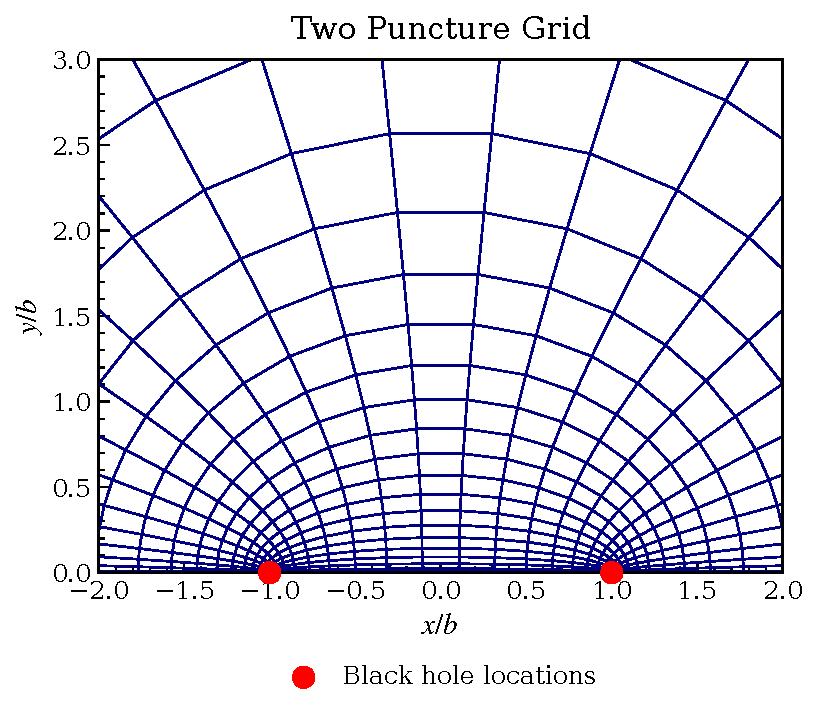
\includegraphics[width=0.75\textwidth]{Figures/twopunctures_grid.pdf}
    \caption{
    Example of the compactified TwoPunctures grid in a slice through the
    two punctures. The physical coordinates are shown in units of the
    half-separation $b$, with the black-hole punctures located at
    $x=\pm b$. The coordinate lines illustrate how the pseudo-spectral
    collocation points are distributed in the compactified domain before
    the resulting initial data are interpolated onto the evolution grid.
    The outer compactified boundary corresponds to spatial infinity and
    is outside the finite plotting window.
    }
    \label{fig:twopunctures_grid}
\end{figure}


\chapter{Computation of \texorpdfstring{$\Psi_4$}{Psi4}}
\label{sec:appx:wave_extraction}
\section{Wave Extraction}
\label{sec:app waveex}

This appendix summarizes the wave extraction procedure used for the gravitational, electromagnetic, dilaton, and axion radiation. The gravitational radiation is extracted from the Newman--Penrose scalar $\Psi_4$, while the electromagnetic radiation is extracted from the Maxwell Newman--Penrose scalars $\Phi_1$ and $\Phi_2$. We also define analogous outgoing scalar quantities for the dilaton and axion fields by projecting their gradients along an outgoing null direction.

\subsection{Null Tetrad and Spatial Triad}

The Newman--Penrose scalar $\Psi_4$ is defined by projecting the Weyl tensor onto a null tetrad:
\begin{equation}
    \Psi_4
    =
    C_{abcd} k^a \bar{m}^b k^c \bar{m}^d .
    \label{eq:app waveex psi4-def}
\end{equation}
Here $C_{abcd}$ is the Weyl tensor, and $k^a$ and $\bar{m}^a$ are elements of a null tetrad. The tetrad is constructed from the future directed unit normal $n^a$ to the spatial hypersurface and an orthonormal spatial triad $r^a$, $\theta^a$, and $\varphi^a$, which asymptotically approach the usual radial, polar, and azimuthal directions. We define
\begin{equation}
\begin{aligned}
    l^a
    &=
    \frac{1}{\sqrt{2}}\left(n^a+r^a\right),
    \\
    k^a
    &=
    \frac{1}{\sqrt{2}}\left(n^a r^a\right),
    \\
    m^a
    &=
    \frac{1}{\sqrt{2}}\left(\theta^a+i\varphi^a\right),
    \\
    \bar{m}^a
    &=
    \frac{1}{\sqrt{2}}\left(\theta^a i\varphi^a\right).
\end{aligned}
\label{eq:app waveex null tetrad}
\end{equation}
With metric signature $(-,+,+,+)$, these vectors satisfy
\begin{equation}
    l^a k_a = -1,
    \qquad
    m^a \bar{m}_a = 1,
\end{equation}
with all other tetrad inner products vanishing. In this appendix, $l^a$ denotes the null tetrad vector, while $\ell$ is reserved for the spherical harmonic mode index.

In practice, the spatial triad is constructed from coordinate vectors that approach the spherical coordinate basis vectors in the wave zone. We begin with
\begin{equation}
\begin{aligned}
    u^a &= (0,x,y,z),
    \\
    v^a &= (0,xz,yz,-x^2-y^2),
    \\
    w^a &= (0,-y,x,0).
\end{aligned}
\end{equation}
Using the spatial metric $\gamma_{ij}$, we define the spatial inner product
\begin{equation}
    \langle u,v\rangle
    =
    \gamma_{ij}u^i v^j
\end{equation}
and the associated norm
\begin{equation}
    |u|
    =
    \sqrt{\langle u,u\rangle}.
\end{equation}
The orthonormal triad is then obtained by Gram--Schmidt orthonormalization:
\begin{equation}
\begin{aligned}
    r^a
    &=
    \frac{u^a}{|u|},
    \\[0.5em]
    \theta^a
    &=
    \frac{
        v^a-\langle r,v\rangle r^a
    }{
        \left|v-\langle r,v\rangle r\right|
    },
    \\[0.5em]
    \varphi^a
    &=
    \frac{
        w^a
        -\langle r,w\rangle r^a
        -\langle \theta,w\rangle \theta^a
    }{
        \left|
        w
        -\langle r,w\rangle r
        -\langle \theta,w\rangle \theta
        \right|
    }.
\end{aligned}
\label{eq:app waveex spatial triad}
\end{equation}

\subsection{Gravitational Radiation}

The Weyl tensor is the trace free part of the spacetime curvature. In four dimensions, the Riemann tensor has twenty independent components. Ten of these are determined by the Ricci tensor, while the remaining ten are contained in the Weyl tensor. The Weyl tensor therefore captures the part of the curvature associated with tidal and radiative degrees of freedom.

In $n$ spacetime dimensions, with $n\geq 4$, the Weyl tensor is
\begin{equation}
\begin{aligned}
    C_{abcd}
    &=
    R_{abcd}
    +
    \frac{1}{n-2}
    \left(
        g_{ad} R_{cb}
        +
        g_{bc} R_{da}
        -
        g_{ac} R_{db}
        -
        g_{bd} R_{ca}
    \right)
    \\
    &\quad
    +
    \frac{1}{(n-1)(n-2)}
    \left(
        g_{ac}g_{db}
        -
        g_{ad}g_{cb}
    \right)R .
\end{aligned}
\label{eq:app waveex weyl nd}
\end{equation}
In four dimensions, this reduces to
\begin{equation}
\begin{aligned}
    C_{abcd}
    &=
    R_{abcd}
    +
    \frac{1}{2}
    \left(
        g_{ad} R_{cb}
        +
        g_{bc} R_{da}
        -
        g_{ac} R_{db}
        -
        g_{bd} R_{ca}
    \right)
    \\
    &\quad
    +
    \frac{1}{6}
    \left(
        g_{ac}g_{db}
        -
        g_{ad}g_{cb}
    \right)R .
\end{aligned}
\label{eq:app waveex weyl-4d}
\end{equation}
The Weyl tensor has the same index symmetries as the Riemann tensor:
\begin{equation}
    C_{abcd}
    =
    -C_{abdc}
    =
    -C_{bacd}
    =
    C_{cdab},
\end{equation}
together with the cyclic identity
\begin{equation}
    C_{abcd}
    +
    C_{adbc}
    +
    C_{acdb}
    =
    0 .
\end{equation}

At future null infinity, and for an appropriate outgoing tetrad, $\Psi_4$ encodes the outgoing gravitational radiation. With the convention used here, the complex strain
\begin{equation}
    h
    =
    h_+
    -
    i h_\times
\end{equation}
is related to $\Psi_4$ by
\begin{equation}
    \Psi_4
    =
    \ddot{h}_+
    -
    i\ddot{h}_\times
    =
    \ddot{h},
    \label{eq:app waveex psi4-strain}
\end{equation}
up to the overall sign convention chosen for the null tetrad. Therefore, the strain may be obtained by integrating $\Psi_4$ twice in time:
\begin{equation}
    h(t)
    =
    \int^t dt'
    \int^{t'} dt''\,
    \Psi_4(t'') .
    \label{eq:app waveex strain integral}
\end{equation}
In practice, this integration must be performed carefully because direct time domain integration can introduce secular drifts. Frequency domain methods, including fixed frequency integration, are often used to control low frequency numerical artifacts.

\subsection{Electromagnetic, Dilaton, and Axion Radiation}

The outgoing electromagnetic radiation is extracted using Newman--Penrose scalars associated with the Maxwell tensor \cite{Newman1962,Zilhao2014}. We define
\begin{align}
    \Phi_1
    &=
    \frac{1}{2}
    F_{ab}
    \left(
        l^a k^b
        +
        \bar{m}^a m^b
    \right),
    \label{eq:app waveex phi1-def}
    \\
    \Phi_2
    &=
    F_{ab}\bar{m}^a k^b .
    \label{eq:app waveex phi2-def}
\end{align}
At large radius, $\Phi_2$ represents the outgoing radiative electromagnetic degree of freedom.

We define analogous outgoing scalar quantities for the dilaton and axion fields by projecting their gradients along the outgoing null direction:
\begin{equation}
    \mathcal{D}
    =
    l^a\nabla_a\phi,
    \qquad
    \mathcal{A}
    =
    l^a\nabla_a\kappa .
    \label{eq:app waveex scalar radiation}
\end{equation}
Here $\mathcal{D}$ and $\mathcal{A}$ denote the extracted dilaton and axion radiation variables, respectively.

\subsection{Multipolar Decomposition}


\subsection{Relation to the \texorpdfstring{$3+1$}{3+1} Variables}

In numerical relativity, $\Psi_4$ is computed from quantities defined on spatial hypersurfaces. The spacetime curvature entering the Weyl tensor can therefore be related to the spatial metric $\gamma_{ij}$, the extrinsic curvature $K_{ij}$, and their derivatives using the Gauss--Codazzi relations. Schematically,
\begin{equation}
    \gamma^a{}_{i}
    \gamma^b{}_{j}
    \gamma^c{}_{k}
    \gamma^d{}_{l}
    {}^{(4)}R_{abcd}
    =
    {}^{(3)}R_{ijkl}
    +
    K_{ik}K_{jl}
    -
    K_{il}K_{jk},
    \label{eq:app waveex gauss}
\end{equation}
\begin{equation}
    \gamma^a{}_{i}
    \gamma^b{}_{j}
    \gamma^c{}_{k}
    n^d
    {}^{(4)}R_{abcd}
    =
    D_j K_{ik}
    -
    D_i K_{jk},
    \label{eq:app waveex codazzi}
\end{equation}
and
\begin{equation}
    \gamma^a{}_{i}
    \gamma^b{}_{j}
    n^c n^d
    {}^{(4)}R_{acbd}
    =
    \mathcal{L}_n K_{ij}
    +
    K_{ik}K^k{}_{j}
    +
    \frac{1}{\alpha}D_iD_j\alpha .
    \label{eq:app waveex ricci}
\end{equation}
These identities allow the spacetime curvature appearing in Eq.~\eqref{eq:app waveex psi4-def} to be expressed in terms of $3+1$ quantities on each slice.

After substituting the Gauss--Codazzi relations, $\Psi_4$ can be written in terms of spatial curvature and extrinsic curvature quantities. A common schematic form is
\begin{equation}
\begin{aligned}
    \Psi_4
    &=
    \left(
        {}^{(3)}R_{bd}
        +
        K K_{bd}
        -
        K_{bc}K^c{}_{d}
    \right)
    \bar{m}^b \bar{m}^d
    \\
    &\quad
    +
    \left(
        D_c K_{bd}
        -
        D_d K_{bc}
    \right)
    r^c \bar{m}^b \bar{m}^d ,
\end{aligned}
\label{eq:app waveex psi4-3plus1}
\end{equation}
where the precise signs depend on the conventions used for the Riemann tensor, the extrinsic curvature, and the null tetrad. In non vacuum evolutions, matter terms may also enter when the curvature is rewritten using the field equations. The important point is that $\Psi_4$ can be evaluated from the spatial geometry, the extrinsic curvature, and their derivatives on each time slice.

For BSSN type formulations, the extrinsic curvature is decomposed as
\begin{equation}
    K_{ij}
    =
    \chi^{-1}
    \left(
        \tilde{A}_{ij}
        +
        \frac{1}{3}\tilde{\gamma}_{ij}K
    \right),
    \label{eq:app waveex bssn kij}
\end{equation}
where $\tilde{\gamma}_{ij}$ is the conformal spatial metric, $\tilde{A}_{ij}$ is the trace free conformal extrinsic curvature, $K$ is the trace of the extrinsic curvature, and $\chi$ is the conformal factor used in the evolution system. Equivalently, if $\gamma_{ij}=e^{4\phi}\tilde{\gamma}_{ij}$, then $\chi=e^{-4\phi}$.

The resulting expressions for the real and imaginary parts of $\Psi_4$ in terms of BSSN variables are lengthy. They are therefore evaluated directly in the code using the evolved variables and their spatial derivatives. Symbolically, one may write
\begin{equation}
    \Psi_4
    =
    \mathrm{Re}(\Psi_4)
    +
    i\,\mathrm{Im}(\Psi_4),
\end{equation}
where the real and imaginary parts are obtained by projecting the curvature and extrinsic curvature terms onto the complex dyad formed from $m^a$ and $\bar{m}^a$.

\subsection{Waveform Mismatch}

To quantify the similarity between two gravitational waveforms, we compute a mismatch. A purely numerical comparison measures the waveform difference directly, while a detector based comparison weights the difference by the noise curve of a particular detector.

For two complex waveforms $h_1(t)$ and $h_2(t)$, a simple normalized overlap is
\begin{equation}
    \mathcal{O}
    =
    \frac{
        \left|
        \langle h_1,h_2\rangle
        \right|
    }{
        \sqrt{
            \langle h_1,h_1\rangle
            \langle h_2,h_2\rangle
        }
    },
\end{equation}
where a simple time domain inner product is
\begin{equation}
    \langle h_1,h_2\rangle
    =
    \int_{t_1}^{t_2}
    h_1(t)h_2^*(t)\,dt .
    \label{eq:app waveex time inner product}
\end{equation}
The mismatch is then
\begin{equation}
    \mathcal{M}
    =
    1-\mathcal{O}
\end{equation}
In practice, the overlap is maximized over relative time and phase shifts:
\begin{equation}
    \mathcal{M}
    =
    1
    -
    \max_{\Delta t,\Delta\phi}
    \frac{
        \left|
        \left\langle
            h_1,
            h_2^{\Delta t,\Delta\phi}
        \right\rangle
        \right|
    }{
        \sqrt{
            \langle h_1,h_1\rangle
            \langle h_2,h_2\rangle
        }
    } .
    \label{eq:app waveex mismatch maximized}
\end{equation}
Here $h_2^{\Delta t,\Delta\phi}$ denotes the waveform $h_2$ shifted in time by $\Delta t$ and rotated by an overall phase $\Delta\phi$. This maximization removes trivial offsets in arrival time and phase, leaving a measure of the physical disagreement between the waveform shapes. A smaller mismatch indicates better agreement.

For detector weighted comparisons, one instead uses the frequency domain inner product
\begin{equation}
    \left(h_1,h_2\right)
    =
    4\,\mathrm{Re}
    \int_{f_{\min}}^{f_{\max}}
    \frac{
        \tilde{h}_1(f)\tilde{h}_2^*(f)
    }{
        S_n(f)
    }\,df ,
    \label{eq:app waveex noise inner product}
\end{equation}
where $\tilde{h}(f)$ is the Fourier transform of $h(t)$ and $S_n(f)$ is the one sided detector noise power spectral density. The detector weighted overlap is
\begin{equation}
    \mathcal{O}
    =
    \frac{
        \left(h_1,h_2\right)
    }{
        \sqrt{
            \left(h_1,h_1\right)
            \left(h_2,h_2\right)
        }
    },
    \label{eq:app waveex noise overlap}
\end{equation}
again maximized over relative time and phase shifts. The corresponding mismatch is
\begin{equation}
    \mathcal{M}
    =
    1
    -
    \max_{\Delta t,\Delta\phi}
    \mathcal{O}.
    \label{eq:app waveex noise mismatch}
\end{equation}
This detector weighted mismatch is the more relevant quantity when assessing whether two waveforms could be distinguished by a particular gravitational wave detector.

\chapter{Dendro Notes}
\section{Wavelet Adaptive Mesh Refinement}
\label{sec:wamr}

Dendro employs wavelet adaptive mesh refinement (WAMR) to construct a sparse representation of the evolved fields while maintaining resolution in regions where the solution contains significant spatial structure. The basic idea is to represent the computational domain using a hierarchy of nested dyadic grids. In one spatial dimension, these grids may be written as
\begin{equation}
    V_j
    =
    \left\{
        x^{j,k}
        =
        2^{-j} k\,\Delta x
    \right\},
\end{equation}
where $j$ denotes the refinement level, $k$ indexes the points on that level, and $\Delta x$ is the spacing on the coarsest grid. If the physical domain has length $L$ and the base grid $V_0$ contains $N+1$ points, then
\begin{equation}
    \Delta x = \frac{L}{N}.
\end{equation}
The grids are nested, so points present on a coarse level also appear on all finer levels. In particular, points with even index on level $j+1$ coincide with points on level $j$,
\begin{equation}
    x^{j+1,2k} = x^{j,k}.
\end{equation}
The multidimensional AMR hierarchy used in the simulations is built from the same dyadic refinement idea.

Figure~\ref{fig:wamr grid hierarchy} illustrates this nested structure in one dimension. The black points denote grid points inherited from coarser levels, while the red points denote the additional points introduced at each refinement level. These additional points form the detail spaces $W_j$, which contain the information added when passing from level $j-1$ to level $j$.

\begin{figure}[t]
\centering
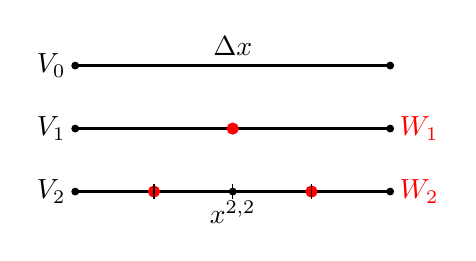
\begin{tikzpicture}[scale=1]
    % V0 line
    \draw[thick] (0,0) -- (4,0);
    \node[left] at (0,0) {$V_0$};
    \node[above] at (2,0) {$\Delta x$};

    % Endpoints for V0
    \filldraw (0,0) circle (1.2pt);
    \filldraw (4,0) circle (1.2pt);

    % V1 line
    \draw[thick] (0,-0.8) -- (4,-0.8);
    \node[left] at (0,-0.8) {$V_1$};
    \node[right, red] at (4,-0.8) {$W_1$};
    \filldraw (0,-0.8) circle (1.2pt);
    \filldraw[red] (2,-0.8) circle (2pt);
    \filldraw (4,-0.8) circle (1.2pt);

    % V2 line
    \draw[thick] (0,-1.6) -- (4,-1.6);
    \node[left] at (0,-1.6) {$V_2$};
    \node[right, red] at (4,-1.6) {$W_2$};
    \filldraw (0,-1.6) circle (1.2pt);
    \filldraw[red] (1,-1.6) circle (2pt);
    \filldraw (2,-1.6) circle (1.2pt);
    \filldraw[red] (3,-1.6) circle (2pt);
    \filldraw (4,-1.6) circle (1.2pt);
    \node[below] at (2,-1.6) {$x^{2,2}$};

    % Ticks
    \foreach \x in {1,2,3} {
        \draw (\x,-1.5) -- (\x,-1.7);
    }
\end{tikzpicture}
\caption{
Schematic illustration of the nested dyadic grids used in wavelet adaptive mesh refinement. Points present on coarser grids are retained on finer grids, while the red points indicate the additional degrees of freedom introduced at each refinement level. These additional points correspond to the detail spaces $W_j$.
}
\label{fig:wamr grid hierarchy}
\end{figure}

Let $u^{j,k}$ denote the value of a field $u$ at the grid point $x^{j,k}$. Since the grids are nested, values at points inherited from the previous level satisfy
\begin{equation}
    u^{j+1,2k}
    =
    u^{j,k}.
\end{equation}
The values at newly introduced points may be estimated by interpolation from the previous level,
\begin{equation}
    u^{j+1,2k+1}
    =
    \sum_m h^{j+1,2k+1}_{j,m}\,u^{j,m},
\end{equation}
where $h^{j+1,2k+1}_{j,m}$ are the interpolation weights. In practice only a small number of these coefficients are nonzero. For the fourth order interpolation used here, the interior interpolation stencil is
\begin{equation}
    u^{j+1,2k+1}
    =
    -\frac{1}{16}u^{j,k-1}
    +\frac{9}{16}u^{j,k}
    +\frac{9}{16}u^{j,k+1}
    -\frac{1}{16}u^{j,k+2}.
\end{equation}
Near physical boundaries the same interpolation idea is used, but the stencil is shifted so that it remains inside the domain, leading to modified one sided interpolation weights.

Equivalently, this interpolation can be described in terms of scaling functions. A basis function on level $j$ may be represented using basis functions on the finer level $j+1$ as
\begin{equation}
    \phi_{j,k}(x)
    =
    \sum_l c_l\,\phi_{j+1,l}(x),
\end{equation}
where the coefficients $c_l$ encode the interpolation stencil. For the fourth order stencil above, the corresponding nonzero two scale coefficients are
\begin{equation}
    c_l
    =
    \left\{
        \ldots,
        0,
        -\frac{1}{16},
        0,
        \frac{9}{16},
        1,
        \frac{9}{16},
        0,
        -\frac{1}{16},
        0,
        \ldots
    \right\}.
\end{equation}
Each basis function may be viewed as a scaled and translated copy of a single fundamental interpolating function,
\begin{equation}
    \phi_{j,k}(x)
    =
    \phi\!\left(\frac{2^j x}{\Delta x} - k\right).
\end{equation}

The nested nature of the grids introduces redundancy if basis functions are included for every point on every level. To avoid this, one introduces alternate grids $W_j$ for $j>0$, consisting only of the points that first appear at level $j$:
\begin{equation}
    W_j
    =
    \left\{
        x^{j,k} : x^{j,k}=2^{-j}k\Delta x,
        \quad k \ \mathrm{odd}
    \right\}.
\end{equation}
Thus the collection $\{V_0,W_1,W_2,\ldots\}$ represents each grid point exactly once. The corresponding index sets are
\begin{equation}
    S_0 = \{0,1,\ldots,N\},
    \qquad
    S_j = \{1,3,\ldots,2^jN-1\},
\end{equation}
where $S_0$ labels the base grid and $S_j$ labels the detail points on level $j$.

This nested basis construction allows the field to be represented by a coarse contribution together with corrections from the detail spaces. A field can be expanded as
\begin{equation}
    u(x)
    =
    \sum_{k \in S_0}
    u^{0,k}\,\phi_{0,k}(x)
    +
    \sum_{j=1}^{J}
    \sum_{k \in S_j}
    d^{j,k}\,\phi_{j,k}(x),
\end{equation}
where $u^{0,k}$ are the base level field values and $d^{j,k}$ are the wavelet coefficients. This is the interpolating wavelet representation of the field. The first term gives the coarse representation on the base grid, while the remaining terms give the corrections required at successively finer levels.

The wavelet coefficient at a detail point is computed by comparing the actual field value to the value predicted by interpolation from the previous refinement level,
\begin{equation}
    d^{j,k}
    =
    u^{j,k}
    -
    P\!\left(x^{j,k},j-1\right),
\end{equation}
where $P(x^{j,k},j-1)$ denotes the interpolated value obtained from level $j-1$. Thus, the coefficient $d^{j,k}$ measures the local interpolation error associated with omitting the point $x^{j,k}$. This transformation from point values to wavelet coefficients is the forward wavelet transformation. It can be inverted by reconstructing the field values from the base level values and the wavelet coefficients.

There are therefore two equivalent descriptions of the field on the multi level grid. The first is the point representation, given by the field values $\{u^{j,k}\}$. The second is the wavelet representation, given by the base values and wavelet coefficients,
\begin{equation}
    \{u^{0,k},d^{j,k}\}.
\end{equation}
The wavelet representation can be made sparse by discarding points whose wavelet coefficients are below a prescribed tolerance $\varepsilon$,
\begin{equation}
    |d^{j,k}| < \varepsilon .
\end{equation}
These discarded points are well approximated by interpolation from coarser levels. The retained points are called essential points, and all base level points are always retained. The field values on the essential points form the sparse point representation. For interpolating wavelets, thresholding the coefficients also provides an a priori control of the representation error, with constants determined by the interpolation basis.

In practice, refinement is controlled by the tolerance $\varepsilon$, and detail points are retained when, schematically,
\begin{equation}
    |d^{j,k}| > \varepsilon .
\end{equation}
This criterion provides an efficient adaptive representation: smooth regions of the solution are represented using relatively few points, while regions containing sharp gradients, wave propagation, or strong field structure are refined automatically.

In higher dimensions the construction is extended by taking tensor products of the one dimensional basis functions. In three spatial dimensions,
\begin{equation}
    \phi_{j,\mathbf{k}}(x,y,z)
    =
    \phi_{j,k_x}(x)
    \phi_{j,k_y}(y)
    \phi_{j,k_z}(z),
\end{equation}
where $\mathbf{k}=(k_x,k_y,k_z)$. Equivalently, interpolation can be performed directly in multiple dimensions. Depending on the location of the new point relative to the previous level, the interpolation stencil may involve $p$, $p^2$, or $p^3$ points, where $p$ is the one dimensional interpolation order. The wavelet coefficient is again computed as the difference between the actual field value and the value interpolated from the previous level.

The multidimensional wavelet expansion has the form
\begin{equation}
    u(x,y,z)
    =
    \sum_{\mathbf{k}}
    u^{0,\mathbf{k}}\,
    \phi_{0,\mathbf{k}}(x,y,z)
    +
    \sum_{j=1}^{J}
    \sum_{\mathbf{k}}
    d^{j,\mathbf{k}}\,
    \phi_{j,\mathbf{k}}(x,y,z).
\end{equation}
As in one dimension, sparse refinement is obtained by retaining only those points whose wavelet coefficients exceed the chosen tolerance. This produces an adaptive multi level grid that concentrates resolution where the evolved fields are not accurately represented by interpolation from coarser levels.

\section{Sobolev Informed Refinement}
\label{sec:sobolev amr}

In addition to the standard wavelet criterion, we also consider a Sobolev inspired modification of the refinement. The purpose of this modification is to make the refinement criterion sensitive not only to the local wavelet truncation estimate of a field, but also to local derivative content. This is useful in regions where the field itself may be relatively smooth in amplitude, while its gradients or curvature contain dynamically relevant structure.

For a given evolved variable $u$, the standard wavelet refinement indicator may be denoted by
\begin{equation}
    I_{\mathrm{W}}(u).
\end{equation}
This quantity represents the usual WAMR estimate based on the magnitude of the local wavelet coefficient. The Sobolev informed indicator augments this quantity by including contributions from first and second spatial derivatives. We use an indicator of the form
\begin{equation}
    I_{\mathrm{Sob}}(u)
    =
    \sqrt{
        I_{\mathrm{W}}(u)^2
        +
        w_1 I_{\nabla u}^2
        +
        w_2 I_{\nabla^2 u}^2
    },
    \label{eq:sobolev amr indicator}
\end{equation}
where $I_{\nabla u}$ is a local first derivative indicator, $I_{\nabla^2 u}$ is a local second derivative indicator, and $w_1$ and $w_2$ are user controlled weights. Any required normalization of the derivative indicators is absorbed into these weights. The first derivative term increases refinement in regions with large gradients, while the second derivative term increases refinement in regions with large curvature or rapidly changing gradients.

This refinement measure should be interpreted as a \emph{Sobolev inspired} or \emph{Sobolev weighted} WAMR indicator rather than as an exact discrete Sobolev norm. A true Sobolev norm is a global or integrated quantity involving a function and its derivatives. By contrast, Eq.~\eqref{eq:sobolev amr indicator} is a local AMR indicator designed to guide mesh refinement. Its role is to bias the adaptive mesh toward regions where derivative information suggests that additional resolution may be needed, while retaining the efficiency of the underlying wavelet based refinement algorithm.

We demonstrate this in action with code evolving Maxwell's equations. The following figures compare the baseline wavelet adaptive mesh refinement criterion with the Sobolev informed refinement criterion. These diagnostics compare both the constraint behavior of the two refinement strategies and the computational cost associated with the resulting adaptive meshes.

Figure~\ref{fig:sobolev amr mesh comparison} shows a representative side by side comparison of the adaptive mesh structure produced by the two refinement criteria. The Sobolev informed criterion modifies the local refinement indicator by including derivative information, which changes the distribution of refined regions relative to the baseline wavelet criterion.

\begin{figure}[t]
\centering
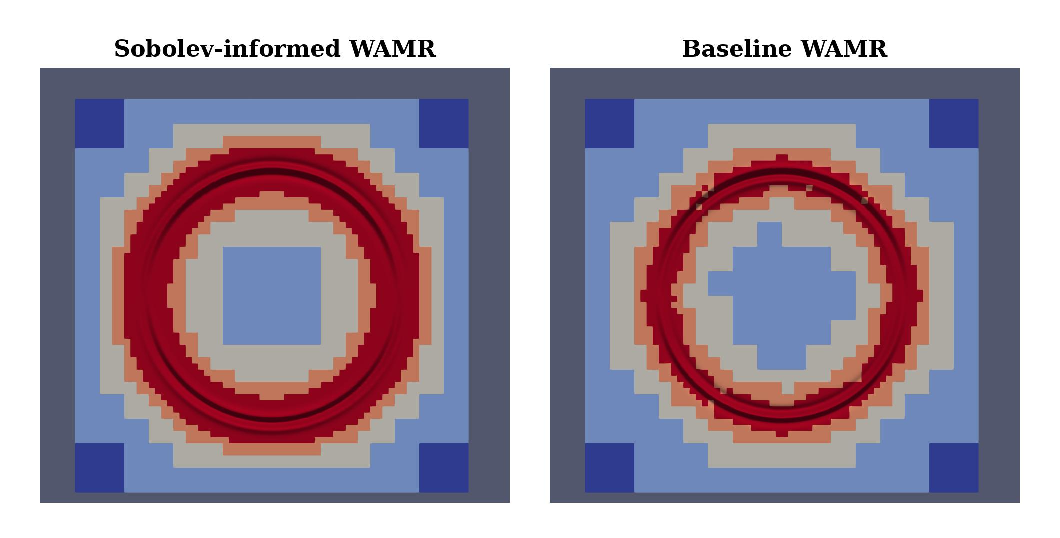
\includegraphics[width=0.85\textwidth]{Figures/Appendix/sobolev_wamr_labeled_side_by_side.pdf}
\caption{
Representative comparison of the adaptive mesh generated by the baseline wavelet AMR criterion and the Sobolev informed AMR criterion. The red areas represent areas of higher refinment the blue areas represent the areas with lower refinment. The Sobolev informed criterion includes derivative information in the refinement indicator, which changes where grid points are allocated. The oscillatory ring corresponds to the outward propagating dipole pulse. Notice that the sobolev inspired refinement produces a much more symmetric refinement. The Sobolev inspired criteria is more expensive but refines around the region of interest better.
}
\label{fig:sobolev amr mesh comparison}
\end{figure}

Figure~\ref{fig:sobolev amr constraints} shows the divergence constraints for the electric and vector potential fields. These quantities provide a direct measure of the constraint violation during the evolution. The comparison shows how the Sobolev informed refinement criterion affects the constraint preserving behavior of the evolution relative to the baseline wavelet criterion. Notice how much better the sobolev inspired does relative to the base case.

\begin{figure}[t]
\centering

\subfloat[$L_2$ norm of $\nabla_i E^i$.]{%
    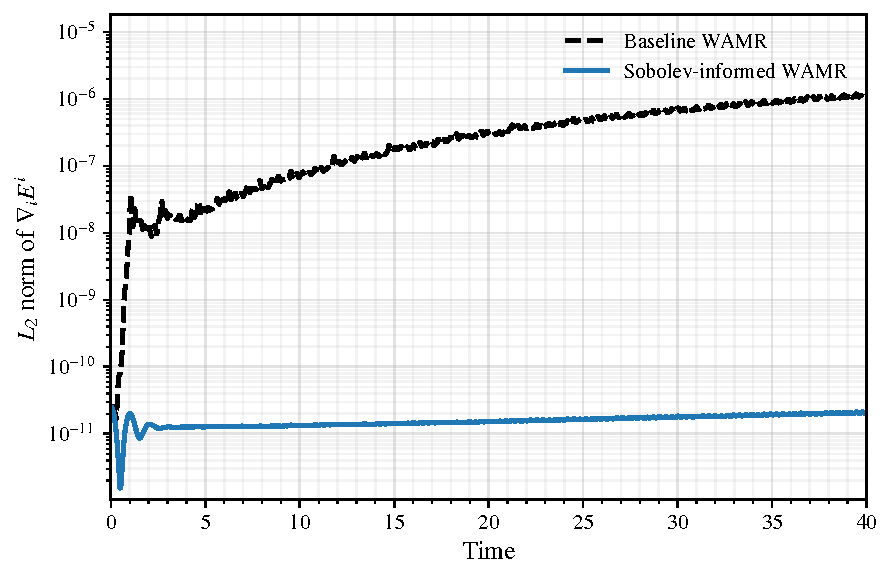
\includegraphics[width=0.48\textwidth]{Figures/Appendix/DivE_wavelet_tolerance_comparison.pdf}%
    \label{fig:sobolev amr dive}%
}
\hfill
\subfloat[$L_2$ norm of $\nabla_i A^i$.]{%
    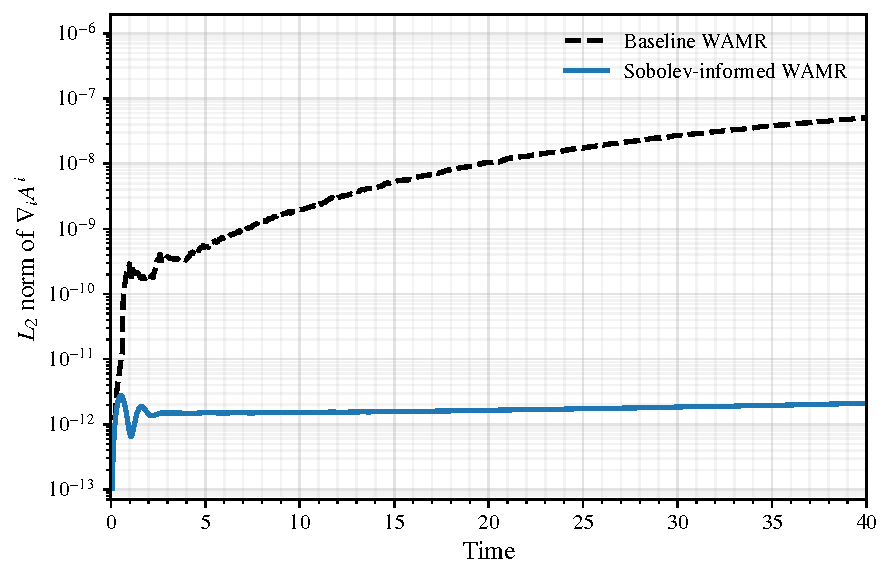
\includegraphics[width=0.48\textwidth]{Figures/Appendix/DivA_wavelet_tolerance_comparison.pdf}%
    \label{fig:sobolev amr diva}%
}

\caption{
Constraints for the baseline wavelet AMR and Sobolev informed AMR refinement criteria. The left panel shows the $L_2$ norm of the electric field divergence constraint, while the right panel shows the corresponding divergence for the vector potential. These quantities are used to assess whether the modified refinement indicator improves or degrades the constraint behavior of the evolution.
}
\label{fig:sobolev amr constraints}
\end{figure}

Figure~\ref{fig:sobolev amr efficiency} compares the number of active mesh points and a measure of the grid efficiency. The number of active mesh points, $N_{\mathrm{mesh}}$, measures the size of the adaptive grid and is therefore a proxy for the computational cost of the evolution. A refinement strategy that achieves comparable or smaller constraint violations using fewer mesh points is more efficient.

To quantify this tradeoff, we define the grid efficency as:
\begin{equation}
    \eta
    =
    \frac{1}{C_{\mathrm{tot}} N_{\mathrm{mesh}}^2},
    \label{eq:sobolev amr grid efficiency}
\end{equation}
where $C_{\mathrm{tot}}$ is the total constraint measure and $N_{\mathrm{mesh}}$ is the number of active mesh points. In this work, the total constraint measure is constructed from the divergence constraints as
\begin{equation}
    C_{\mathrm{tot}}
    =
    C_{\nabla E}
    +
    C_{\nabla A},
    \label{eq:sobolev amr total constraint}
\end{equation}
where $C_{\nabla E}$ and $C_{\nabla A}$ denote the $L_2$ norms of the corresponding divergences. With this definition, larger values of $\eta$ indicate that a simulation achieves smaller constraint violation for a given mesh size. The factor of $N_{\mathrm{mesh}}^2$ penalizes simulations that reduce the constraint violation only by using substantially more grid points.

\begin{figure}[t]
\centering

\subfloat[Number of active mesh points.]{%
    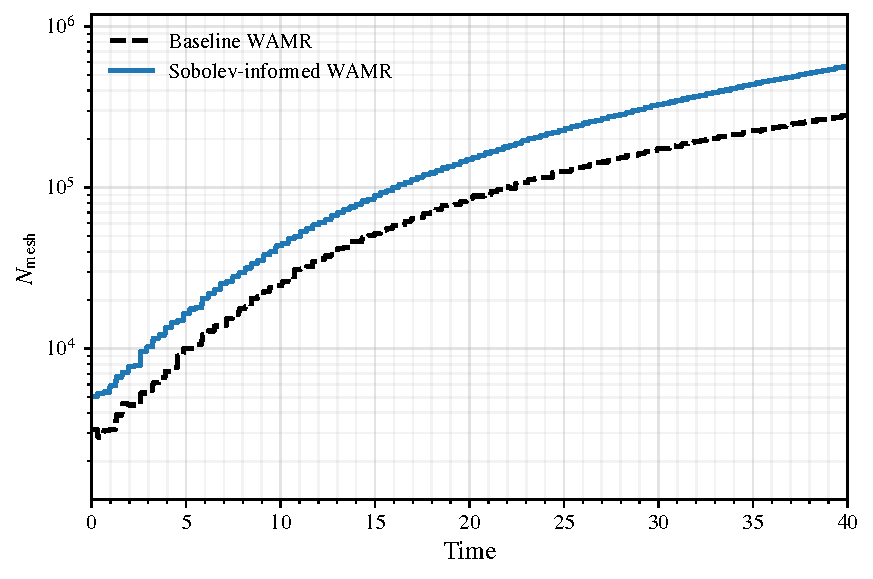
\includegraphics[width=0.48\textwidth]{Figures/Appendix/mesh_size_wavelet_tolerance_comparison.pdf}%
    \label{fig:sobolev amr mesh size}%
}
\hfill
\subfloat[Grid efficiency.]{%
    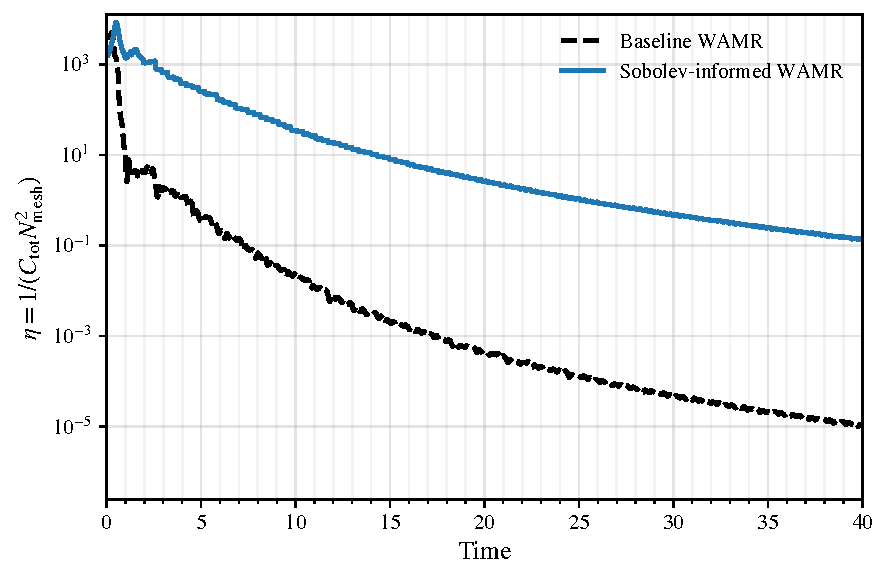
\includegraphics[width=0.48\textwidth]{Figures/Appendix/grid_efficiency_wavelet_tolerance_comparison.pdf}%
    \label{fig:sobolev amr grid efficiency}%
}

\caption{
Mesh size and grid efficiency for the baseline wavelet AMR and Sobolev informed AMR refinement criteria. The left panel shows the number of active mesh points $N_{\mathrm{mesh}}$, which serves as a proxy for computational cost. The right panel shows $\eta = 1/(C_{\mathrm{tot}}N_{\mathrm{mesh}}^2)$. Larger values of $\eta$ indicate smaller constraint violation for a given mesh size, and therefore a more efficient use of grid points.
}
\label{fig:sobolev amr efficiency}
\end{figure}

\chapter{CFD Notes}
\section{CFD Stability Tests}

In addition to the eigenvalue stability analysis discussed in the main
chapter, we performed numerical stability tests of the compact operators
using both Maxwell's equations and the BSSN equations. Representative
results from these tests are presented below.

For the Maxwell test, the computational domain extends over
$x,y,z\in[-20,20]$. We use the same initial data and numerical parameters
described in the computational fluid dynamics chapter and perform the
evolution on the corresponding low resolution uniform grid. The numerical
error remains bounded throughout the evolution and decreases cleanly after
the initial electromagnetic pulse propagates across the domain. We find no
evidence of growing numerical modes for any of the operators shown in
Fig.~\ref{fig:EM_all_operator_errors}.

\begin{figure}[htbp]
    \centering
    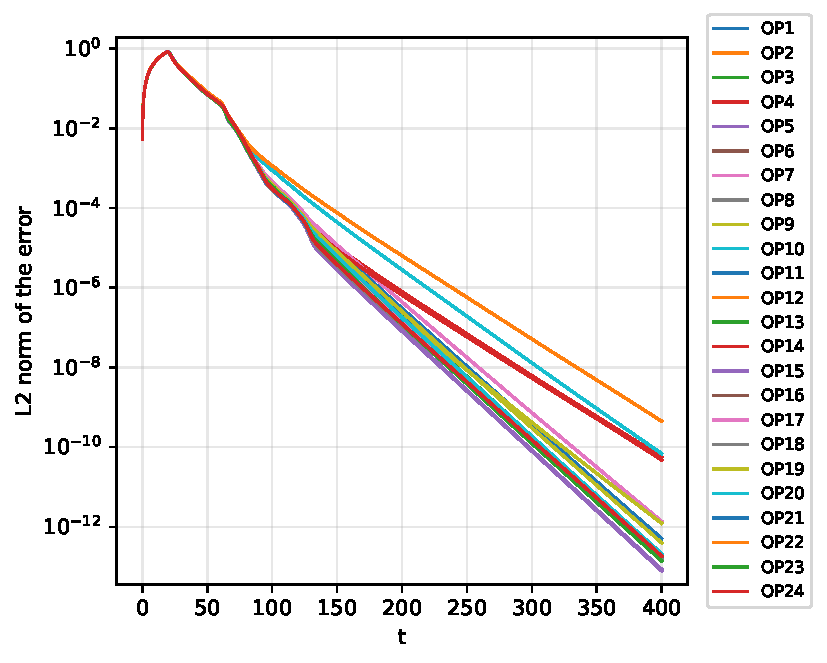
\includegraphics[width=0.9\textwidth]
    {Figures/Appendix/EM_all_operator_errors.pdf}
    \caption{
    Evolution of the numerical errors for the finite difference operators
    applied to the Maxwell test problem. The simulations use a uniform grid
    on the domain $x,y,z\in[-20,20]$ with the same initial data and numerical
    parameters used in the Maxwell tests presented in the main text. The
    errors remain bounded and decay cleanly as the electromagnetic pulse
    propagates out of the computational domain, with no evidence of a
    numerical instability.
    }
    \label{fig:EM_all_operator_errors}
\end{figure}

We also test the operators by evolving Teukolsky wave initial data with the
full BSSN equations. The computational domain extends over
$x,y,z\in[-40,40]$. We use outgoing, even parity initial data in the
quadrupolar mode $(\ell,m)=(2,0)$ with amplitude
$\mathcal{A}=10^{-2}$. The initial perturbation is centered at
$r_0=20$ and is constructed from a compactly supported $C^k$ radial
profile with $k=6$ and half width $w=2$.

The simulations use the same remaining numerical parameters as the
Teukolsky wave tests described in the main chapter. We evolve the solution
for more than ten characteristic crossing times in order to identify any
slowly growing unstable modes. As shown in
Fig.~\ref{fig:all_momentum_x_errors}, the momentum constraint errors remain
bounded and decay to small values throughout the evolution. This smooth
long term behavior provides further evidence that the compact operators
remain stable when applied to the BSSN system.

\begin{figure}[htbp]
    \centering
    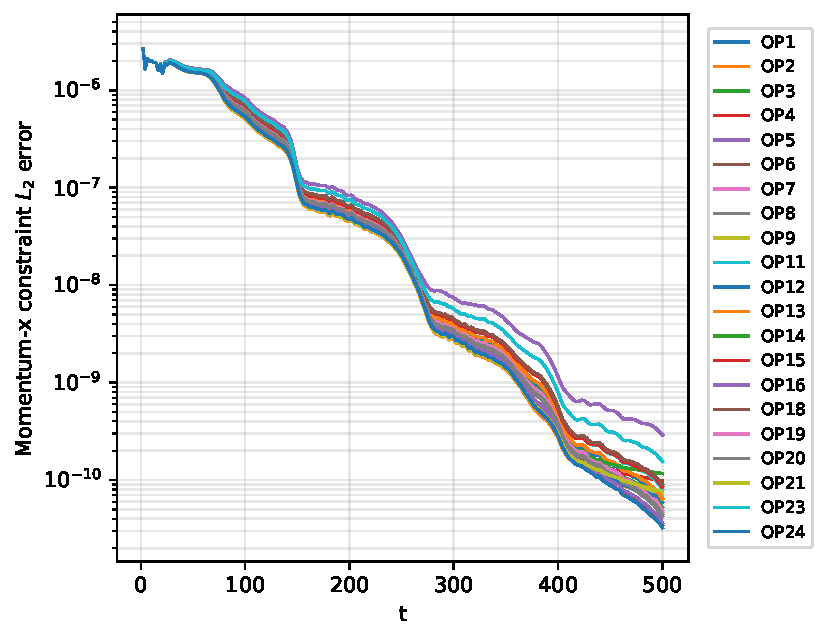
\includegraphics[width=0.9\textwidth]
    {Figures/Appendix/all_momentum_x_errors.pdf}
    \caption{
    Evolution of the momentum constraint error during the Teukolsky wave
    stability test for the finite difference operators considered in this
    work. The computational domain is $x,y,z\in[-40,40]$, and the initial
    data describe an outgoing, even parity Teukolsky wave in the
    $(\ell,m)=(2,0)$ mode with amplitude $\mathcal{A}=10^{-2}$.
    The initial perturbation is centered at $r_0=20$ and uses a compactly
    supported $C^k$ radial profile with $k=6$ and half width $w=2$.
    The errors remain bounded and decay smoothly to small values over more
    than ten characteristic crossing times, with no evidence of a growing
    numerical instability.
    }
    \label{fig:all_momentum_x_errors}
\end{figure}


\section{Black Hole Merger Tests with CFDs}
\label{sec:black_hole_merger_tests}

We also compare the performance of compact and explicit finite difference
operators in an inspiraling equal mass binary black hole merger. The binary
has mass ratio $q=1$, an initial separation of $8M$, and quasicircular initial
data.

We compare evolutions using fourth-order compact and explicit finite-difference operators with a finest resolution of (h=0.0325) against a more highly resolved sixth-order explicit finite-difference evolution with a finest resolution of (h=0.016).

The resulting gravitational waveforms are shown in
Figs.~\ref{fig:bbh_waveforms_overlay} and
\ref{fig:bbh_waveforms_peak_aligned_subtraction}. The fourth order explicit
evolution is underresolved, which produces a noticeable shift in the merger
time. Differences also remain after aligning the waveforms at their peaks.

These results show that the compact operators can outperform explicit
operators of the same nominal order in a fully nonlinear numerical relativity
simulation. In particular, the compact evolution more closely follows the
higher resolution sixth order explicit reference waveform. Further tests are
ongoing to determine how robust these improvements remain across different
resolutions, binary parameters, and longer inspiral evolutions.

\begin{figure}[t]
    \centering
    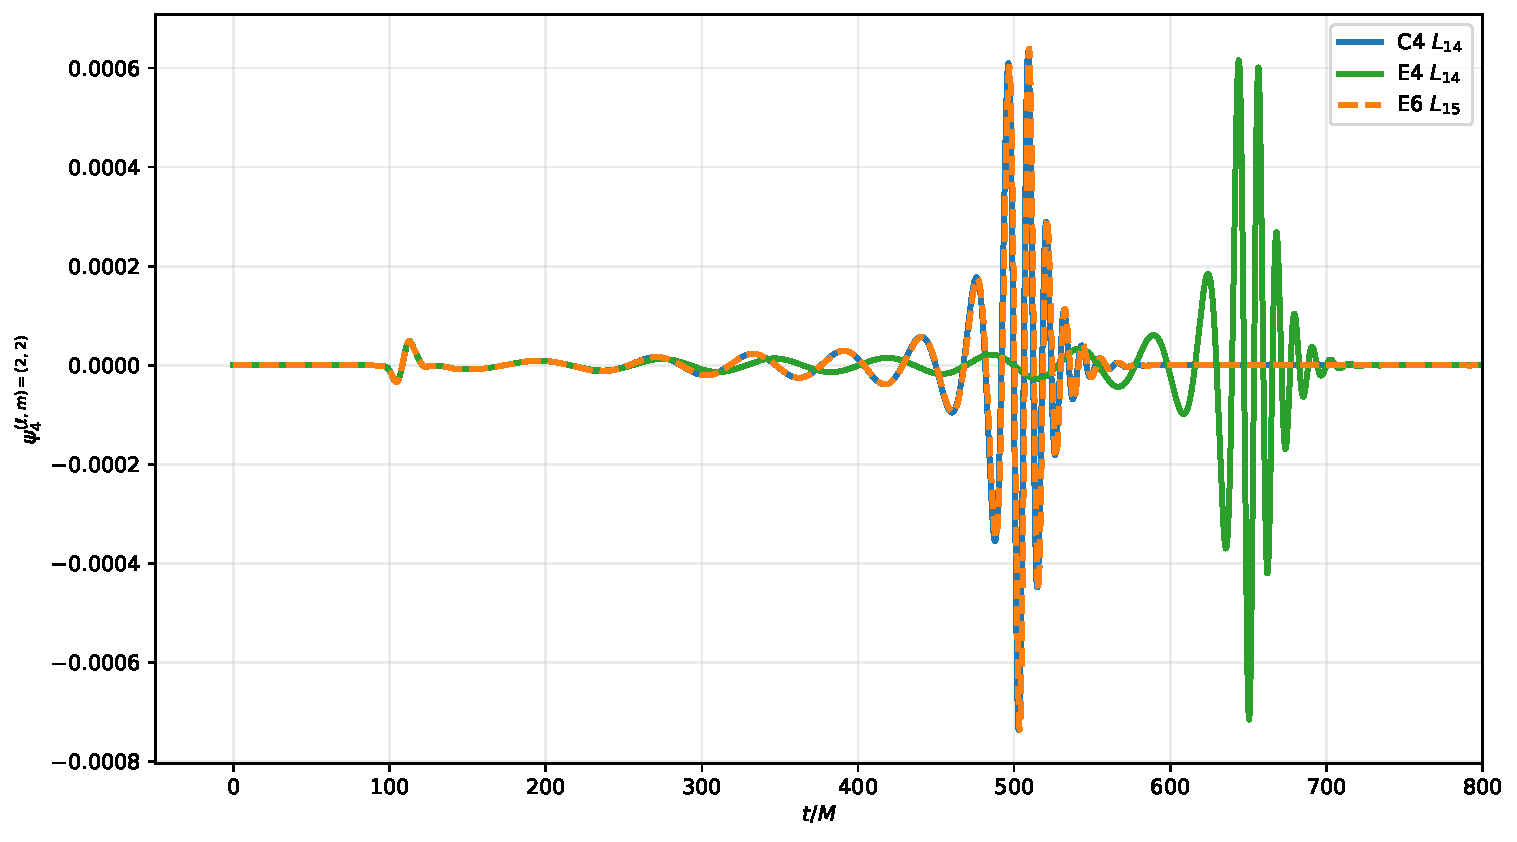
\includegraphics[width=\textwidth]
        {Figures/Appendix/waveforms_overlay.pdf}
    \caption{
    Comparison of the gravitational waveforms from the equal mass binary
    black hole merger evolved with compact and explicit finite difference
    operators. The binary has mass ratio $q=1$, initial separation $8M$, and
    quasicircular initial data. A more highly resolved sixth order explicit
    evolution is included as a reference. The underresolved fourth order
    explicit evolution shows a noticeable shift in merger time, while the
    compact evolution remains closer to the reference waveform.
    }
    \label{fig:bbh_waveforms_overlay}
\end{figure}

\begin{figure}[t]
    \centering
    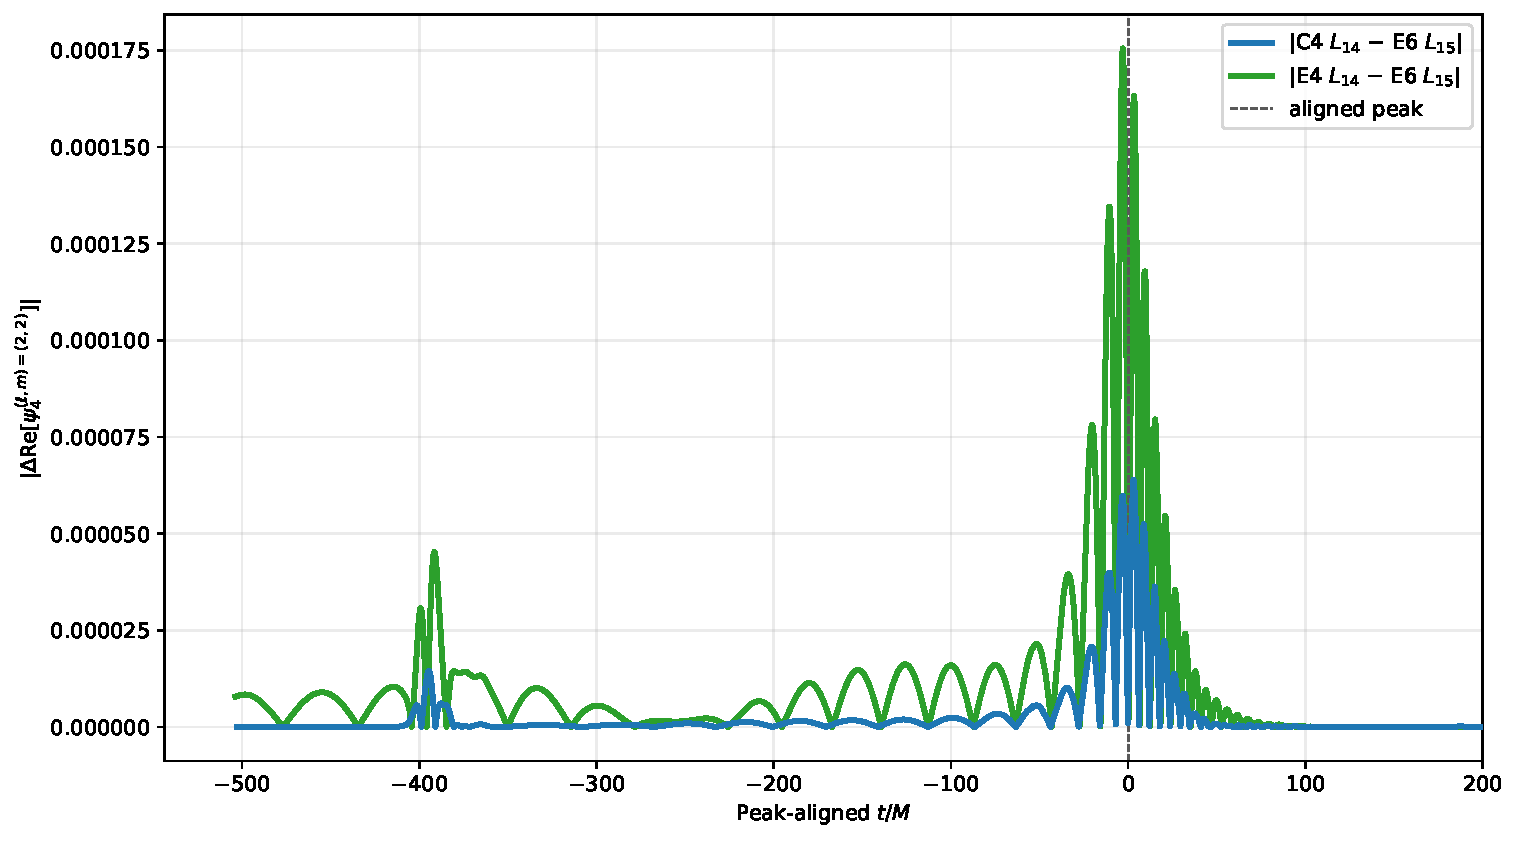
\includegraphics[width=\textwidth]
        {Figures/Appendix/waveforms_peak_aligned_subtraction.pdf}
    \caption{
    Differences between the peak aligned gravitational waveforms from the
    compact and explicit finite difference evolutions and the more highly
    resolved sixth order explicit reference waveform. Peak alignment removes
    the leading merger time offset and highlights differences in waveform
    amplitude and phase. The compact evolution agrees more closely with the
    reference waveform than the underresolved fourth order explicit
    evolution.
    }
    \label{fig:bbh_waveforms_peak_aligned_subtraction}
\end{figure}


\chapter{EMDA Code Setup on MaryLou}

\section{Building \texttt{emda-gr}}
To build \texttt{emda-gr}, the following external packages are required:
\begin{itemize}
\item \textbf{C/C++11 or higher} (tested with GNU and Intel compilers)
\item \textbf{MPI implementation} (tested with \texttt{MVAPICH2}, \texttt{OpenMPI}, and Intel MPI)
\item \textbf{BLAS/LAPACK} (tested with \texttt{OpenBLAS} and Intel MKL)
\item \textbf{GSL} (GNU Scientific Library); set \texttt{GSL\_ROOT\_DIR} in \texttt{CMake} to enable automatic detection
\end{itemize}

On MaryLou, the recommended module environment is:

\begin{verbatim}
andrewc0@login03:$ ml
Currently Loaded Modules:

1. gcc/14.1
2. python/3.12
3. cmake/3.28
4. gcc-runtime/13.2.0-g4hc7ev
5. eigen/3.4.0-6kqviac
6. openmpi5-GR
7. gsl-GR
8. mkl-GR
9. rclone/1.65.2-tyg4lvy
   \end{verbatim}

To ensure that these dependencies are always available, it is convenient to load
them automatically in your shell configuration. Open your
\texttt{\textasciitilde/.bash\_profile}:

\begin{verbatim}
vim ~/.bash_profile
\end{verbatim}

An example \texttt{.bash\_profile} is shown below. Additional customizations may
be added as needed.

\begin{verbatim}

# --- Modules ---

module purge
module use /grphome/grp_GR/.modulefiles
module load gcc/14.1 python/3.12 cmake/3.28 eigen/3.4.0-6kqviac
module load openmpi5-GR gsl-GR mkl-GR rclone

export HCOLL_DIR=/vapps/rhel9/x86_64/HPC-X/hpcx-v2.19-gcc-inbox-redhat9-cuda12-x86_64/hcoll/lib
export LD_LIBRARY_PATH="${HCOLL_DIR}:${LD_LIBRARY_PATH:-}"

# --- GSL ---

export GSL_DIR=/grphome/grp_GR/apps/gsl-2.8
export GSL_ROOT_DIR=/grphome/grp_GR/apps/gsl-2.8
export LD_LIBRARY_PATH="${GSL_DIR}/lib:${LD_LIBRARY_PATH:-}"

# --- MKL ---

if [ -n "${MKLROOT:-}" ] && [ -d "${MKLROOT}/lib/intel64" ]; then
export LD_LIBRARY_PATH="${MKLROOT}/lib/intel64:${LD_LIBRARY_PATH:-}"
fi

# --- GCC 14 runtime: libstdc++ and libgcc_s ---

# Required to avoid GLIBCXX and CXXABI runtime errors.

if command -v g++ >/dev/null 2>&1; then
GCC_LIBDIR="$(dirname "$(g++ -print-file-name=libstdc++.so.6)")"
GCC_GCCLIBDIR="$(dirname "$(g++ -print-file-name=libgcc_s.so.1)")"

if [ -d "$GCC_LIBDIR" ]; then
export LD_LIBRARY_PATH="$GCC_LIBDIR:${LD_LIBRARY_PATH:-}"
fi
if [ -d "$GCC_GCCLIBDIR" ]; then
export LD_LIBRARY_PATH="$GCC_GCCLIBDIR:${LD_LIBRARY_PATH:-}"
fi
fi

# --- History settings ---

HISTSIZE=1000000
HISTFILESIZE=2000000
HISTCONTROL=ignoredups:erasedups
HISTIGNORE="ls:bg:fg:history"
shopt -s histappend

# Save history after every command.

PROMPT_COMMAND="history -a; history -c; history -r; $PROMPT_COMMAND"
\end{verbatim}

After reloading the shell, verify that the modules have been loaded correctly:

\begin{verbatim}
ml
\end{verbatim}

The output should match the module list shown above.

\section{Building the Solver}

First, clone the EMDA repository. Create a project directory if desired, then run:

\begin{verbatim}
git clone [git@github.com](mailto:git@github.com):dfvankomen/emda-gr.git
cd emda-gr
\end{verbatim}

CMake will automatically fetch \texttt{dendrolib} during configuration.

Create and enter a build directory:

\begin{verbatim}
mkdir build
cd build
\end{verbatim}

Configure the project using:

\begin{verbatim}
ccmake ..
\end{verbatim}

CMake will locate the required libraries and open an interactive configuration
interface. The main settings that may need to be adjusted are the system of
equations and the target CPU architecture.

The available equation systems include EMDA, EMD, and EMGR. For a first test
run, choose the EMDA system.

The CPU architecture should match the compute nodes on which the job will run.
On MaryLou, the \texttt{physics2} and \texttt{m12} partitions use 64-core AMD
EPYC 7763 processors. These are Zen~3 CPUs, so set

\begin{verbatim}
CPU_ARCH = znver3
\end{verbatim}

After configuration is complete, generate the build files from within
\texttt{ccmake}. Then compile the code using:

\begin{verbatim}
make -j
\end{verbatim}

\subsection{Build Outputs}

Once the build completes, the \texttt{emdaSolver} and \texttt{tpid} binaries
should be located in the solver build directory, for example:

\begin{verbatim}
emda-gr/build/emdaSolver/
\end{verbatim}

At this point, the solver is ready to be used for simulations.

\section{Runs and Job Scripts}

After building the solver, move from the home directory to the scratch directory.
The location of the scratch directory depends on the supercomputer. On MaryLou,
the scratch area is located under \texttt{/nobackup/autodelete/usr/}.

First, change into your scratch area:

\begin{verbatim}
cd /nobackup/autodelete/usr/YOURUSERNAME/
\end{verbatim}

Create a directory for the EMDA runs and enter it:

\begin{verbatim}
mkdir EMDA_runs
cd EMDA_runs
\end{verbatim}

Next, copy the solver binaries and a parameter file into the run directory. In
the commands below, replace \texttt{\textasciitilde/path/to/} with the location
of your local \texttt{emda-gr} checkout.

Copy \texttt{emdaSolver}:

\begin{verbatim}
cp ~/path/to/emda-gr/build/emdaSolver/emdaSolver ./
\end{verbatim}

Copy \texttt{tpid}:

\begin{verbatim}
cp ~/path/to/emda-gr/build/emdaSolver/tpid ./
\end{verbatim}

Copy the parameter file:

\begin{verbatim}
cp ~/path/to/emda-gr/emda_simplified.param.toml ./
\end{verbatim}

Verify that everything copied correctly:

\begin{verbatim}
ls
\end{verbatim}

You should see:

\begin{verbatim}
emda_simplified.param.toml  emdaSolver  tpid
\end{verbatim}

Now create the standard output directories for the run:

\begin{verbatim}
mkdir cp prof vtu bah
\end{verbatim}

These directories store the main simulation outputs:
\begin{itemize}
\item \texttt{cp}: checkpoint files, which allow the run to be restarted
\item \texttt{prof}: waveform extraction, ADM quantities, charges, and constraint outputs
\item \texttt{vtu}: visualization files that can be opened in ParaView
\item \texttt{bah}: apparent-horizon data
\end{itemize}

A later section will describe the most important parameter-file settings needed
to control these outputs.


\subsection{Submitting a Run with Slurm}

To run the simulation on the cluster, create a Slurm job script. For example:

\begin{verbatim}
vim Job.sb
\end{verbatim}

Paste the following into the file:

\begin{verbatim}
#!/bin/bash
#SBATCH --time=72:00:00
#SBATCH --ntasks=256
#SBATCH --nodes=2
#SBATCH --mem-per-cpu=4096M
#SBATCH -J EMDA_RUN
#SBATCH --mail-user=[youremail@email.com](mailto:youremail@email.com)
#SBATCH --mail-type=END,FAIL
#SBATCH --partition=m12

echo "Starting run"

source ~/.bash_profile

./tpid emda_simplified.param.toml 256 &> TPID.txt
mpirun -np 256 ./emdaSolver emda_simplified.param.toml &>> Inspiral.txt

echo "Run completed"
\end{verbatim}

The \texttt{tpid} command generates the initial data, while
\texttt{emdaSolver} evolves that data forward in time. Since these commands are
written on separate lines and the \texttt{tpid} command is not placed in the
background, the script waits for \texttt{tpid} to finish before starting
\texttt{emdaSolver}. This ordering is necessary because \texttt{tpid} produces
the binary initial-data file, \texttt{rit\_q2\_tpid\_sol.bin}, which is then
read by \texttt{emdaSolver}.

On the \texttt{m12} partition, each node has 128 CPU cores. Therefore, a run
using 256 MPI tasks typically uses 2 nodes. If the number of MPI tasks is
changed, the number of requested nodes should be adjusted accordingly.

Submit the job with:

\begin{verbatim}
sbatch Job.sb
\end{verbatim}

Once submitted, the job will enter the queue and begin running when resources
become available. You can check the status of your jobs with:

\begin{verbatim}
squeue | grep yourusername
\end{verbatim}

After the job starts, you can monitor the output by inspecting the text files
generated during execution. For example:

\begin{verbatim}
cat TPID.txt
\end{verbatim}

or

\begin{verbatim}
tail -f Inspiral.txt
\end{verbatim}

At this point, the simulation is running.

\section{Parameter-File Explanation}

The parameter file is read by both \texttt{tpid} and \texttt{emdaSolver}. It
allows many run settings to be changed without rebuilding the code, which makes
it easy to adjust output frequencies, grid settings, checkpointing behavior,
and initial-data parameters.

This section summarizes some of the most important parameters. Parameters not
discussed here can usually be left at their default values.

\begin{verbatim}

# Whether or not the solver should attempt to restore from a checkpoint

EMDA_RESTORE_SOLVER = false
\end{verbatim}

This option determines whether \texttt{emdaSolver} should attempt to restart
from an existing checkpoint. For a fresh run, this should be set to
\texttt{false}. To continue a previous run from checkpoint data, set this to
\texttt{true}.

\begin{verbatim}
EMDA_IO_OUTPUT_FREQ = 400
\end{verbatim}

This controls how often VTU output is written. Smaller values produce output
more frequently, but they also increase storage usage. This parameter should be
chosen based on how much visualization data is needed.

\begin{verbatim}
EMDA_REMESH_TEST_FREQ = 200
\end{verbatim}

This sets how often the solver invokes the adaptive mesh refinement algorithm
to determine whether the grid should be refined or coarsened. If this value is
too small, remeshing can occur too frequently and may introduce unnecessary grid
noise. If it is too large, the grid may not adapt quickly enough to resolve the
dynamics. A value around \texttt{200} has worked well in typical EMDA runs.

\begin{verbatim}
EMDA_GW_EXTRACT_FREQ = 25
\end{verbatim}

This controls how often gravitational-wave quantities are extracted. The same
output step also includes other useful quantities, such as black-hole positions
and masses. This output is not especially expensive compared with VTU output,
so values in the range \texttt{25}--\texttt{100} are usually reasonable.

\begin{verbatim}
EMDA_CHECKPT_FREQ = 100
\end{verbatim}

This specifies the number of time steps between checkpoints. Checkpointing is
relatively inexpensive compared with full visualization output, so this value
can be kept fairly small. More frequent checkpoints make it easier to restart a
run after a crash or wall-time limit.

\begin{verbatim}

# VTU file prefix

EMDA_VTU_FILE_PREFIX = "vtu/emda_gr"

# Checkpoint file prefix

EMDA_CHKPT_FILE_PREFIX = "cp/emda_cp"

# Profiling file prefix

EMDA_PROFILE_FILE_PREFIX = "prof/emda_prof"
\end{verbatim}

These options control where different types of output data are written. The
\texttt{vtu} directory stores visualization output, the \texttt{cp} directory
stores checkpoint files, and the \texttt{prof} directory stores extracted
waveforms and other reduced data products.

\begin{verbatim}

# Which evolution variables to output

EMDA_VTU_OUTPUT_EVOL_INDICES = [0, 1, 2, 3, 4, 5, 6, 7, 8, 9,
10, 11, 12, 13, 14, 15, 16, 17, 18, 19, 20, 21, 22, 23, 24,
25, 26, 27, 28, 29, 30, 31, 32, 33, 34, 35]

# Number of evolution variables to output

EMDA_NUM_EVOL_VARS_VTU_OUTPUT = 36
\end{verbatim}

These settings determine which evolution variables are written to the VTU
files. These variables include quantities such as the metric components,
extrinsic-curvature components, gauge variables, and matter fields. If storage
usage becomes a concern, some variables may be omitted from the VTU output.

\begin{verbatim}

# Which constraint variables to output

EMDA_VTU_OUTPUT_CONST_INDICES = [0, 1, 2, 3, 4, 5, 6, 7,
8, 9, 10, 11, 12, 13]

# Number of constraint variables to output

EMDA_NUM_CONST_VARS_VTU_OUTPUT = 14
\end{verbatim}

These options are analogous to the evolution-variable output settings, but they
apply to constraint quantities. These include quantities such as the Hamiltonian
constraint, the momentum constraints, and additional constraints associated
with the electromagnetic sector.

\begin{verbatim}

# Whether to isolate an X slice

EMDA_VTU_X_SLICE = false

# Whether to isolate a Y slice

EMDA_VTU_Y_SLICE = false

# Whether to isolate a Z slice

EMDA_VTU_Z_SLICE = true

# Any combination may be set to true

\end{verbatim}

Writing VTU output for the full 3-D grid can be expensive, so it is often
preferable to output a 2-D slice instead. For most visualization purposes, a
single slice is sufficient. In typical runs, the Z slice is a good default
choice.

Although multiple slice options can be enabled at the same time, doing so may
produce output that is less straightforward to interpret. For simple
visualization, enable only one slice direction at a time.

\begin{verbatim}
EMDA_DENDRO_GRAIN_SZ = 50
\end{verbatim}

This controls the approximate number of grid blocks assigned to each processor.
In practice, this parameter should usually be kept between \texttt{25} and
\texttt{200}. Very small or very large values may reduce parallel efficiency.

\begin{verbatim}
EMDA_DENDRO_AMR_FAC = 0.2
\end{verbatim}

This controls the sensitivity of the adaptive mesh refinement algorithm. Smaller
values generally make the grid more sensitive to refinement, while larger
values make refinement less aggressive. This parameter should be adjusted with
care, since it affects both accuracy and computational cost.

\begin{verbatim}
EMDA_ELE_ORDER = 6
\end{verbatim}

This sets the finite-element order used by the Dendro infrastructure. Loosely
speaking, it controls how much information each block must exchange with its
neighbors. Higher values increase communication costs and may slow the code. For
the current EMDA implementation, this should generally be left at
\texttt{6}.

\begin{verbatim}

# Minimum depth of the mesh/octree

EMDA_MINDEPTH = 4

# Maximum depth of the mesh/octree

EMDA_MAXDEPTH = 15
\end{verbatim}

These parameters control the minimum and maximum refinement levels of the
octree mesh. The minimum depth sets the coarsest allowed grid resolution, while
the maximum depth sets the finest allowed grid resolution. Increasing
\texttt{EMDA\_MAXDEPTH} improves the maximum available resolution, but it also
increases memory usage and computational cost.

The CFL condition is set by the finest level of the grid, so increasing
\texttt{EMDA\_MAXDEPTH} can significantly increase the runtime. Each increase
in \texttt{EMDA\_MAXDEPTH} halves the grid spacing on the finest level. As a
rule of thumb, each black hole should be resolved by at least roughly 50 points
across the horizon. For an equal-mass binary with total mass $M=1$ on a
$\pm 400$ grid, \texttt{EMDA\_MAXDEPTH = 15} is usually adequate. For larger
mass ratios, the smaller black hole requires additional refinement. For example,
a $q=2$ binary typically requires \texttt{EMDA\_MAXDEPTH = 16}.

\begin{verbatim}
########################################################################

# REFINEMENT STRATEGY

# Which refinement mode to use

# 0 - WAMR

# 1 - EH

# 2 - EH_WAMR

# 3 - BH_LOC

# 4 - BH_WAMR

EMDA_REFINEMENT_MODE = 4
\end{verbatim}

This parameter controls the refinement strategy used by the code. The
recommended choice is currently \texttt{EMDA\_REFINEMENT\_MODE = 4}, which uses
black-hole-centered refinement together with wavelet adaptive mesh refinement.
\begin{verbatim}
EMDA_AMR_R_RATIO = 1.618033988749895
\end{verbatim}

This parameter determines how quickly the forced refinement around each black
hole falls off with radius. The default value is reasonable and should usually
be left unchanged for initial runs.

\begin{verbatim}

# Wavelet Tolerance Function to use (see grUtils.cpp for adding more)

# 1,2 - deprecated

# 3 - center highly refined; low refinement elsewhere eases over time

# 4 - start with refinement centered at BHs, then widen to r=0 focused

# 5 - focus refinement in self-similar ways about each BH

# 6 - refine well in r <= t and coarsely in r > t

EMDA_USE_WAVELET_TOL_FUNCTION = 6
\end{verbatim}

This parameter controls how the wavelet refinement tolerance varies across the
computational domain. Function~6, developed by William, has worked well in
practice and is the recommended choice for current EMDA runs. More details can
be found in Ref.~\cite{Black2025_ORBIT}.

\begin{verbatim}

# Minimum wavelet tolerance

EMDA_WAVELET_TOL = 0.00001

# Gravitational wave refinement tolerance

EMDA_GW_REFINE_WTOL = 0.0001

# Maximum wavelet tolerance

EMDA_WAVELET_TOL_MAX = 0.001

# Wavelet tolerance radii (for shell-based tolerance)

EMDA_WAVELET_TOL_FUNCTION_R0 = 3.0
EMDA_WAVELET_TOL_FUNCTION_R1 = 12.0
\end{verbatim}

The minimum wavelet tolerance, \texttt{EMDA\_WAVELET\_TOL}, is the most important
of these parameters because it sets the strictest refinement criterion used by
the grid. Smaller values force more refinement and generally improve accuracy,
but they also increase memory usage and runtime. The remaining parameters
depend on the chosen wavelet tolerance function. The default values are
reasonable starting points, but they may be adjusted for higher-resolution runs
or for runs in which the wave-extraction region requires additional refinement.

\begin{verbatim}

# Indices of variables used for refinement (see grDef.h for definitions)

EMDA_REFINE_VARIABLE_INDICES = [0, 1, 2, 3, 4, 5, 6, 7, 8, 9,
10, 11, 12, 13, 14, 15, 16, 17, 18, 19, 20, 21, 22, 23, 24,
25, 26, 27, 28, 29, 30, 31, 32, 33, 34, 35]

# Number of variables used for refinement

EMDA_NUM_REFINE_VARS = 36
\end{verbatim}

These parameters specify which evolution variables are used when deciding
whether the grid should be refined. It is not always necessary to use every
evolution variable as a refinement variable, but the full list is a safe default
for general-purpose EMDA runs.

\begin{verbatim}

# CFL (Courant--Friedrichs--Lewy) factor

EMDA_CFL_FACTOR = 0.25

# Simulation start time

EMDA_RK_TIME_BEGIN = 0

# Simulation end time

EMDA_RK_TIME_END = 1000
\end{verbatim}

These parameters control the CFL factor and the total coordinate time of the
simulation. The CFL factor sets the time step relative to the grid spacing on
the finest refinement level. The parameters \texttt{EMDA\_RK\_TIME\_BEGIN} and
\texttt{EMDA\_RK\_TIME\_END} determine the start and end times of the
evolution. The remaining Runge--Kutta settings can usually be left at their
default values.

\begin{verbatim}
###########################################

# EMDA THEORY PARAMETERS

###########################################
EMDA_LAMBDA = [1, 1, 1, 1]
EMDA_ALPHA_THEORY = [1.0, 1.0]
EMDA_LF = [1.0, 0.0]
EMDA_P_EXPO = -1.0
EMDA_ALPHA_POS_NEG_FLOOR = false
EMDA_ETA = [0.4, 0.4]
EMDA_XI = [0, 0, 0]
CHI_FLOOR = 0.00001
EMDA_TRK0 = 0.0
EMDA_ETA_R0 = 1.31
EMDA_ETA_POWER = [2.0, 2.0]
EMDA_ETADAMP = 1.0

ETA_CONST = 2.0
ETA_R0 = 30.0
ETA_DAMPING = 1.0
ETA_DAMPING_EXP = 1.0
\end{verbatim}

These parameters define the theory and gauge choices used in the evolution. The
main parameters that are typically changed are the two theory couplings
$\alpha_0$ and $\alpha_1$, stored in \texttt{EMDA\_ALPHA\_THEORY}. The choices

\[
(\alpha_0,\alpha_1) = (1,1)
\]

correspond to EMDA,

\[
(\alpha_0,\alpha_1) = (1,0)
\]

correspond to EMD, and

\[
(\alpha_0,\alpha_1) = (0,0)
\]

correspond to Einstein--Maxwell. The remaining gauge parameters are generally
safe to leave at their default values.

\begin{verbatim}

# Kreiss--Oliger dissipation parameter

KO_DISS_SIGMA = 0.4
\end{verbatim}

This parameter controls the strength of Kreiss--Oliger numerical dissipation.
Some dissipation is needed for stability, and \texttt{KO\_DISS\_SIGMA = 0.4} is
a reasonable starting value.

\begin{verbatim}
########################################################################

# Select initial data type

# See the bottom of the file for reference

EMDA_ID_TYPE = 0
\end{verbatim}

This parameter selects the type of initial data used by the evolution. The
choice \texttt{EMDA\_ID\_TYPE = 0} uses the TPID solver. Other black-hole
initial-data options are available, but TPID is the standard choice for the
binary black-hole simulations described here.

\begin{verbatim}
########################################################################

# Set up EMDA grid extents

EMDA_GRID_MIN_X = -400.0
EMDA_GRID_MAX_X = 400.0
EMDA_GRID_MIN_Y = -400.0
EMDA_GRID_MAX_Y = 400.0
EMDA_GRID_MIN_Z = -400.0
EMDA_GRID_MAX_Z = 400.0
\end{verbatim}

These parameters define the physical extent of the computational domain. The
values shown here are reasonable defaults for many binary simulations. The outer
boundary should be placed far enough from the wave-extraction region that
boundary reflections do not contaminate the extracted waveforms during the time
interval of interest.

\begin{verbatim}
########################################################################

# Black hole parameters

EMDA_BH1_AMR_R = 1.0
EMDA_BH1_CONSTRAINT_R = 2.0
EMDA_BH1_MAX_LEV = 15
EMDA_BH1 = {MASS = 0.5, X = 5.0, Y = 0.0, Z = 0.0,
V_X = -0.00100282, V_Y = 0.095775311, V_Z = 0.0,
SPIN = 0.0, SPIN_THETA = 0.0, SPIN_PHI = 0.0,
ELECTRIC_CHARGE = 0.05, MAGNETIC_CHARGE = 0.0}

EMDA_BH2_AMR_R = 1.0
EMDA_BH2_CONSTRAINT_R = 2.0
EMDA_BH2_MAX_LEV = 15
EMDA_BH2 = {MASS = 0.5, X = -5.0, Y = 0.0, Z = 0.0,
V_X = 0.00100282, V_Y = -0.095775311, V_Z = 0.0,
SPIN = 0.0, SPIN_THETA = 0.0, SPIN_PHI = 0.0,
ELECTRIC_CHARGE = 0.05, MAGNETIC_CHARGE = 0.0}
\end{verbatim}

These parameters define the black-hole properties used by the evolution and by
the refinement infrastructure. The parameter \texttt{EMDA\_BH1\_AMR\_R} sets
the radius within which refinement is forced around the first black hole, while
\texttt{EMDA\_BH1\_CONSTRAINT\_R} sets the radius excluded when computing
constraint norms. The corresponding \texttt{BH2} parameters play the same role
for the second black hole. The parameters \texttt{EMDA\_BH1\_MAX\_LEV} and
\texttt{EMDA\_BH2\_MAX\_LEV} set the maximum refinement level allowed near each
black hole.

The \texttt{X}, \texttt{Y}, and \texttt{Z} entries do not directly determine the
black holes' initial positions in the TPID solve. Instead, they specify where
the evolution code begins searching for the black-hole locations and where it
centers the black-hole refinement regions. For equal-mass binaries, these
values should match the corresponding $\pm b$ positions used in the TPID
parameters.

The electric charge should remain below the black-hole mass in order to avoid
exceeding the extremal limit. Magnetic charge is still under development and
should not be used for standard production runs. The spin parameter corresponds
to the dimensionless spin $\chi$, with angular momentum $S=\chi m^2$.

TPID reads the charge and spin from these black-hole parameter blocks, but it
does not use the listed mass or position values in the same way as the
evolution code. The TPID mass and separation are set separately by the TPID
parameters described below.

Finally, note that \texttt{V\_X}, \texttt{V\_Y}, and \texttt{V\_Z} represent
the black-hole momenta, not their coordinate velocities. This distinction is
important when setting up binary initial data.

\begin{verbatim}
########################################################################

# GRAVITATIONAL WAVE EXTRACTION PARAMETERS

EMDA_GW_NUM_RADAII = 6
EMDA_GW_RADAII = [50.0, 60.0, 70.0, 80.0, 90.0, 100.0]

EMDA_GW_NUM_LMODES = 7
EMDA_GW_L_MODES = [2, 3, 4, 5, 6, 7, 8]

# Radius at which conserved quantities are extracted

EMDA_GW_EXTRACTION_RADIUS = 300.0

# Modes for EM, dilaton, and axion radiation

EMDA_RAD_NUM_LMODES = 6
EMDA_RAD_L_MODES = [1, 2, 3, 4, 5, 6]
########################################################################
\end{verbatim}

These parameters control the extraction of gravitational, electromagnetic,
dilaton, and axion radiation. Radiation is extracted on spherical surfaces at
the radii listed in \texttt{EMDA\_GW\_RADAII}. The gravitational-wave modes are
set by \texttt{EMDA\_GW\_L\_MODES}, while the modes for the electromagnetic,
dilaton, and axion fields are set by \texttt{EMDA\_RAD\_L\_MODES}.

The mode numbers correspond to the spherical-harmonic multipoles being
extracted. Although modes can be extracted up to roughly $\ell \approx 10$, the
dominant contributions are usually contained in the lower modes, especially
$\ell \leq 4$.

\begin{verbatim}
# Time steps between apparent-horizon (AEH) solves
AEH_SOLVER_FREQ = 50
\end{verbatim}

This parameter controls how often the apparent-horizon solver is called. The
remaining AEH-related settings should generally be left at their default values
unless the apparent-horizon finder fails or additional horizon information is
needed.

\begin{verbatim}
TPID_PAR_B = 5.0
TPID_TARGET_M_PLUS  = 0.48594
TPID_TARGET_M_MINUS = 0.48594
\end{verbatim}

The parameter \texttt{TPID\_PAR\_B} sets the coordinate half-separation used by
TPID. For example, \texttt{TPID\_PAR\_B = 5.0} corresponds to punctures located
near $x=\pm 5$. The target masses are the values used internally by TPID when
constructing the initial data.

\begin{verbatim}
TPID_CENTER_OFFSET = {X = 0.0, Y = 0.0, Z = 0.0}
\end{verbatim}

For equal-mass binaries, this should usually be left at zero. For unequal-mass
binaries, the system may need to be recentered so that the center of mass is
located near the origin.

\begin{verbatim}
TPID_NPOINTS_A   = 40
TPID_NPOINTS_B   = 40
TPID_NPOINTS_PHI = 20
\end{verbatim}

These parameters control the resolution of the TPID grid. The values shown here
are reasonable defaults for initial testing, but higher values may be needed for
more accurate initial data.

\begin{verbatim}
TPID_GIVE_BARE_MASS = 1
\end{verbatim}

This parameter determines whether the puncture masses are fixed or solved for.
When \texttt{TPID\_GIVE\_BARE\_MASS = 0}, TPID solves for the bare masses. When
\texttt{TPID\_GIVE\_BARE\_MASS = 1}, TPID uses the specified target masses.

A useful procedure is to first estimate the desired masses, run TPID with mass
solving enabled, then update the target masses and rerun with
\texttt{TPID\_GIVE\_BARE\_MASS = 1} to finalize the initial data.

\begin{verbatim}
TPID_REPLACE_LAPSE_WITH_SQRT_CHI = true
\end{verbatim}

This option should be enabled when using the slow-start lapse.

\begin{verbatim}
# Include dilatonic contributions in rho during TPID solve
TPID_USE_DILATON = true

# Interpolated initial data should not be used with TPID_USE_DILATON
# You should also be using the EMD equations in this case
TPID_USE_INTERPOLATED_SOLUTION = false
\end{verbatim}

These parameters control how scalar-field contributions are included in the
initial-data solve. If both options are set to \texttt{false}, TPID generates
Einstein--Maxwell initial data. Setting
\texttt{TPID\_USE\_INTERPOLATED\_SOLUTION = true} produces EMD-type initial
data. Setting \texttt{TPID\_USE\_DILATON = true} includes dilatonic
contributions directly in the TPID solve.

The initial-data choice should be consistent with both the theory parameters in
\texttt{EMDA\_ALPHA\_THEORY} and the system of equations selected when the code
was configured with CMake.


\chapter{ParaView}
\label{chap:paraview}

This chapter provides a brief introduction to several basic ParaView workflows
used to inspect Dendro simulation output. We begin by loading simulation files,
then describe how to create slices, visualize fields, use the Calculator filter,
adjust color maps, export data, and locate regions of interest.

\section{Opening Simulation Data}
\label{sec:paraview-opening-data}

To load data into ParaView, click the \textbf{Open File} button in the top-left
toolbar. This button is highlighted in Fig.~\ref{fig:paraview-open}.

\begin{figure}[h!]
\centering

\begin{tikzpicture}
% Image
\node[anchor=south west, inner sep=0] (img) at (0,0)
{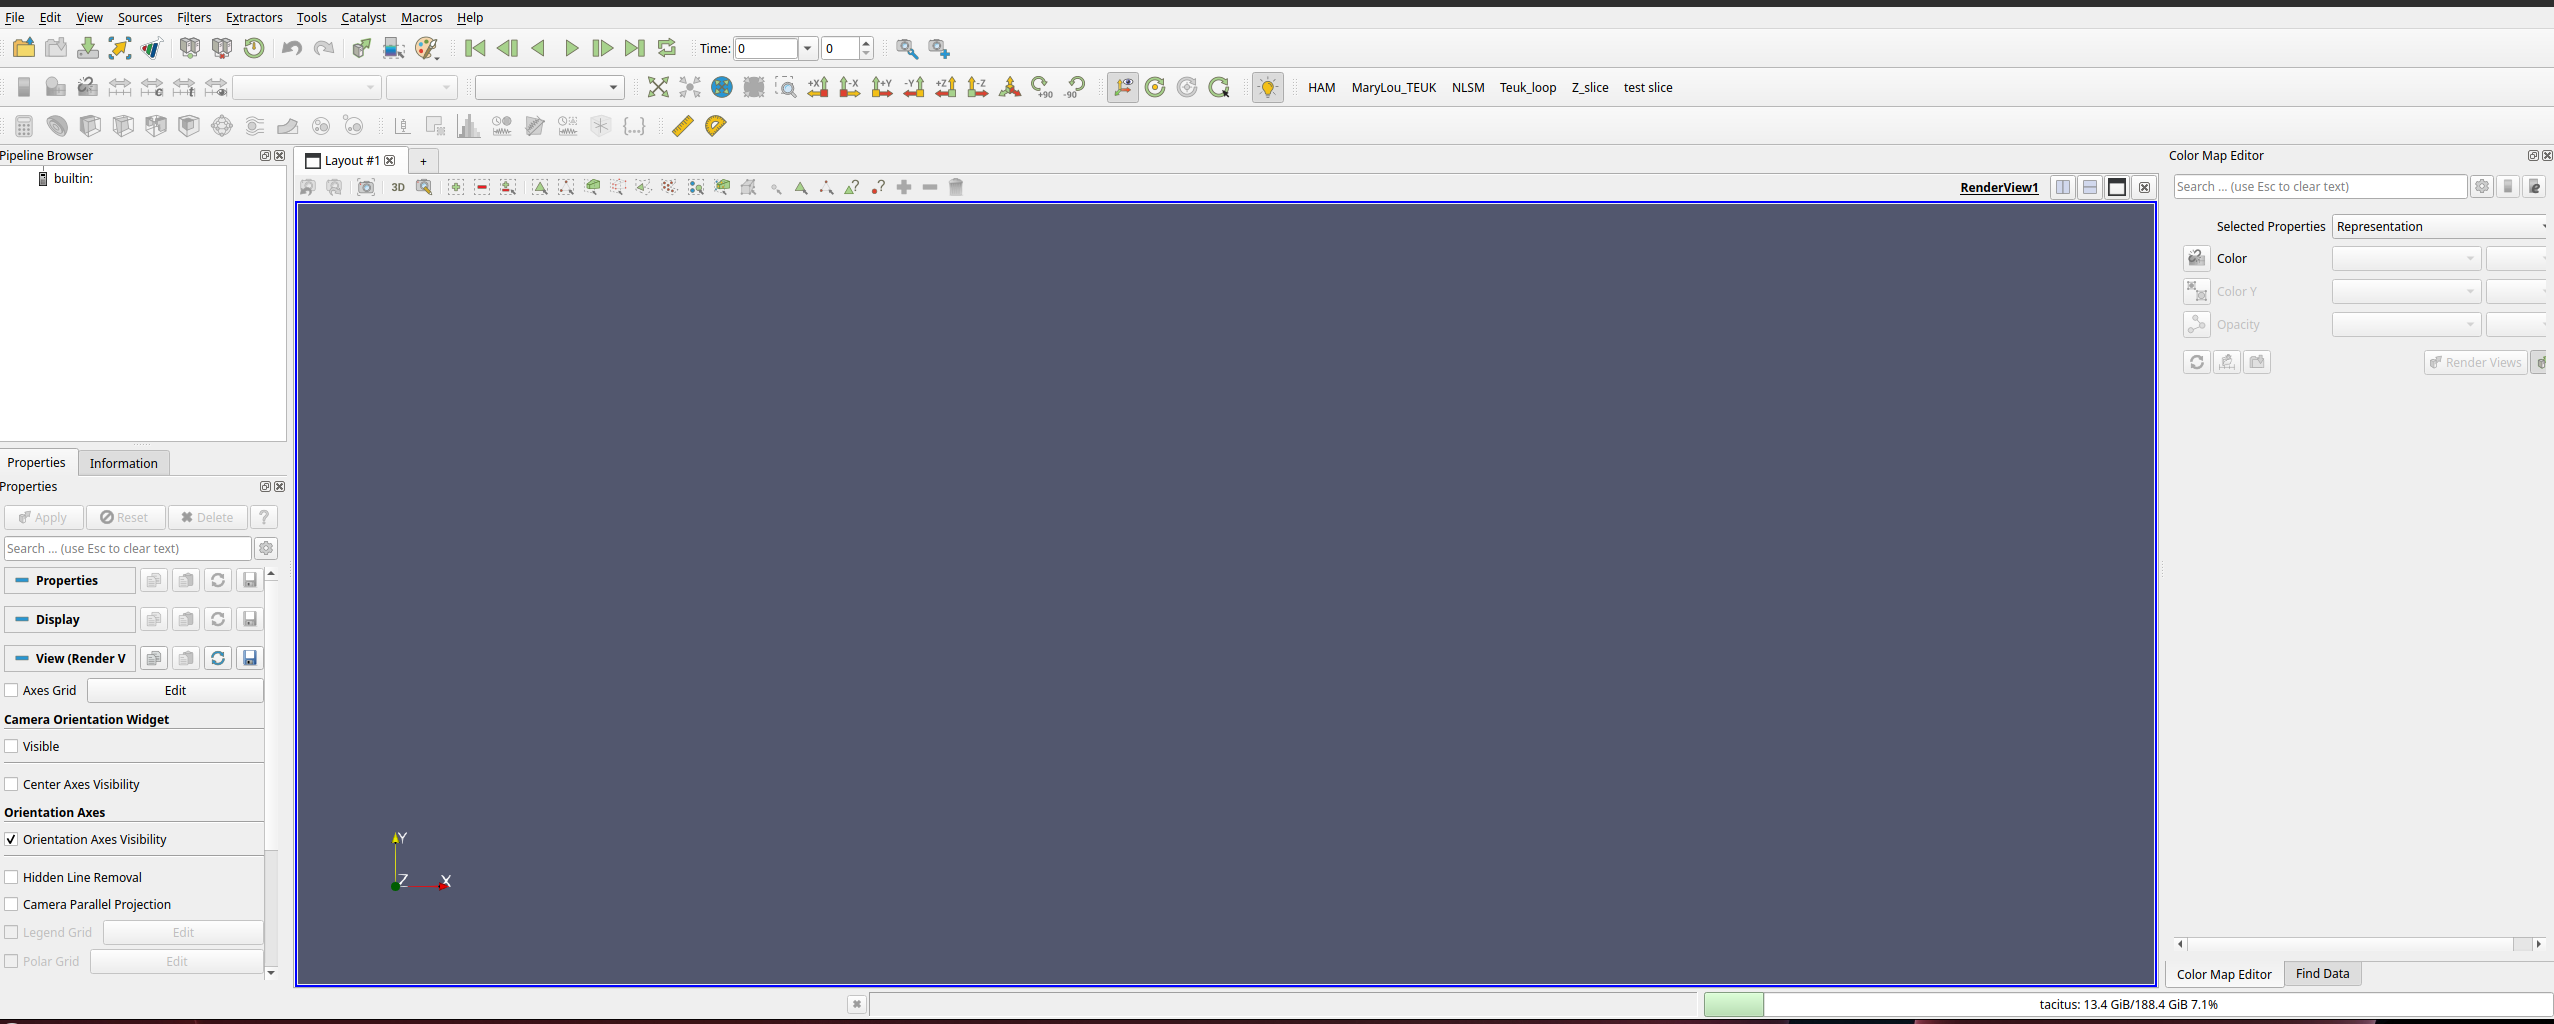
\includegraphics[width=\textwidth]{Paraview/Paraview_1.png}};

% Coordinates are scaled so that (0,0) is the bottom-left
% of the image and (1,1) is the top-right.
\begin{scope}[
    x={(img.south east)},
    y={(img.north west)}
]

    % Red box around the Open File icon
    \draw[red, very thick]
        (0.003,0.930) rectangle (0.018,0.968);

    % Arrow and label
    \draw[red, very thick, ->]
        (0.120,0.900) -- (0.018,0.955);

    \node[
        red,
        fill=white,
        draw=red,
        thick,
        rounded corners,
        font=\small
    ] at (0.180,0.890)
        {Open File};

\end{scope}

\end{tikzpicture}

\caption[Opening simulation data in ParaView]{
The ParaView interface with the \textbf{Open File} icon highlighted.
}
\label{fig:paraview_open}

\end{figure}

After clicking the \textbf{Open File} button, navigate to the directory where
the simulation output is saved. Dendro commonly writes visualization data in
\texttt{.vtu} format, which stands for \emph{VTK Unstructured Grid}. For
parallel runs, the output is often accompanied by a \texttt{.pvtu} file. The
\texttt{.pvtu} file acts as a wrapper that tells ParaView how the individual
\texttt{.vtu} pieces fit together.

In most cases, one should open the \texttt{.pvtu} file rather than opening the
individual \texttt{.vtu} files by hand. This allows ParaView to load the full
parallel dataset as a single object.

\section{Creating a Slice}
\label{sec:paraview-creating-slice}

Once the data has been loaded, a common operation is to create a two-dimensional
slice through the three-dimensional dataset. In this example, the
\textbf{Slice} tool is used to create a slice through the data, as shown in
Fig.~\ref{fig:paraview-slice-button}.

\begin{figure}[h!]
\centering

\begin{tikzpicture}
% Main screenshot
\node[anchor=south west, inner sep=0] (img) at (0,0)
{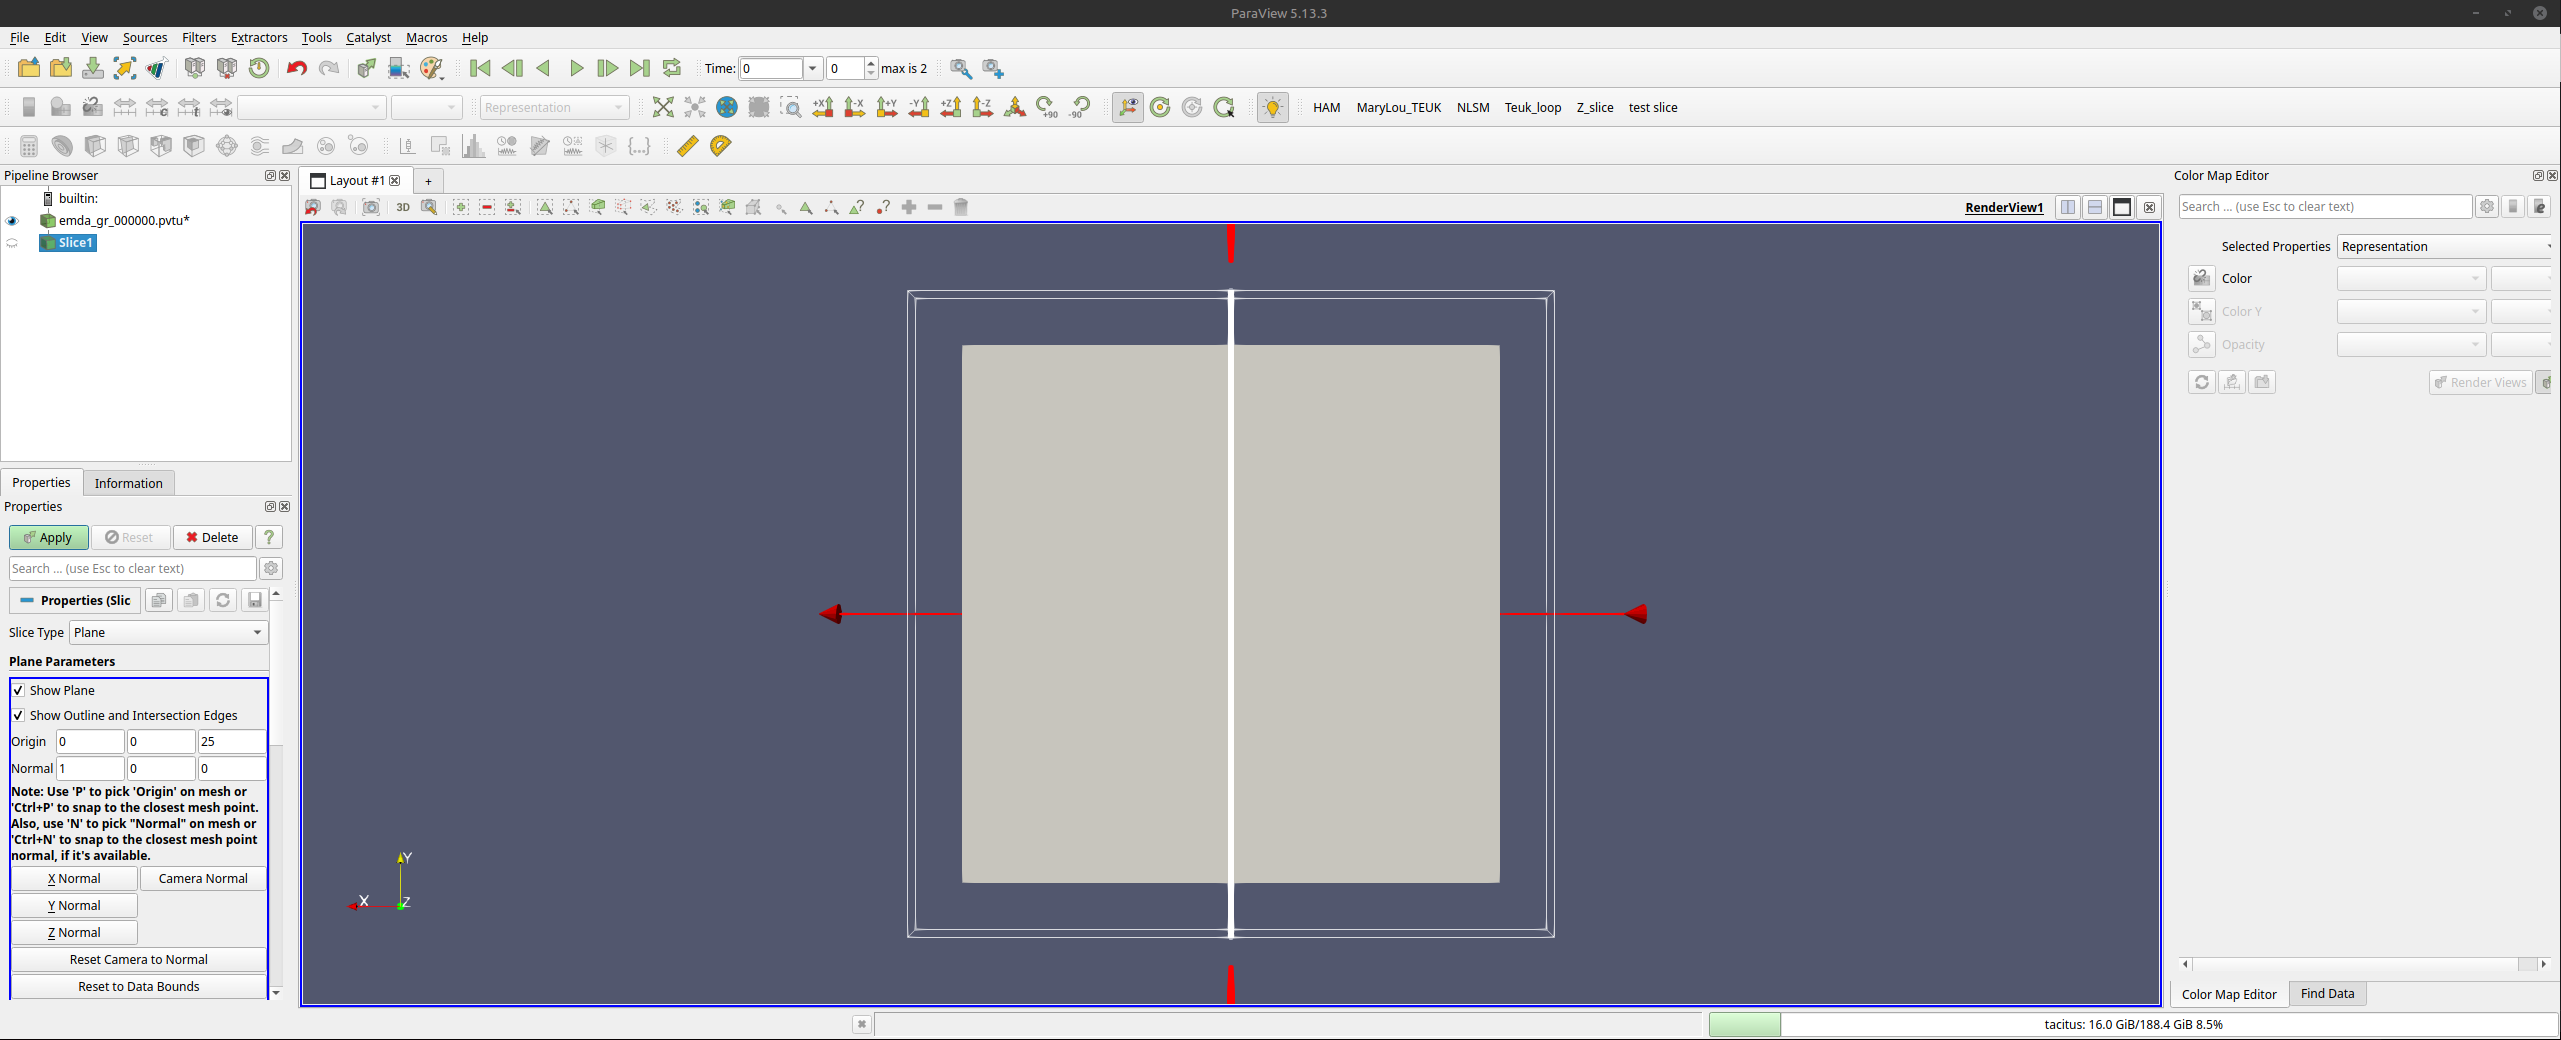
\includegraphics[width=\textwidth]{Paraview/Paraview_3.png}};

% Normalized image coordinates:
% (0,0) = bottom-left, (1,1) = top-right.
\begin{scope}[
x={(img.south east)},
y={(img.north west)}
]

```
% Box around the Slice toolbar button
\draw[red, very thick]
    (0.04415,0.847) rectangle (0.05842,0.877);

% Arrow and label for Slice
\draw[red, very thick, ->]
    (0.3215,0.70) -- (0.06,0.860);

\node[
    red,
    fill=white,
    draw=red,
    thick,
    rounded corners,
    font=\small
] at (0.33,0.69)
    {Slice};

% Box around the Calculator toolbar button
\draw[blue, very thick]
    (0.006,0.84) rectangle (0.018,0.88);

% Arrow and label for Calculator
\draw[blue, very thick, ->]
    (0.25,0.36) -- (0.018,0.840);

\node[
    blue,
    fill=white,
    draw=blue,
    thick,
    rounded corners,
    font=\small
] at (0.25,0.36)
    {Calculator};
```

\end{scope}

\end{tikzpicture}

\caption[ParaView Slice and Calculator tools]{
The ParaView interface with the \textbf{Slice} and \textbf{Calculator} tools
highlighted.
}
\label{fig:paraview_slice_button}

\end{figure}


After selecting the \textbf{Slice} tool, ParaView displays the slice settings
in the Properties panel. These settings determine the location and orientation
of the slicing plane.

\section{Adjusting the Slice and Viewing Data}
\label{sec:paraview-adjusting-slice}

ParaView allows the user to choose how the data should be sliced. Often, we want
to create $z$-slices, since this is the default orientation used for many
Dendro visualizations. To do this, set the slice normal to $(0,0,1)$. We also
set the origin to $(0,0,10^{-5})$. The small nonzero $z$-value is used because
setting the slice exactly at $z=0$ can sometimes cause ParaView to miss cells
lying on the symmetry plane.

The \textbf{Show Plane} option should be turned off so that only the data slice
is displayed. After changing these settings, click \textbf{Apply}.

Once the slice is displayed, the visualized field can be changed using the
field-selection menu. The available time steps can be explored using the time
controls, and the representation menu can be used to switch between viewing
modes such as \textbf{Surface} and \textbf{Wireframe}. These controls are
highlighted in Fig.~\ref{fig:paraview-view-controls}.

\begin{figure}[h!]
\centering

\begin{tikzpicture}
% Main screenshot
\node[anchor=south west, inner sep=0] (img) at (0,0)
{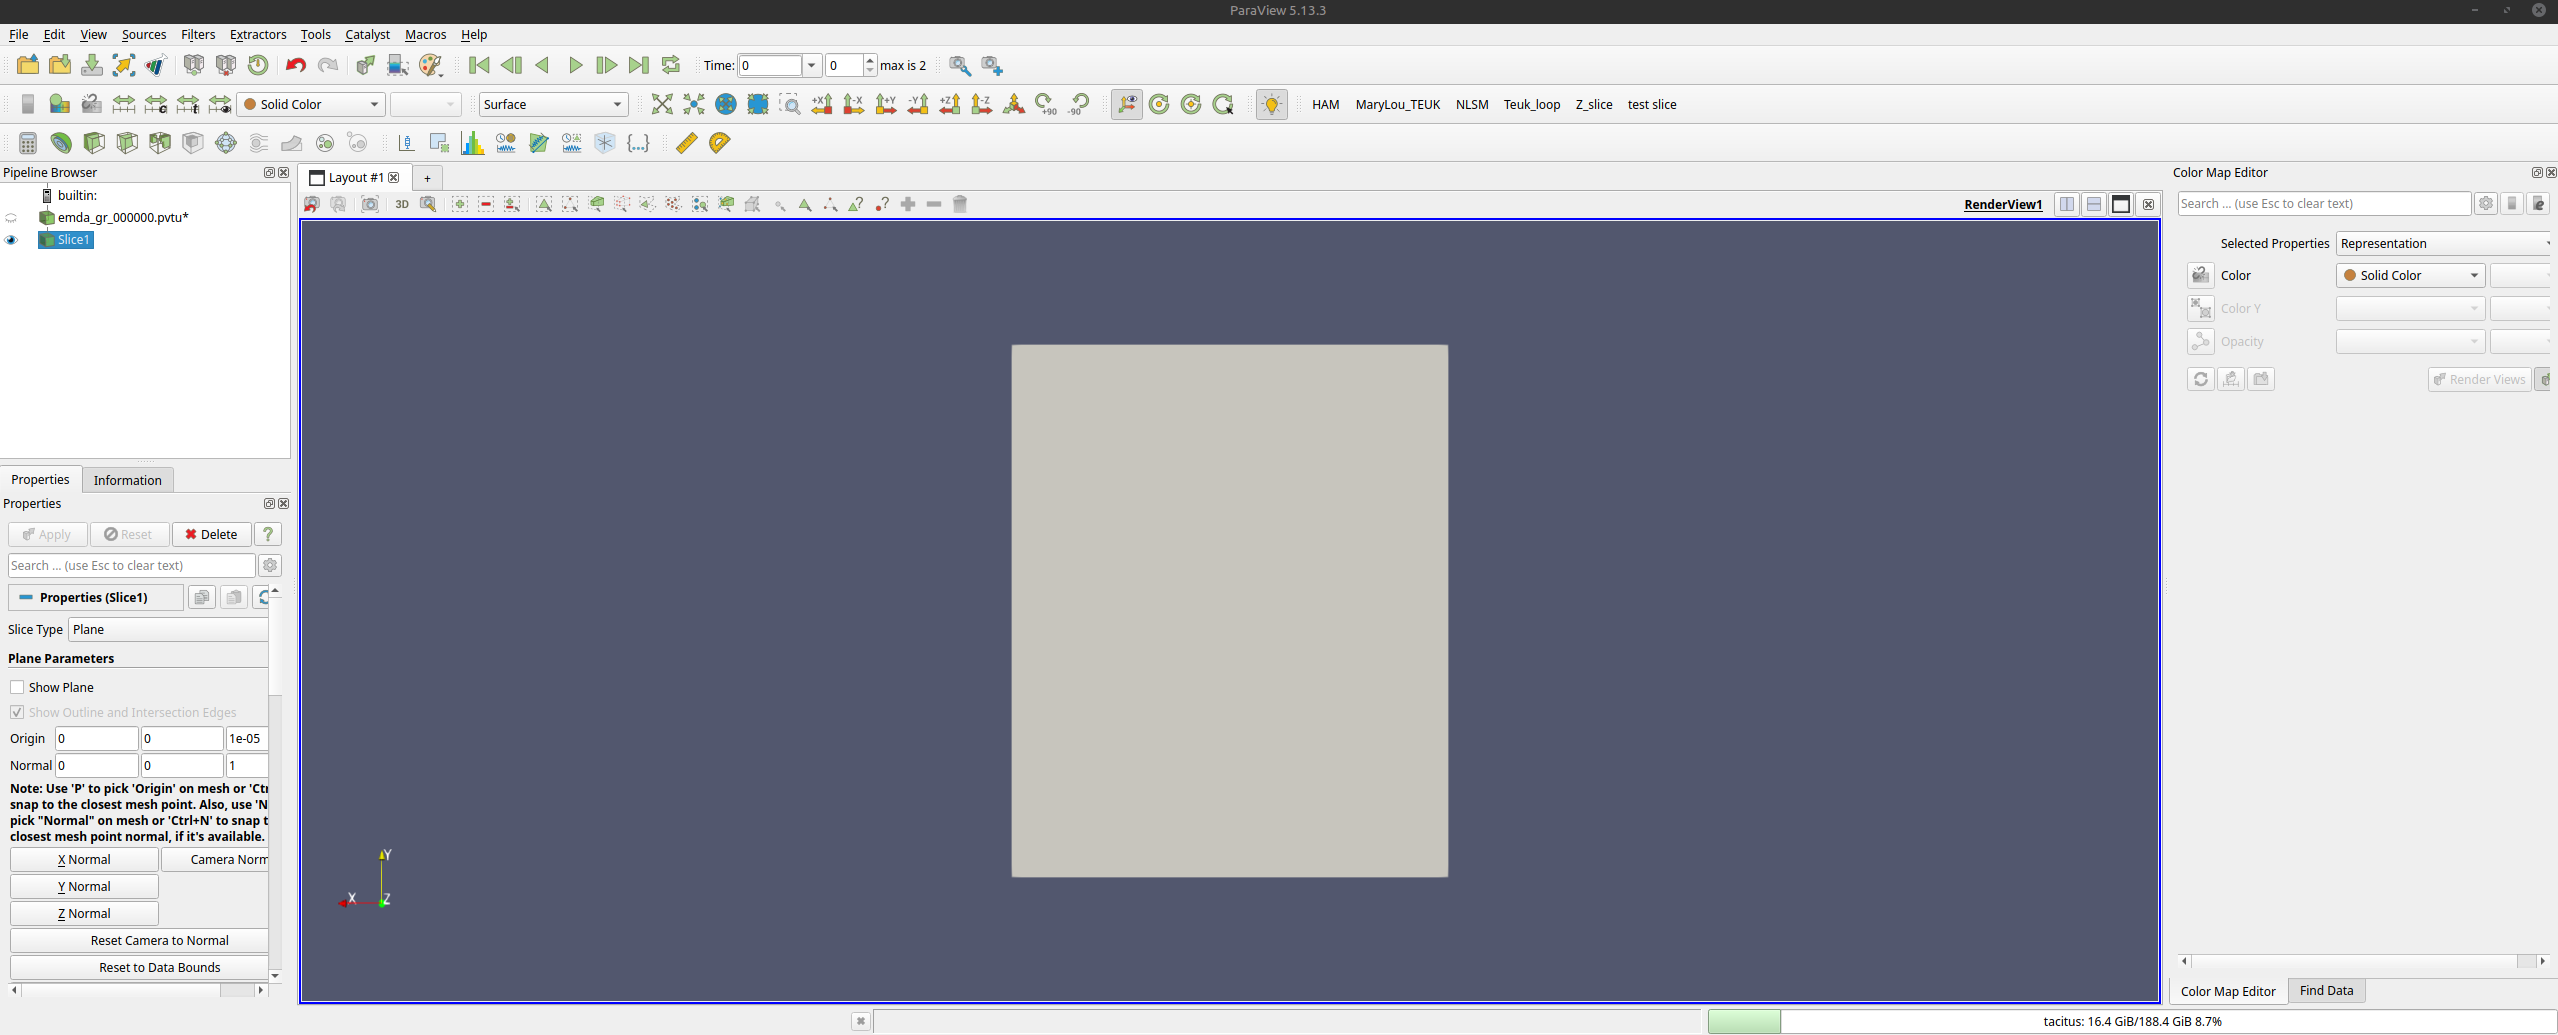
\includegraphics[width=\textwidth]{Paraview/Paraview_5.png}};

% Normalized image coordinates:
% (0,0) = bottom-left, (1,1) = top-right.
\begin{scope}[
x={(img.south east)},
y={(img.north west)}
]

```
% Time controls: play/pause and step forward/backward buttons
\draw[red, very thick]
    (0.18,0.921) rectangle (0.26,0.955);

\draw[red, very thick, ->]
    (0.330,0.975) -- (0.262,0.93);

\node[
    red,
    fill=white,
    draw=red,
    thick,
    rounded corners,
    font=\small
] at (0.385,0.975)
    {Time controls};

% Solid Color dropdown
\draw[blue, very thick]
    (0.087,0.885) rectangle (0.150,0.916);

\draw[blue, very thick, ->]
    (0.055,0.845) -- (0.118,0.883);

\node[
    blue,
    fill=white,
    draw=blue,
    thick,
    rounded corners,
    font=\small
] at (0.030,0.840)
    {Fields};

% Surface/Wireframe dropdown
\draw[green, very thick]
    (0.187,0.880) rectangle (0.245,0.916);

\draw[green, very thick, ->]
    (0.315,0.83) -- (0.246,0.890);

\node[
    green,
    fill=white,
    draw=green,
    thick,
    rounded corners,
    font=\small
] at (0.375,0.840)
    {Surface / Wireframe};
```

\end{scope}

\end{tikzpicture}

\caption[ParaView visualization and time controls]{
ParaView controls for stepping through time, selecting the displayed field or
color option, and switching between representations such as \textbf{Surface}
and \textbf{Wireframe}.
}
\label{fig:paraview_view_controls}

\end{figure}

\section{Using the Calculator}
\label{sec:paraview-calculator}

The \textbf{Calculator} filter can be used to construct derived quantities from
the fields stored in the simulation output. After selecting the loaded dataset
or slice, click the \textbf{Calculator} button. In the Calculator panel, choose
the appropriate scalar or vector fields from the available data arrays.
Mathematical operations can then be applied to these fields to define a new
quantity for visualization or export.

For example, the Calculator can be used to rescale a field, combine multiple
fields, or construct diagnostic quantities that are not stored directly in the
output files. After entering the desired expression, click \textbf{Apply} to
create the new field.

\section{Warping by Scalar}
\label{sec:paraview-warp-by-scalar}

The \textbf{Warp By Scalar} filter can be used to displace a surface according
to the value of a scalar field. This is useful for visualizing the relative
amplitude of a field on a slice.

To use the filter, click \textbf{Filters} and search for \textbf{Warp By
Scalar}. After selecting the filter, its settings appear in the Properties
panel, in the same general location as the slice settings.

\begin{figure}[h!]
\centering

\begin{tikzpicture}
\node[anchor=south west, inner sep=0] (img) at (0,0)
{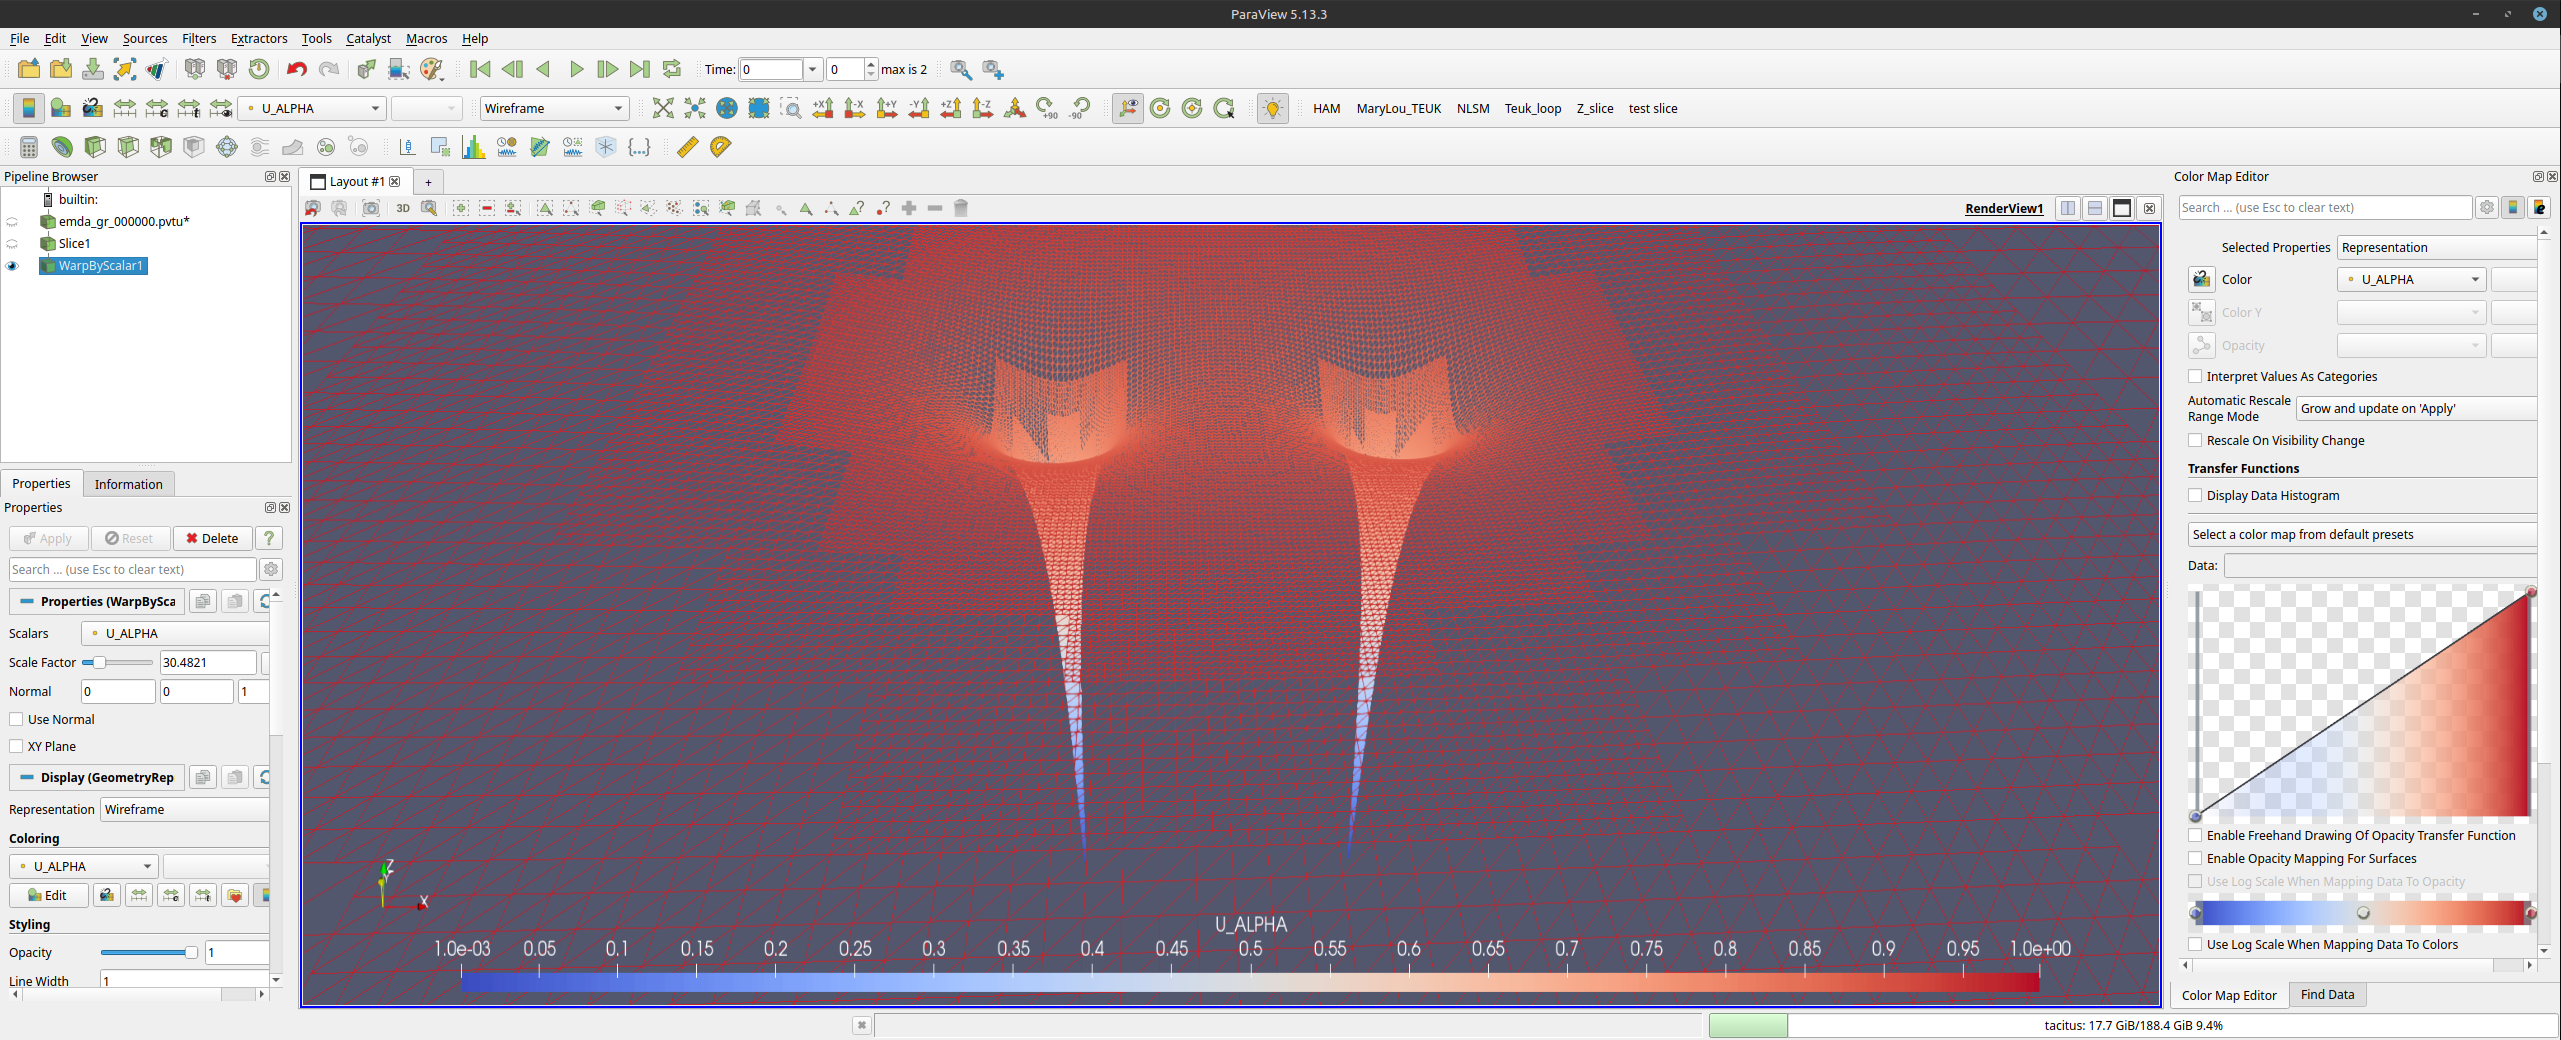
\includegraphics[width=\textwidth]{Paraview/Paraview_6.png}};

\begin{scope}[
x={(img.south east)},
y={(img.north west)}
]

```
% Scalars dropdown
\draw[red, very thick]
    (0.031,0.380) rectangle (0.084,0.410);

\draw[red, very thick, ->]
    (0.200,0.440) -- (0.085,0.410);

\node[
    red,
    fill=white,
    draw=red,
    thick,
    rounded corners,
    font=\small
] at (0.205,0.450)
    {Scalars};

% Scale Factor control
\draw[blue, very thick]
    (0.000,0.350) rectangle (0.100,0.381);

\draw[blue, very thick, ->]
    (0.165,0.360) -- (0.100,0.350);

\node[
    blue,
    fill=white,
    draw=blue,
    thick,
    rounded corners,
    font=\small
] at (0.235,0.360)
    {Scale Factor};
```

\end{scope}

\end{tikzpicture}

\caption[ParaView Warp By Scalar settings]{
The \textbf{Warp By Scalar} settings in the Properties panel. The
\textbf{Scalars} menu selects the field used for the warping, and the
\textbf{Scale Factor} controls the strength of the warp.
}
\label{fig:paraview_warp_by_scalar}

\end{figure}


In the \textbf{Scalars} menu, select the field that should determine the warp.
The \textbf{Scale Factor} controls the strength of the displacement. Large scale
factors can make small-amplitude fields easier to see, but they can also distort
the visualization if chosen too large.

\section{Using the Color Map Editor}
\label{sec:paraview-color-map-editor}

The \textbf{Color Map Editor} controls how ParaView maps data values to colors.
It can be used to change the color scale, adjust the visible data range, modify
opacity, and choose a different color preset.

\begin{figure}[p]
\centering

\includegraphics[
width=\textwidth,
height=0.75\textheight,
keepaspectratio
]{Paraview/Paraview_7.png}

\caption[ParaView Color Map Editor]{
The \textbf{Color Map Editor} panel in ParaView. This panel controls the color
scale, opacity, and transfer function used to visualize the selected field.
}
\label{fig:paraview_color_map_editor}

\end{figure}


By default, the color mapping may not automatically update when stepping
through time. The easiest way to ensure that the colors match the data range at
each time step is to rescale the color range when the time step changes. This
prevents the visualization from using an outdated color range from a previous
time step.

\section{Macros, Animations, CSV Output, and Finding Data}
\label{sec:paraview-macros-output-find-data}

Often, we want to repeat the same visualization or post-processing steps for
many datasets. ParaView can automate these repetitive tasks using macros. To
create a macro, click \textbf{Tools} and select \textbf{Start Trace}. Then
perform the sequence of actions that should be automated. When finished, click
\textbf{Stop Trace}. ParaView will then allow the recorded trace to be saved as
a Python script or macro, which can later be reused.

ParaView can also save the currently loaded data as a CSV file. To do this,
click \textbf{File} and select \textbf{Save Data}. This saves the data from the
currently active object, such as the current slice. The resulting CSV file can
then be loaded into Python, MATLAB, Mathematica, or another analysis tool.

Animations can be saved by clicking \textbf{File} and selecting
\textbf{Save Animation}. This is useful for producing movies that show the time
evolution of a field.

Finally, ParaView can be used to find data that satisfies certain conditions.
To do this, click \textbf{View} and select \textbf{Find Data}. In the
\textbf{Find Data} panel, choose the dataset to search. The element type can
usually be left as \textbf{Point}. Then choose the field to search, set the
desired condition and value, and click \textbf{Find Data}. The matching region
will be highlighted in the render view.


\chapter{Waveform Catalog}
\section{Gravitational Waveform Catalog}
\label{app:gw_waveform_catalog}

The following figures show the extracted \(r\Psi_4^{(2,2)}\) waveforms at
\(r\simeq 100M\). For each mass ratio and spin, the neutral case is shown
above the charged configurations. The charged cases are ordered by charge
magnitude and charge configuration.

% Compact waveform panel macro.
% This version is compatible with \usepackage[caption=false]{subfig}.
\newcommand{\gwpanel}[1]{%
    \subfloat[]{%
        \includegraphics[width=0.315\textwidth]{#1}%
    }%
}

\newcommand{\gwneutralpanel}[1]{%
    \subfloat[]{%
        \includegraphics[width=0.315\textwidth]{#1}%
    }%
}

% ============================================================
% q = 1, chi = 0
% ============================================================
\begin{figure}[p]
\centering

\gwneutralpanel{Waveform/GW/Q1_SPIN_0_Q0_emda_prof_GW_l2_m2_r5.pdf}

\vspace{0.6em}

\gwpanel{Waveform/GW/Q1_SPIN_0_Q0p05_p0_emda_prof_GW_l2_m2_r5.pdf}
\hfill
\gwpanel{Waveform/GW/Q1_SPIN_0_Q0p05_pn_emda_prof_GW_l2_m2_r5.pdf}
\hfill
\gwpanel{Waveform/GW/Q1_SPIN_0_Q0p05_pp_emda_prof_GW_l2_m2_r5.pdf}

\vspace{0.6em}

\gwpanel{Waveform/GW/Q1_SPIN_0_Q0p1_p0_emda_prof_GW_l2_m2_r5.pdf}
\hfill
\gwpanel{Waveform/GW/Q1_SPIN_0_Q0p1_pn_emda_prof_GW_l2_m2_r5.pdf}
\hfill
\gwpanel{Waveform/GW/Q1_SPIN_0_Q0p1_pp_emda_prof_GW_l2_m2_r5.pdf}

\vspace{0.6em}

\gwpanel{Waveform/GW/Q1_SPIN_0_Q0p15_p0_emda_prof_GW_l2_m2_r5.pdf}
\hfill
\gwpanel{Waveform/GW/Q1_SPIN_0_Q0p15_pn_emda_prof_GW_l2_m2_r5.pdf}
\hfill
\gwpanel{Waveform/GW/Q1_SPIN_0_Q0p15_pp_emda_prof_GW_l2_m2_r5.pdf}

\caption{Extracted \(r\Psi_4^{(2,2)}\) waveforms for \(q=1\) and \(\chi=0\). The neutral case is shown at the top, followed by charged configurations ordered by increasing charge magnitude and charge configuration.}
\label{fig:gw_catalog_q1_chi0}
\end{figure}

% ============================================================
% q = 1, chi = 0.4
% ============================================================
\begin{figure}[p]
\centering

\gwneutralpanel{Waveform/GW/Q1_SPIN_04_Q0_emda_prof_GW_l2_m2_r5.pdf}

\vspace{0.6em}

\gwpanel{Waveform/GW/Q1_SPIN_04_Q0p05_p0_emda_prof_GW_l2_m2_r5.pdf}
\hfill
\gwpanel{Waveform/GW/Q1_SPIN_04_Q0p05_pn_emda_prof_GW_l2_m2_r5.pdf}
\hfill
\gwpanel{Waveform/GW/Q1_SPIN_04_Q0p05_pp_emda_prof_GW_l2_m2_r5.pdf}

\vspace{0.6em}

\gwpanel{Waveform/GW/Q1_SPIN_04_Q0p1_p0_emda_prof_GW_l2_m2_r5.pdf}
\hfill
\gwpanel{Waveform/GW/Q1_SPIN_04_Q0p1_pn_emda_prof_GW_l2_m2_r5.pdf}
\hfill
\gwpanel{Waveform/GW/Q1_SPIN_04_Q0p1_pp_emda_prof_GW_l2_m2_r5.pdf}

\vspace{0.6em}

\gwpanel{Waveform/GW/Q1_SPIN_04_Q0p15_p0_emda_prof_GW_l2_m2_r5.pdf}
\hfill
\gwpanel{Waveform/GW/Q1_SPIN_04_Q0p15_pn_emda_prof_GW_l2_m2_r5.pdf}
\hfill
\gwpanel{Waveform/GW/Q1_SPIN_04_Q0p15_pp_emda_prof_GW_l2_m2_r5.pdf}

\caption{Extracted \(r\Psi_4^{(2,2)}\) waveforms for \(q=1\) and \(\chi=0.4\). The neutral case is shown at the top, followed by charged configurations ordered by increasing charge magnitude and charge configuration.}
\label{fig:gw_catalog_q1_chi04}
\end{figure}

% ============================================================
% q = 1, chi = 0.8
% ============================================================
\begin{figure}[p]
\centering

\gwneutralpanel{Waveform/GW/Q1_SPIN_08_Q0_emda_prof_GW_l2_m2_r5.pdf}

\vspace{0.6em}

\gwpanel{Waveform/GW/Q1_SPIN_08_Q0p05_p0_emda_prof_GW_l2_m2_r5.pdf}
\hfill
\gwpanel{Waveform/GW/Q1_SPIN_08_Q0p05_pn_emda_prof_GW_l2_m2_r5.pdf}
\hfill
\gwpanel{Waveform/GW/Q1_SPIN_08_Q0p05_pp_emda_prof_GW_l2_m2_r5.pdf}

\vspace{0.6em}

\gwpanel{Waveform/GW/Q1_SPIN_08_Q0p1_p0_emda_prof_GW_l2_m2_r5.pdf}
\hfill
\gwpanel{Waveform/GW/Q1_SPIN_08_Q0p1_pn_emda_prof_GW_l2_m2_r5.pdf}
\hfill
\gwpanel{Waveform/GW/Q1_SPIN_08_Q0p1_pp_emda_prof_GW_l2_m2_r5.pdf}

\vspace{0.6em}

\gwpanel{Waveform/GW/Q1_SPIN_08_Q0p15_p0_emda_prof_GW_l2_m2_r5.pdf}
\hfill
\gwpanel{Waveform/GW/Q1_SPIN_08_Q0p15_pn_emda_prof_GW_l2_m2_r5.pdf}
\hfill
\gwpanel{Waveform/GW/Q1_SPIN_08_Q0p15_pp_emda_prof_GW_l2_m2_r5.pdf}

\caption{Extracted \(r\Psi_4^{(2,2)}\) waveforms for \(q=1\) and \(\chi=0.8\). The neutral case is shown at the top, followed by charged configurations ordered by increasing charge magnitude and charge configuration.}
\label{fig:gw_catalog_q1_chi08}
\end{figure}

% ============================================================
% q = 2, chi = 0
% ============================================================
\begin{figure}[p]
\centering

\gwneutralpanel{Waveform/GW/Q2_SPIN_0_Q0_emda_prof_GW_l2_m2_r5.pdf}

\vspace{0.6em}

\gwpanel{Waveform/GW/Q2_SPIN_0_Q0p05_p0_emda_prof_GW_l2_m2_r5.pdf}
\hfill
\gwpanel{Waveform/GW/Q2_SPIN_0_Q0p05_pn_emda_prof_GW_l2_m2_r5.pdf}
\hfill
\gwpanel{Waveform/GW/Q2_SPIN_0_Q0p05_pp_emda_prof_GW_l2_m2_r5.pdf}

\vspace{0.6em}

\gwpanel{Waveform/GW/Q2_SPIN_0_Q0p15_p0_emda_prof_GW_l2_m2_r5.pdf}
\hfill
\gwpanel{Waveform/GW/Q2_SPIN_0_Q0p15_pn_emda_prof_GW_l2_m2_r5.pdf}
\hfill
\gwpanel{Waveform/GW/Q2_SPIN_0_Q0p15_pp_emda_prof_GW_l2_m2_r5.pdf}

\caption{Extracted \(r\Psi_4^{(2,2)}\) waveforms for \(q=2\) and \(\chi=0\). The neutral case is shown at the top, followed by charged configurations ordered by increasing charge magnitude and charge configuration.}
\label{fig:gw_catalog_q2_chi0}
\end{figure}

% ============================================================
% q = 2, chi = 0.4
% ============================================================
\begin{figure}[p]
\centering

\gwneutralpanel{Waveform/GW/Q2_SPIN_04_Q0_emda_prof_GW_l2_m2_r5.pdf}

\vspace{0.6em}

\gwpanel{Waveform/GW/Q2_SPIN_04_Q0p05_p0_emda_prof_GW_l2_m2_r5.pdf}
\hfill
\gwpanel{Waveform/GW/Q2_SPIN_04_Q0p05_pn_emda_prof_GW_l2_m2_r5.pdf}
\hfill
\gwpanel{Waveform/GW/Q2_SPIN_04_Q0p05_pp_emda_prof_GW_l2_m2_r5.pdf}

\vspace{0.6em}

\gwpanel{Waveform/GW/Q2_SPIN_04_Q0p15_p0_emda_prof_GW_l2_m2_r5.pdf}
\hfill
\gwpanel{Waveform/GW/Q2_SPIN_04_Q0p15_pn_emda_prof_GW_l2_m2_r5.pdf}
\hfill
\gwpanel{Waveform/GW/Q2_SPIN_04_Q0p15_pp_emda_prof_GW_l2_m2_r5.pdf}

\caption{Extracted \(r\Psi_4^{(2,2)}\) waveforms for \(q=2\) and \(\chi=0.4\). The neutral case is shown at the top, followed by charged configurations ordered by increasing charge magnitude and charge configuration.}
\label{fig:gw_catalog_q2_chi04}
\end{figure}

% ============================================================
% q = 4, chi = 0.4
% ============================================================
\begin{figure}[p]
\centering

\gwneutralpanel{Waveform/GW/Q4_SPIN_04_Q0_emda_prof_GW_l2_m2_r5.pdf}

\vspace{0.6em}

\gwpanel{Waveform/GW/Q4_SPIN_04_Q0p05_p0_emda_prof_GW_l2_m2_r5.pdf}
\hfill
\gwpanel{Waveform/GW/Q4_SPIN_04_Q0p05_pn_emda_prof_GW_l2_m2_r5.pdf}
\hfill
\gwpanel{Waveform/GW/Q4_SPIN_04_Q0p05_pp_emda_prof_GW_l2_m2_r5.pdf}

\caption{Extracted \(r\Psi_4^{(2,2)}\) waveforms for \(q=4\) and \(\chi=0.4\). The neutral case is shown at the top, followed by the charged configurations.}
\label{fig:gw_catalog_q4_chi04}
\end{figure}

% ============================================================
% q = 8, chi = 0.2
% ============================================================
\begin{figure}[p]
\centering

\subfloat[Neutral configuration.]{%
    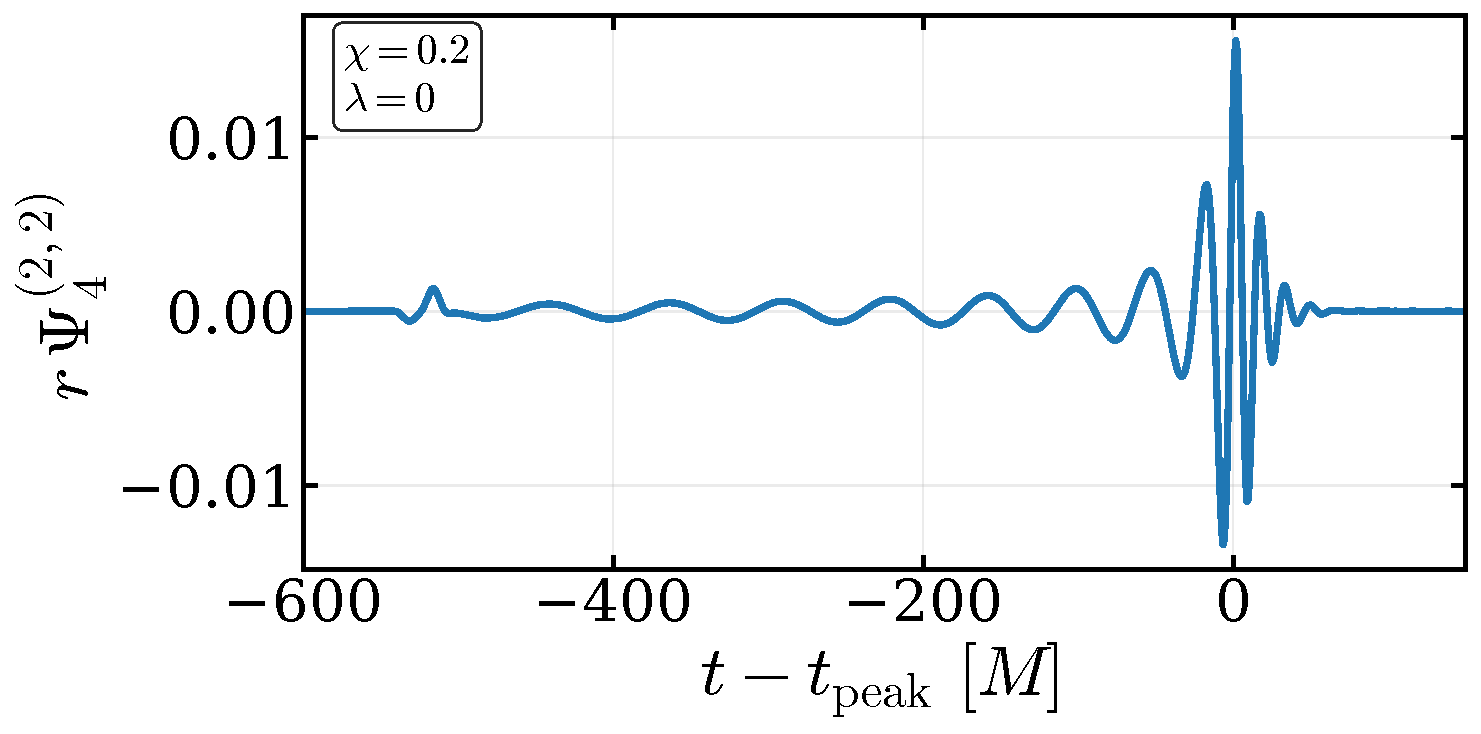
\includegraphics[width=0.47\textwidth]{Waveform/GW/Q8_SPIN_02_Q0_emda_prof_GW_l2_m2_r5.pdf}%
}
\hfill
\subfloat[Charged \(++\) configuration.]{%
    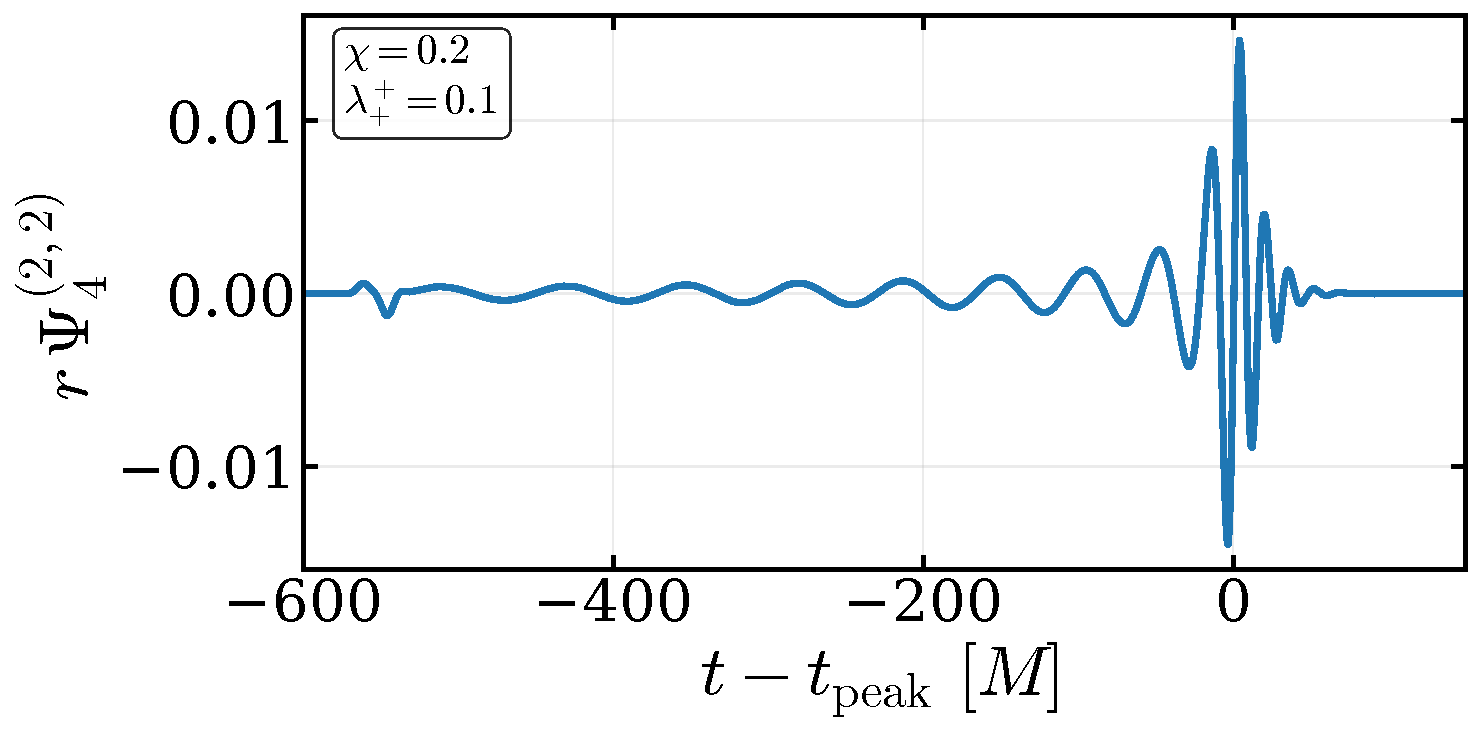
\includegraphics[width=0.47\textwidth]{Waveform/GW/Q8_SPIN_02_Q0p1_pp_emda_prof_GW_l2_m2_r5.pdf}%
}

\caption{Extracted \(r\Psi_4^{(2,2)}\) waveforms for \(q=8\) and \(\chi=0.2\).}
\label{fig:gw_catalog_q8_chi02}
\end{figure}

% ============================================================
% Scalar waveform catalog macros
% Compatible with \usepackage[caption=false]{subfig}
% ============================================================

\newcommand{\fieldpanel}[2]{%
    \subfloat[#1]{%
        \includegraphics[width=0.315\textwidth]{#2}%
    }%
}

% ============================================================
% PHI1 waveform catalog
% ============================================================
\section{\texorpdfstring{\(\Phi_1\)}{Phi1} Waveform Catalog}
\label{app:phi1_waveform_catalog}

The following figures show the extracted \(\Phi_1\) waveforms at
\(r\simeq 100M\). Since there is no radiation in the neutral case,
only charged configurations are shown. The charged cases are ordered
by charge magnitude and charge configuration. For the \(+-\) cases,
we show the \((\ell,m)=(1,1)\) mode, while for the \(+0\) and \(++\)
cases we show the \((\ell,m)=(2,2)\) mode.

% ============================================================
% PHI1: q = 1, chi = 0
% ============================================================
\begin{figure}[p]
\centering

\fieldpanel{\(Q0p05,+0\)}
{Waveform/PHI1/Q1_SPIN_0_Q0p05_p0_emda_prof_PHI1_l2_m2_r5.pdf}
\hfill
\fieldpanel{\(Q0p05,+-\)}
{Waveform/PHI1/Q1_SPIN_0_Q0p05_pn_emda_prof_PHI1_l1_m1_r5.pdf}
\hfill
\fieldpanel{\(Q0p05,++\)}
{Waveform/PHI1/Q1_SPIN_0_Q0p05_pp_emda_prof_PHI1_l2_m2_r5.pdf}

\vspace{0.6em}

\fieldpanel{\(Q0p1,+0\)}
{Waveform/PHI1/Q1_SPIN_0_Q0p1_p0_emda_prof_PHI1_l2_m2_r5.pdf}
\hfill
\fieldpanel{\(Q0p1,+-\)}
{Waveform/PHI1/Q1_SPIN_0_Q0p1_pn_emda_prof_PHI1_l1_m1_r5.pdf}
\hfill
\fieldpanel{\(Q0p1,++\)}
{Waveform/PHI1/Q1_SPIN_0_Q0p1_pp_emda_prof_PHI1_l2_m2_r5.pdf}

\vspace{0.6em}

\fieldpanel{\(Q0p15,+0\)}
{Waveform/PHI1/Q1_SPIN_0_Q0p15_p0_emda_prof_PHI1_l2_m2_r5.pdf}
\hfill
\fieldpanel{\(Q0p15,+-\)}
{Waveform/PHI1/Q1_SPIN_0_Q0p15_pn_emda_prof_PHI1_l1_m1_r5.pdf}
\hfill
\fieldpanel{\(Q0p15,++\)}
{Waveform/PHI1/Q1_SPIN_0_Q0p15_pp_emda_prof_PHI1_l2_m2_r5.pdf}

\caption{Extracted \(\Phi_1\) waveforms for \(q=1\) and \(\chi=0\).}
\label{fig:phi1_catalog_q1_chi0}
\end{figure}

% ============================================================
% PHI1: q = 1, chi = 0.4
% ============================================================
\begin{figure}[p]
\centering

\fieldpanel{\(Q0p05,+0\)}
{Waveform/PHI1/Q1_SPIN_04_Q0p05_p0_emda_prof_PHI1_l2_m2_r5.pdf}
\hfill
\fieldpanel{\(Q0p05,+-\)}
{Waveform/PHI1/Q1_SPIN_04_Q0p05_pn_emda_prof_PHI1_l1_m1_r5.pdf}
\hfill
\fieldpanel{\(Q0p05,++\)}
{Waveform/PHI1/Q1_SPIN_04_Q0p05_pp_emda_prof_PHI1_l2_m2_r5.pdf}

\vspace{0.6em}

\fieldpanel{\(Q0p1,+0\)}
{Waveform/PHI1/Q1_SPIN_04_Q0p1_p0_emda_prof_PHI1_l2_m2_r5.pdf}
\hfill
\fieldpanel{\(Q0p1,+-\)}
{Waveform/PHI1/Q1_SPIN_04_Q0p1_pn_emda_prof_PHI1_l1_m1_r5.pdf}
\hfill
\fieldpanel{\(Q0p1,++\)}
{Waveform/PHI1/Q1_SPIN_04_Q0p1_pp_emda_prof_PHI1_l2_m2_r5.pdf}

\vspace{0.6em}

\fieldpanel{\(Q0p15,+0\)}
{Waveform/PHI1/Q1_SPIN_04_Q0p15_p0_emda_prof_PHI1_l2_m2_r5.pdf}
\hfill
\fieldpanel{\(Q0p15,+-\)}
{Waveform/PHI1/Q1_SPIN_04_Q0p15_pn_emda_prof_PHI1_l1_m1_r5.pdf}
\hfill
\fieldpanel{\(Q0p15,++\)}
{Waveform/PHI1/Q1_SPIN_04_Q0p15_pp_emda_prof_PHI1_l2_m2_r5.pdf}

\caption{Extracted \(\Phi_1\) waveforms for \(q=1\) and \(\chi=0.4\).}
\label{fig:phi1_catalog_q1_chi04}
\end{figure}

% ============================================================
% PHI1: q = 1, chi = 0.8
% ============================================================
\begin{figure}[p]
\centering

\fieldpanel{\(Q0p05,+0\)}
{Waveform/PHI1/Q1_SPIN_08_Q0p05_p0_emda_prof_PHI1_l2_m2_r5.pdf}
\hfill
\fieldpanel{\(Q0p05,+-\)}
{Waveform/PHI1/Q1_SPIN_08_Q0p05_pn_emda_prof_PHI1_l1_m1_r5.pdf}
\hfill
\fieldpanel{\(Q0p05,++\)}
{Waveform/PHI1/Q1_SPIN_08_Q0p05_pp_emda_prof_PHI1_l2_m2_r5.pdf}

\vspace{0.6em}

\fieldpanel{\(Q0p1,+0\)}
{Waveform/PHI1/Q1_SPIN_08_Q0p1_p0_emda_prof_PHI1_l2_m2_r5.pdf}
\hfill
\fieldpanel{\(Q0p1,+-\)}
{Waveform/PHI1/Q1_SPIN_08_Q0p1_pn_emda_prof_PHI1_l1_m1_r5.pdf}
\hfill
\fieldpanel{\(Q0p1,++\)}
{Waveform/PHI1/Q1_SPIN_08_Q0p1_pp_emda_prof_PHI1_l2_m2_r5.pdf}

\vspace{0.6em}

\fieldpanel{\(Q0p15,+0\)}
{Waveform/PHI1/Q1_SPIN_08_Q0p15_p0_emda_prof_PHI1_l2_m2_r5.pdf}
\hfill
\fieldpanel{\(Q0p15,+-\)}
{Waveform/PHI1/Q1_SPIN_08_Q0p15_pn_emda_prof_PHI1_l1_m1_r5.pdf}
\hfill
\fieldpanel{\(Q0p15,++\)}
{Waveform/PHI1/Q1_SPIN_08_Q0p15_pp_emda_prof_PHI1_l2_m2_r5.pdf}

\caption{Extracted \(\Phi_1\) waveforms for \(q=1\) and \(\chi=0.8\).}
\label{fig:phi1_catalog_q1_chi08}
\end{figure}

% ============================================================
% PHI1: q = 2, chi = 0
% ============================================================
\begin{figure}[p]
\centering

\fieldpanel{\(Q0p05,+0\)}
{Waveform/PHI1/Q2_SPIN_0_Q0p05_p0_emda_prof_PHI1_l2_m2_r5.pdf}
\hfill
\fieldpanel{\(Q0p05,+-\)}
{Waveform/PHI1/Q2_SPIN_0_Q0p05_pn_emda_prof_PHI1_l1_m1_r5.pdf}
\hfill
\fieldpanel{\(Q0p05,++\)}
{Waveform/PHI1/Q2_SPIN_0_Q0p05_pp_emda_prof_PHI1_l2_m2_r5.pdf}

\vspace{0.6em}

\fieldpanel{\(Q0p15,+0\)}
{Waveform/PHI1/Q2_SPIN_0_Q0p15_p0_emda_prof_PHI1_l2_m2_r5.pdf}
\hfill
\fieldpanel{\(Q0p15,+-\)}
{Waveform/PHI1/Q2_SPIN_0_Q0p15_pn_emda_prof_PHI1_l1_m1_r5.pdf}
\hfill
\fieldpanel{\(Q0p15,++\)}
{Waveform/PHI1/Q2_SPIN_0_Q0p15_pp_emda_prof_PHI1_l2_m2_r5.pdf}

\caption{Extracted \(\Phi_1\) waveforms for \(q=2\) and \(\chi=0\).}
\label{fig:phi1_catalog_q2_chi0}
\end{figure}

% ============================================================
% PHI1: q = 2, chi = 0.4
% ============================================================
\begin{figure}[p]
\centering

\fieldpanel{\(Q0p05,+0\)}
{Waveform/PHI1/Q2_SPIN_04_Q0p05_p0_emda_prof_PHI1_l2_m2_r5.pdf}
\hfill
\fieldpanel{\(Q0p05,+-\)}
{Waveform/PHI1/Q2_SPIN_04_Q0p05_pn_emda_prof_PHI1_l1_m1_r5.pdf}
\hfill
\fieldpanel{\(Q0p05,++\)}
{Waveform/PHI1/Q2_SPIN_04_Q0p05_pp_emda_prof_PHI1_l2_m2_r5.pdf}

\vspace{0.6em}

\fieldpanel{\(Q0p15,+0\)}
{Waveform/PHI1/Q2_SPIN_04_Q0p15_p0_emda_prof_PHI1_l2_m2_r5.pdf}
\hfill
\fieldpanel{\(Q0p15,+-\)}
{Waveform/PHI1/Q2_SPIN_04_Q0p15_pn_emda_prof_PHI1_l1_m1_r5.pdf}
\hfill
\fieldpanel{\(Q0p15,++\)}
{Waveform/PHI1/Q2_SPIN_04_Q0p15_pp_emda_prof_PHI1_l2_m2_r5.pdf}

\caption{Extracted \(\Phi_1\) waveforms for \(q=2\) and \(\chi=0.4\).}
\label{fig:phi1_catalog_q2_chi04}
\end{figure}

% ============================================================
% PHI1: q = 4, chi = 0.4
% ============================================================
\begin{figure}[p]
\centering

\fieldpanel{\(Q0p05,+0\)}
{Waveform/PHI1/Q4_SPIN_04_Q0p05_p0_emda_prof_PHI1_l2_m2_r5.pdf}
\hfill
\fieldpanel{\(Q0p05,+-\)}
{Waveform/PHI1/Q4_SPIN_04_Q0p05_pn_emda_prof_PHI1_l1_m1_r5.pdf}
\hfill
\fieldpanel{\(Q0p05,++\)}
{Waveform/PHI1/Q4_SPIN_04_Q0p05_pp_emda_prof_PHI1_l2_m2_r5.pdf}

\caption{Extracted \(\Phi_1\) waveforms for \(q=4\) and \(\chi=0.4\).}
\label{fig:phi1_catalog_q4_chi04}
\end{figure}

% ============================================================
% PHI1: q = 8, chi = 0.2
% ============================================================
\begin{figure}[p]
\centering

\fieldpanel{\(Q0p1,++\)}
{Waveform/PHI1/Q8_SPIN_02_Q0p1_pp_emda_prof_PHI1_l2_m2_r5.pdf}

\caption{Extracted \(\Phi_1\) waveforms for \(q=8\) and \(\chi=0.2\).}
\label{fig:phi1_catalog_q8_chi02}
\end{figure}


% ============================================================
% PHI2 waveform catalog
% ============================================================
\section{\texorpdfstring{\(\Phi_2\)}{Phi2} Waveform Catalog}
\label{app:phi2_waveform_catalog}

The following figures show the extracted \(\Phi_2\) waveforms at
\(r\simeq 100M\). Since there is no radiation in the neutral case,
only charged configurations are shown. The charged cases are ordered
by charge magnitude and charge configuration. For the \(+-\) cases,
we show the \((\ell,m)=(1,1)\) mode, while for the \(+0\) and \(++\)
cases we show the \((\ell,m)=(2,2)\) mode.

% ============================================================
% PHI2: q = 1, chi = 0
% ============================================================
\begin{figure}[p]
\centering

\fieldpanel{\(Q0p05,+0\)}
{Waveform/PHI2/Q1_SPIN_0_Q0p05_p0_emda_prof_PHI2_l2_m2_r5.pdf}
\hfill
\fieldpanel{\(Q0p05,+-\)}
{Waveform/PHI2/Q1_SPIN_0_Q0p05_pn_emda_prof_PHI2_l1_m1_r5.pdf}
\hfill
\fieldpanel{\(Q0p05,++\)}
{Waveform/PHI2/Q1_SPIN_0_Q0p05_pp_emda_prof_PHI2_l2_m2_r5.pdf}

\vspace{0.6em}

\fieldpanel{\(Q0p1,+0\)}
{Waveform/PHI2/Q1_SPIN_0_Q0p1_p0_emda_prof_PHI2_l2_m2_r5.pdf}
\hfill
\fieldpanel{\(Q0p1,+-\)}
{Waveform/PHI2/Q1_SPIN_0_Q0p1_pn_emda_prof_PHI2_l1_m1_r5.pdf}
\hfill
\fieldpanel{\(Q0p1,++\)}
{Waveform/PHI2/Q1_SPIN_0_Q0p1_pp_emda_prof_PHI2_l2_m2_r5.pdf}

\vspace{0.6em}

\fieldpanel{\(Q0p15,+0\)}
{Waveform/PHI2/Q1_SPIN_0_Q0p15_p0_emda_prof_PHI2_l2_m2_r5.pdf}
\hfill
\fieldpanel{\(Q0p15,+-\)}
{Waveform/PHI2/Q1_SPIN_0_Q0p15_pn_emda_prof_PHI2_l1_m1_r5.pdf}
\hfill
\fieldpanel{\(Q0p15,++\)}
{Waveform/PHI2/Q1_SPIN_0_Q0p15_pp_emda_prof_PHI2_l2_m2_r5.pdf}

\caption{Extracted \(\Phi_2\) waveforms for \(q=1\) and \(\chi=0\).}
\label{fig:phi2_catalog_q1_chi0}
\end{figure}

% ============================================================
% PHI2: q = 1, chi = 0.4
% ============================================================
\begin{figure}[p]
\centering

\fieldpanel{\(Q0p05,+0\)}
{Waveform/PHI2/Q1_SPIN_04_Q0p05_p0_emda_prof_PHI2_l2_m2_r5.pdf}
\hfill
\fieldpanel{\(Q0p05,+-\)}
{Waveform/PHI2/Q1_SPIN_04_Q0p05_pn_emda_prof_PHI2_l1_m1_r5.pdf}
\hfill
\fieldpanel{\(Q0p05,++\)}
{Waveform/PHI2/Q1_SPIN_04_Q0p05_pp_emda_prof_PHI2_l2_m2_r5.pdf}

\vspace{0.6em}

\fieldpanel{\(Q0p1,+0\)}
{Waveform/PHI2/Q1_SPIN_04_Q0p1_p0_emda_prof_PHI2_l2_m2_r5.pdf}
\hfill
\fieldpanel{\(Q0p1,+-\)}
{Waveform/PHI2/Q1_SPIN_04_Q0p1_pn_emda_prof_PHI2_l1_m1_r5.pdf}
\hfill
\fieldpanel{\(Q0p1,++\)}
{Waveform/PHI2/Q1_SPIN_04_Q0p1_pp_emda_prof_PHI2_l2_m2_r5.pdf}

\vspace{0.6em}

\fieldpanel{\(Q0p15,+0\)}
{Waveform/PHI2/Q1_SPIN_04_Q0p15_p0_emda_prof_PHI2_l2_m2_r5.pdf}
\hfill
\fieldpanel{\(Q0p15,+-\)}
{Waveform/PHI2/Q1_SPIN_04_Q0p15_pn_emda_prof_PHI2_l1_m1_r5.pdf}
\hfill
\fieldpanel{\(Q0p15,++\)}
{Waveform/PHI2/Q1_SPIN_04_Q0p15_pp_emda_prof_PHI2_l2_m2_r5.pdf}

\caption{Extracted \(\Phi_2\) waveforms for \(q=1\) and \(\chi=0.4\).}
\label{fig:phi2_catalog_q1_chi04}
\end{figure}

% ============================================================
% PHI2: q = 1, chi = 0.8
% ============================================================
\begin{figure}[p]
\centering

\fieldpanel{\(Q0p05,+0\)}
{Waveform/PHI2/Q1_SPIN_08_Q0p05_p0_emda_prof_PHI2_l2_m2_r5.pdf}
\hfill
\fieldpanel{\(Q0p05,+-\)}
{Waveform/PHI2/Q1_SPIN_08_Q0p05_pn_emda_prof_PHI2_l1_m1_r5.pdf}
\hfill
\fieldpanel{\(Q0p05,++\)}
{Waveform/PHI2/Q1_SPIN_08_Q0p05_pp_emda_prof_PHI2_l2_m2_r5.pdf}

\vspace{0.6em}

\fieldpanel{\(Q0p1,+0\)}
{Waveform/PHI2/Q1_SPIN_08_Q0p1_p0_emda_prof_PHI2_l2_m2_r5.pdf}
\hfill
\fieldpanel{\(Q0p1,+-\)}
{Waveform/PHI2/Q1_SPIN_08_Q0p1_pn_emda_prof_PHI2_l1_m1_r5.pdf}
\hfill
\fieldpanel{\(Q0p1,++\)}
{Waveform/PHI2/Q1_SPIN_08_Q0p1_pp_emda_prof_PHI2_l2_m2_r5.pdf}

\vspace{0.6em}

\fieldpanel{\(Q0p15,+0\)}
{Waveform/PHI2/Q1_SPIN_08_Q0p15_p0_emda_prof_PHI2_l2_m2_r5.pdf}
\hfill
\fieldpanel{\(Q0p15,+-\)}
{Waveform/PHI2/Q1_SPIN_08_Q0p15_pn_emda_prof_PHI2_l1_m1_r5.pdf}
\hfill
\fieldpanel{\(Q0p15,++\)}
{Waveform/PHI2/Q1_SPIN_08_Q0p15_pp_emda_prof_PHI2_l2_m2_r5.pdf}

\caption{Extracted \(\Phi_2\) waveforms for \(q=1\) and \(\chi=0.8\).}
\label{fig:phi2_catalog_q1_chi08}
\end{figure}

% ============================================================
% PHI2: q = 2, chi = 0
% ============================================================
\begin{figure}[p]
\centering

\fieldpanel{\(Q0p05,+0\)}
{Waveform/PHI2/Q2_SPIN_0_Q0p05_p0_emda_prof_PHI2_l2_m2_r5.pdf}
\hfill
\fieldpanel{\(Q0p05,+-\)}
{Waveform/PHI2/Q2_SPIN_0_Q0p05_pn_emda_prof_PHI2_l1_m1_r5.pdf}
\hfill
\fieldpanel{\(Q0p05,++\)}
{Waveform/PHI2/Q2_SPIN_0_Q0p05_pp_emda_prof_PHI2_l2_m2_r5.pdf}

\vspace{0.6em}

\fieldpanel{\(Q0p15,+0\)}
{Waveform/PHI2/Q2_SPIN_0_Q0p15_p0_emda_prof_PHI2_l2_m2_r5.pdf}
\hfill
\fieldpanel{\(Q0p15,+-\)}
{Waveform/PHI2/Q2_SPIN_0_Q0p15_pn_emda_prof_PHI2_l1_m1_r5.pdf}
\hfill
\fieldpanel{\(Q0p15,++\)}
{Waveform/PHI2/Q2_SPIN_0_Q0p15_pp_emda_prof_PHI2_l2_m2_r5.pdf}

\caption{Extracted \(\Phi_2\) waveforms for \(q=2\) and \(\chi=0\).}
\label{fig:phi2_catalog_q2_chi0}
\end{figure}

% ============================================================
% PHI2: q = 2, chi = 0.4
% ============================================================
\begin{figure}[p]
\centering

\fieldpanel{\(Q0p05,+0\)}
{Waveform/PHI2/Q2_SPIN_04_Q0p05_p0_emda_prof_PHI2_l2_m2_r5.pdf}
\hfill
\fieldpanel{\(Q0p05,+-\)}
{Waveform/PHI2/Q2_SPIN_04_Q0p05_pn_emda_prof_PHI2_l1_m1_r5.pdf}
\hfill
\fieldpanel{\(Q0p05,++\)}
{Waveform/PHI2/Q2_SPIN_04_Q0p05_pp_emda_prof_PHI2_l2_m2_r5.pdf}

\vspace{0.6em}

\fieldpanel{\(Q0p15,+0\)}
{Waveform/PHI2/Q2_SPIN_04_Q0p15_p0_emda_prof_PHI2_l2_m2_r5.pdf}
\hfill
\fieldpanel{\(Q0p15,+-\)}
{Waveform/PHI2/Q2_SPIN_04_Q0p15_pn_emda_prof_PHI2_l1_m1_r5.pdf}
\hfill
\fieldpanel{\(Q0p15,++\)}
{Waveform/PHI2/Q2_SPIN_04_Q0p15_pp_emda_prof_PHI2_l2_m2_r5.pdf}

\caption{Extracted \(\Phi_2\) waveforms for \(q=2\) and \(\chi=0.4\).}
\label{fig:phi2_catalog_q2_chi04}
\end{figure}

% ============================================================
% PHI2: q = 4, chi = 0.4
% ============================================================
\begin{figure}[p]
\centering

\fieldpanel{\(Q0p05,+0\)}
{Waveform/PHI2/Q4_SPIN_04_Q0p05_p0_emda_prof_PHI2_l2_m2_r5.pdf}
\hfill
\fieldpanel{\(Q0p05,+-\)}
{Waveform/PHI2/Q4_SPIN_04_Q0p05_pn_emda_prof_PHI2_l1_m1_r5.pdf}
\hfill
\fieldpanel{\(Q0p05,++\)}
{Waveform/PHI2/Q4_SPIN_04_Q0p05_pp_emda_prof_PHI2_l2_m2_r5.pdf}

\caption{Extracted \(\Phi_2\) waveforms for \(q=4\) and \(\chi=0.4\).}
\label{fig:phi2_catalog_q4_chi04}
\end{figure}

% ============================================================
% PHI2: q = 8, chi = 0.2
% ============================================================
\begin{figure}[p]
\centering

\fieldpanel{\(Q0p1,++\)}
{Waveform/PHI2/Q8_SPIN_02_Q0p1_pp_emda_prof_PHI2_l2_m2_r5.pdf}

\caption{Extracted \(\Phi_2\) waveforms for \(q=8\) and \(\chi=0.2\).}
\label{fig:phi2_catalog_q8_chi02}
\end{figure}


\end{appendices}


% Make the bibliography.
\bibliography{references}

% Make the index
\printindex

% Make the index
 \printindex

\end{document}